% -*- mode: latex; mode: auto-fill; coding: utf-8; -*-
 
%\documentclass[a4paper,twoside,openright]{report}
%\documentclass[a4paper]{book}
\documentclass[a4paper,twoside,openright]{memoir}
%openany, titlepage
\usepackage{config}
\usepackage{amssymb,amsmath}
\usepackage{subfig}
%\usepackage{wrapfig}
\usepackage{varioref}
\usepackage{color}

% control the floating environments
\let\newfloat\relax % for compatibility of memoir and float
\usepackage{float} % [H] forces figures in place
\makeatletter
\renewcommand\fps@figure{H}
\renewcommand\fps@table{H}
\makeatother

% full control over headers and footers in book and article format
% \let\footruleskip\relax % for compatibility of memoir and fancyhdr
% \let\rm\rmfamily        % for compatibility of memoir and blindtext
% \usepackage{fancyhdr}
% \fancyhf{} % tom header/footer
% \fancyhead[EL]{\bfseries\rightmark}
% \fancyhead[OR]{\bfseries\leftmark}
% \fancyfoot[EL]{\thepage}
% \fancyfoot[OR]{\thepage}

% Memoir style headers
\makepagestyle{mystyle}
\makeevenhead{mystyle}{\leftmark}{}{}
\makeoddhead{mystyle}{}{}{\rightmark}
\makeevenfoot{mystyle}{\thepage}{}{}
\makeoddfoot{mystyle}{}{}{\thepage}
\makeheadrule{mystyle}{\textwidth}{0.01pt}

\makepsmarks{mystyle}{
  \def\chaptermark##1{\markboth{\chaptername\ \thechapter.\ ##1}{}}
  \def\sectionmark##1{\markright{Section \thesection. ##1}}
%  \def\subsectionmark##1{\markright{##1}} 
} 

% overwrite default styles
\makeevenfoot{plain}{\thepage}{}{}
\makeoddfoot{plain}{}{}{\thepage}

% bib tex
\usepackage{natbib}
% from: http://texblog.net/latex/layout/
% removes some of the overfull and underfull warnings
\usepackage{microtype} 
% Package for pseudocode
% http://www.math.mtu.edu/~kreher/cages.html
\usepackage{pseudocode}
% url refs, url=text,
\usepackage{url} % links as text
\usepackage{hyperref} % makes links clickable


\citestyle{plain} % Chicago Manual of Style citations
\bibliographystyle{alpha} % is- shows ISBN in references

\title{
  Real-time Fragmentation of Solid Material \\
  using the Finite Element Method
}

\date{\today}

% to include only specific sections the \includeonly command may be
% used as \includeonly{section1,section2,and-so-on} (no spaces)

\begin{document}

\pagenumbering{alph} % so roman and arabic numbers start from 1 when used
\pagestyle{empty}

% -*- mode: latex; mode: auto-fill; coding: utf-8; -*-

%\documentclass[pdftex,12pt,a4paper]{report}
 
%\usepackage{config}
%\usepackage[pdftex]{graphicx} 
\newcommand{\HRule}{\rule{\linewidth}{0.5mm}}

%\begin{document}
%\begin{titlepage} 
\begin{titlingpage} 
\begin{center}

%\maketitle
\textsc{\huge 
  Real-time Fragmentation of Solid Material \\
  \vspace{2mm}
  using the Finite Element Method}\\[0.5cm] 

\begin{minipage}{0.9\textwidth}
\HRule \\
\end{minipage}\\%[0.0cm]
%\textsc{\Large Aarhus University}\\%[1.5cm]
\textsc{\LARGE Master's Thesis}\\[1.5cm]
%\textsc{\normalsize 1. Oktober - 2009}\\[1.5cm]


% Upper part of the page
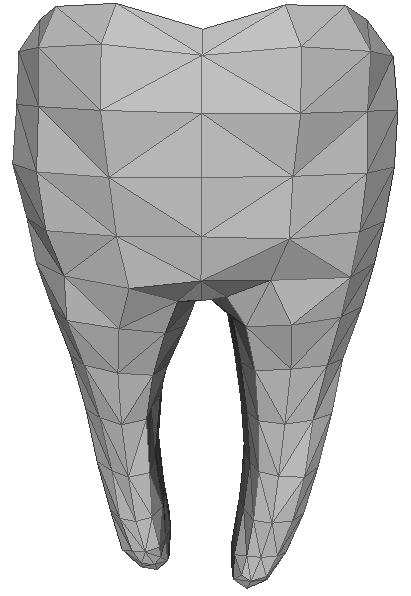
\includegraphics[width=0.32\textwidth]{./images/titlepage_highres.png}\\[0.5cm]


\textsc{\huge Aarhus University}\\[0.1cm]
\textsc{\Large Department of Computer Science}\\[0.1cm]
\textsc{\Large October 1, 2009}\\[1.0cm]


\textsc{\Large
%  Authors: \\
  Christian P. V. Christoffersen \\
  cpvc@cs.au.dk \\
  20050879  \\
\vspace{5mm}
  Carsten Nørby \\
  tic@cs.au.dk \\
  20051359
}\\[0.8cm]


\begin{minipage}{0.9\textwidth}
\HRule \\
\end{minipage}\\[0.0cm]

\textsc{\Large
\begin{tabular}{c c c}
  Primary Supervisor & & Secondary Supervisor \\
  Associate Professor & \hspace{5mm} & Associate Professor \\
  Ole Østerby & \hspace{5mm} & Thomas Sangild Sørensen
\end{tabular}\\[1.5cm]
}


% årskort 
% • name 
% • title 
% • supervisor’s name 
% • month and year 
% • the phrase “Master’s Thesis” 





% \textsc{
% \begin{tabular}{c c c}
%   Author & & Author \\
%   Christian P. V. Christoffersen & \hspace{10mm} &Carsten Nørby \\
%   cpvc@cs.au.dk & \hspace{10mm} & tic@cs.au.dk \\
%   20050879 & & 20051359
% \end{tabular}\\[1.5cm]
% }

% \title{
%   Real-time Fragmentation of Solid Material \\
%   using the Finite Element Method
% }

% \date{\today}

 
 
% \textsc{\LARGE University of Beer}\\[1.5cm]
 
% \textsc{\Large Final year project}\\[0.5cm]
 
 
% % Title
% \HRule \\[0.4cm]
% { \huge \bfseries Lager brewing techniques}\\[0.4cm]
 
% \HRule \\[1.5cm]
 
% % Author and supervisor
% \begin{minipage}{0.4\textwidth}
% \begin{flushleft} \large
% \emph{Author:}\\
% John \textsc{Smith}
% \end{flushleft}
% \end{minipage}
% \begin{minipage}{0.4\textwidth}
% \begin{flushright} \large
% \emph{Supervisor:} \\
% Dr. Mark \textsc{Brown}
% \end{flushright}
% \end{minipage}
 
% \vfill
 
% % Bottom of the page
% {\large \today}
 

\end{center}
\end{titlingpage}
%\end{titlepage}
%\end{document}

\cleardoublepage

% title page
%\maketitle
\thispagestyle{empty}


%\input{cover_page}
\cleardoublepage % to insure that the page numbering is correct

\pagenumbering{Roman}
\pagestyle{plain}

%\pagestyle{empty}
% -*- mode: latex; mode: auto-fill; coding: utf-8; -*-

\begin{center}
\begin{minipage}{0.7\textwidth}
\chapter*{Summary}
% What?
This thesis is within the field of simulated surgery and motivated by
the current demand for an educational tool 
teaching the common procedure of wisdom tooth extraction.
Attention is focused on how to simulate the fragmentation 
that will separate the crown of the tooth from its roots.
%
% How
We present a general method for crack prediction and propagation in
volumetric solids based upon
real-time structural analysis. The analysis is conducted using the
finite element method and the Total Lagrangian Explicit Dynamics
solving technique with a parallel approach.
%
The stress and strain analysis are based on 
the theoretical laws of physics and the crack prediction is based on
the theory of maximum principal stress from fracture
mechanics.
%
% So?
%
The failure surface as predicted by the
crack tracking algorithm looks very promising. The location and
curvature of the failure surface corresponds to the stress analysis
and the intuition of how an object would actually fracture.
%
Benchmarking the simulation model reveals great potential towards
real-time interaction and visual feedback.
\end{minipage}
\end{center}
%\thispagestyle{empty}
% -*- mode: latex; mode: auto-fill; coding: utf-8; -*-

\chapter*{Acknowledgement}
We greatly appreciate all who contributed to this thesis,
especially the following people who we would like to give a special
thanks to: \\ 

Associate Professor, Ole Østerby for supervision, guidance, and
for always leaving his door open, both literary and figuratively. We
are grateful for all the time he spent carefully explaining theories
to us and for his comprehensive reviews. 
%
Associate Professor Thomas Sangild Sørensen for supervision, especially within the field
of simulated surgeries and for all the inspiring talks, ideas,
references, reviews, and guidance throughout this entire thesis.

%
PhD student, Karsten Østergaard Noe, for sharing his knowledge and
a prototype solver for structural analysis. \\

PhD Jesper Mosegaard and Peter Trier, from The Alexandera
Institute, for introducing the problem domain, their cooperation and
for establishing collaboration with people from the Aarhus School of
Dentistry, Aarhus University. \\

Professor, dr.~odont.~Søren Schou, Aarhus School of Dentistry, Aarhus
University, for his enthusiasm and all the time he spent on carefully
explaining how dental surgical procedures are performed. We are
thankful for all the material he provided including books, videos,
dental instruments, wisdom teeth and for granting us the permission to
use the dental pictures included in this thesis (marked by \textdagger). \\

PhD student, Lau Brix, for guidance concerning hardware
configuration for a high performance computer suitable for parallel
execution
%
and the Siemens foundation (Siemensfonden) for funding this
hardware.
%
Christian Esbo Agergaard, 3D artist, for creating a three-dimensional
surface mesh of a wisdom tooth, which is suitable for our simulation
scenarios.
%
The OpenEngine community for providing the portable framework used as
the foundation for the simulator implementation.

\cleardoublepage
\thispagestyle{empty}
% -*- mode: latex; mode: auto-fill; coding: utf-8; -*-

\chapter*{Reader's Guide}
This thesis consists of three parts. Part I presents analytical
theories. This part includes statics, dynamics, continuum, and fracture
mechanics. Futhermore, elasticity theory and basic linear algebra is
introduced. Part II presents discrete theories. Here the fundamental
equilibrium framework and the finite element method are explained in
detail and used to construct a simulation model. Part III explains how
the simulation software is designed and implemented. Parallel
execution is introduced and the simulation software constructed is
evaluated.
%
The following is a brief summary of each chapter: \\ 

Chapter \ref{chapter:introduction} introduces the reader to the field
of simulated surgery and the potential of computer aided simulations
in general. Here the motivation behind this thesis is stated.
%
Chapter \ref{chapter:problem_domain} explains the surgical procedure
of wisdom tooth removal step by step. The physical phenomena of
interest are identified and the concepts real-time and simulator are
defined. The main objectives in the thesis are stated and related work
are presented.

\section*{Part I - Analytic Theories}
Chapter \ref{chapter:physics} introduces the fundamental physics
used. Work, energy, and equilibrium are defined before moving on to
continuum mechanics where the concepts deformation, elasticity,
stress and strain are introduced.
%
Chapter \ref{chapter:mathematics} explains the basic linear algebra
used.

\section*{Part II - Discrete Theories}
Chapter \ref{chapter:equilibrium_framwork} introduces the fundamental
structure for equilibrium problems in general.
%
Chapter \ref{chapter:finite_element_method} describes the finite
element method. The discretization of the continuum body and how
to assemble the system equations are explained in detail.
%
Chapter \ref{chapter:applying_finite_element_method} explains how to
apply the finite element method and a concrete solver technique is
presented.

\section*{Part III - Implementation}
Chapter \ref{chapter:simulation_model} presents the simulation
software developed.
%
Chapter \ref{chapter:parallel_execution} introduces the concept of
parallel execution and explains how we utilize NVIDIA's CUDA
technology.
%
Chapter \ref{chapter:helper_tools} explains the developed tools for
interacting with the simulation software and how to visualise
tensors.
%
Chapter \ref{chapter:results} presents the results obtained.
%
Chapter \ref{chapter:future_work} is a discussion on possible
improvements.
%
Chapter \ref{chapter:conclusion} summarizes and concludes on the
results obtained. 

\cleardoublepage

\pagebreak % to insure that the page numbering is correct

\cleardoublepage
%\pagenumbering{roman}
%\pagenumbering{Roman}
\tableofcontents*
\cleardoublepage
\listoffigures*
Figures marked by the following symbols are from external sources:
\begin{center}
\begin{minipage}{0.9\linewidth}
\begin{tabular}{c l}
\textdagger & Image provided by Søren Schou, Aarhus School of
Dentistry. \\[3pt]
$\ddagger$ & From NVIDIA's CUDA Programming Guide (Version 2.3.1).
\end{tabular}
\end{minipage}
\end{center}
\cleardoublepage
\listoftables*
\cleardoublepage
%\include{symbols}
\pagebreak

\pagenumbering{arabic}
%\pagestyle{fancy}
\pagestyle{mystyle}

% Code for creating empty pages
% Use plain style on empty pages before new chapter
% \makeatletter
% \def\cleardoublepage{\clearpage\if@twoside \ifodd\c@page\else
%   \hbox{}
%   \thispagestyle{empty}
%   \newpage
%   \if@twocolumn\hbox{}\newpage\fi\fi\fi}
% \makeatother \clearpage{\pagestyle{empty}\cleardoublepage}

\chapter{Introduction}
\label{chapter:introduction}
% -*- mode: latex; mode: auto-fill; coding: utf-8; -*-

%\chapter{Introduction}
% - simulator
% - real time
% - soft tissue + hård materiale
% Set the scene, fixed object, apply forces, eventually break the
% object into smaller pieces.

The research field of computer simulated surgery has been a
topic of increased interest in recent years.
%
The current research has reached a level that facilitates
real-time simulation of deformations in soft organic materials. 
%in high-resolution on consumer hardware. 
Using computer aided simulations as an educational
tool or an interactive training facility has a lot of potential when
it comes to imparting new knowledge to students or
trainees. Surgical procedures can be studied and practiced iteratively
through extended feedback including any imaginable visual
information. While performing the simulated surgery instructions and
guidance could be presented, any potential risk could be pointed out,
and unexpected critical scenarios could occur. 
Simulated surgery has the potential to enrich the
learning process on so many levels.  
%
From the perspective of
the student the main objective of using simulated surgery is to
acquire certain, often very difficult, skills in a risk-free
environment. Introducing surgical certificates based
on simulations is an option within the near future. Professional approval
based on simulated scenarios has been used for many years when
educating and certifying pilots. \\

% Challenges and limitations 
The field of simulated surgery still faces great
challenges especially when it comes to the sense of touch. It is
very difficult to simulate the correct feedback on the tool being
used e.g. the weight, friction, momentum, manoeuvrability
etc. Simulation models based on the laws of physics will
always be idealized and respond as predicted by theory. Sometimes
theory and practice is not consistent. \\
%
% With attention focused on improving the visual feedback there
% is a lot to benefit from simulated surgeries. 

%
The development within computer aided visualization has been
tremendous during the last decades. The research within this field
has benefited heavily from the huge investments made by the
entertainment industry constantly striving towards improving the level
of realism. 
%
Simulating organic material like human tissue or organs require a
model capable of representing the complex structures and
the theoretical laws of behaviour. 
%
In the field of applied mathematics a generalized method for
conducting numerical modeling of physical systems was first well
defined in the late 1960's and early 1970's. 
%
Although these mathematical models are capable of capturing
complicated problems they tend to get very complex and computationally
expensive.
%
Within recent years the introduction of multi-core hardware and the
development in GPU programming languages, suddenly has made these
models, based on the actual laws of physics, realisable. By taking
advantage of the parallel architecture of the GPU, the computational
resources have increased by orders of magnitude assuming the problem
can be solved in a parallel environment. \\

%In recent years the research field within computer simulated surgeries
%has increased drastically. 
%
% The increasing interest for simulated surgeries used as an educational
% tool or interactive training facility is probably due to the
% fact that the current level of research now facilitates
% real-time simulation of organic materials in high-resolution.
% %
% The mathematical models capable of representing problems within the
% problem domain of simulating complex structures have been developed
% in modern times. In applied mathematics a generalized method for
% conducting numerical modeling of physical systems was first well
% defined in the late 1960's and early 1970's. 
% %
% The development within computer aided visualizations has been
% tremendous during the last decades. The research within this field
% have benefited heavily from the huge investments made from the
% entertainment industry constantly trying to improve the level of
% realism. 
% %
% Simulating organic material like human tissue and organs requires huge
% computational efforts, but with the introduction of multi-core
% hardware and the development in GPU programming languages, models
% based on the laws of physics suddenly becomes realisable. \\
%

% Modern consumer hardware has gradually increased in
% computational resources to a level now facilitating real-time
% execution of interactive 
%

% Modern consumer hardware has gradually reached a level that now 
% facilitates real-time execution of plausible simulations based on
% mathematical models incorporating the laws of physics

% Background history
This thesis is motivated by the current demand for an educational tool
teaching a specific dental procedure. Inspired by related
simulated surgeries The Aarhus School of Dentistry has requested a
simulator for teaching the common procedure of wisdom tooth
extraction. Performing the surgical procedure requires certain skills
and must be
performed with caution to prevent serious nerve damage. All
surgery involves risks, in this case the patient's tongue or part of
the lip could become permanently numb due to nerve damage. This
emphasizes the importance of a proficiency before
operating on patients. Besides lots of lessons and videos teaching how
to perform the operation, students practise on a rubber doll known
as a \defit{phantom}. Operating on a phantom is the last step before the
students are expected to perform supervised operations on
patients. According to Professor, dr. odont. Søren Schou, Aarhus
University, there is a huge educational gap between operating on a
phantom and a real patient. \\

%This thesis deals with the design and implementation of a model
%This thesis deals with the development of a simulation model based on
%structural analysis using the laws of physics to simulate 
This thesis deals with the development of a model for simulating one
specific part of the complete surgical procedure of wisdom tooth
removal.
%
Attention is focused on how to simulate the fragmentation
that will separate the crown of the tooth from its roots. 
By solving this particular problem we get one step closer
towards the development of a complete simulator, handling the entire surgical
procedure, hereby providing an educational tool
with the purpose of minimizing the gap between operating on a phantom
and a real patient. \\

The simulation model
is based on the finite element method which is a widely accepted
method for structural analysis. The physical laws from the field of
continuum and fracture mechanics concerning deformation and
fragmentation of solids are applied to obtain as realistic
results as possible with the computational resources available. \\

% Explain to humans what the simulator is - MVC pattern
Basically the simulator consists of three main parts. A visual,
an interactive, and a computational part. The visual part is
responsible for delivering real-time three-dimensional images on the
screen. The interactive part handles the user interaction and
simulates the dental tools accordingly. The computational part 
is responsible for solving the equations defined by the method used
for the structural analysis. \\

% Interdisciplinary approach
It requires an interdisciplinary approach to develop a framework for
simulating deformations and possible fractures in solid objects. 
From the field of dentistry, knowledge on how to perform the actual surgical
procedure, is needed. 
%
Simulating real world phenomena of
fracturing solid objects involves theoretical physics and mathematics, as well as
engineering disciplines of predicting how solids behave under
stress. 
%
Constructing a computational model representing the complex structures
that incorporates the laws of physics suitable for high performance
parallel execution is a computer science discipline. Implementing the
simulator using the proper technologies, benchmarking the
software model and validating the results are all within the
field of computer science. 

% The main emphasis here is on how to
% assemble the relevant theory in the construction of a valid model what
% will be real-time executable



\doubleblank

\chapter{Problem Domain}
\label{chapter:problem_domain}
% -*- mode: latex; mode: auto-fill; coding: utf-8; -*-

\section{The Surgical Procedure}
\label{sec:surgical_procedure}
% The learning process
To gain fundamental knowledge on how the surgical procedure is
performed in real life, the following section will explain each step
involved. This section is based on an interview with Professor,
dr. odont. Søren Schou, Aarhus University, who carefully took his time
to explain the procedure in detail.  \\

% Explain briefly the four scenarios
First of all when it comes to patients with wisdom tooth compilations,
there are not two of a kind, but basically all complications can be
divided into four scenarios. Within each scenario the location of the
tooth can vary but the approach used to remove it is the same. The
four scenarios are illustrated in figure
\vref{fig:wisdom_tooth_scenarios}. The different scenarios require
slightly different approaches when it comes to fragmenting the
tooth. The following steps are carried out in each of the four
scenarios. \\


% \begin{figure}
%   \centering
%   \includegraphics[width=6cm]{./images/problem_domain_surgery_four_tooth_positions.png}
% \caption{The four basic scenarios showing how the wisdom tooth can be
%   located in the jaw.}
% \label{fig:wisdom_tooth_scenarios}
% \end{figure}

\begin{figure}[h]
    \centering
    \subfloat[Angular]{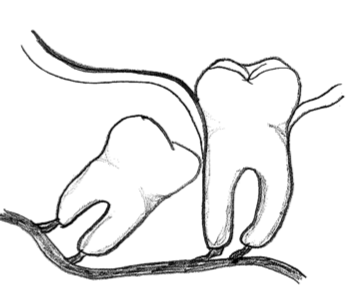
\includegraphics[width=50mm]{./images/problem_domain_surgery_tooth_0.png}}
  \hspace{0.5cm}
    \centering
    \subfloat[Partial Eruption]{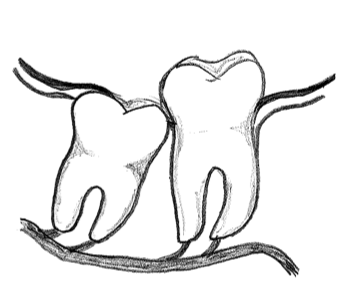
\includegraphics[width=50mm]{./images/problem_domain_surgery_tooth_1.png}}
  \newline
    \centering
    \subfloat[Horizontal]{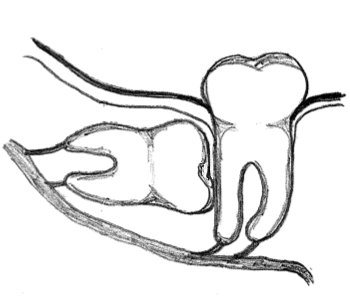
\includegraphics[width=50mm]{./images/problem_domain_surgery_tooth_2.png}}
  \hspace{0.5cm}
    \centering
    \subfloat[Vertical]{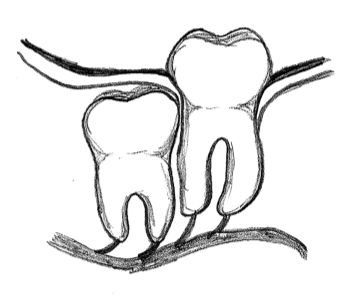
\includegraphics[width=50mm]{./images/problem_domain_surgery_tooth_3.png}}
\caption{The four basic scenarios showing how the wisdom tooth can be
  located in the jaw.}
\label{fig:wisdom_tooth_scenarios}
\end{figure}


As a preoperative task
the dentist carefully examines x-ray images of the wisdom tooth to determine
the risk of nerve damage. It is crucial that the nerves are left
undamaged since this can lead to complete and permanent numbness of
the tongue and lip.


\subsection*{Anaesthesia}
% local anaesthesia to the nerves in the jaw
The surgical procedure can be performed under local anaesthesia,
leaving the patient conscious during the entire operation. The local
anaesthesia is carefully injected directly into the nerves located on
the inside of the jaw,
making the tongue, part of the lip and the wisdom tooth numb. The
anaesthesia substance contains adrenaline which contracts the blood
from the blood vessels, hereby minimizing the bleeding from the wound.
% pinch to check anaesthesia 
Shortly after the anaesthetic injection, the dentist
pinches the surrounding tissue to ensure the area is numb. 


\subsection*{Incision}
% using scalp to perform the tissue cut
The soft tissue surrounding the wisdom tooth, on the outside of the
jaw, needs to be loosened to expose the tooth. 
% always on the outside of the jawbone
The cut starts from the back of the jaw and is carefully placed along the
outside of the first and second molar, illustrated as the red line in
figure \vref{fig:incision_cut}. The yellow dot is where the wisdom
tooth is located, currently covered by soft tissue. It is crucial not
to damage the nerve located on the inside of the jaw, therefore
the incision is always performed on the outside of the
molars.    
% Suction
The cut is made slowly while any blood from the wound is sucked away
with a small tube to keep visibility high and to prevent it from
running down the patients throat. 
%
When the incision has been made, the soft tissue can be pulled to the side hereby
revealing the wisdom tooth and part of the roots of the first and
second molar. 
% the wisdom tooth located down the jaw. 
Often the wisdom tooth is located deep down the jawbone so only the crown
of the tooth is visible when the soft tissue has been removed.

\begin{figure}
  \centering
  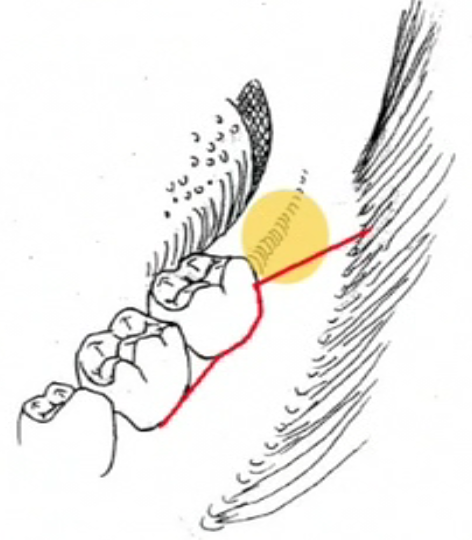
\includegraphics[width=4cm]{./images/problem_domain_surgery_incision.png}
\caption{The red line illustrates where to place the incision. \textdagger}
\label{fig:incision_cut}
\end{figure}

\subsection*{Bone Removal}
Now that the soft tissue is removed the next step is to remove the
surrounding jawbone. This is done using a drill on the outside of the
jaw as illustrated with the red line on figure
\vref{fig:bone_removal}. Drilling away the surrounding jawbone will
expose the wisdom tooth down below its crown. When drilling, the point
of contact between drill and jawbone, is constantly cooled with 
water to prevent the nearby soft tissue from heating up potentially
causing damage.

\begin{figure}
  \centering
  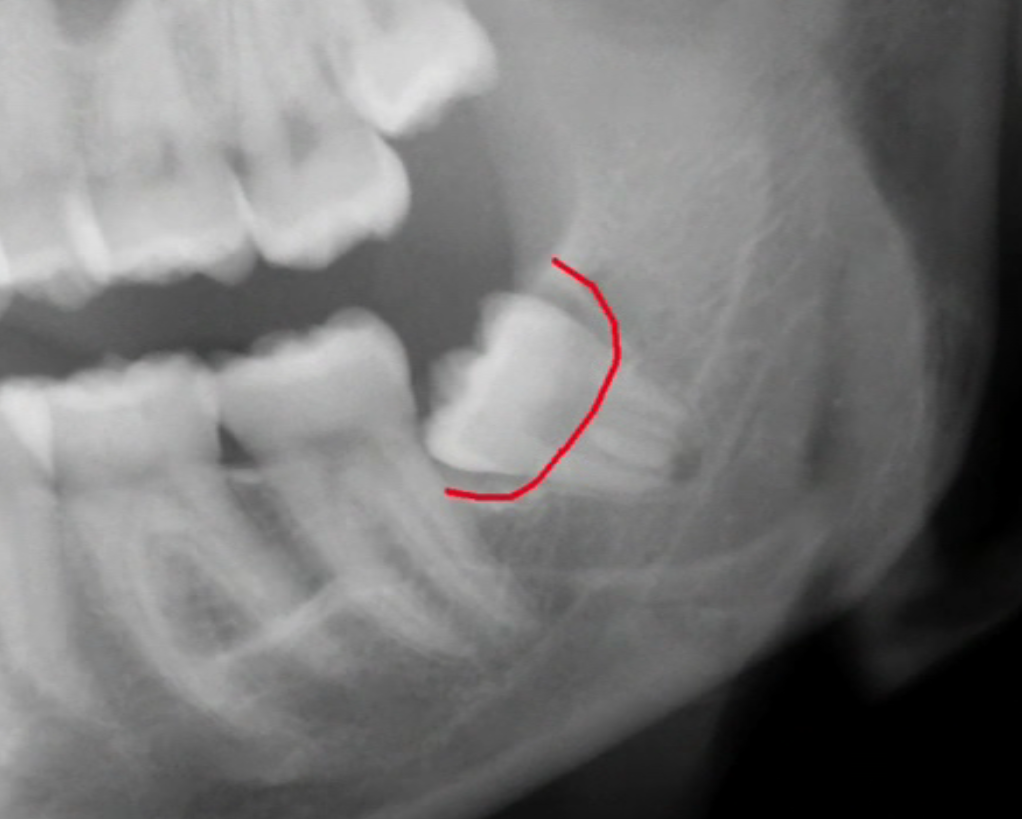
\includegraphics[width=6cm]{./images/problem_domain_surgery_bone_removal_xray.png}
\caption{The red line illustrates where the jawbone must be drilled
  away. \textdagger}
\label{fig:bone_removal}
\end{figure}

\subsection*{Drilling a Groove}
Now that the wisdom tooth has been exposed from both the surrounding
tissue and jawbone, the dentist can move on and prepare a controlled
fragmentation of the tooth. The fragmentation must carefully separate
the crown of the tooth from its roots as illustrated by the red line
in figure \vref{fig:groove_line}.
A straight groove is drilled along the red line, as illustrated on figure
\vref{fig:groove_line}. The groove is approximately
5 millimeters deep, or one third of the tooth, and located right below
the crown. 

\begin{figure}
  \centering
  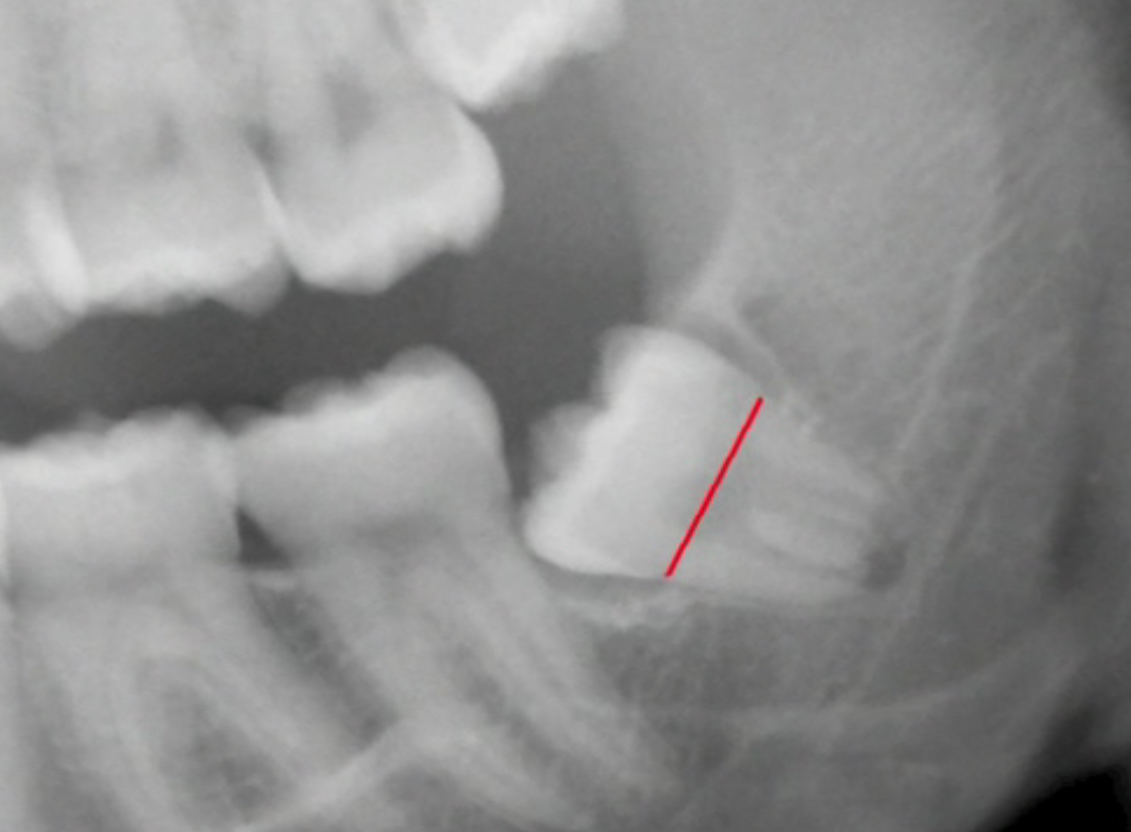
\includegraphics[width=6cm]{./images/problem_domain_surgery_fragmentation_line.png}
\caption{The red line illustrates where the groove should be drilled. \textdagger}
\label{fig:groove_line}
\end{figure}

The dentist always tries to avoid drilling down the enamel on the
crown of the tooth, because it is so hard that the drill will be worn
down too fast.  

\subsection*{Fragmentation}
A special tool known as an \defit{elevator}, illustrated in figure \vref{fig:elevator},
is now inserted into the groove and twisted to separate the crown of
the tooth from its roots. Sometimes, due to the location of the wisdom
tooth, it is necessary to perform further fragmentation to either the
crown or the roots. 

\begin{figure}
  \centering
  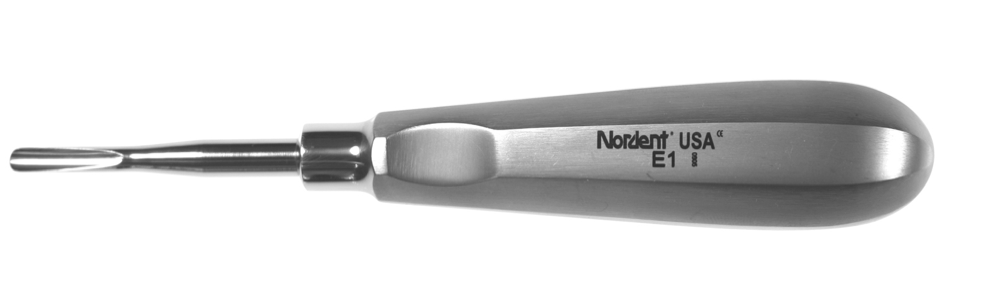
\includegraphics[width=8cm]{./images/problem_domain_surgery_elevator.png}
\caption{Dental tool known as an elevator. \textdagger}
\label{fig:elevator}
\end{figure}


\subsection*{Fracture Removal}
Now that the tooth has been fragmented the individual parts must be removed carefully.
It is very important to make sure all of the fragments are
removed properly. If a small piece is left behind it can cause
complications such as wound infections. 
%
Usually wisdom teeth are removed only if they cause some sort of
complications. A common complication is when other teeth prevent the natural
development, often causing an small infection around the wisdom
tooth. The infected tissue must be removed from the wound as well.      

\subsection*{Smooth Off the Rough Edges}
The dentist has to smooth off the rough edges in the jawbone to
prevent complications with the soft tissue surrounding it.
The crater from where the wisdom tooth was located, must be cleaned
thoroughly with water to wash out every tiny bit of bone from the
drilling. 

\subsection*{Stitching the Wound}
The last step in the surgical procedure is to stitch the wound together. Usually two
stitches is enough but this depends on the size of the
wound. When the stitching is done a small cloth is inserted in the
cheek to absorb any remaining blood. The surgical procedure is now
done.

\section{Simulator}
\label{sec:simulator}
% What is a simulator? (real-time, high-performance workstation)
In context of computer science a simulation is a computational model
that approximates a real phenomenon or procedure. A simulation defines
rules of behaviour reflecting those appearing in the real world. The
results produced by a simulator can be used for evaluation or
prediction of the phenomenon or procedure simulated.  
%
Challenges arise due to the almost unlimited complexity of any real world
phenomena no matter how simple it seems.
Specific parts of the phenomenon being
simulated must be prioritised, but even then only a certain level of detail
can be computed. 
%
If time and computational resources was no issue, designing a
model that strictly represents solid objects by the smallest unit
possible, would be a solution. 
However intuition tells us that it is probably impossible to represent and 
simulate the physical laws for such small units. Let us consider atoms
as the basic unit of matter, the nucleus diameter of an atom is about $10^{-15}$
meter. Even for a small object like a tooth the amount of units to
be represented would be billions, easily exceeding the computer
resources available. A discrete method must be used in order to
facilitate computation of the problem domain. 


\subsection{Real-time}
\label{sec:real-time}
It is crucial that the simulator gives the impression of a surgical
procedure performed in real-time. 
% Real-time
The concept of simulated real-time can be considered from two
different perspectives. One way is to measure real-time as the speed
of average sensory perception. By measuring real-time this way we consider 
how fast the system is responding to an event such as user
interaction. In this sense real-time is more of an illusion where
users should perceive the simulation feedback at a rate that 
corresponds to the actual scenario in real life. 

\begin{quote}
\defit{"
It doesn’t really matter whether the deformation that the surgeon sees
in the virtual environment is accurate as long as it seems realistic!
Just as important is that the model is robust and shows a consistent
and predictable behavior over time"}
\begin{flushright}
%\hspace{30mm} 
(Morten Bro-Nielsen
\citebook{page~8}{article:bro-nielsen})
\end{flushright}
\end{quote} 

%
Another way of defining real-time is to consider 
the extrapolate of simulation time contra the computation time
used. When simulating a phenomenon time must be discretized into time
steps that represents the difference in time from the current
configuration to the next. If it is possible to compute the next
configuration faster than the time extrapolation it represents we can
predict the behaviour of the phenomenon in real-time. If not we can
pre-compute the behaviour and inspect them at a real-time rate
afterwards, but this rules out real-time interaction which is an
essential part a surgical simulator. \\

To accommodate the demand for real-time execution appropriate solving
techniques must be used. A variety of limitations and approximations
must be taken into account to keep the result plausible. 
When the level of simulation details increases so does the
computational efforts. Making the right decisions in the trade-off
between accuracy and speed is essential. 
%
Each time an
approximation is made the margin of error must be considered to
prevent the final result from ending wide of the mark. 


% Simulation time progresses by the rate of a pre-computed
% time step. The size of the time step is base upon the approximate
% speed of sound waves traveling through the given material. Using this
% definition the simulated time step is representing actual time.  
% %
% If it is possible to compute the simulated time step faster than
% the actual time it represents the simulation is executable in
% real-time.
%

% %
% % As we shall see later some methods used when predicting the next
% % configuration introduces limitations on how fast time exploration can
% % be done.
% %
% When the level of simulation details increases so does the
% computational efforts. Making the right decisions in the trade-off
% between accuracy and speed is essential. 
% %
% Each time an
% approximation is made the margin of error must be considered to
% prevent the final result from ending wide of the mark. 


\subsection{Phenomena}
Before designing a model that represents the processes
we would like to simulate, we need to identify the physical
phenomena. 
% Types of material and their properties. (zoom to see atom grid)
It is no surprise that different materials behave very
differently. Dropping a glass vase on the floor would probably break
it while a rubber ball would bounce back without a scratch. What might
be a surprise to some, is the rather complex physical theory behind
this. The answer to why some materials are able to undergo change in form without
breaking and others are not, lies in the structure of the
molecules. Since representing a material on the level of molecules
would exceed the computational resources, this phenomenon must somehow be
represented on a higher level.  \\

% Energy and elasticity
A rubber ball can deform into an ellipsoid and still return to its
original form. In physics elasticity is the property that
makes a material deform due to external forces, but still makes it
return to its original form when the external forces are removed. This
phenomenon requires a model where external forces somehow are transformed into
elastic energy. \\


% Forces applied to a material causes deformation and induces internal stress, 
% the relative amount of the deformation is referred to as strain. 
% There exists a variety of ways
% to represent elasticity but basically it represents the relation
% between stress and strain. Elasticity, stress and strain are
% fundamental physical concepts that must be understood and incorporate
% into the simulation model. \\   

% Homogen vs. non-homogen
A homogeneous material contains only identical molecular structures
and is therefore a pure material with the exact same properties
everywhere. In the real world this is rarely the case, most materials are a
composition of others. A tooth has different layers each
with different material properties. From that perspective modelling
heterogeneous materials would probably be preferable. \\

% Temperature impact on diff. materials 
It is common knowledge that most material properties change as a
result of change in temperature. When steel is heated its strength
decreases, and rubber cooled down to extremely low degrees can shatter
like glass. Decision must be made whether or not to represent this
phenomenon in the simulation model. \\  

% Fragmentation 
When things break in the real world it often happens in a blink of an
eye. A rule of thumb says that a crack propagates through a brittle
material with the speed of sound. Observing the propagation would
require a 
high speed recording of the phenomenon for later replay in slow motion.
Intuition tells us that the crack must have a point of origin. As the
crack propagates through the material it must somehow choose its path
based on the material properties and the external forces acting upon
the material. 



\section{Problem Statement}
\label{sec:problem_statement}

% Define what part of the simulator we will focus on
As already mentioned the surgical procedure of removing a wisdom tooth
involves various steps of cutting tissue, drilling, fracturing dental
material, stitching tissue, etc. Simulating each step requires a
different approach and the use of distinct theory. It is out of scope
of a single masters thesis to handle all of the different step. \\

% would require a tremendous amount of work impracticable
% due to resources available.
%
Considering the relatively limited amount of work published
within the field of fracturing volumetric models in real-time
compared to the other fields of interest from the various simulation
steps, attention will be focused on solving this particular problem. \\

This thesis deals with simulating the specific parts of the
dental procedure that involves fragmentation of the tooth. Separating the
crown of the tooth from its roots involves estimation of the internal
stress and prediction of crack propagation through a solid material. 
%
The estimation of internal stress will be based on the finite element
method which is a widely accepted method used for structural
analysis. Using the finite element method to conduct real-time
analysis is a fairly new concept developed within recent years. It
has proved to be one of the most precise methods available.
%
The method for predicting the point of origin and the propagation of
the crack will be based upon the theory of maximum principal
stress. 
%
To the best of our knowledge the parallel approach of conducting real-time
structural analysis in conjunction with crack propagation, based
upon maximum principal stress is new to the field. \\

% Motivate deformation and fracture framework
The main objective in this thesis is to create a framework for
real-time simulations of deformation and crack initialization in solid
objects. 
%
With point of reference in the laws of physics we will
construct a simulation model that strictly complies with relevant
theory. The context of use is simulated surgery therefore speed
and robustness of the model will be favoured over accuracy.
%
External forces will be applied through a simulated dental tool, similar
to the elevator actually used by dentists. 
%
The stress and strain analysis will be based on 
the theoretical laws of physics and the crack prediction will be base on
the theory of maximum principal stress direction from fracture mechanics. 
%
We will construct a model aimed towards real-time crack detection
based upon analysis of stress and strain behaviour. If the
internal level of stress exceeds a material-specific threshold the
solid object will fracture. Once the point of origin of the crack has
been predicted the determination of the crack surface is not
considered time critical.


% Focusing on how to simulate the
% physical phenomena involved when applying external forces to a solid
% object and how to 


% A criterion of success is not to develop
% a simulation model which strictly complies with the theoretical laws of
% physics, but to achieve plausible results base on relevant theory. Speed
% and stability will be favoured over accuracy due to the demand of
% real-time execution. 

% The main purpose is to provide a
% realistic training facility and not to provide a framework for
% structural engineers. \\


\section{Related Work}
% Related work from Aarhus University
The purpose of solving the particular problem of how to
fracture solid material in real-time, is to establish a theory 
that will bring the development of a complete dental surgical
simulator one step closer to reality. The simulation model presented
in this thesis is base upon the combination of numerous theories and
existing methods. 
%
The following articles presents closely related work and methods
we have derived our simulation model from. \\

% First on real-time deformation using FEM
Morten Bro-Nielsen was among the pioneers
within real-time simulation of deformable models used for simulated
surgery. Morten Bro-Nielsen
\citeabook{article:fast_fem}\citeabook{article:bro-nielsen} presents a 
method base on a Fast Finite Element (FFE) method and linear
elasticity. The interior nodes
are removed from the equations to improve performance. Even though the
interior nodes are excluded from the calculations the predicted
behaviour of the surface nodes are exactly the same a if interior node
was taking into account. \\

% Miller
% Related work within the field of deformable models aimed towards use
% in surgery simulations, has been presented by
Miller et al. \citeabook{article:miller} present an efficient numerical
method for computing soft tissue in real-time, based upon finite
element analysis. Their method is based on total Lagrangian
formulation relating stress and strain to the original configuration. \\

% TLED
Zeike A. Taylor et al. \citeabook{article:tled} present an improved method
based directly upon the work conducted by \citeabook{article:miller}.
The improvements made are primarily on how to solve the finite element
equations in parallel using the GPU hereby gaining a significant
increase in performance. \\

% Real-time
Thomas Sangild Sørensen and Jesper Mosegaard presents methods on
how surgical simulations can accelerate deformable models through
the parallel nature of the GPU\citeabook{article:gpu_surgery}. They show
that deformable models based on the spring-mass or finite element
method can be implemented using parallel programming hereby gaining a
significant increase in performance. \\


% Fracture
Depending on how much the wisdom tooth is developed, fragmentation of
the tooth can be necessary. Teeth are primarily made of a material
called dentin which consists of calcium, phosphorus, and other
mineral salts. Dentin is a very hard and brittle material.
Techniques for simulating fracture initialization and
propagation in brittle materials has been presented by O'Brian
et al. \citeabook{article:brittle_fracture}. The method presented is based on
finite element analysis and aimed towards pre-rendered simulations. \\

% First real-time deformation and fracture of stiff materials
Matthias Müller et al. \citeabook{article:muller} present a method for
real-time deformation and fractures in stiff materials. The method
presented introduces a hybrid approach where the simulation is
alternating between simulating rigid body dynamics and the
continuum model at the point of impact. The fragmentation method used
includes model re-meshing which improves the realism of the crack
surface. \\ 

% Different fracturing methods
A comparison of different fracturing techniques has
been conducted by P. Jäger et al. \citeabook{article:crack_tracking_comparison}. The article
compares four different approaches in terms of standard quality
measures such as efficiency, robustness, stability and computational
cost.\\ 

Besides the closely related work, we have also paid attention to the
following articles and PhD theses presenting methods that could be
used for simulating the other parts of the complete simulator. \\

% Haptic feedback by Thomas Sangild
In relation to handling input the user, here being a surgeon,
must be presented to a device capable of simulating the tools similar
to the ones used in real life. Surgeons are used to manoeuvre tools
freely in three-dimensional space. An ordinary computer 
mouse has only two degrees of freedom which makes it unfit. Instead of
conventional user input like those of a keyboard or mouse,
we would prefer \defit{haptic} feedback. Haptic refers to the sense of
touch. In the context of surgical simulations it means a device that
interfaces with the user through force feedback. The haptic device
serves as a three-dimensional joystick with the extra feature of
delivering force feedback, when the virtual tool
intersects with an object in the simulator.
Handling user input immediately is crucial to prevent the surgeon from
experiencing latency and hereby loosing the illusion of real-time.   
Thomas Sangild Sørensen and Jesper
Mosegaard\citeabook{article:haptic_feedback} present efficient methods for
handling high-frequently haptic feedback using the GPU. \\

% Heart simulator
If the wisdom tooth is not developed enough the dentist will have to
cut the surrounding tissue to expose the wisdom tooth. As seen in figure
\vref{fig:wisdom_tooth_scenarios} the amount of tissue to cut open depends on the
location of the tooth.
Techniques for cutting soft tissue, based on a spring-mass model, has
been presented as part of a cardiac surgery simulator by Jesper
Mosegaard\citeabook{mosegaard2006Phd}. \\ 

% Ear simulator
When the wisdom tooth is exposed, the next step is to drill a hole into the
tooth as a preparation for the fragmentation.
A method for drilling in volumetric material in context of simulated
surgery has been developed by Peter Trier et al.
\citeabook{article:visible_ear}. The method is base on a data set 
available as a three-dimensional image format, and visualization
based on ray-castings. This technique has proved very promising. \\



\doubleblank

\part{Analytical Theories}
\chapter{Physics}
\label{chapter:physics}
% -*- mode: latex; mode: auto-fill; coding: utf-8; -*-

Physics is a science based on experiments where phenomena of nature
are observed with the objective of finding patterns and
principles. These patterns and principles are called theories or, when
they are commonly accepted, \defit{laws of physics}
\citebook{page~1}{book:uni-physics}.
%
As already touched upon in section \vref{sec:simulator}, the
simulator incorporates such physical laws to simulate
deformation and fragmentation of solid material. This
chapter introduces the physical theories needed to create a
 simulation model.
%
The aim is to assemble a theoretical model for deformation and
fragmentation based on the laws observed and generally accepted by
physicists.
%
Note that the physical laws used are idealized models, meaning
that the models are simplified versions of real phenomena and that
concepts of little importance for the overall result are neglected
\citebook{page~3}{book:uni-physics}.
%
In this respect we do not model material at the level of particles
as the effects of individual particles are not detectable when
larger volumes of matter are considered. This is called large-scale
mechanics in contrast to quantum mechanics, which deals with laws at
the level of atoms. Large-scale mechanics is valid when the size of
the material analysed is much larger than the size of an atom
\citebook{page~1}{book:continuum-mechanics}. \\

%A part of physics, \defit{mechanics}, are of special interest.
The subgroups of special interest are \defit{statics},
\defit{dynamics} and \defit{continuum mechanics}.
%
As the theory of continuum mechanics is quite complex, we will start
off gently by revisiting basic university physics in the context of
statics and dynamics. Here we define various physical quantities,
their corresponding units and how they are related.

% To get a visual image of the quantities, we need to set the
% scene \{tic}{we need to identify what needs to be modelled?}. 
% So what needs to be modeled? The basic idea is to manipulate an object
% through \defit{forces}. The object should react
% realistically and naturally to these forces. This object can be made of
% different material and have diverse shapes.\{tic}{The object
%   material and shape can vary.}

\section{Statics and Dynamics}
In statics, we only analyse objects that do not move. This enables
us to describe and relate various phenomena acting upon an object.
%
The next step is dynamics, where objects are allowed to move
but not to deform. Dynamics expands the analytical
method by allowing movement and rotation.
%
In statics an object is viewed as a single point which describes its
position. In dynamics objects are modeled by their position and
orientation. Statics and dynamics make these assumptions so objects
are less complex to analyse. In continuum mechanics objects are
represented by volumetric elements, which are more complex.

%define: space, time and reference frame
\subsection{Space and Time}
Within statics and dynamics, objects and forces alone are not enough
when analysing a physical system. The concept of an object at
rest or in motion requires a \defit{frame of reference}. A frame of
reference is any kind of coordinate system which enables us to uniquely
define the position of a body in three-dimensional space. To
describe motion the frame of reference must be fixed so only motion of
the moving body is considered.
%
By introducing time we can refer to an object at a given
time, hereby describing the object's \defit{velocity}
and \defit{acceleration}.
%
Complying with the SI system for units, distance is measured in meters
($m$), time in seconds ($s$), velocity in $m/s$, and acceleration in
$m/s^2$.

%interne vs externe forces, body and surface forces (static p. 78-80).
\subsection{Forces}
In mechanics there are many different types of forces,
therefore we need some basic terms to describe them. A force has a
direction and a magnitude. The direction is referred to as the
\defit{line of action}. The magnitude determines the size of the
force and is measured in newton ($N$). A force acts upon an object at
a specific point as illustrated in figure
\vref{fig:gravitationalforce}: A force is depicted in a
\defit{free-body diagram} as an arrow mounted at the point in which it
acts.

\begin{figure}
  \centering
  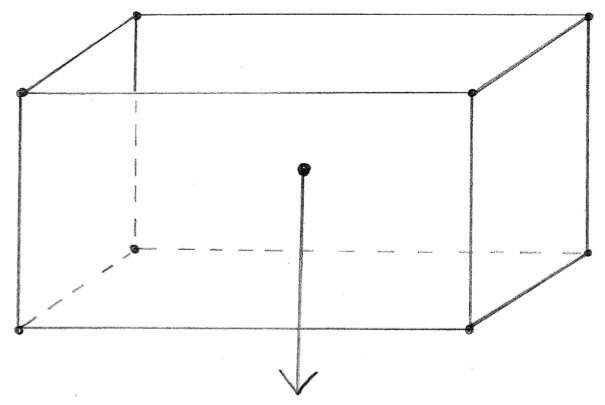
\includegraphics[width=6cm]{./images/physics_gravitationalforce.png}
\caption{Free-body diagram of the gravitational force acting upon a box.}
\label{fig:gravitationalforce}
\end{figure}

In mechanics an object is composed of two distinct concepts: a
\defit{surface} and a \defit{body} (note that the entire object is
often referred to as the body, which can be a little confusing).
%
Forces can be divided into different types, the types used in this
thesis are: body contra surface and internal contra external.
%
External forces act upon a physical system from the outside and can
not be generated by the system itself. 
%
An example of an external body force is the gravitational force as
illustrated in figure \vref{fig:gravitationalforce}. 
When two objects collide, a contact force occurs between
the colliding surfaces. This is an example of an external surface
force, and is illustrated in figure \vref{fig:contactforce}.
%
Internal forces do not occur in statics and dynamics because the
various internal parts of an object cannot move and hereby
interact. When modelling deformations, various parts of an object
can interact, hence we need internal forces.
In section \vref{sec:internal-forces} internal
forces will be introduced.

\layoutnewpage

% \begin{figure}
%   \centering
%   \includegraphics[width=6cm]{./images/physics_contactforce.png}
% \caption{A contact force.}
% \label{fig:contactforce}
% \end{figure}

\begin{figure}
  \centering
  \subfloat[]{
    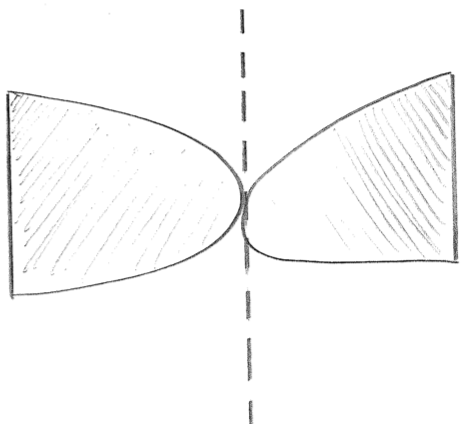
\includegraphics[width=6cm]{./images/physics_contactforce_a.png}
    %\label{fig:worka}
  }
  \subfloat[]{
    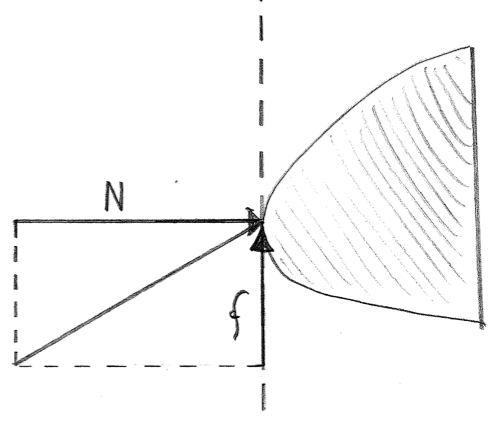
\includegraphics[width=6cm]{./images/physics_contactforce_b.png}
    %\label{fig:workb}
  }
  \caption{A contact force.}
  \label{fig:contactforce}
\end{figure}

Forces can be represented by vectors and therefore be resolved into
components. Resolving a force into its components sometimes eases the
analysis of a problem. Figure \vref{fig:contactforce} illustrates the contact force
resolved into two components $N$ and $f$, defined as the force normal
to the contact plane and a friction force along this plane,
respectively \citebook{page~80}{book:static-mechanics}.

\subsection{Equilibrium}
\label{sec:equilibrium}
To analyse a problem in physics, for example a free-body diagram,
the notion of equilibrium is used.
%
Equilibrium in general means an unchanging state or a state of
balance. In mechanics \defit{equilibrium} is defined as:

\begin{definition}
\label{def:equilibrium}
A body is in equilibrium if it is either at rest or moving in a
straight line with constant velocity \citebook{page~97}{book:uni-physics}.
\end{definition}

If a body is in equilibrium we can use definition
\vref{def:equilibrium} to analyse entities influencing the object's
behavior.
%
Depending on what types of problems we consider and which kind of
results we are seeking, this definition of equilibrium must be
interpreted differently to meet the constraints imposed on a given
problem.
%
We now consider three interpretations of the definition, with
increasing generality of the problems they capture, in each step
lowering the number of constraints imposed on the problem. \\

% equilibrium (static p. 205 and 273)
\subsubsection{Equilibrium for Fixed Objects}
\label{sec:equilibrium_for_fixed_objects}
When more than one external force act upon an object, the forces can
be added to yield the \defit{sum of forces}. The sum of forces is the
effective net force acting upon the body. We use this knowledge to
establish equilibrium for fixed objects.
%The sum of forces is calculated by: $\sum f = f_1 + f_2 + ... + f_n$.
Statics define equilibrium as \defit{conservation of forces} defined by:

\begin{definition}
\label{static-equilibrium}
A body that can be modeled as a particle is in equilibrium whenever
the vector sum of the forces acting on it is zero.
That is: $\sum f = 0$
\citebook{page~329}{book:uni-physics}.
\end{definition}

We can use this definition of equilibrium to analyse problems involving
fixed objects. That is: We can calculate unknown forces. Imagine that
we apply external gravitational force to an object placed on a
table. With the equilibrium equation we can calculate the force
provided by the table to support the object. \\

\subsubsection{Equilibrium for Moving Objects}
Equilibrium for fixed objects does not apply to moving bodies. In order
to model motion, more theory is needed. The simplest moving body is a rigid
body. A rigid body is allowed to move but not to deform. 
Movement has two distinct components: \defit{translation} and
\defit{rotation}. When applying the theory of equilibrium on rigid
bodies, translation and rotation must be included into the definition
of equilibrium.

\begin{definition}
\label{dynamic-equilibrium}
In addition to the requirements of equilibrium for fixed objects, the
sum of all torques due to all external forces acting on the body, with
respect to any specified point, must be zero.
That is: $\sum f = 0 \wedge \sum m = 0$
\citebook{page~329-330}{book:uni-physics}.
\end{definition}

\defit{Torque} or \defit{angular momentum} is a measure of a
rotational force. Torque is defined as: $m = r \times f$, where the force
$f$ is acting on a line of action perpendicular to the \defit{lever arm}, in
a distance of $r$ \citebook{page~294-296}{book:uni-physics}. Note that
equilibrium for fixed objects is a subset of equilibrium for moving
objects, and is exactly the special case where all torques are zero. \\

% \subsubsection{Equilibrium for Deformable Objects}
% Even with equilibrium for moving objects we do not capture the entire
% problem. As we want to model deformations we need to introduce
% continuum mechanics.
% In continuum mechanics we can no longer view the body as a single
% point, instead infinitesimal calculus is used for analysing the body.
% %
% To enable equilibrium analysis of a continuum we introduce the more
% general definition: \defit{mechanical equilibrium}. This definition is
% an alternative definition of equilibrium which can be apply to
% \defit{conservative} systems, and used in collaboration with
% infinitesimal calculus and continuum mechanics:
% %
% \begin{definition}
% \label{mechanical-equilibrium}
% An object is in mechanical equilibrium if the forces that do work as
% the result of a virtual displacement are conservative, i.e. the change in
% the total potential energy is zero: $\delta \Delta E_U = 0$
% \citebook{page~573}{book:static-mechanics}.

% %A system is in mechanical equilibrium if its position in configuration
% %space is a point at which the gradient of the potential energy is zero.
% %\citebook{page~?}{}
% %http://www.economicexpert.com/a/Mechanical:equilibrium.html
% %***gradient of the potential energy = forces, uni-physics, p. 215

% \end{definition}

% To understand this abstract definition, we introduce the terms:
% \defit{work}, \defit{energy} and means of \defit{conservation}. We
% also need to define what means \defit{virtual}, in context of
% mechanics. Again we note, although this time not directly apparent,
% that equilibrium for moving objects is a subset of mechanical
% equilibrium. The theory of continuum mechanics is further elaborated
% in section(\vref{sec:continuum}).


\subsubsection{Equilibrium for Deformable Objects}
\label{sec:equilibrium-for-deobj}
When considering deformable objects, we no longer use forces as
the quantity to define equilibrium.
%
% \{To explain why, we consider the following. 
% When a body is deformed by external forces the
% internals of the body are stretched or compressed generating internal
% forces. The external forces acting upon the body can in opposite
% directions. If the forces are of the same
% magnitude and in opposite directions then their sum  will be zero.
% Clearly this is not enough information for the body to bounce back,
% when the external forces are released. To record enough
%   information both the distance and direction in which the forces
%   stretch or compress the body must be taken into account.}
%
To define equilibrium for a deformable object, we will instead used
the \defit{principle of conservation of energy} as defined in
definition \vref{def:pmpe}.
 
\begin{definition}
\label{def:pmpe}
The mechanical energy in a conservative system is always constant
\citebook{page~160}{book:dynamic-mechanics}.
\end{definition}

In order to understand definition \vref{def:pmpe} we need to
introduce: work, kinetic energy, conservative systems, potential
energy, and mechanical energy. Again we note, although this time not
directly apparent, that equilibrium for moving objects is a subset of
equilibrium for deformable objects. In section \vref{sec:continuum},
when the theory of continuum mechanics is elaborated, we will return
to what equilibrium is for a deformable object, in that section it will be
applied to a continuum.

\subsection{Work}
\label{sec:work}
% enhed N*m = J, uniphysics p. 165
\defit{Work} is the amount of energy transferred by a force acting over a
distance. For a moving body where forces are not uniformly distributed
work is defined in terms of \defit{differential work}. So to calculate
the total work $W$ we
integrate $dW$, where $dW$ is the differential work done by $f$ as a
result of the displacement $dr$. Work is measured in Newton meter
($Nm$) or Joule ($J$) \citebook{page~174-179}{book:uni-physics}.

\begin{equation}
  dW = f \cdot dr = (|f|cos \phi)|dr|
  \qquad \Leftrightarrow \qquad
  W = \int dW = \int f \cdot dr
\end{equation}

Consider a force $f$ acting on an object at point $P$ as illustrated
in figure \vref{fig:worka}. Suppose the object undergoes an infinitesimal
motion, so $P$ is displaced by vector $dr$ (see figure
\vref{fig:workb}). The differential work $dW$ done by $f$ as a result
of the displacement $dr$ can then be illustrated as in figure
\vref{fig:workc}. In this figure the force $f$ is not parallel to $dr$
and therefore only a part of the force produces work. The precise
amount of work produced by $f$ is equal to the length of $f$ projected
onto $dr$ \citebook{page~558}{book:static-mechanics}.

% \begin{figure}
%   \begin{minipage}[b]{0.3\linewidth}
%     \centering
%     \subfloat[]{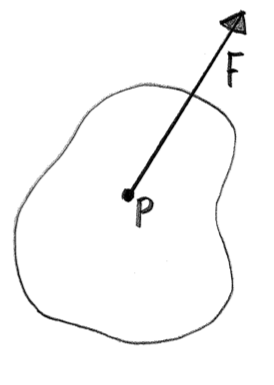
\includegraphics[width=40mm]{./images/physics_work_a.png}}
%   \end{minipage}
%   %\hspace{0.5cm}
%   \begin{minipage}[b]{0.3\linewidth}
%     \centering
%     \subfloat[]{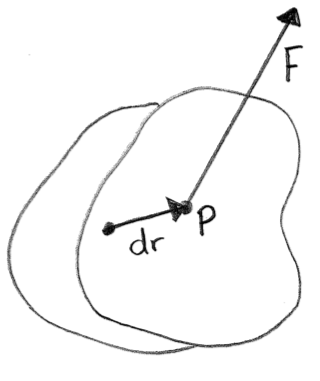
\includegraphics[width=40mm]{./images/physics_work_b.png}}
%   \end{minipage}
%   %\hspace{0.5cm}
%   \begin{minipage}[b]{0.3\linewidth}
%     \centering
%     \subfloat[]{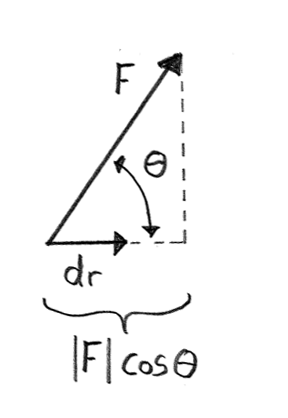
\includegraphics[width=40mm]{./images/physics_work_c.png}}
%   \end{minipage}
% \end{figure}
  
\begin{figure}
  \centering
  \subfloat[A force $f$ acting on an object]{
    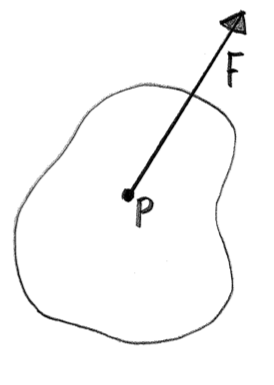
\includegraphics[width=4cm]{./images/physics_work_a.png}
    \label{fig:worka}
  }
  \subfloat[A displacement $dr$ of $P$]{
    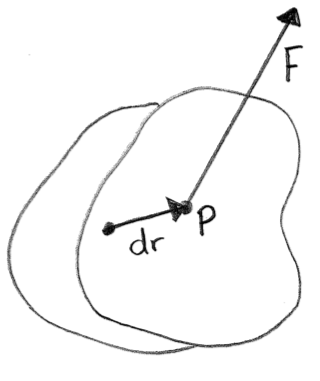
\includegraphics[width=4.5cm]{./images/physics_work_b.png}
    \label{fig:workb}
  }
  \subfloat[$dW=(|f|cos \phi)|dr|$]{
    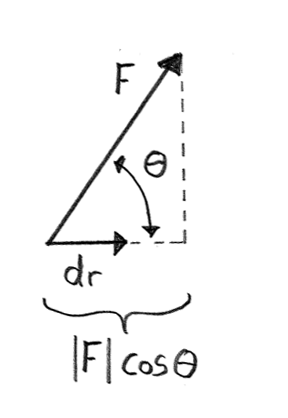
\includegraphics[width=4.3cm]{./images/physics_work_c.png}
    \label{fig:workc}
  }
  \caption{Illustration of work.}
  \label{fig:work}
\end{figure}


% \subsubsection{Virtual Displacement and Virtual Work}
% \label{sec:virtual-work}
% When using the term \defit{virtual} in the context of physics, it
% refers to an imagined scenario. For example: We can talk about a virtual
% displacement of an object event though the object cannot move. The
% virtual displacement is not applied to the object but we can use
% this imaginary displacement to do calculations on the object. In
% mathematical notation virtual is denoted $\delta$. Virtual
% displacement is denoted $\delta r$.
% %
% Virtual work is defined in terms of virtual displacement, and is
% therefore also an imaginary thing.

% \begin{equation}
% \delta W = f \cdot \delta r
% \end{equation}

% Virtual work is used to analyse complete structures via the
% conservation law: \defit{principle of virtual work} to be introduced
% in section \vref{sec:principle-of-virtual-work}
% \citebook{page~558-561}{book:static-mechanics}.

\subsection{Energy}
% enhed J
Although work and \defit{energy} are related and both are measured in
Joule (J), they are not entirely equal concepts. Work refers to a force
acting over a distance. Energy on the other hand is
used when referring to the amount stored or produced by an
object. We use two concepts to describe an object's energy: \defit{Kinetic
  energy} and \defit{potential energy}. 

\subsubsection{Kinetic Energy}
\defit{Kinetic energy} is the energy of motion. Whenever an object moves it
possesses kinetic energy. The amount of kinetic energy within an object
with mass $m$ and velocity $v$ is defined as the work needed to
accelerate the mass $m$ from rest to velocity $v$. The object maintains
its kinetic energy as long as the velocity is constant. If the
velocity increases or decreases so does the kinetic energy. It would
require the same amount of work to decelerate an object to rest, as it
took to accelerate it to velocity $v$. The force required to
decelerate the object has to be in the opposite
direction. The kinetic energy $E_K$ of an object is defined by
\citebook{page~164-165}{book:uni-physics}:

\begin{equation}
E_K = \frac{1}{2} m v^2
\end{equation}

Kinetic energy is related to work by the \defit{work-energy theorem},
which states that work equals the change in kinetic energy
\citebook{page~170}{book:uni-physics}:

\begin{equation}
W = E_K^1 - E_K^0 = \Delta E_K
\end{equation}

\subsubsection{Potential Energy}
\defit{Potential energy}, denoted $E_U$, is the energy stored within a
physical system. An
object can possess potential energy as a result of its position. If for
example a heavy weight is elevated and held above the ground it
possesses potential energy. The energy stored has the potential to be
converted into a different form of energy, e.g. kinetic
energy. Compressing a spring is another way of storing potential
energy within an object. If the force compressing the spring is
removed the spring's restoring force will make it return to its
original position. Potential energy exists when an object 
is displaced and there are forces acting towards bringing
the object back to its original position. 
%

\subsubsection{Conservative and Non-conservative Systems}
When kinetic energy can be converted to potential energy, and back
again, we say that there is a two-way conversion of energy. Systems
with the two-way conversion property are \defit{conservative systems},
those without are \defit{non-conservative systems}. A system where
energy is turned into heat is an example of the latter
\citebook{page~209-210}{book:uni-physics}.
Conservative systems are isolated and have the property that energy
does not dissipate.

\subsubsection{Conservation of Mechanical Energy}
\label{sec:conser-of-me}
When dealing with a conservative system the total amount of
energy is referred to as the mechanical energy ($E_M$), and is defined
by:

\begin{equation}
\label{eq:mech-energy}
E_M = E_K + E_U
\end{equation}

In a conservative system no energy dissipates therefore the mechanical
energy within the system is constant.
Kinetic energy can be stored by converting it to potential energy. The
classic example is: When throwing a ball upwards, kinetic energy is
converted into potential energy on the way up. On the way down the
opposite happens. The relation that makes this possible is called 
\defit{conservation of mechanical energy} and is a direct consequence
of equation \eqref{eq:mech-energy} for a conservative system
\citebook{page~196}{book:uni-physics}:
%
If we consider an object that is deformed, it has an initial state
(state 0), and a deformed state (state 1). In both states the energy
can be calculated as:

\begin{equation}
E_M^0 = E_K^0 + E_U^0 \qquad E_M^1 = E_K^1 + E_U^1
\end{equation}

if the system is conservative, we know that:

\begin{equation}
\label{eq:external_work_equals_internal_energy}
\begin{aligned}
E_M^0 &= E_M^1  \qquad \Leftrightarrow \\
E_K^0 + E_U^0 &= E_K^1 + E_U^1 \qquad \Leftrightarrow \\
E_K^0 - E_K^1 &= E_U^1 - E_U^0  \qquad \Leftrightarrow \\
- (E_K^1 - E_K^0) &= E_U^1 - E_U^0  \qquad \Leftrightarrow \\
- W &= E_U^1 - E_U^0  \qquad \Leftrightarrow \\
- W &= \Delta E_U
\end{aligned}
\end{equation}

by setting the initial potential energy
$E_U^0$ to zero, we obtain:

\begin{equation}
\label{eq:EW}
E_U^1 = -W 
\end{equation}

% \subsubsection{Principle of Virtual Work for Conservative Forces}
% \label{sec:principle-of-virtual-work}
% Work done by a conservative force can be expressed in terms of its
% potential energy. It can be expressed by using the definition of
% mechanical equilibrium as defined in definition
% \vref{mechanical-equilibrium}.
% %
% The definition states that change in total virtual potential energy is
% zero: $\delta \Delta E_U = 0$.
% %
% And because the mechanical energy $E_M = E_K + E_U = 0$, we know that
% $E_U=-E_K$. So the change in potential energy must be the negative
% change of kinetic energy: $\Delta E_U = - \Delta E_K$. As $\Delta
% E_K = W$, we have that $\delta \Delta E_U = - \delta W = 0$.
% %
% In effect this means that the total virtual work must be zero. That
% is, the work done by the internal forces plus the work done by the external
% forces must be zero, so adding up the work done by the internal forces
% with the work done by the external forces this becomes the
% \defit{principle of virtual work}:

% \begin{equation}
% \label{eq:principle_of_virtual_work}
%   \mbox{total virtual work} = \mbox{internal virtual work} +
%   \mbox{external virtual work} = 0
% \end{equation}
% \begin{equation}
%   \mbox{internal virtual work} = - \mbox{external virtual work}
% \end{equation}

% The principle of virtual work has an important property, it can be
% applied to entire structures. This means that structures composed of
% elements can be analysed \citebook{page~560-561}{book:static-mechanics}.
% A continuum consists of infinitesimal
% elements, therefore the principle of virtual work applies when
% analysing continuums.


\section{Continuum Mechanics}
\label{sec:continuum}
In continuum mechanics we assume that the substance of a body is a
continuously distributed matter, that is distributed
throughout and completely fills the space it occupies. We also assume
that the substance is \defit{homogeneous}, that is, the entire body
consists of the same material. Continuum
mechanics ignores the fact that matter is not continuous at the level
of atoms. By ignoring this we can approximate physical quantities, 
such as energy and work, at the infinitesimal limit.

\subsection{Continuum}
Continuum as a concept describes a material as a fixed region of
space. This region forms the geometrical state of a body. We imagine the
region completely covered by a set of infinitesimal volumetric
elements, called \defit{particles}. The position of all particles at a
time $t$ is called a \defit{configuration}.
%
A particular configuration is chosen as the \defit{reference
  configuration} and each particle in the reference configuration is
identified by the position vector $X$. The reference configuration is often
chosen as the configuration at time $t=0$, where the body
is in an undeformed state and at rest
\citebook{page~4}{book:continuum-mechanics}.

%\layoutpb

\begin{figure}
  \centering
  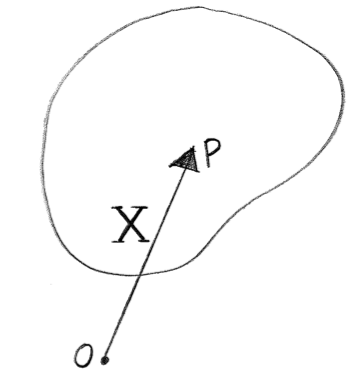
\includegraphics[width=4.5cm]{./images/physics_continuum_body.png}
\caption{A continuum body.}
\label{fig:continuum}
\end{figure}

% \begin{figure}
%   \centering
%   \includegraphics[width=6cm]{./images/wiki-Continuum_body.png}
% \caption{A continuum body}
% \label{fig:continuum}
% \end{figure}

The components of $X$ in the chosen reference frame are referred to as
the \defit{material coordinates}. We say that the particle $P$ occupies
the place $X$ as illustrated in figure \vref{fig:continuum}. Suppose
that the region covered by the body at
\defit{reference time} $t=0$ is $R_0$. If the body moves and at
time $t$ occupies $R$, then we describe this configuration in
relation to the reference configuration by \defit{spatial coordinates}
$x$. 
This scenario is illustrated in figure \vref{fig:displacement}.
The spatial coordinates are the material coordinates plus a
displacement: $x = X + u$, where $u$ is referred to as the
\defit{displacement vector}.
Spatial coordinates can also be calculated as a function $f$ of the
reference configuration and time: $x = f(X,t)$ 
\citebook{page~33-35}{book:continuum-mechanics-anthony}.
Note that by the definition of material and spatial coordinates,
there has to be a one-to-one correspondence between \defit{material
  points} and \defit{spatial points}.

\begin{figure}
  \centering
  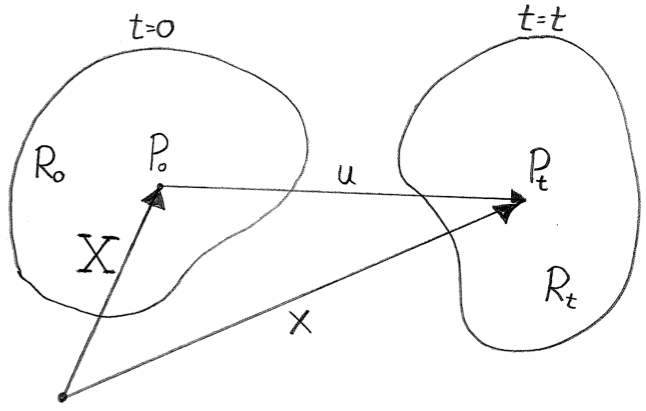
\includegraphics[width=8cm]{./images/physics_displacement.png}
\caption{Displacement of a continuum.}
\label{fig:displacement}
\end{figure}

% \begin{figure}
%   \centering
%   \includegraphics[width=12cm]{./images/wiki-Displacement_of_a_continuum.png}
% \caption{A displacement}
% \label{fig:displacement}
% \end{figure}

\subsection{Deformation}
\label{sec:deformation}
If two configurations of a body are not the same,
one or more of the particles have been displaced. A
\defit{displacement} can be divided into two distinct components: a
\defit{rigid body displacement} and a \defit{deformation}.
%
The difference being whether or not particles have moved in
relation to each other. In a rigid body displacement the relative
inter-particle distances are preserved. In a deformation they are not.

% \begin{figure}
%   \centering
%   \includegraphics[width=8cm]{./images/solid-mechanics-c2-1.png}
% \caption{A deformation}
% \label{fig:deformation}
% \end{figure}

\begin{figure}
  \centering
  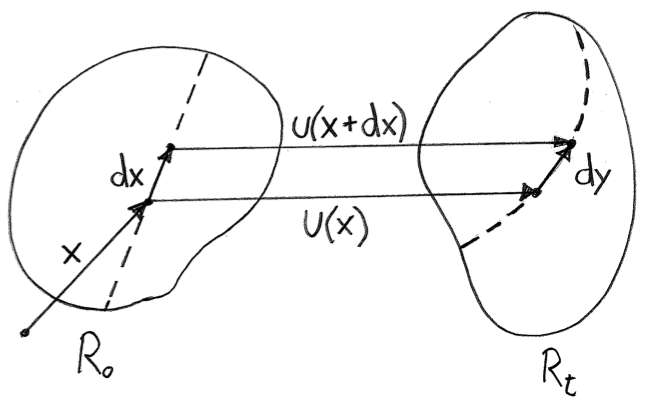
\includegraphics[width=8cm]{./images/physics_deformation_of_line.png}
\caption{Deformation of an infinitesimal line segment.}
\label{fig:deformation_of_line}
\end{figure}

Consider the straight line through the undeformed configuration $R_0$ as
illustrated in figure \vref{fig:deformation_of_line}. After the body
has undergone a deformation the straight line has been mapped to a
smooth curve as illustrated in the deformed configuration $R_t$. Somehow we
would like to represent the line or fiber deformation that takes
place. Focus attention on the line segment $dx$ and imagine that the
length of the line segment is much shorter than the radius of
curvature. The small line segment is straight in the undeformed
configuration and very close to straight in the deformed
configuration. By decreasing the length of the line segments we
improve the approximation of the curvature. This way we can describe
even complex deformations of a body since it is reasonable to neglect
curved material fibers as long as we only consider infinitesimal line
segments. The infinitesimal line segments $dx$ and $dy$ are related by
the ratio: $\frac{dy}{dx}$
\citebook{section~2.1.2}{book:solid-mechanics}.
% the following is directly copied from book:s% olid-mechanics
% \{ To illustrate deformation, imagine drawing a straight line on the
% undeformed configuration as shown in figure
% \vref{fig:deformation-of-line}. The line would be mapped to a smooth
% curve in the deformed configuration. However suppose we focus
% attention on a line segment $dx$, much shorter than the radius of the
% curvature of this curve. The segment would be straight in
% the undeformed configuration, and would also be (almost) straight in
% the deformed configuration. Thus, no matter how complex a deformation
% we impose on a body, infinitesimal line segments are merely
% stretched and rotated by a deformation. The infinitesimal line segments
% $dx$ and $dy$ are related by the ratio: $\frac{dy}{dx}$
% \citebook{section~2.1.2}{book:solid-mechanics}.}
% % the above is directly copied from book:solid
%-machanics
If this ratio is $1$ the material is undeformed, between $0$ and
$1$ it is compressed and if above $1$ it is stretched.
%The concept of stretch and compression
%is illustrated in figure \vref{fig:tension}.
%

% \begin{figure}
%   \centering
%   \subfloat[Stretching]{
%     \includegraphics[width=6cm]{./images/uni-physics-p338-f11-9.png}
%     \label{fig:stretching}
%   }
%   \subfloat[Compression]{
%     \includegraphics[width=6cm]{./images/uni-physics-p339-f11-11.png}
%     \label{fig:compression}
%   }
%   \caption{Stretching contra compression}
%   \label{fig:tension}
% \end{figure}

\subsection{Strain}
\label{sec:physics_strain}
%
Strain is a measure of deformation. Strain represents the amount of
stretch or compression by the relative distance between two particles
in the material body. It is a dimensionless quantity, which can be
expressed as a decimal fraction, or a percentage.
%
In comparison with the ratio $\frac{dy}{dx}$ from section
\vref{sec:deformation}: A strain measure of zero means no deformation,
below or above represents compression or stretching respectively.
%
Strain can be decomposed into \defit{normal strain} and
\defit{shearing strain}.

%To better understand strain, we can divide it into two distinct
%components: Normal or tensile strain and shearing strain.

\subsubsection{Normal Strain}
Normal strain occurs when forces acting parallel to the axes of the
reference frame pull equally throughout the body. Normal strain has
the property of scaling the body in the axial directions. Figure
\vref{fig:normalstrain} illustrates normal strain in one
dimension. Here two external forces pull in opposite
directions on a body hereby stretching it.

\begin{figure}
  \centering
  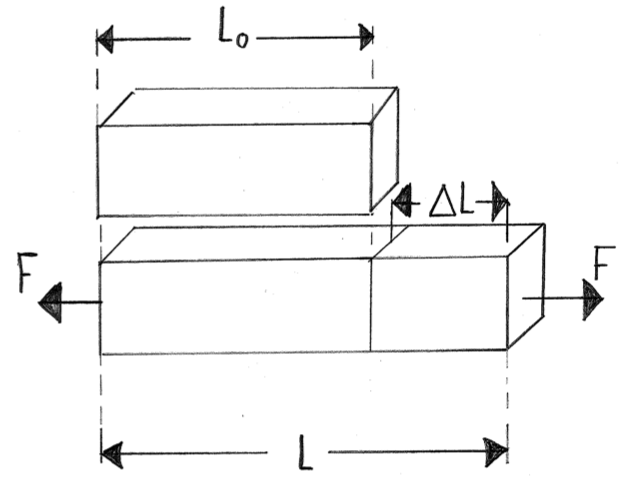
\includegraphics[width=6cm]{./images/physics_normalstrain.png}
\caption{Normal strain.}
\label{fig:normalstrain}
\end{figure}

For the simple case of a body axially loaded,
the normal strain will be uniformly distributed throughout the body
and can be obtained by dividing the displacement (how much the body is
stretched) by the initial length of the body.
%Normal strain is defined to be the displacement (how much the body
%is stretched) divided by the length of the body.

\begin{equation}
\mbox{normal strain: } \frac{l-l_0}{l_0} = \frac{\Delta l}{l_0}
\end{equation}

In general strain is not distributed uniformly over the entire
body, therefore we define strain at a specific point within the
body. Because continuum mechanics assumes strain to be continuous,
differential calculus is used to define strain at any point.
In three dimensions, we have a normal strain component
for each direction in the reference frame. Written out as individual
components this becomes: \citebook{page~659}{book:fem-engineers}

\begin{equation}
\label{eq:individual-normal-strain}
\varepsilon_x = \frac{\partial u_x}{\partial x} \hspace{10 mm}
\varepsilon_y = \frac{\partial u_y}{\partial y} \hspace{10 mm}
\varepsilon_z = \frac{\partial u_z}{\partial z}
\end{equation}

were $u$ is the displacement vector with components $u_x$, $u_y$ and
$u_z$ being the displacement along the $x$, $y$ and $z$ axis of the
reference frame, respectively. Normal strain can be represented on
vector form as:
$\varepsilon = [ \varepsilon_x, \ \varepsilon_y, \ \varepsilon_z ]^T$.

\subsubsection{Shearing Strain}
Shearing strain occurs when the forces are not aligned with the axes
of the reference frame or if they are not uniformly distributed over
the body. This results in distortion of the body's shape as
illustrated in figure \vref{fig:shear-strain}.

% \begin{figure}
%   \centering
%   %\includegraphics[width=6cm]{./images/uni-physics-p343-f11-17.png}
%   \includegraphics[width=14cm]{./images/deformation-shearing-strain.png}
% \caption{Shear strain}
% \label{fig:shearstrain}
% \end{figure}

\begin{figure}
  \centering
  \subfloat[Shearing strain in one direction.]{
    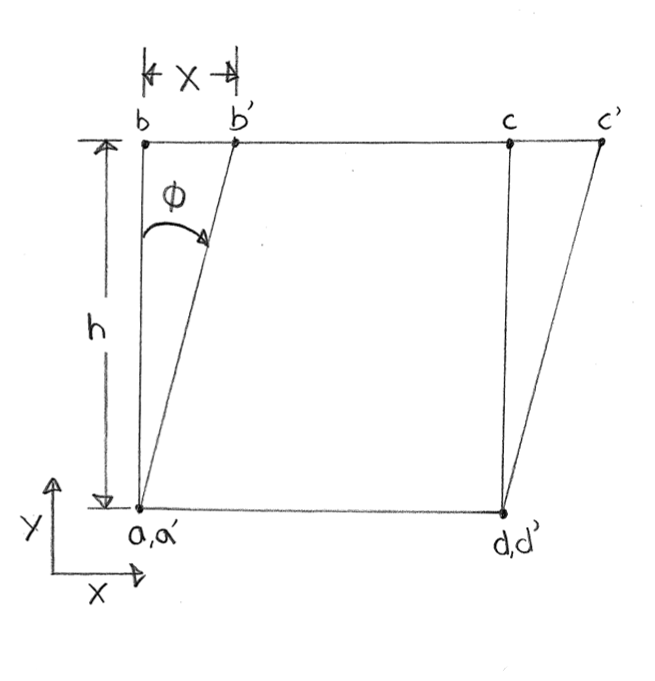
\includegraphics[width=7cm]{./images/physics_shearing_strain_a.png}
    \label{fig:shearing-strain-one-direction}
  }
  \subfloat[Shearing strain in two directions.]{
    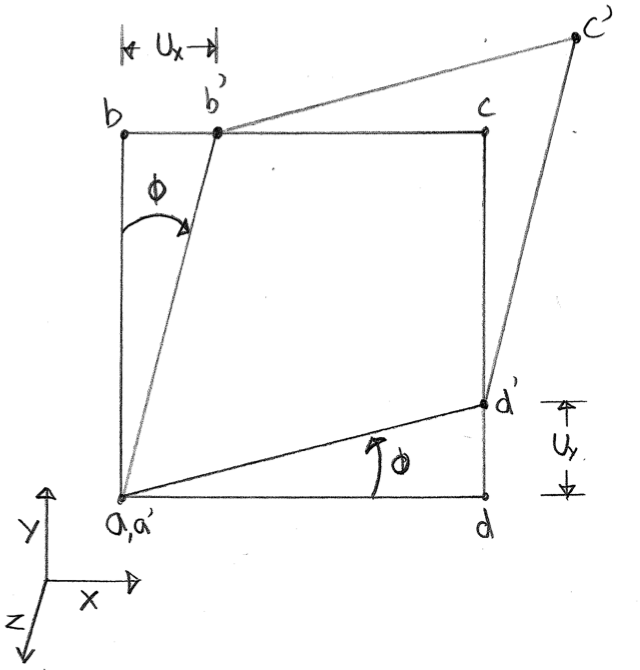
\includegraphics[width=7cm]{./images/physics_shearing_strain_b.png}
    \label{fig:shearing-strain-two-directions}
  }
  \caption{Shearing strain.}
  \label{fig:shear-strain}
\end{figure}

Shear strain is defined as the ratio of the displacement $x$ of the corner
$b$ to the transverse dimension $h$ \citebook{page~343}{book:uni-physics}:

\begin{equation}
\mbox{shear strain: } \frac{x}{h} = tan \phi
\end{equation}

Figure \vref{fig:shearing-strain-one-direction} illustrates basic
shearing strain in one direction. In three dimensions we are
interested in defining the resulting shear strain between
planes. Figure \vref{fig:shearing-strain-two-directions} illustrates
the distortion from shear strain in two directions. To measure the
resulting shear strain between the $xz$-plane and the $yz$-plane the
two individual shearing strains are added.
%
The individual components of the shearing strain in three dimensions are
\citebook{page~7}{book:theory-of-elasticity}:

\begin{equation}
\label{eq:individual-shear-strain}
  \gamma_{xy} = \frac{\partial u_x}{\partial y} +
  \frac{\partial u_y}{\partial x} \hspace{10 mm}
  \gamma_{xz} = \frac{\partial u_x}{\partial z} +
  \frac{\partial u_z}{\partial x} \hspace{10 mm}
  \gamma_{yz} = \frac{\partial u_y}{\partial z} +
  \frac{\partial u_z}{\partial y}
\end{equation}

where $u_x$, $u_y$ and $u_z$ are the axial displacements along the $x$, $y$
and $z$ axis, respectively. Shearing strain can be represented on vector
form as: $\gamma = [ \gamma_{xy}, \ \gamma_{xz}, \ \gamma_{yz} ]^T$.\\

% Applying shear strains along two axes is the same as applying the
% total shear strain along one axis when only measuring the total amount
% of shearing in the given plane. 
% The two distorted squares illustrated in figure \vref{fig:shear-strain}
% are equivalent; the only difference is that the one to 
% the right is translated and rotated slightly.
% Since we are only interested in measuring the resulting shear in each
% plane, and not interested in the resulting orientation of the square,
% we add the two axial shear strains together to obtain
% the equations \eqref{eq:individual-shear-strain}.

%$\frac{\partial u_x}{\partial y}$ represents
%the shear strain in the $x$ direction and $\frac{\partial
%  u_y}{\partial x}$ is in the $y$ direction. 


%internal forces (static p. 448)
\subsection{Internal Forces}
\label{sec:internal-forces}
Internal forces only exist inside an object, where one part of an
object is subjected to forces by another part of the same object
\citebook{page~79}{book:static-mechanics}. 
Internal forces can be experienced simply by stretching a rubber
band. When stretching a rubber band the external force, responsible for
the stretching, induces internal forces. When the external force is
released the rubber band returns to its original shape
hereby releasing the internal forces as well. The way a body behaves
depends on its material properties. How different materials behave is
elaborated in section \vref{mechanical-properties}, but first stress
is introduced as this is a representation of the internal forces.

\subsection{Stress}
\label{sec:physics_stress}
Stress is a measure of the average amount of force exerted per unit
area ($N$/$m^2$). It is a measure of the intensity of the total
internal forces acting within a body across imaginary internal
surfaces, as a reaction to externally applied forces.
%In
%general, stress is expressed as a force $f$ acting over area $A$: 

\begin{equation}
\mbox{stress} = \frac{f}{A}
\end{equation}


As with strain, stress can be decomposed into two separate components:
\defit{normal stress} and \defit{shearing stress}.
Consider an infinitesimal cubic element with
edges parallel to the axe as illustrated in figure
\vref{fig:stress_box}.

%As with strain, stress can be decomposed into normal ($\sigma$) and
%shearing stress ($\tau$).

\begin{figure}
  \centering
  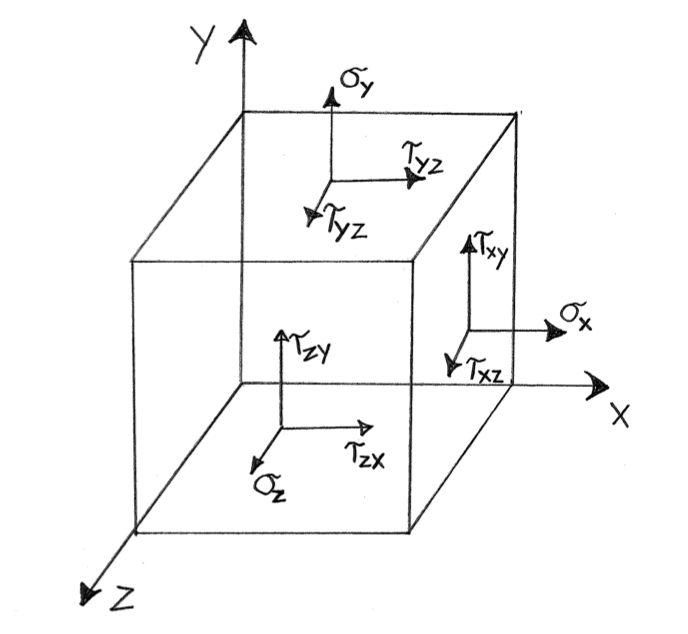
\includegraphics[width=8cm]{./images/physics_stress_box.png}
\caption{Stress in three dimensions.}
\label{fig:stress_box}
\end{figure}

The components of normal stress are denoted $\sigma_x$,
$\sigma_y$ and $\sigma_z$, one for each axial stress acting
perpendicular to a body face. Normal stress is either tension or
compression, often causing change in volume. Shearing stress is
denoted $\tau_{xy}$, $\tau_{yz}$ and $\tau_{zx}$, each
acting parallel or tangential to a body face causing it
to deform without particular volume change.
% Figure \vref{fig:stress-box} shows the notation used to define stress in three
% dimensions. The components of normal stress are denoted $\sigma_x$,
% $\sigma_y$ and $\sigma_z$, one for each axial stress.
% %
% Shear stress is denoted $\tau_{xy}$,
% $\tau_{yz}$ and $\tau_{zx}$. 
The first letter in the double subscript
indicates the \defit{plane} in which the stress acts, whereas the second
subscript indicates in which \defit{direction} the stress
acts.
%the coordinate direction which is normal to the plane in which the stress
%acts; the second subscript indicates the coordinate direction
%in which the stress acts. 
For example $\tau_{xy}$ has $x$ as its first
subscript therefore the stress acts in the $yz$-plane because the
direction $x$ is a normal to this plane. The second subscript
is $y$ indicting the actual stress direction.
%
We assume equilibrium of the element's volume, therefore $\tau_{xy}$
must be equal to $\tau_{yx}$ or else the element would not be at
rest. This means we only need three shear stress components since
$\tau_{xy} = \tau_{yx}$, $\tau_{yz} = \tau_{zy}$, and $\tau_{zx} =
\tau_{xz}$.
%Only three components of shear stress are
%needed, as only these three are independent ($\tau_{xy} = \tau_{yx}$,
%$\tau_{yz} = \tau_{zy}$ and $\tau_{zx} = \tau_{xz}$).
Altogether we only need the six independent quantities $\sigma_x$,
$\sigma_y$, $\sigma_z$, $\tau_{xy}$, $\tau_{yz}$ and $\tau_{zx}$ to completely
describe the state of stress at a given point in the
continuum \citebook{page~658}{book:fem-engineers}.
%
When considering stress in three dimensions we refer to the measure as
a force per volume, rather then the individual components as force per
area. The normal stress can be represented on vector form as
$\sigma = [ \sigma_{x}, \ \sigma_{y}, \ \sigma_{z} ]^T$ and the
sharing stress as 
$\tau = [ \tau_{xy}, \ \tau_{xz}, \ \tau_{yz} ]^T$.

\subsection{Strain Energy}
The potential energy stored within a deformed body is called \defit{strain
  energy}. Strain energy is calculated the same way, we calculate
work, but instead of relating force and displacement we use the stress
and strain induced in the body. The body's internal potential strain
energy is calculated as:

\begin{equation}
\label{eq:strain_energy}
E_S = 
\int_{V} \varepsilon \cdot \sigma \ dV +
\int_{V} \gamma \cdot \tau \ dV
\end{equation}

where the strain and stress vectors dotted and integrated over the
volume $V$ yields the internal potential strain energy. The integral
insures that the internal forces are distributed uniformly throughout
the volume \citebook{page~224}{book:applied_math}.
%
Because stress is a force per volume measure, the strain energy is
also a force per volume measure.

\subsection{Strain Energy Density}
The \defit{strain energy density} $dE_S$, is the strain energy
per unit volume, which can be obtained by
\citebook{page~625}{book:tim-mom}:

\begin{equation}
\label{eq:strain_energy_density}
dE_S = 
\int_0^\varepsilon \sigma \ d \varepsilon  +
\int_0^\gamma \tau \ d \gamma 
\end{equation}

and when stress-strain curves are introduced in section
\vref{sec:sscs}, this constitutes the area below such a curve. Strain
energy and strain energy density are directly related by the following
equation:

\begin{equation}
\label{eq:strain_energy_density_integral}
E_S = 
\int_V dE_S \ dV
\end{equation}

%\subsection{Strain energy density function}
%relates the strain energy density of a material to the deformation
%gradient.


% \subsection{Equilibrium for a Continuum}
% As described in section \vref{sec:principle-of-virtual-work},
% equilibrium for a continuum is defined in terms of the
% principle of virtual work. This principle states that: $\mbox{internal
%   virtual work} = -\mbox{external virtual work}$. To use this
% definition on a continuum we need to know how to calculate the
% internal and external virtual work. The internal virtual work for a
% continuum is defined as:

% \begin{equation}
% \label{eq:internal_virtual_work}
%   \mbox{internal virtual work:}
%   \int_{V} \delta \varepsilon \cdot \sigma \ dV +
%   \int_{V} \delta \gamma \cdot \tau \ dV
% \end{equation}

% where the transpose of the virtual normal strain vector $\varepsilon$ multiplied by
% the normal stress vector and integrated over the volume $V$ yields
% the internal virtual work. The integral insures that the internal
% forces are distributed uniformly throughout the volume
% \citebook{page~224}{book:applied_math}.

% The external virtual work is defined to be: $\mbox{virtual surface work} +
% \mbox{virtual body work}$. Forces acting upon the body (volume) are denoted
% $f_V$ and traction (surface forces) $f_S$, $\delta u$ is the virtual
% displacement vector, $V$ the volume and $S$ is the surface. The virtual
% work is calculated as described in section \vref{sec:virtual-work}
% and integrated over the volume and surface respectively:

% \begin{equation}
%   \mbox{virtual surface work:} \int_{S} \delta u \cdot f_S \ dS
%   \qquad
%   \mbox{virtual body work:} \int_{V} \delta u \cdot f_V \ dV 
% \end{equation}

% Substituting these definitions into the principle of
% virtual work, we obtain:

% \begin{equation}
%   \label{eq:povw}
%   \int_{V} \delta \varepsilon \cdot \sigma \ dV +
%   \int_{V} \delta \gamma \cdot \tau \ dV =
%   \int_{S} \delta u \cdot f_S \ dS +
%   \int_{V} \delta u \cdot f_V \ dV
% \end{equation}

% Consider equation \eqref{eq:povw}, when external forces are applied,
% the body reacts by either adjusting the virtual displacement or the
% level of stress.

\subsection{Equilibrium for a Continuum}
\label{sec:equilibrium-for-a-continuum}
As described in section \vref{sec:equilibrium-for-deobj}, equilibrium
for a deformable object is defined in terms of energy. Here we will
specify this definition for a continuum. Recall from section
\vref{sec:conser-of-me} that when an object has changed shape we
consider two states of the object and their energy relation. Equation
\eqref{eq:EW} is repeated below, it relates the
change in potential energy to the work done by kinetic
energy. Equilibrium for a continuum is precisely this, the relation
between the work done by external force, and the resulting internal
force measured as potential energy.

\begin{equation*}
- W = \Delta E_U
\end{equation*}

As normally done we set the initial potential energy $E_U^0 = 0$,
which means that the equation becomes: $- W = E_U^1$. The internal
potential energy is the strain energy for a continuum and is defined
in equation \eqref{eq:strain_energy} as:

\begin{equation*}
  E_S = \int_{V} \varepsilon \cdot \sigma \ dV +
  \int_{V} \gamma \cdot \tau \ dV
\end{equation*}

The work done by the external forces is defined to be:
$\mbox{surface work} + \mbox{body work}$.
Forces acting upon the body (volume) are denoted $f_V$ and traction
(surface forces) $f_S$, $u$ is the displacement vector, $V$ the volume
and $S$ is the surface. The work is calculated by integrating force times
displacement over the volume and surface, as described in section
\vref{sec:work}.

\begin{equation}
  \mbox{surface work:} \int_{S} u \cdot f_S \ dS
  \qquad
  \mbox{body work:} \int_{V} u \cdot f_V \ dV 
\end{equation}

A surface integral can be converted into a volume integral
using the Gauss divergence theorem. By doing this the total external
work can be expressed as
\citebook{page~49}{book:continuum-mechanics-mase}:

\begin{equation}
  \label{eq:external-work}
  \mbox{external work:}
  \int_{V} u \cdot f_V \ dV
\end{equation}

Substituting these definitions into the equation: $ -W= E_P^1$, we obtain:

\begin{equation}
  \label{eq:pompe}
  - ( \int_{V} u \cdot f_V \ dV ) =
  ( \int_{V} \varepsilon \cdot \sigma \ dV +
  \int_{V} \gamma \cdot \tau \ dV )
\end{equation}

Consider equation \eqref{eq:pompe}, when external forces are applied,
the body reacts by either adjusting the displacement or the level of
internal energy.

\section{Mechanical Properties}
\label{mechanical-properties}
We will now elaborate on how stress and strain is related. Mechanical
properties of a material describe how stress and 
strain are related in the given material.
%
As the stress and strain increases with the external force applied,
the material behaviour changes.
Mechanical properties are theoretically divided into different
phases based on how the material behaves. The first phase represents  
\defit{elastic deformation}, here the material absorbs the forces and
stores them as stress and strain. The second phase represents
\defit{plastic deformation}, during this phase the internal structures
of the material change permanently. If the amount of stress and
strain exceeds the point of \defit{fracture} the material will collapse.
Elastic deformation is reversible, but the other deformation types are not.
\citebook{page~344-345}{book:uni-physics}

% When a body is applied external force until it breaks, the material
% passes through different types for deformation. 

% In the first phase,
% denoted \defit{elastic deformation}, the material absorbs the forces and
% stores them as stress and strain. At some point the material is
% subjected to so much external force that it starts to break.
% In this second phase, termed \defit{plastic deformation}, the internal
% structure or property of the material changes. At some point the
% material cannot withstand anymore forces and it fractures. 

\subsection{Stress-strain Curves}
\label{sec:sscs}
To visualize how a material goes through the different
types of deformation, we look at stress-strain curves. A stress-strain
curve is a graph where measurements of stress as a function of
strain, are plotted. The graph should be interpreted as follows: When
moving away from origin along the $x$ axis, the material gets more and
more stretched (or compressed) depending on the direction. Normally
the stress-strain curve only includes stretch, which is positive along
the $x$ axis.
%
Isotopic materials yield the same stress-strain curve in
any direction, therefore only one stress-strain curve is needed. To
describe an anisotropic material more than one stress-strain curve is
needed.
%
The stress-strain curves in figure \vref{fig:stress-starin-overview},
show an overview of how to interpret the curves. Figure
\ref{fig:ssc-phaces} illustrates the different phases and figure
\ref{fig:ssc-points} the names of the transition points between the
phases. The transition point between linear and non-linear elasticity
is called \defit{proportional limit}. Between elastic and
plastic deformation it is called \defit{yield strength}, and the
material will break when reaching the \defit{fracture point}.
The maximum amount of stress during plastic deformation is called the
\defit{ultimate strength} limit.

\begin{figure}
  \centering
  \subfloat[Phases.]{
    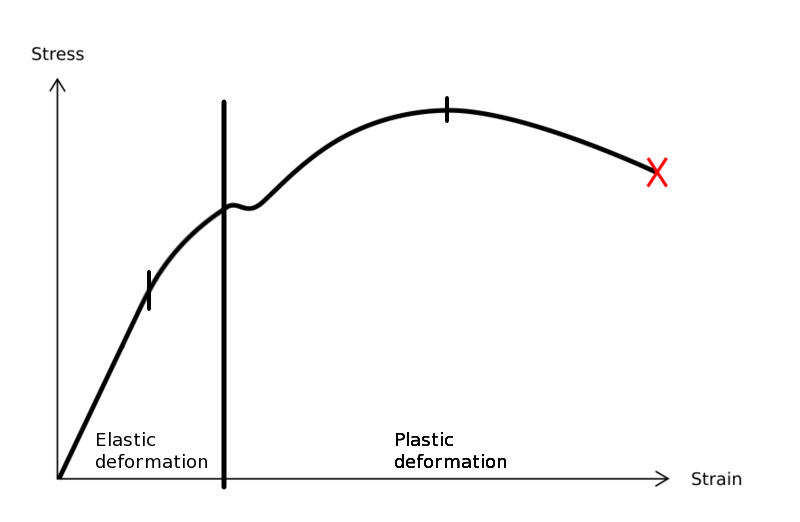
\includegraphics[width=7.5cm]{./images/physics_ssc_phases.png}
    \label{fig:ssc-phaces}
  }
  \subfloat[Points.]{
    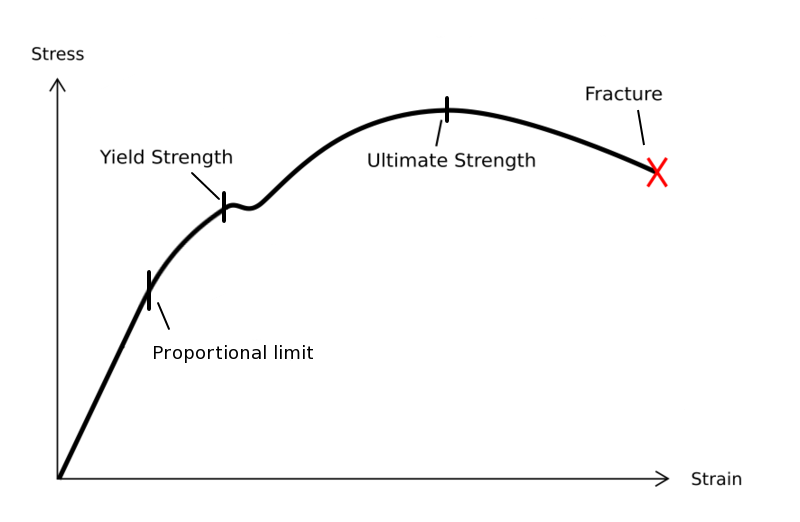
\includegraphics[width=7.5cm]{./images/physics_ssc_points.png}
    \label{fig:ssc-points}
  }
  \caption{Stress-strain curves overview.}
  \label{fig:stress-starin-overview}
\end{figure}

\subsection{Elastic Deformation}
\label{sec:elastic-deformation}
Elastic deformation or elasticity is the physical property of a
material when it deforms due to external forces applied, but returns to its
original shape when the forces are removed. The material returns to
the original form because the applied forces are stored as
stress and strain. The relation between stress and strain under
elastic deformation can be either linear, non-linear or both depending
on the material properties. \defit{Linear elasticity} is when strain
is directly proportional to stress. \defit{Non-linear elasticity} is
when the relationship between strain and stress is more complex and
can be approximated by a non-linear function. A material with both
properties is illustrated in figure \vref{fig:ssc-elasticity}.

\begin{figure}
  \centering
  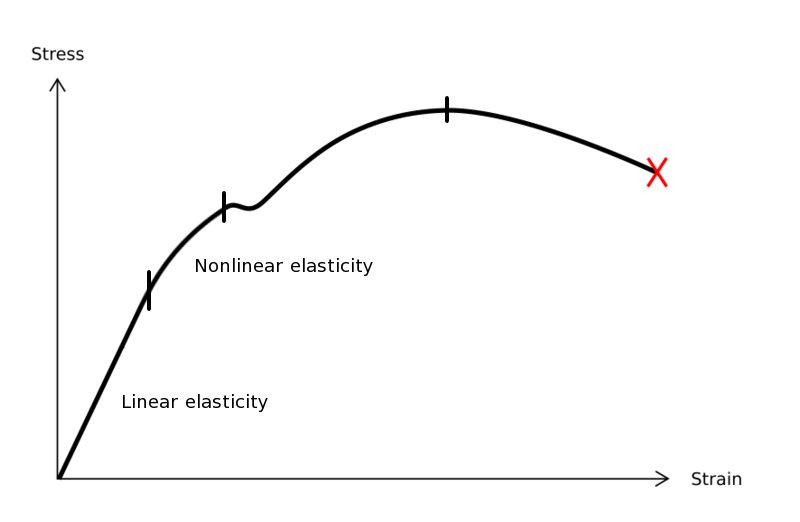
\includegraphics[width=7.5cm]{./images/physics_ssc_elasticity.png}
\caption{Stress-strain curve illustrating elastic deformation.}
\label{fig:ssc-elasticity}
\end{figure}

%Elastic deformation is instantaneous, which means that if we increase
%the strain we get an immediately change in stress.
Elastic deformation is
completely reversible. If the stress is reduced to its former value
the strain falls back to the original level
\citebook{page~183}{book:material-science}.

\subsection{Plastic Deformation}
\defit{Plastic deformation}, also known as \defit{plastic flow}, is an
irreversible deformation, which means that the body will not return to
its original configuration when the external forces are released. When
the amount of external forces exceeds the yield strength the plastic
deformation phase takes over.
%
Plastic deformation changes the rest shape of a material, by
changing its structure at the level of atoms. Atoms
are bound in a grid structure. This grid structure is
permanently changed by \defit{dislocations} along \defit{slip planes}.
\citebook{page~191-205}{book:material-science}.
%
An important property of plastic deformation is that it preserves the
volume of the material.
%
An example of a plastic deformable material is metal. If metal is
bent, the material's rest shape is permanently changed.
%
The stress-strain curve in figure \vref{fig:ssc-restshape} shows a
material that has gone through linear elastic deformation (stage 1-2),
non-linear elastic deformation (stage 2-3) and plastic deformation (3
and onwards). If at a point (4), the external forces are 
released, the material has obtained a permanent deformation and
therefore a new rest shape. The material returns to the new rest
shape via the dotted line.
%
If the material is, once more, subjected to external forces, the
deformation of the material follows the dotted line until the point of
yield strength is reached, and continues into plastic deformation if
enough forces are applied \citebook{page~159}{book:continuum-mechanics}.

\begin{figure}
  \centering
  \subfloat[Plastic deformation.]{
    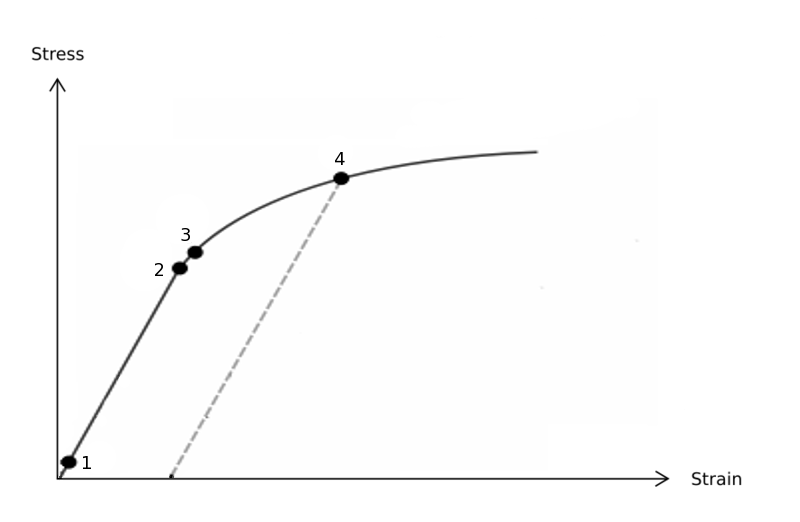
\includegraphics[width=7.5cm]{./images/physics_ssc_metal.png}
    \label{fig:ssc-restshape}
  }
  \subfloat[Stress-strain curve of strain hardening and necking.]{
    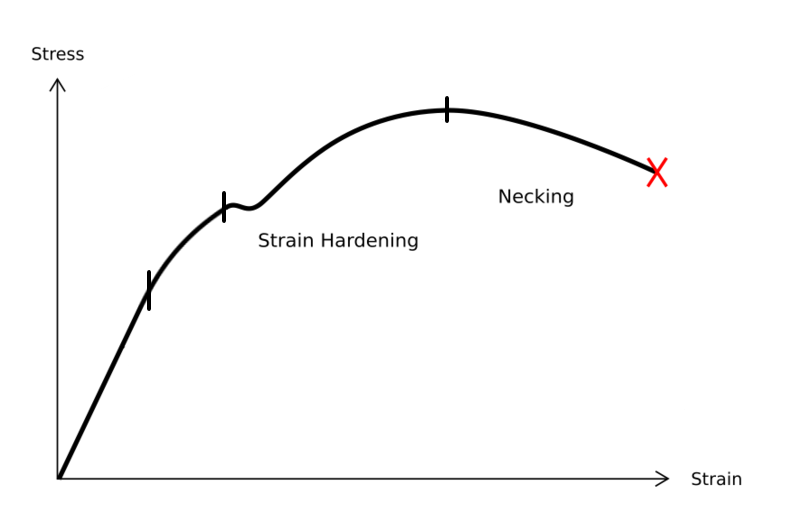
\includegraphics[width=7.5cm]{./images/physics_ssc_necking.png}
    \label{fig:ssc-necking}
  }
  \caption{Stress-strain curves illustrating plastic deformation.}
  \label{fig:ssc-plasticity}
\end{figure}

% \begin{figure}
%   \centering
% \end{figure}

Plastic deformation covers many distinct physical
processes. \defit{Strain hardening} and \defit{necking} are both
examples of physical processes which can be seen on the stress-strain
curve as illustrated in figure \vref{fig:ssc-necking}.
%
%\defit{Strain hardening}
Strain hardening or \defit{work hardening} is when a material becomes
increasingly saturated with dislocations. When more and more
dislocations are introduced the material starts to develop a
resistance against new dislocations. This resistance shows itself as a
strengthening of the material \citebook{page~194}{book:material-science}.
%
%\defit{Necking}
When a material is plastic deformed, and after the material's ultimate
strength limit has been reached \defit{necking} begins. The term
\defit{neck} refers to a point in the material where the material
gets weaker than the rest of the material. Necking is part of
the fracturing process for soft materials like metal
\citebook{page~223}{book:material-science}.

\subsection{Fracture}
If deformation exceeds the point of fracture, the material
collapses hereby releasing its internally stored forces. Material
collapse, known as fracture, is a subject of its own:
\defit{Fracture mechanics}. Fracture mechanics is elaborated in
section \vref{sec:fracture-mechanics}.

% \subsection{Additional Deformation Phenomena}

% \subsubsection{Fatigue}
% When a material is deformed in the elastic range, it completely returns to
% its original shape when forces are removed. But sometimes faults are
% introduced at the level of molecules. After many deformations,
% cracks will begin to appear, followed by fractures. The material will
% fracture with no apparent plastic deformation in between. 
% This phenomenon is known as \defit{fatigue}, and is most
% commonly observed in metals \citebook{page~225}{book:material-science}.

% \subsubsection{Hysteresis}
% Some elastic materials behave in one way when loaded, and another when
% unloaded. This phenomenon
% is know as hysteresis. Figure \vref{fig:ssc-hysteresis} is an example
% of a stress-strain curve for a material with hysteresis.
% %
% If the amount of work it takes to deform an object differs from
% the amount used to reverse the process, the material has
% hysteresis \citebook{page~345}{book:uni-physics}.

% \begin{figure}
%   \centering
%   \includegraphics[width=7.5cm]{./images/ssc-hysteresis.png}
% \caption{Stress-strain curve of hysteresis}
% \label{fig:ssc-hysteresis}
% \end{figure}

\subsection{Brittle and Ductile Materials}
\label{sec:brittle-ductile}
Solid materials can be categorised according to their material
properties. Before reaching the point of fracture, a material will
undergo plastic deformations to some extent.
%
If the amount of plastic deformation in a material is almost
non-existing, as in the case of glass, it is reasonable to neglect
this type of deformation. When this is the case the material is
considered \defit{brittle} and the point of yield strength $\approx$
fracture point.
%
Materials, like metal, where plastic deformation is important are
known as \defit{ductile} materials \citebook{page~345}{book:uni-physics}.
%
% Fatigue primarily occurs in ductile materials. Figure
% \vref{fig:ssc-brittle-and-ductile} illustrates stress-strain curves for
% typical brittle and a ductile materials.

% \begin{figure}
%   \centering
%   \subfloat[Brittle]{
%     \includegraphics[width=7cm]{./images/ssc-brittle.png}
%     \label{fig:ssc-brittle}
%   }
%   \subfloat[Ductile]{
%     \includegraphics[width=7cm]{./images/ssc-metal.png}
%     \label{fig:ssc-ductile}
%   }
%   \caption{Stress-strain curves for brittle and ductile materials}
%   \label{fig:ssc-brittle-and-ductile}
% \end{figure}


\subsection{Variations in the Material Properties}
Materials can have different properties when compressed compared
to when stretched. Concrete for example, is much stronger
when compressed than when stretched. Figure
\vref{fig:ssc-stretch-and-compression-fragture} illustrates this in one
stress-strain curve by using that compressive strain is negative. Here
the fracture point is much higher under compression that under
stretch.
%
The material can have a particular stress and strain relation under compression
and another when stretched, hereby yielding two different slopes, as
illustrated in figure \vref{fig:ssc-stretch-and-compression-moduli}.
% When this is the case we
%denote the elastic moduli $E_+$ and $E_-$. \\
%

\begin{figure}
  \centering
  \subfloat[Different fracture points.]{
    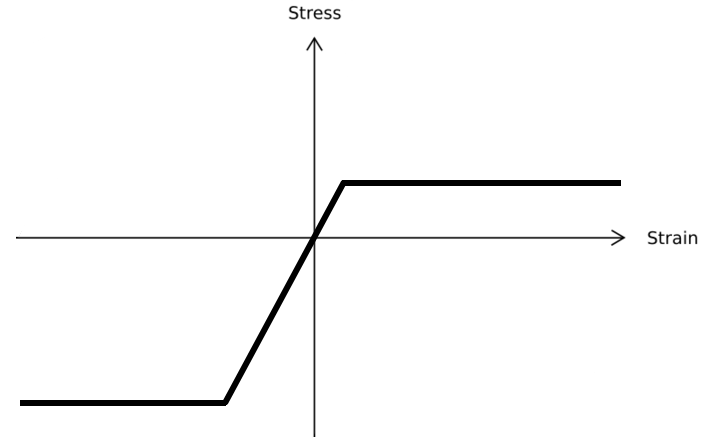
\includegraphics[width=7.5cm]{./images/physics_ssc_stretch_compression_fragture.png}
    \label{fig:ssc-stretch-and-compression-fragture}
  }
  \subfloat[Different slope.]{
    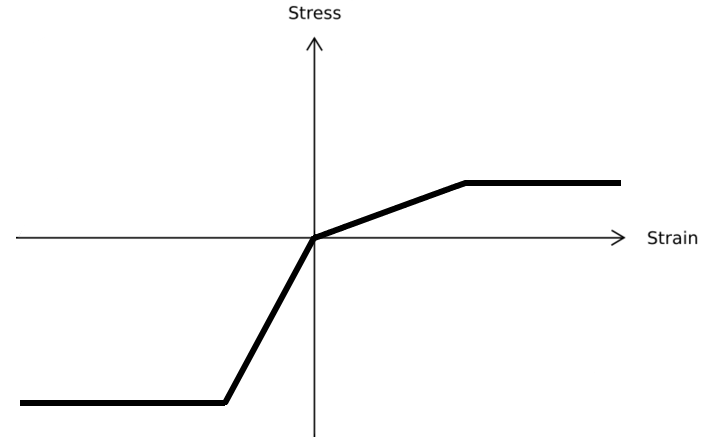
\includegraphics[width=7.5cm]{./images/physics_ssc_stretch_compression.png}
    \label{fig:ssc-stretch-and-compression-moduli}
  }
  \caption{Stress-strain curves of materials with different properties during compression contra stretch.}
  \label{fig:ssc-stretch-and-compression}
\end{figure}

% Material properties depend on many other parameters of the
% surroundings, like temperature, pressure and humidity.
% When modeling a material the influence of such phenomena most be
% taken into account individually.

% - Elasticity
% - - Material properties
\section{Linear Elasticity}
\label{sec:elasticity}
% material science, p. 181
% Because we want to model brittle material, only the elastic
% deformation of a material is of interest. Elastic deformation can
% either be linear, non-linear or both and the elastic properties depend
% on the material as described in section \vref{sec:elastic-deformation}.
% %
% In the following section we will introduce the linear elasticity
% theory for isotropic materials. 
% An \defit{isotropic material} is a material that has the same
% properties in all directions. 
%
When modeling brittle material, only the elastic
deformation of a material is of interest, and we shall assume that the
stress-strain relation is linear. Furthermore we shall assume that the
material is \defit{isotropic}, i.e. that it has the same properties is
all directions.
%
Linear elasticity in the simplest form is described by 
\defit{Hooke's law} of elasticity. Hooke's law relates deformation and
external forces by stating: \defit{Extension of a
material is in direct proportion with the forces acting upon it}. This is
true as long as the force does not exceed the elastic proportional
limit. The most commonly encountered form of Hooke's law is \defit{the
  spring equation}, which relates the force exerted by a spring to the
distance it is stretched or compressed by a spring constant $k$
measured in force per unit length ($N/m$). 

\begin{equation}
\label{eq:hooks_law}
    f = -k \cdot \Delta x
\end{equation}

The negative sign indicates that the force exerted by the spring is in
opposite direction of the displacement.
%
To extend Hooke's Law into three dimensions we need to introduce more
than one constant which relates forces and deformation. In keeping
with generally used terms in theory of linear elasticity these
constants are denoted moduli.
%
%Like the spring constant, a modulus relates forces to deformation hence
%stress to strain. A modulus relates stress and strain as follows:
%$\frac{stress}{strain}$.
%
More than one modulus enables us to relate the degrees of freedom in
three dimensions. There are many different moduli or constants in linear
elasticity but we only need two: the elastic modulus and Poisson's ratio,
and how they relate stress and strain to cover all degrees of freedom.

\subsection{Modulus of Elasticity}
The \defit{elastic modulus} or \defit{Young's modulus} $E$ relates normal
strain and normal stress and is defined to be:

\begin{equation}
\label{eq:normal_stress_over_normal_strain}
  E =  \frac{\mbox{normal stress}}{\mbox{normal strain}}
  = \frac{\sigma}{\varepsilon}
  \qquad \Leftrightarrow \qquad
  \varepsilon = \frac{\sigma}{E}
\end{equation}

The elastic modulus is
material dependent and can be found in reference books like
\citeabook{book:springer-materials}. Seen on a stress-strain curve a 
modulus is the slope of the linear piece of the graph. A high modulus 
indicates a hard or stiff material whereas a low modulus indicates a
soft elastic material.
%A relationship between $E$ and $G$ exists, this
%relationship includes elastic constant, referred to as Poisson's
%ratio. Poisson's ratio must be introduced before the relationship can
%be explained.

% below copied from tled report, spg tic om det er ham der har
% skrevet det
\subsection{Poisson's Ratio}
\label{sec:poissons_ratio}
When a body is stretched or compressed in one direction, it tends to
contract or expand in the opposite two directions. Poisson's ratio
$\nu$ is a direct measurement of this phenomenon for isotropic
materials. Consider a material in two dimensions, when it is
compressed by a force along the $x$-axis it results in the strain
$\varepsilon_x$. Due to the compression the material will expand 
$\varepsilon_y$ in the y direction, as follows:

\begin{equation}
  \varepsilon_y = - \nu \varepsilon_x
    \qquad \Leftrightarrow \qquad
    \nu =
    -\frac{\varepsilon_x}{\varepsilon_y} =
    -\frac{\Delta x / x}{\Delta y / y}
\end{equation}

Here $\nu$ is Poisson's ratio, relating the compression and
expansion. To express this as stress, we use equation
\eqref{eq:normal_stress_over_normal_strain} and get:

\begin{equation}
  \varepsilon_y = - \nu \varepsilon_x = - \nu \frac{\sigma_x}{E}
\end{equation}

Like the elastic modulus, Poisson's ratio can be found in reference
books.

\subsection{Relating Stress and Strain in Three Dimensions}
\label{sec:stress-strain-relation-in-3d}
To relate stress and strain in three dimensions, we need to combine
the elastic modulus and Poisson's ratio in all dimensions.
%
%If stress other than pure tensile or pure shearing is applied, the
%material behaviour gets a bit more complicated. 
%
Consider a cubic element with normal stress $\sigma_x$, $\sigma_y$
and $\sigma_z$ acting in the $x$, $y$, and $z$ direction, respectively.
%
% According to equation 
% \eqref{eq:normal_stress_over_normal_strain} the cube will stretch in the
% x direction by a strain $\varepsilon_x = \sigma_x / E$, and contract
% by a tensile strain of $-\nu \sigma_x / E\ $ in
% the other two directions due to the effect described by Poisson's ratio. 
% Similarly the reaction to tensile stress $\sigma_y$ in the y
% direction will be a tensile strain of $-\nu \sigma_y / E\ $ in
% the x and z direction. 
% % If a stress is applied which is not purely tensile or purely shear
% % then the behavior of the material is more complicated. When a object is
% % subjected to external forces then, as a direct
% % conseqiense of posion's ratio, if one direction is stretched, then
% % others will compress. 
% When modeling isotropic materials, this
% relationship will be uniformly distributed between the other directions
% \citebook{page~185-187}{book:material-science}. \\
% %
%
% From Hooke's Law and Poisson's ratio we obtain an expression of
% tensile strain in each direction:
%
% %It is possible to generalize Hooke's Law into three dimensions
% %via Poisson's ratio, and make all directions dependent:
%
Due to the stress component, $\sigma_x$, the cube will stretch (if
$\sigma_x > 0$) in the $x$ direction by the amount which according to
equation \eqref{eq:normal_stress_over_normal_strain} is $\varepsilon_x
= \sigma_x / E$ and contract in the $y$- and $z$-direction by an amount of
$-\nu \sigma_x /E$. Similarly for the remaining two stress
components. The total deformation of the cube is now found by adding
the various contributions \citebook{page~187}{book:material-science}:

\begin{equation}
\label{eq:hookes-law-in-3d}
\begin{aligned}
    \varepsilon_x &= \frac {1}{E} \left [ \sigma_x - \nu \left (
        \sigma_y + \sigma_z \right ) \right ] \\
    \varepsilon_y &= \frac {1}{E} \left [ \sigma_y - \nu \left (
        \sigma_x + \sigma_z \right ) \right ] \\
    \varepsilon_z &= \frac {1}{E} \left [ \sigma_z - \nu \left (
        \sigma_x + \sigma_y \right ) \right ]  
\end{aligned}
\end{equation}

In equation \eqref{eq:hookes-law-in-3d} the relation between normal
stress and strain are completely defined by the two constants $E$ and
$\nu$. These constants can also be used to relate shearing stress and
strain.
%
%Note that this only accounts for stress and strain in the normal
%directions. As we also model shearing stress and strain, these
%quantities most also be taken into account.
%
The relationship between shearing stress and shearing strain is 
called the \defit{Shear modulus} or \defit{modulus of rigidity} and is
denoted $G$.

\begin{equation}
\label{eq:shearing_stress_over_shearing_strain}
  G 
  %= \mu
  = \frac{\mbox{shear stress}}{\mbox{shear strain}}
  = \frac{\tau_{xy}}{\gamma_{xy}}
  \qquad \Leftrightarrow \qquad
  \gamma_{xy} = \frac{\tau_{xy}}{G}
\end{equation}

The shear modulus can be deduced from $E$ and $\nu$ as done in
\citebook{page~9-10}{book:theory-of-elasticity}, the relation is:

\begin{equation}
\label{eq:EG-relation}
  G = \frac{E}{2(\nu+1)}
\end{equation}

Shearing in one direction does not affect shear in other
directions. Note that shear is independent of normal stress and
strain \citebook{page~266}{book:deformable-solids}. For shear in three
dimensions, the equations are defined as:

\begin{equation}
\label{eq:3d-shear-ss-relation}
  \gamma_{xy} = \tau_{xy} / G
  \qquad
  \gamma_{yz} = \tau_{yz} / G
  \qquad
  \gamma_{zx} = \tau_{zx} / G
\end{equation}


% Fracture Mechanics
\section{Fracture Mechanics}
\label{sec:fracture-mechanics}
\defit{Fracture mechanics} describes what happens to a material when
the fracture point limit has been exceeded.
%
When the material reaches this limit, a fracture is initiated at a
specific \defit{crack point} within the material. The fracture
propagates by opening a crack inside the material along a
\defit{fracture plane}. The crack can be described by connected
\defit{crack surfaces}. The crack opens to release
potential energy accumulated within the material. The internal potential
strain energy, is used to create
new \defit{crack surfaces} by ripping part of the body into surfaces.
This conversion of body to surface requires work, which is
how the energy is released \citebook{page~218}{book:material-science}.
%
The \defit{crack length} is determined by the amount of internally
stored energy contra how much energy it takes to create the new surfaces.
%
When considering an isotopic material in three dimensions, we idealize
the crack surfaces by using two surfaces, which form a lens as
illustrated in figure \vref{fig:crack-surfaces}.

% \begin{figure}
%   \centering
%   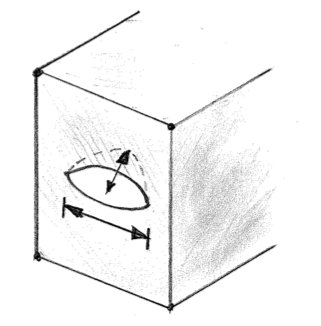
\includegraphics[width=6cm]{./images/physics_crack_surfaces_0.png}
%   \caption{Crack surfaces.}
%   \label{fig:crack-surfaces}
% \End{figure}

\begin{figure}
  \begin{minipage}[b]{0.5\linewidth}
    \centering
    \subfloat[Half lens.]{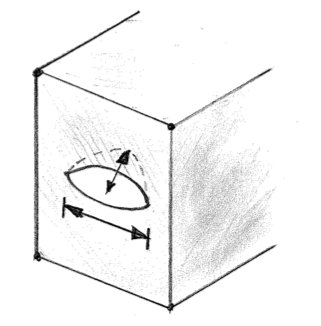
\includegraphics[width=70mm]{./images/physics_crack_surfaces_0.png}}
  \end{minipage}
  \hspace{0.5cm}
  \begin{minipage}[b]{0.5\linewidth}
    \centering
    \subfloat[Quarter of a lens.]{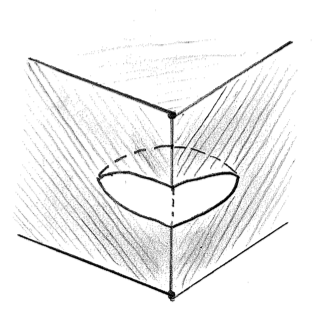
\includegraphics[width=70mm]{./images/physics_crack_surfaces_1.png}}
  \end{minipage}
  \caption{Two crack surfaces forming a lens.}
  \label{fig:crack-surfaces}
\end{figure}

%The analytical formulas for calculating the strain energy along the
%crack in three dimensions are very complex and beyond the scope of 
%will be omitted, but
%We will return to the subject of fracture mechanics when constructing
%a discrete model in section \vref{sec:discrete-fracture-mechanics}.

% crack initial via max pr stress.
\subsection{Crack Initialization}
\label{sec:physics_crack_init}
% include that there are teories for having more than one crack init.
There are different theories of how to calculate the crack
initialization point. We use: \defit{maximum principal stress} since this
technique has proved suitable for brittle materials
\citebook{page~370}{book:strength-materials}.
%
\defit{Principal stress} is a measure where both shearing and normal
stress is incorporated, yielding three vectors. The longest vector of
the three reveals in which direction the maximum stress points in a
given point within the material. The method of maximum principal finds
the maximum principal stress of all points in the material, yielding
the precise point and direction of the stress.
%
If this stress exceeds the fracture point ($\sigma_F$), the material
breaks in this precise location. If a material has different
fracture point limits when stretched or compressed, they are
denoted: $\sigma_F^+$ and $\sigma_F^-$.
% 
How to calculate the principal stress based on normal and shearing
stress will be elaborated in section
\vref{sec:principal_values_and_directions}, when linear transformation
has been introduced.
%
The principal stress also contains information about how the crack
surfaces will form. The vector direction defines the normal of the
crack plane.

\subsection{Crack length}
The energy it takes to form the new surface is determined by the
crack surfaces area and the \defit{strain energy release rate}, which
is a material property.
The length of the crack is determined by the amount of strain energy
stored in the point where the crack opens and the amount it takes to
create the crack surfaces. The amount of energy used to create a
surface in a given material depends upon the material itself and on
the area of the crack surfaces. The area of the surfaces when using
the lens form is further approximated by using a circle. This is done
because the lens is much wider that thick and therefore a circle
covers most of the area as illustrated in figure
\vref{fig:crack-surfaces-from-above}, where the crack is seen from
above. The circle area is calculated by: $A = \pi a^2$.

% \begin{figure}
%   \centering
%   \includegraphics[width=6cm]{./images/material-science-p218-f9-31.png}
%   \caption{Crack surfaces seen from above}
%   \label{fig:crack-surfaces-from-above}
% \end{figure}

\begin{figure}
  \centering
  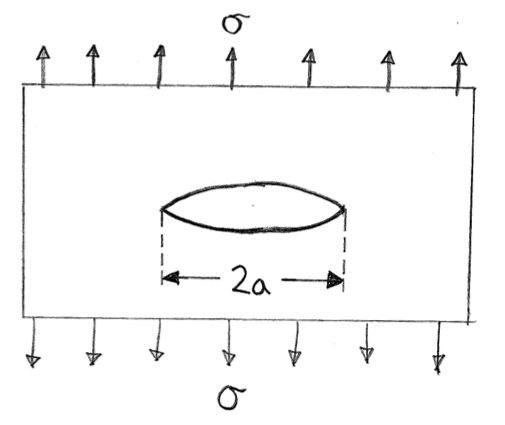
\includegraphics[width=7cm]{./images/physics_crack_surfaces_from_above.png}
  \caption{Crack surfaces seen from above.}
  \label{fig:crack-surfaces-from-above}
\end{figure}


%And can be use to calculate the stress at the \defit{crack tip}. The
%stress $\sigma_{tip}$ for an elliptical section is given by
%\citebook{page~218}{book:material-science}:

%\begin{equation}
%\sigma_{tip} = 2 \sigma \left( \frac{a}{\rho} \right)^{1/2}
%\end{equation}

%Where $\rho$ is the radius for the \defit{dominant zone}. The dominant
%zone ...

% *** insert figure from: applied solid mechanics, section 9.3.2


%The strain energy is calculated as:
%\begin{equation}
%  E_E = \int_V \sigma \cdot \varepsilon
%\end{equation}

%But for at crack of unit width, can be approximated by:
%\begin{equation}
%  E_E = \sigma \varepsilon V
%  = \frac{\sigma^2 V}{E}
%  = \frac{\sigma^2 \pi a^2}{E}
%\end{equation}

%\begin{equation}
%  U_S = = 2 G_C a = 4 \gamma a
%\end{equation}

%We use the energy relation from  \vref{sec:energy-} to relate the 

%\begin{equation}
%  U = U_E + U_S = 0 \Leftrightarrow - U_E = U_s
%\end{equation}

%Energy release:

The crack continues to grow until the strain energy cannot expand 
the crack surfaces further. Figure \vref{fig:energy-release-graph}
illustrates an example of this.
%
The graph $E_C$ depicts the amount of energy it takes to produce the
crack surfaces as a function of the crack length $a$. 
%
%This means that larger crack surfaces requires more energy to produce.
%
The graph $E_S$ is the internal strain energy in the body.
%
Focusing on graph $E_T$ this graph describes the total
energy ($E_T = E_C + E_S$), here the fracture point is reached
at the dotted line, and a crack is initialized, hereby releasing
energy.
%
Looking at the strain energy function $E_S$ we see that this energy
rapidly increases as the crack starts to propagate.
%
When the $E_T$ graph crosses the $x$ axis, there is no more energy
left and the crack propagation stops.

\begin{figure}
  \centering
  \subfloat[Strain contra surface energy.]{
   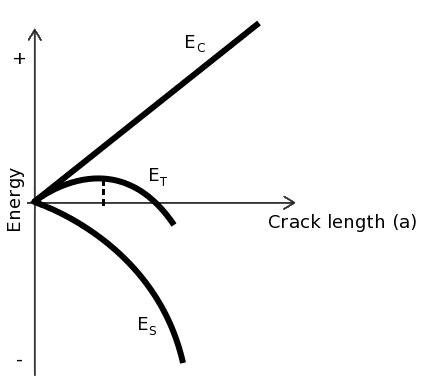
\includegraphics[width=6cm]{./images/physics_energy_release_graph.png}
   \label{fig:energy-release-graph}
  }
  \qquad
  \subfloat[Derivatives of strain and surface energy.]{
   \includegraphics[width=6cm]{./images/physics_energy_graph.png}
   \label{fig:energy-graph}
  }
  \caption{Strain contra surface creation energy.}
  \label{fig:energy-graphs}
\end{figure}

Figure \vref{fig:energy-graph} illustrates the energy derivatives of
$E_C$ and $E_S$ from figure \vref{fig:energy-release-graph}. Here the
point where the strain energy exceeds the surface creation energy
becomes directly apparent \citebook{page~219-221}{book:material-science}.
%
In figure \vref{fig:energy-graph}, the following notation is used:

\begin{equation*}
dS = \frac{\partial E_S}{\partial a} \qquad \qquad dC = \frac{\partial E_C}{\partial a}
\end{equation*}



% open via energy, 
%\subsection{Energy}

% below copied from wiki:
% http://en.wikipedia.org/wiki/Strain_energy_release_rate
%Strain energy release rate (or energy release rate) is the energy
%dissipated during fracture per unit of newly created fracture surface
%area
% above copied from wiki: 
% http://en.wikipedia.org/wiki/Strain_energy_release_rate

\subsection{Crack propagation}
%For the crack to reach the materials outer surfaces, the crack must
%propagate all the way to this surface. 
%
% korteste vej til overfladen.
%The crack always steers towards the outer surface, hereby releasing
%the maximum amount of energy possible \citebook{}{}.
%
% ref som siger at hvis der allerede er en crack, forsættes denne.
%
Brittle material often has a single crack propagating through the
entire material \citebook{section~9.1}{book:solid-mechanics}.
%
% hastighed: lydens.
Once the crack begin to propagate, the stress required for further
propagation decreases as $a$ increases and therefore the crack
accelerates rapidly \citebook{page~220}{book:material-science}.

% note på at det med vinkler er realistisk for hårde materialer.



% energi ophobes
% når energien når over det niveau hvor sigma_max difinere arealet A
% laves de nye surfaces, og alt energien frigives.




% \subsection{Generalized stress modes}
% When the crack propagated it can be stressed by deformation
% of the body.
% This kind of stress is generalized into three different modes. Normal
% stress ... to \defit{opening mode} or \defit{mode I}, where the crack
% surfaces are perpendicular to the crack plane. In plane-shear result in \defit{sliding mode} or
% \defit{mode II}, here the displacement of the crack surfaces is in the
% plane of the crack and perpendicular to the crack front. The last,
% \defit{mode III} or \defit{tearing mode} is caused by out of plane
% shear \citebook{page~9}{book:elementary-fm}. The three modes are
% illustrated in figure \vref{}. Often more than one mode is
% pressent at the same time, when this happens we call it \defit{mixed
%   mode}.

% \begin{figure}
%   \centering
%   \includegraphics[width=5cm]{./images/elementary-fm-p25-f2-1.png}
%   \caption{The three modes of stress in the crack front}
%   \label{fig:stress-in-crack-front}
% \end{figure}


\chapter{Mathematics}
\label{chapter:mathematics}
% -*- mode: latex; mode: auto-fill; coding: utf-8; -*-

\section{Linear Transformations}
\label{sec:linear_transformation}
A linear transformation, or linear mapping, is a function $f$ that maps
one vector space into another with the property that \citebook{page~175}{book:leon}:

\begin{equation}
f(\alpha x + \beta y) = \alpha f(x) + \beta f(y)
\end{equation}

where $\alpha$ and $\beta$ are scalars.
An \defit{affine} transformation from a Euclidean space into another is
a mapping which preserves collinearity of points and ratios of
distances between points on a straight line. In other words, points which lie
on a straight line before the transformation continue to do so after the transformation is
applied. Consider point $a$, $b$ and $c$, the ratio $\frac{ \vert
  b-a\vert}{\vert c-b \vert}$ is preserved when using affine transformations.
An affine transformation can be a translation, a rotation, a scaling,
a shear or a combination hereof using matrix
multiplication \citebook{page~2}{book:3d-games}.
%
A common form of a linear equation in two variables, $x$ and $y$ is 

\begin{equation}
\label{eq:linear-equation}
y = A x + b
\end{equation}

where $A$ is a matrix representing rotation, scaling or shearing and
$b$ represents translation. 
The set of solutions to this equation forms a straight line hence the
name linear. Using \defit{homogeneous} coordinates means representing an
$n$-dimensional vector by $(n+1)$ components. This way we can
include translation in the set of affine transformations and hereby get rid of
$b$ in equation \eqref{eq:linear-equation}. 
The following examples show commonly used affine transformations. \\

\subsection*{Translation}
\label{sec:basic_math_translation}
Here is an example of an affine three-dimensional translation:
\begin{equation}
\label{eq:translation_matrix}
T = 
\begin{bmatrix} 
1 & 0 & 0 & t_x \\ 
0 & 1 & 0 & t_y \\ 
0 & 0 & 1 & t_z \\
0 & 0 & 0 & 1 
\end{bmatrix} 
\end{equation} 

$t_x$, $t_y$ and $t_z$ are the axial translations in the $x$, $y$, and $z$
axis respectively. Only the rightmost column concerns the
translation as opposed to scaling, rotation and shearing where only
the upper-left $3\times3$ sub-matrix defines the transformation.
Any affine transformation matrix can be applied to a vector $4 \times
1$ vector $v$ by using matrix multiplication $v^\prime = T \ v$:

\begin{equation}
%\label{eq:translation_matrix}
\begin{bmatrix} 
x' \\ y' \\ z' \\ 1 
\end{bmatrix} 
= 
\begin{bmatrix} 
1 & 0 & 0 & t_x \\ 
0 & 1 & 0 & t_y \\ 
0 & 0 & 1 & t_z \\
0 & 0 & 0 & 1 
\end{bmatrix} 
\begin{bmatrix} 
x \\ y \\ z \\ 1 
\end{bmatrix}
\end{equation} 

Notice that the fourth vector component has the value one since it is
in homogeneous form. This way translation can be applied using
matrix multiplication instead of the standard vector addition as shown
in equation \eqref{eq:linear-equation}. \\ 

\subsection*{Scaling}
\label{sec:basic_math_scaling}
This is an affine scaling matrix:
%Here is an example of an affine scaling:
\begin{equation}
\label{eq:scaling_matrix}
S = 
\begin{bmatrix} 
S_x & 0 & 0 & 0 \\ 
0 & S_y & 0 & 0 \\ 
0 & 0 & S_z & 0 \\
0 & 0 & 0 & 1 
\end{bmatrix} 
\end{equation} 

$S_x$, $S_y$, and $S_z$ are the scaling factors in the $x$, $y$, and $z$
axis respectively. \\

\subsection*{Shearing}
\label{sec:basic_math_shearing}
Generally shearing can be performed
in an arbitrary plane. There are six basic shearing matrices
\citebook{page~31}{book:realtime}. One for each 
off-diagonal component in the upper-left $3\times3$ matrix as
illustrated here:
 
\begin{equation}
\label{eq:shearing_matrix}
H = 
\begin{bmatrix} 
1 & S_{xy} & S_{xz} & 0 \\ 
S_{yx} & 1 & S_{yz} & 0 \\ 
S_{zx} & S_{zy} & 1 & 0\\
0 & 0 & 0 & 1 
\end{bmatrix} 
\end{equation} 

For simplicity the following example only illustrates
shearing acting in planes orthogonal to axis of the coordinate
frame. The following is an example of a shearing matrix in the
$xy$-plane: 

\begin{equation}
\label{eq:shearing_matrix_xy_plane}
H_{xy} = 
\begin{bmatrix} 
1 & t & 0 & 0 \\ 
0 & 1 & 0 & 0 \\ 
0 & 0 & 1 & 0\\
0 & 0 & 0 & 1 
\end{bmatrix} 
\end{equation} 

The result of applying the $H_{xy}$ shearing matrix to a unit square is
illustrated in figure \vref{fig:mathematics_unit_square_shearing}.


%% Figure showing shearing of unit square.
\begin{figure}
  \centering
  \subfloat[Before]{
    \includegraphics[width=6cm]{./images/mathematics_shearing_unit_square_before.png}
  }
  \subfloat[After]{
    \includegraphics[width=6cm]{./images/mathematics_shearing_unit_square_after.png}
  }
\caption{Shearing in the xy-plane applied to a unit square.}
\label{fig:mathematics_unit_square_shearing}
\end{figure}

\subsection*{Rotation}
\label{sec:basic_math_rotation}
Generally rotation can be applied around an arbitrary axis but for
simplicity the examples here are limited to rotations around the $x$, $y$, and $z$ axis.
The following three examples illustrate counter-clockwise rotation $\theta$ degrees
around the $x$, $y$, and $z$ axis respectively:
\begin{equation}
\label{eq:rotation_matrix_x}
R_x = 
\begin{bmatrix} 
1 & 0 & 0 & 0 \\ 
0 & cos \theta & - sin \theta & 0 \\ 
0 & sin \theta & cos \theta & 0\\
0 & 0 & 0 & 1 
\end{bmatrix} 
\end{equation} 
\begin{equation}
\label{eq:rotation_matrix_y}
R_y = 
\begin{bmatrix} 
cos \theta & 0 & sin \theta & 0 \\ 
0 &  1 & 0 & 0 \\ 
- sin \theta & 0 & cos \theta & 0\\
0 & 0 & 0 & 1 
\end{bmatrix} 
\end{equation} 
\begin{equation}
\label{eq:rotation_matrix_z}
R_z = 
\begin{bmatrix} 
cos \theta & - sin \theta & 0 & 0 \\ 
sin \theta & cos \theta & 0 & 0 \\ 
0 & 0 & 1 & 0\\
0 & 0 & 0 & 1 
\end{bmatrix} 
\end{equation} 

Constructing an affine rotation matrix requires certain matrix
properties. To ensure preservation of collinearity and ratio of
distances between points along lines the rotation matrix must be an
\defit{orthogonal} matrix. An
orthogonal rotation matrix is by definition a square matrix with rows
(or columns) that
form an \defit{orthonormal basis} \citebook{page~258}{book:leon}. An orthonormal
basis is a set of mutually perpendicular vectors all of magnitude
one \citebook{page~255}{book:leon} as illustrated in figure
\vref{fig:orthonormal_basis}.  

\begin{figure}
  \centering
  \includegraphics[width=6cm]{./images/mathematics_orthogonal_matrix.png}
\caption{An orthonormal basis.}
\label{fig:orthonormal_basis}
\end{figure}
  
The determinant of any orthogonal matrix is either $+1$ or $-1$. If the
determinant equals $-1$ it forms a reflection matrix rather than a
rotation matrix.
If the determinant of the orthogonal matrix equals $1$ it forms a
rotation matrix and these are the ones we are interested in. 
%
A rotation matrix has the following useful properties:

\begin{itemize}
\item Columns (or rows) are orthogonal unit vectors.
\item The transpose equals the inverse:
\begin{equation}
\label{eq:inverse_equals_transposed}
A A^T = A^T A = A^{-1} A = I
\end{equation}
\item The determinant equals $+1$.
\item Closed under multiplication and the inverse operation. 
\end{itemize}

The fact that the inverse
of a rotation matrix is the same as the transpose is very
useful. The transpose of a matrix can be found just by swapping rows
with columns, whereas finding the inverse usually means solving a system of
linear equations using Gaussian elimination or another solving
technique, so generally transposing a matrix is computationally much
faster. 


\section{Tensors}
\label{sec:tensors}
Tensors are a powerful abstraction proven
very useful especially in physics and engineering. Because of its
abstractness it is not an easy entity to describe. A tensor is a way
of describing linear transformations according to certain rules.
A tensor is in fact just a linear function, but in applied
mathematics it sometimes seems like a ``magic'' entity. \\  


% TENSOR EXAMPLE 
% sailor http://en.wikibooks.org/wiki/General_relativity:What_is_a_tensor%3F
%The use of tensors are probably best explained though examples.

The use of tensors is probably best motivated through an
example. Consider the life of a pirate sailing on the ocean only
powered by the wind.
Dependent on the weather conditions the wind
will have a certain speed and come from a certain direction. Wind could easily
be represented as a vector $v$ where the magnitude of the vector
represents the wind speed. When the wind hits the sail it produces a
force that will make the ship move. If the ship was always sailing in the
same direction as the wind we could just represent the relation between
wind and force with a simple scalar. The resulting
force vector could simply be obtained by multiplying the wind vector with the
scalar. You don't have to be a sailor to see that if the ship
could only move in the direction of the wind only random sailing would
be possible. Sailing is more complicated in real life. We need to
represent the relation between wind and resulting force in a different
way. We shall assume that this relation is linear, so doubling the
wind speed will double the force. We could represent this linear relation
between the wind and the force on matrix form:

\begin{equation}
T = 
\begin{bmatrix} 
\tau_{11} & \tau_{12} \\
\tau_{21} & \tau_{22} \\
\end{bmatrix} 
\end{equation}

Here $T$ is an example of a tensor capable of relating two different quantities,
one is the wind speed and direction the other is the force direction
and magnitude. The resulting force could be expressed as:

\begin{equation}
f = T \cdot w
\end{equation}

where $T$ is the tensor, $w$ and $f$ is the wind and
force vector, respectively.

\begin{figure}
  \centering
  \includegraphics[width=10cm]{./images/mathematics_tensor_pirate_ship.png}
\caption{Wind from behind hits the sail and produces force.}
\label{fig:tensor_pirate_ship}
\end{figure}

As illustrated on figure \vref{fig:tensor_pirate_ship} the pirate ship with its sail set, is
going in a direction say $45^\circ$ to the right of the wind
direction. We represent the wind direction and speed as $w =
[1,1]^T$ hereby setting the wind speed to the length of the vector
which equals $\sqrt{2}$. Let's say each wind speed unit produces two force 
units. A tensor representing this linear relation in direction and
magnitude can be written in matrix form:

\begin{equation}
T = \begin{bmatrix} 
2 \cdot (\cos \theta) & 2 \cdot (-\sin \theta) \\ 
2 \cdot (\sin \theta) & 2 \cdot (\cos \theta) 
\end{bmatrix} 
\end{equation}

where $\theta$ defines the angle the vector will be rotated.
The force produced by the wind can be obtained by:

\begin{equation}
f = 
\begin{bmatrix} 
2 \cdot (\cos 45) & 2 \cdot (-\sin 45) \\ 
2 \cdot (\sin 45) & 2 \cdot (\cos 45) 
\end{bmatrix} 
\begin{bmatrix} 
1 \\ 1
\end{bmatrix} 
=
\begin{bmatrix}
0 \\ 2.828 
\end{bmatrix} 
\end{equation}

Using tensor algebra we can begin to see why these abstract tensor
entities are powerful. In the example we did only have one linear
relation between wind and force, so we did only represent a single sail. A pirate ship
probably has many sails with different size hence different linear
relations between wind and force. The total force when three sails are
set is obtained by:

\begin{equation}
\label{eq:tensor_concat}
f = R \cdot w + S \cdot w + T \cdot w
\end{equation}

where $w$ is the wind and $R$, $S$, and $T$ are the three tensors each representing a linear
relation between wind and force produced.
Since wind with its direction and speed is constant equation
\eqref{eq:tensor_concat} can be written as:

\begin{equation}
f = (R + S + T) \cdot w
\end{equation}

Due to the fact that $R$, $S$, and $T$ are on matrix form and are
linear they can be combined to form a new tensor $U$:

\begin{equation}
U = R + S + T
\end{equation}  
\begin{equation}
f = U \cdot w
\end{equation} \\

Tensors are all about linear relations. Tensors of different orders
exist and we will classify tensors according to
their order. All tensors can be represented by $n$-dimensional
arrays where $n$ equals the tensor order. The number of indices needed to 
address each individual element in a tensor corresponds to the order. A
scalar needs zero indices, a vector needs one, a matrix needs two
etc. \\

A \defit{zero order} tensor is simply a scalar and can be represented by a
zero dimensional array e.g. just a single value. This scalar could
represent the mass of a particle or the volume of an object. An
example of a scalar could be the density of some fluid as a
function of the position. \\

A \defit{first order} tensor can be represented as
a vector. Just like tensors a vector may be
defined at a single point, or it may continuously vary from point to
point hereby defining a vector field. Imagine how to model speed and
direction of fluid through space. Each vector in the field has a
direction and magnitude representing movement and speed
respectively. In three dimensions a vector has three components, in
four dimensions it has four, in n-dimensional space it has n
components still representable as a first order tensor. \\

A \defit{second order} tensor can be represented by a two-dimensional array,
written out as a matrix. In three dimensions a second order tensor
can be represented by a $3 \times 3$ matrix defining e.g. body stretch and
rotation. If multiplying a vector by a second order tensor, the result
is another vector by definition, so a second order tensor is a linear mapping of a
vector onto another vector as in the example with the pirate
ship. Second order tensors are very useful for describing movement and
deformation of volumetric models. In continuum mechanics stress and
strain are often best represented by second order tensors. \\ 

Tensors of all orders can be defined but
as the order of the tensor increases so does the complexity. We will
limit our discussion to second order tensors in three-dimensional
space. \\


Before introducing an actual tensor definition it would be appropriate to
introduce some basic terminology. Throughout the discussion second order tensors will be
represented in the Cartesian coordinate frame spanned by orthonormal
vectors $e_i$, where $i \ \epsilon \ \lbrace 1,2,3 \rbrace$. A vector 
$u$ in this frame is given by 

% Def. bathe 2.48 page 40
\begin{equation}
\label{eq:bathe_2_48}
u = \sum^3_{i=1} u_i e_i
\end{equation}

Vector $u$ represented in the Cartesian coordinate frame is
illustrated in figure \vref{fig:unprimed_coordinate_frame}. 
% Figure of standard coordinate frame with vector v
\begin{figure}
  \centering
  \includegraphics[width=6cm]{./images/mathematics_unprimed_cf.png}
\caption{Vector $u$ in coordinate frame spanned by $e_i$, where $i \ \epsilon \ \lbrace 1,2,3 \rbrace$.}
\label{fig:unprimed_coordinate_frame}
\end{figure}

% Einstein convention
In vector and especially tensor literature a special index
notation if often used. If an index is repeated in a product of
vectors or tensors, summation is implied over the repeated index. This
is also known as the \defit{Einstein Convention} and means the following
is equivalent

\begin{equation}
\delta = a_ib_i \ \ \equiv \ \ \delta = \sum^3_{i=1} a_ib_i \ \
\equiv \ \ \delta = a_1b_1 + a_2b_2 + a_3b_3 
\end{equation} \\

\begin{definition}
\label{def:tensor}
An entity is called a second-order tensor if
it has nine components $T_{ij}$, $i \ \epsilon \ \lbrace 1,2,3
\rbrace$, and $j \ \epsilon \ \lbrace 1,2,3 \rbrace$, in the 
unprimed frame and nine components $T^\prime_{ij}$ in the primed frame and
if these components are related by the characteristic law, defined by:
\begin {equation}
\label{eq:bathe_2_60}
T^\prime_{ij} = P_{il} P_{jm} T_{lm}
\end {equation}
 
\end{definition}

A tensor is defined as an entity,
with components represented in a chosen coordinate frame, that can be
represented in a different coordinate frame, related by the
characteristic law. \\ 

It follows
from definition \vref{def:tensor} that if a tensor equation can be
established in one coordinate frame then it must hold in any other
coordinate frame \citebook{page~502}{book:bathe}. The components of a tensor changes if
the coordinate frame changes. The characteristic law is what 
relates the representation in one coordinate frame to another and it
can also be expressed on matrix form as:

% \begin{equation}
% T^\prime_{mn} e^\prime_m e^\prime_n = T_{kl} e_k e_l
% \end{equation}

% or on matrix from as 

% Def. bathe 2.63 t' = P T P^t
\begin{equation}
\label{eq:primed_stress_tensor}
T^\prime = P \ T \ P^T
\end{equation}

where $P$ is the rotation matrix representing the change of basis from
the primed to the unprimed coordinate frame. The tensor $T$ is  
represented in the unprimed coordinate frame and $P^T$ is the
inverse rotation representing the change of bases from the primed back
to the unprimed coordinate frame. $T^\prime$ is the representation of
the tensor in the primed coordinate frame. \\

Since $P$ is an orthogonal transformation matrix defining a rotation,
the inverse of the transformation equals its transposed matrix
$P^T$ as defined equation \eqref{eq:inverse_equals_transposed}. So a tensor
represented in the unprimed coordinate frame can be obtained by:

% Def. bathe 2.64
\begin{equation}
T = P^T \ T^\prime \ P
\end{equation}

According to definition \vref{def:tensor} any tensor can be
represented in a coordinate frame different from the initial
coordinate frame. 

\begin{figure}
  \centering
  \subfloat[Initial unprimed coordinate frame]{
    \includegraphics[height=6cm]{./images/mathematics_tensor_transform_a.png}
    \label{fig:mathematics_tensor_transform_a}
  }
  \subfloat[Rotated primed coordinate frame]{
    \includegraphics[height=6cm]{./images/mathematics_tensor_transform_b.png}
    \label{fig:mathematics_tensor_transform_b}
  }
  \caption{Transformation of tensor from unprimed to primed coordinate
  frame.}
  \label{fig:tensor_transformation}
\end{figure}


In addition to the unprimed frame, in figure
\vref{fig:mathematics_tensor_transform_a}, consider a primed
coordinate frame. The primed 
coordinate frame spans the same vector space as the unprimed but with
different basis vectors $e^\prime_j$ where $j \ \epsilon \ \lbrace 1,2,3 \rbrace$ as shown in
figure \vref{fig:mathematics_tensor_transform_b}. Now consider any
tensor $T$ represented in the unprimed coordinate frame. The tensor
$T$ can be represented in the primed coordinate frame as
illustrated in figure
\vref{fig:mathematics_tensor_transform_b} through the
relation defined in equation \eqref{eq:primed_stress_tensor},
on matrix form this expands to:

\begin{equation}
  \left[{\begin{matrix} 
        T'_{11} & T'_{12} & T'_{13} \\ 
        T'_{21} & T'_{22} & T'_{23} \\ 
        T'_{31} & T'_{32} & T'_{33} \\ 
      \end{matrix}}\right]
  =
  \left[{\begin{matrix}
        P_{11} & P_{12} & P_{13} \\ 
        P_{21} & P_{22} & P_{23} \\
        P_{31} & P_{32} & P_{33} \\ 
      \end{matrix}}\right]
  \left[{\begin{matrix} 
        T_{11} & T_{12} & T_{13} \\ 
        T_{21} & T_{22} & T_{23} \\ 
        T_{31} & T_{32} & T_{33} \\ 
      \end{matrix}}\right]
  \left[{\begin{matrix} 
        P_{11} & P_{21} & P_{31} \\ 
        P_{12} & P_{22} & P_{32} \\ 
        P_{13} & P_{23} & P_{33} \\ 
      \end{matrix}}\right]
\end{equation}

The diagonal elements of $T'$ represent the scale along the axis of
the primed coordinate frame and the off-diagonal elements represent
shearing.

% In order to discuss this relation in more depth we will
% establish two different coordinate frames and a concrete tensor entity
% to be represented in both.\\

% To establish a second coordinate frame consider, in addition to the unprimed frame in figure
% \vref{fig:unprimed_coordinate_frame}, a primed coordinate frame. The primed
% coordinate frame spans the same vector space as the unprimed but with
% different basis vectors $e^\prime_j$ where $j \ \epsilon \ \lbrace 1,2,3 \rbrace$ as shown in
% figure \vref{fig:unprimed_primed_coordinate_frame}

% % Figure showing primed and unprimed coordinate system
% \begin{figure}
%   \centering
%   \includegraphics[width=6cm]{./images/mathematics_unprimed_primed_cf.png}
% \caption{Different coordinate frames}
% \label{fig:unprimed_primed_coordinate_frame}
% \end{figure}



\subsection{Strain Tensors}
\label{sec:strain_tensors}
As already explained in section \vref{sec:physics_strain} strain
represents the amount of stretch or compression by the relative
distance between two particles in the material body. Strain is a
dimensionless quantity which can be decomposed into normal
strain $\varepsilon$ and
shearing strain $\gamma$. Normal and shearing strain can be represented by a
second order tensor.
Normal strain is the axial stretch or compression represented down the
diagonal as if it was a scaling matrix. Shearing strain is represented
in the off-diagonal components. Altogether we need six components to
represent the entire strain measure, three normal strains and three shearing
strains. As defined in equation \eqref{eq:individual-normal-strain} on
page \pageref{eq:individual-normal-strain} normal strains are obtained by:

\begin{equation*}
\varepsilon_x = \frac{\partial u_x}{\partial x} \hspace{10 mm}
\varepsilon_y = \frac{\partial u_y}{\partial y} \hspace{10 mm}
\varepsilon_z = \frac{\partial u_z}{\partial z}
\end{equation*}

and the three shearing strain, one for each angle between two planes
are defined in equation \eqref{eq:individual-shear-strain}:

\begin{equation*}
  \gamma_{xy} = \frac{\partial u_x}{\partial y} +
  \frac{\partial u_y}{\partial x} \hspace{10 mm}
  \gamma_{xz} = \frac{\partial u_x}{\partial z} +
  \frac{\partial u_z}{\partial x} \hspace{10 mm}
  \gamma_{yz} = \frac{\partial u_y}{\partial z} +
  \frac{\partial u_z}{\partial y}
\end{equation*}

Normal and shearing strain can be represented as a second order tensor:

\begin{equation} 
  E_E =
    \left[\begin{matrix} 
        \varepsilon_x & \gamma_{xy} & \gamma_{xz} \\ 
        \gamma_{yx} & \varepsilon_y & \gamma_{yz} \\ 
        \gamma_{zx} & \gamma_{zy} & \varepsilon_z \\ 
      \end{matrix}\right]
\end{equation}

%  suitable for small deformations. In the infinitesimal strain
% theory small deformations are when the displacement gradients are
% small compared to unity, i.e. $\| \mathbf u\| \ll 1$ and
% $\|\nabla \mathbf u\| \ll 1$. One such strain tensor is the Cauchy's
% strain tensor $E$, obtained by:
 
% \begin{equation}
%   E = \frac{1}{2}\left(\mathbf u\nabla^T + \mathbf
%     u\nabla\right) 
% \end{equation}

% where $u\nabla$ and $u\nabla^T$ is the displacement gradients and its
% transpose, respectively.

% %It is a second order tensor with nine components (only
% %six independent) defined by:

% Using matrix notation it becomes\cite[page~26]{book:mechanical-props-solid-fluid}:

% \begin{equation} 
%   \varepsilon_{ij} =
%     \left[\begin{matrix} 
%         \varepsilon_x & \gamma_{xy} & \gamma_{xz} \\ 
%         \gamma_{yx} & \varepsilon_y & \gamma_{yz} \\ 
%         \gamma_{zx} & \gamma_{zy} & \varepsilon_z \\ 
%       \end{matrix}\right]
%     = 
%     \left[\begin{matrix}
%         \frac{\partial u_x}{\partial x} & 
%         \frac{1}{2} \left(\frac{\partial u_x}{\partial
%             y}+\frac{\partial u_y}{\partial x}\right) & 
%         \frac{1}{2} \left(\frac{\partial u_x}{\partial
%             z}+\frac{\partial u_z}{\partial x}\right) \\ 
        
%         \frac{1}{2} \left(\frac{\partial u_y}{\partial
%             x}+\frac{\partial u_x}{\partial y}\right) & 
%         \frac{\partial u_y}{\partial y} & 
%         \frac{1}{2} \left(\frac{\partial u_y}{\partial
%             z}+\frac{\partial u_z}{\partial y}\right) \\

%         \frac{1}{2} \left(\frac{\partial u_z}{\partial
%             x}+\frac{\partial u_x}{\partial z}\right) &
%         \frac{1}{2} \left(\frac{\partial u_z}{\partial
%             y}+\frac{\partial u_y}{\partial z}\right) &
%         \frac{\partial u_z}{\partial z} \\ 
%       \end{matrix}\right]  
% \end{equation}



\subsection{Stress Tensors}
In continuum mechanics tensors are very useful for representing
e.g. stress. As already explained in section \vref{sec:physics_stress}
stress can be decomposed into normal ($\sigma$) and 
shearing stress ($\tau$). In three dimensions the stress at any point
in the continuum is completely defined by the stress tensor:

\begin{equation}
\label{eq:stress_tensor}
  S_E = 
  \left[{\begin{matrix} 
        \sigma_x & \tau_{xy} & \tau_{xz} \\ 
        \tau_{yx} & \sigma_y & \tau_{yz} \\ 
        \tau_{zx} & \tau_{zy} & \sigma_z 
      \end{matrix}}\right]
\end{equation}

where the three $\sigma$ components defines the normal stress and the
six $\tau$ defines the shearing stress. Recall from section
\vref{sec:physics_stress} that
since $\tau_{xy} = \tau_{yx}$, $\tau_{yz} = \tau_{zy}$, and $\tau_{zx} =
\tau_{xz}$ the tensor becomes symmetric.


\subsection{Principal Values and Directions}
\label{sec:principal_values_and_directions}
%If for example a strain tensor represents normal and shearing strain
It is often of interest to determine the directions of the resulting 
strains also known as the \defit{principal directions}. The sizes of the resulting
strains acting in the principal directions are known as the
\defit{principal values}. 
Consider the
strain tensor $E_E$ defining normal and shearing strain. When the
tensor is represented on matrix form we recognize the normal strain
in the axial directions down the diagonal just like a scaling matrix. The shearing is
represented as the off-diagonal components introducing rotation
capabilities into the matrix. Together the normal and shearing strain
forms a transformation matrix mapping vectors from an unprimed to a
primed coordinate frame. The base vectors spanning the primed vector space are
exactly the principal directions we are interested in. Rotating the
unprimed coordinate frame until its base vectors align with the base vectors of the
primed coordinate frame, will effectively eliminate the rotation. 
The result from applying normal and shearing strain can hereby be
represented combined as normal strain in the directions of the primed
coordinate frame as illustrated in figure \vref{fig:principal_direction}.

\begin{figure}
  \centering
  \subfloat[Unprimed coordinate frame with shearing strain.]{
    \includegraphics[width=7cm]{./images/mathematics_deformation_shearing_strain_b.png}
    %\label{fig:shearing-strain-one-direction}
  }
  \subfloat[Primed coordinate frame with normal strain.]{
    \includegraphics[width=7cm]{./images/mathematics_deformation_shearing_strain_c.png}
    %\label{fig:shearing-strain-two-directions}
  }
  \caption{Shearing strain represented as normal strain.}
  \label{fig:principal_direction}
\end{figure}


The base vectors of the primed coordinate frame
defines the principal directions. The principal values defines the
magnitude of the normal strains that act in the principal directions. 
The solution to the problem of finding the principal directions and values
is equivalent to the solution of the \defit{eigenproblem} as explained
in section \vref{sec:matrix_eigenproblem}. 
%
The eigenvectors of any symmetric tensor
$T$ is by definition three mutually perpendicular vectors. The
eigenvectors define the
principal directions and the corresponding 
eigenvalues define the principal values \citebook{page~838}{book:bathe}. 
The three eigenvectors are often referred to as the minimum, medium
and maximum principal directions according to the size of their
corresponding eigenvalues. \\
% The greatest eigenvalue of any tensor $T$ is
% known as the \defit{maximum principle value} and its 
% corresponding eigenvector is know as the \defit{maximum principal
%   direction}. \\


% We will elaborate on the most important property of a tensor, namely the
% fact that any tensor represented in one coordinate frame is related to
% its representation in a different coordinate frame by the
% characteristic law. To clarify on this property the following example
% is simplified to two dimensions but the theory 
% generalizes to $n$ dimensions. Consider stress acting on a square
% represented as a stress tensor in two-dimensional space. 
% In figure \vref{fig:stress_tensor_unprimed_cf} the stress
% tensor is represented in the unprimed coordinate frame. As seen i the
% figure the normal stress components $\sigma_x$ and $\sigma_y$ acts
% in the axial directions here being one in the direction of $x_1$ and
% $y_1$. As explained in section \vref{sec:physics_stress} the stress
% tensor is symmetric which means shearing stress in the $xy$- and
% $yx$-plane are equal ($\tau_{xy}$ = $\tau_{yx}$).
% Shearing stress different from zero causes the square to stretch
% into a parallelogram as illustrated in figure \vref{fig:unit_square_shearing}.

% % Figure showing a square with stress acting on it.
% \begin{figure}
%   \centering
%   \includegraphics[width=12cm]{./images/mathematics_stress_tensor_unprimed_cf.png}
% \caption{Representation of the stress tensor in the unprimed
%   coordinate frame}
% \label{fig:stress_tensor_unprimed_cf}
% \end{figure}
% \{tic}{Redraw figure \vref{fig:stress_tensor_unprimed_cf} using $\sigma$ and $\tau$ notation}

% The tensor $\sigma$ represents stress in
% the unprimed frame. The matrix form is obtained by inserting the normal
% stress $\sigma$ into the matrix diagonal and the shearing stress $\tau$ into the
% off-diagonal entries. Observe how the normal stress components down the diagonal
% forms a matrix similar to the affine scaling matrix defined in section
% \vrefsec{sec:linear_transformation}. By inserting the stress
% components into a stress tensor we obtain

% \begin{equation}
% \sigma \ = \ 
% \begin{bmatrix} 
% \sigma_x & \tau_{xy} \\
% \tau_{yx} & \sigma_y \\
% \end{bmatrix} 
% =
% \begin{bmatrix} 
% 1  & -1 \\
% -1 & 1 \\
% \end{bmatrix} 
% \end{equation} \\

% % The stress tensor $T$ as defined (bathe) represents the change of basis in how
% % the entity is represented

% Consider the stress tensor $\sigma$ represented in the unprimed frame as
% illustrated in figure \vref{fig:stress_tensor_unprimed_cf}. The same
% tensor $\sigma$ can be represented in the primed coordinate, as stated
% in equation \vref{eq:primed_stress_tensor} the relation between to two
% coordinate frames are 

% \begin{displaymath}
% \sigma^\prime = P \ \sigma \ P^T
% \end{displaymath}

% Here $P$ could be expressed as

% % P rotation matrix
% \begin{equation}
% \label{eq:rotation_matrix_p}
% P =
% \begin{bmatrix}
% \cos \theta & \sin \theta \\
% -\sin \theta & \cos \theta \\
% \end{bmatrix}
% \end{equation}

% \vspace{4mm}

% % Example in change of basis
% Assume we want to represent the stress tensor $\sigma$ in the primed
% coordinate frame rotated $45$ degrees counter-clockwise with respect to
% the unprimed frame. The rotation matrix $P$ is used as defined in
% \vref{eq:rotation_matrix_p} with $\theta \ = \ 45$. Since $cos \ 45 \ =
% \ sin \ 45 \ = \ \frac{1}{\sqrt{2}}$, we can rewrite $P$ as

% \begin{equation}
% P =
% \begin{bmatrix}
%  \cos \theta & \sin \theta \\
% -\sin \theta & \cos \theta \\
% \end{bmatrix}
% =
% \frac{1}{\sqrt{2}} 
% \begin{bmatrix}
%  1 & 1 \\
% -1 & 1 \\
% \end{bmatrix}
% \end{equation}

% \vspace{4mm}
% Due to the fact that both matrix $P$ and $P^T$ brings
% $\frac{1}{\sqrt{2}}$ to equation \vref{eq:primed_stress_tensor} and
% since $(\frac{1}{\sqrt{2}})^2 = \frac{1}{2}$ we obtain

% \begin{equation}
% \sigma^\prime = \frac{1}{2}
% \begin{bmatrix}
% 1 & 1 \\
% -1 & 1 \\
% \end{bmatrix}
% \begin{bmatrix}
% 1 & -1 \\
% -1 & 1 \\
% \end{bmatrix}
% \begin{bmatrix}
% 1 & -1 \\
% 1 & 1 \\
% \end{bmatrix}
% =
% \begin{bmatrix}
% 0 & 0 \\
% 0 & 2 \\
% \end{bmatrix}
% \end{equation} 

% \vspace{4mm}
% Notice how the shearing stress, represented in the off-diagonal
% elements of tensor $\sigma^\prime$, are all zeros. The normal stresses
% represented in the diagonal are $0$ and $2$. The stress tensor $\sigma^\prime$ 
% represents the same stress but in the primed coordinate frame. The
% primed coordinate axes are now aligned with the {\it principal
%   directions} of the stress. The diagonal values of $\sigma^\prime$ are 
% known as the {\it principal values} and define the normal stress
% acting in the principal directions. \\

% Rotating the coordinate frame by
% $45^\circ$ did by coincidence make the primed coordinate axis align with the
% principal directions of the stress. 


% Assume we are interested in
% determining the principal directions and values of an arbitrary
% tensor. The solution to this problem is equivalent to the solution of
% the {\it eigenproblem} as explained in section
% \vref{sec:matrix_eigenproblem}.\\

% A second order tensor in
% three-dimensions, like \vref{eq:stress_tensor} on page \pageref{eq:stress_tensor}, is a
% symmetric $3 \times 3$ matrix with three 
% eigenvalues. The eigenvalues are the principle stresses and
% their corresponding eigenvectors are the directions of the principal
% stress\cite{book:bathe}.


\section{The Matrix Eigenproblem}
\label{sec:matrix_eigenproblem}
Solving the matrix eigenproblem means finding eigenvalues and
their corresponding eigenvectors for a given matrix. Finding the
eigenvalues and eigenvectors reduces to the solution of linear
equations \citeabook{book:leon} as defined below \\

\begin{definition}
\label{def:eigenproblem}
Let $\mathbf{A}$ be an $n \times n$ matrix. A scalar $\lambda$ is said
  to be an \textbf{eigenvalue} or a \textbf{characteristic value} of
  $\mathbf{A}$ if there exists a nonzero vector $\mathbf{v}$ such that
  $\mathbf{A} \mathbf{v} = \lambda \mathbf{v}$. The vector
  $\mathbf{v}$ is said to be an \textbf{eigenvector} or a
    \textbf{characteristic vector} belonging to $\lambda$.
\end{definition}


The equation $A v = \lambda v$ can also be written as
\begin{equation}
\label{eq:def_eigenproblem_equal_zero}
(A - \lambda I) v =  0
\end{equation}
According to definition \vref{def:eigenproblem} $\lambda$ is an eigenvalue of $A$
if and only if the corresponding vector $v$ is nonzero. Equation
\eqref{eq:def_eigenproblem_equal_zero} has a nonzero 
solution of $v$ if and only if $det(A - \lambda I) = 0$.
This equation is
also known as the \defit{characteristic equation} for matrix $A$. \\

Expanding the
determinant leaves us with a polynomial of $n^{th}$ degree for the
$\lambda$ term. This polynomial is also known as the
\defit{characteristic polynomial}. The characteristic polynomial will have
exactly $n$ roots being the eigenvalues from which we can find $n$
independent eigenvectors. \\

% reference to why we never has to deal with complex numbers
\textbf{Example} \\
Consider a matrix $A$ defined to be:
\begin{equation*}
A = 
\begin{bmatrix} 
  1 & 1 \\ 
  -2 & 4 
\end{bmatrix} 
\end{equation*}

Finding the eigenvalues and eigenvectors means solving equation
\eqref{eq:def_eigenproblem_equal_zero}. By insertion we obtain:

\begin{equation*}
( A - \lambda I) v =
\begin{bmatrix} 
  1 & 1 \\ 
  -2 & 4 
\end{bmatrix} 
\begin{bmatrix} 
x_1 \\ x_2 
\end{bmatrix} 
-
\begin{bmatrix} 
\lambda & 0 \\
0 & \lambda  
\end{bmatrix} 
\begin{bmatrix} 
x_1 \\ x_2 
\end{bmatrix}
= 
\begin{bmatrix} 
0 \\ 0 
\end{bmatrix}  
\end{equation*}

which is equivalent to:

\begin{align}
\label{eq:eigenvalue_one}
(1 - \lambda) x_1 + x_2 & = 0 \\
\label{eq:eigenvalue_two}
(4 - \lambda) x_2 - 2x_1 & = 0
\end{align}

With only two equations and three unknowns a third condition is
needed. As previously stated $\lambda$ is an eigenvalue of matrix 
$A$ if and only if vector $v$ has a nonzero solution. If matrix $A$ is
singular the equation \eqref{eq:def_eigenproblem_equal_zero} will have a
nontrivial solution. From the characteristic polynomial we obtain a
third condition:

\begin{equation} 
det(A - \lambda I) = det
\begin{pmatrix} 
  1 - \lambda & 1 \\ 
  -2 & 4 - \lambda 
\end{pmatrix}
= 0
\end{equation}

which expands to:
\begin{equation}
(1 - \lambda)(4 - \lambda) + 2 = 6 - 5 \lambda + \lambda^2 = (\lambda
- 3)(\lambda - 2) = 0
\end{equation}

Obviously $\lambda = 2$ and $\lambda = 3$ is a valid solution here.
Standard techniques for finding roots in a given
polynomial exists. Having established the two eigenvalues we still need to find their
corresponding and independent eigenvectors satisfying the equation $A
v = \lambda v$. By inserting $\lambda = 2$ into equation
\eqref{eq:eigenvalue_one} and \eqref{eq:eigenvalue_two} we obtain:

\begin{align}
% multiply-defined \label{eq:eigenvalue_one_reduced}
-x_1 + x_2 & = 0 \\
% multiply-defined \label{eq:eigenvalue_two_reduces}
-2x_1 + 2x_2 & = 0
\end{align}

Looking at the coefficients and signs of the vector components $x_1$
and $x_2$ we see that the equations are satisfied with the solution:

\begin{equation}
\begin{bmatrix}
x_1 \\ x_2
\end{bmatrix}
=
\begin{bmatrix}
1 \\ 1
\end{bmatrix}
\end{equation}

Any non-zero multiple of $[1,1]^T$ is an eigenvector belonging to
$\lambda = 2$. Eigenvector $[1,1]^T$ is said to be a basis for the
\defit{eigenspace} corresponding to $\lambda = 2$.
A scalar $\lambda$ with corresponding vector $v$ satisfying 
$A v = \lambda v$ defines an \defit{eigenpair}. \\ 

The second independent eigenvector corresponding to $\lambda = 3$ is
found just like before through insertion of $\lambda = 3$ into equation
\eqref{eq:eigenvalue_one} and \eqref{eq:eigenvalue_two} hereby obtaining:

\begin{align}
\label{eq:eigenvalue_one_reduced}
-2x_1 + x_2 & = 0 \\
\label{eq:eigenvalue_two_reduces}
-2x_1 + x_2 & = 0
\end{align}

in order to satisfy the equation the solution must be:

\begin{equation}
\begin{bmatrix}
x_1 \\ x_2
\end{bmatrix}
=
\begin{bmatrix}
1 \\ 2
\end{bmatrix}
\end{equation}

We have now solved the eigenproblem for matrix $A$ by finding the two
eigenvalues and their corresponding eigenvectors. The solution written as
eigenpairs:

\begin{equation}
(2, \begin{pmatrix} 1 \\ 1 \end{pmatrix} ),
( 3, \begin{pmatrix} 1 \\ 2 \end{pmatrix} )
\end{equation}

Due to the fact that any second order tensor can be represented on
matrix form, the eigenproblem can be solved for second order tensors
by a similar approach to the one just shown. More general techniques
for solving the eigenproblem exists but will not be further discussed
here. \\

%All tensors of our interest are symmetric by definition. In section
%\todo{ref. to stress tensors defining symmetry} we shall elaborate why
%this is the case. 

%Tensor visualization is further elaborated in section ??.

%Since any multiple of each eigenvector is a valid solution to the
%eigenproblem we can not distinguish what is front and back on each
%plane. So from three plane normals we can span eight vector spaces,
%one for each quadrant in a three-dimensional coordinate
%frame. There exists many techniques for tensor visualization,
%generally it is 


\doubleblank

\part{Discrete Theories}
\chapter{The Equilibrium Framework}
\label{chapter:equilibrium_framwork}
% -*- mode: latex; mode: auto-fill; coding: utf-8; -*-

\label{sec:framework_for_equilibrium_problems}
\defit{Equilibrium problems} is the set of problems
where the mathematical model describes conservation of something. It could be
conservation of mass in fluids, conservation of current in electrical
circuits, conservation of energy in solid mechanics, conservation of
momentum in physics etc. Whenever the mathematical model describes a problem
that involves an external conservation law, %taken from the world of physics, chemistry,
%engineering or elsewhere, 
the particular problem is within the set of
equilibrium problems. In the following discussion we will try to
establish a fundamental framework for solving equilibrium problems.\\

% Applied mathematics is a branch of mathematics that is used to help
% understand the real world, so to speak. It is used in such diverse
% fields as economics, engineering, physics, biology, chemistry,
% medicine etc. First part of applied mathematics is concerned with
% constructing a model that describes the real world
% problem in mathematical terms. Second part is concerned with solving
% the model using analytical or numerical methods to obtain exact or
% approximate solutions. \\
 
A \defit{steady state problem}, also known as a \defit{static problem}, is a problem where only
two configurations exists.  
The first one is the initial configuration describing the state of the
system. If the problem is within the field of mechanics, the initial
configuration will describe the systems masses, external loads, connecting springs and
so forth. Finding the equations describing the behavior of the
system, is also part of the initial configuration.
Without introducing time, the system will react to the applied loads,
springs will stretch etc., and eventually the system will reach its final
state of equilibrium where everything stops moving, this is the second configuration. \\

%The final configuration should reveal the solution to
%the problem. Time is not introduced into the equations until later when dealing with
%{\it dynamic} problems where the system has an infinite number of
%configurations as time progresses. \\

\section{The Structure of the Framework}
The following discussion is limited to a one-dimensional steady state
problem with masses connected by springs. This simple problem is one of the most
basic problems in mechanics, yet it illustrates the general
structure of the framework. The framework we are about to describe
generalizes to all kinds of problems within the field of applied mathematics in
$n$ dimensions. \\ 

Consider figure \vref{fig:basic_spring_mass_problem}.
Three masses are connected by four
springs. The top and bottom spring are fixed at one of their end
points. This is the
initial configuration. Gravity will pull down the masses forcing the
springs to stretch or be compressed. Eventually the system will stop
moving and hereby reach its final configuration. Equations
describing the physical laws and the connection between forces acting
and springs reacting to this, is exactly what we will try to find. \\

\layoutnewpage

\begin{figure}
  \centering
  \includegraphics[width=6cm]{./images/equilibrium_framework_basic_spring_mass_problem.png}
\caption{Basic spring mass problem.}
\label{fig:basic_spring_mass_problem}
\end{figure}

Let's start by labeling the various quantities acting in the
system. The three masses are represented by $m_1$, $m_2$, and $m_3$. 
The masses are connected by spring $s_1$, $s_2$, $s_3$, and $s_4$.
Gravity $g$ acts on each mass hereby defining the external
forces $f_1$, $f_2$, and $f_3$, defined to be positive downwards. 
The displacement of the masses, due to the forces acting on them, is represented
by $u_1$, $u_2$, and $u_3$. \\ 

When the gravitational force acts on the masses it causes each separate spring to
react. The internal spring forces are represented by $w_1$, $w_2$,
$w_3$, and $w_4$. A positive $w_i$ value is defined to be stretch and
a negative value is compression. For each spring we define a connecting quantity
$e_1$, $e_2$, $e_3$ and $e_4$ one for each elongation of the spring. \\


% The mass displacements $u_i$ and the internal spring forces $w_i$ are the primary
% unknowns we want to determine. There is some constitutive 
% law that connects the mass displacement $u_i$ to the internal
% spring force $w_i$. 

By using vectors to represent each of the quantities $u$, $e$, $w$ and
$f$ we can describe the problem by relating these as follows:

\begin{itemize}
\item There will be a matrix $A$ relating the displacement vector
$u$ to a elongation vector $e$.
\item There will be a matrix $C$ relating the elongation vector $e$
  to a spring force vector $w$.
\item There will be a matrix relating the spring force vector $w$ to the
  external force vector $f$. %, it happens that this final matrix is $A^T$.
\end{itemize}

\begin{figure}
  \centering
  \includegraphics[width=10cm]{./images/equilibrium_framework_basic_ep_framework.png}
\caption{The structure of the framework.}
\label{fig:basic_ep_framework}
\end{figure}

% figure showing the main framework with 4 components
Figure \vref{fig:basic_ep_framework} illustrates how the different
quantities can be related by matrices. This is what forms the significant structure
of the framework used all over the field of applied mathematics. We
are about to describe the fundamental framework for
equilibrium steady state problems. \\

\subsection{Relating Displacements to Elongations}
We will begin by constructing matrix $A$. This is the question of
how much the springs stretch due to the displacement $u$. As seen
on figure \vref{fig:basic_spring_mass_problem} there are four springs
and three mass displacements. The relation between the two quantities
written on matrix form is:

\begin{equation}
\label{eq:e_related_to_u}
e = A \ u  
\end{equation}

where vector $e$ equals $[e_1, e_2, e_3, e_4]^T$, vector $u$ equals
$[u_1, u_2, u_3]^T$ and $A$ is the matrix relating the two quantities. 
The first spring $s_1$ stretches by the amount equal to the displacement of
the first mass. So $e_1 = u_1$ because the spring is fixed at
the top. The spring being fixed at one end introduces the first
boundary condition. Later it will become clear why 
boundary conditions, limiting the solution space, are an important
part of the framework. The elongation of the second spring
equals the displacement $u_2$ subtracted by $u_1$ because we are only interested in the stretching
of $s_2$. Looking at the third spring we isolate it by
subtracting the springs already stretched above therefore $e_3 = u_3 -
u_2$. The last spring $s_4$ is fixed at its end point causing it to
compress since it can not move further downwards. The amount it is
being compressed must be equal to the displacement of the last mass,
note the negative sign due to compression, therefore $e_4 = -u_3$. \\

The equations are:
\begin{align*}
e_1 &= u_1 \\
e_2 &= u_2 - u_1 \\
e_3 &= u_3 - u_2 \\
e_4 &= -u_3
\end{align*}

% Creating a $4 \times 1$ matrix for vector $e$ and a $3 \times 1$ matrix for
% vector $u$ we can create a $4 \times 3$ matrix and obtain the four $e$
% equations by matrix multiplication as stated by equation
% \vref{eq:e_related_to_u}. $e_1$ equals $u_1$ so the first row of matrix
% $A$ must be $[1, 0, 0]$ picking out the first element in $u$. Next we have
% $e_2 = u_2 - u_1$ equal to $-1$ times $u_1$ and $1$ times $u_2$,
% row 2 in matrix $A$ is therefore $[-1, 1, 0]$. In the third row we need
% $-1$ times $u_2$ and $1$ times $u_3$, this can be expressed as $[0,
% -1, 1]$. The last row in matrix $A$ is $[0, 0, -1]$ because $e_4 = -u_3$. \\

Written out in matrix form a certain pattern emerges

\begin{align}
\begin{bmatrix}
e_1 \\ e_2\\ e_3 \\ e_4
\end{bmatrix}
=
\begin{bmatrix}
 \phantom{-}1 & \phantom{-}0 & \phantom{-}0 \\
           -1 & \phantom{-}1 & \phantom{-}0 \\
 \phantom{-}0 &           -1 & \phantom{-}1 \\
 \phantom{-}0 & \phantom{-}0 &           -1
\end{bmatrix}
\begin{bmatrix}
u_1 \\ u_2 \\ u_3 \\
\end{bmatrix}
\end{align}

As we shall see later, matrix $A$ contains information about the
boundary conditions. In this example the boundary conditions are the
two fixed springs, the one at the top and the one at the bottom. \\


%\textbf{Step two}\\
\subsection{Relating Elongations to Spring Forces}
We will now determine matrix $C$. 
Matrix $C$ is the one that relates the distances the springs have
stretched to the internal spring forces $w$. Relating spring
extension to a force is exactly what Hooke's law does. Hooke's law as
defined in equation \eqref{eq:hooks_law} on page \pageref{eq:hooks_law}:

\begin{equation*}
f = -k \ \Delta x 
\end{equation*}

where $\Delta x$ is the distance the spring has been stretched or
compressed. $f$ is the restoring force and $k$ is the spring
constant defining units of force it takes to stretch or compress the
spring one unit length. The relation between the internal spring
forces $w$ and the spring elongation $e$ is written as:

\begin{equation}
\label{eq:w_related_to_e}
w = C \ e  
\end{equation}

where vector $w$ equals $[w_1, w_2, w_3, w_4]^T$, vector $e$ equals
$[e_1, e_2, e_3, e_4]^T$ and $C$ is the $4 \times 4$ matrix relating the two
quantities. Using Hooke's law we need to define a spring constant. When
the spring constant is multiplied with the stretch $e$ the internal
force $w$ are obtained. For each spring we define
a spring constants $c_1$, $c_2$, $c_3$ and $c_4$. The internal
spring forces is then obtained by:

\begin{align*}
w_1 &= c_1 e_1 \\
w_2 &= c_2 e_2 \\
w_3 &= c_3 e_3 \\
w_4 &= c_4 e_4
\end{align*}

Equation \eqref{eq:w_related_to_e} written on matrix form:

\begin{align}
\begin{bmatrix}
w_1 \\ w_2\\ w_3 \\ w_4
\end{bmatrix}
=
\begin{bmatrix}
c_1 &  &  &  \\
 & c_2 &  &  \\
 &  & c_3 &  \\
 &  &  & c_4 \\
\end{bmatrix}
\begin{bmatrix}
e_1 \\ e_2 \\ e_3 \\ e_4
\end{bmatrix}
\end{align}

where $0$ is implied in all the blank entries of the $4 \times 4$
matrix $C$. Note how we
just introduced an external law from the world of physics into the
framework. The physical law was here introduced as a relation between
two quantities in the framework. \\

%\textbf{Step three} \\
\subsection{Relating Spring Forces to External Forces}
The last relation that will take us all the way around the framework
is the one between the internal 
forces $w$ and the external forces $f$. This is where the state of
equilibrium is represented by a key equation, in this case the equation
describes the conservation of forces as described by definition
\vref{static-equilibrium}.\\

We need to find the relation between the internal and external
forces. When the system has reached its state of equilibrium all
springs and masses have stopped moving, therefore the internal and external
forces must cancel out. The only external force in this
system is the gravity acting on each of the three masses, obtained by:

\begin{equation}
\label{eq:force_eq_mass_times_gravity}
f_i = m_i \ g
\end{equation}

where $g$ is the gravity and $i \ \epsilon \ \lbrace 1,2,3
\rbrace$.\\

Consider figure \vref{fig:basic_spring_mass_problem} and look at the
first internal force $w_1$ defined at spring $s_1$. When the system is
in a state of equilibrium $w_1$ must cancel out the forces pulling
down mass $m_1$. There are two forces pulling down mass $m_1$, the first
one is $f_1$ as defined in equation
\eqref{eq:force_eq_mass_times_gravity}. The second one is all the 
other masses below which equals whatever spring $s_2$ is
holding defined by $w_2$. The first internal force $w_1$ is obtained by:

\begin{equation}  
\label{eq:w1_equal_e2_times_f1}
w_1 = f_1 + w_2
\end{equation}

which can be written as $w_1 - w_2 = f_1$. Now consider the internal
force $w_2$, both $f_2$ and $w_3$ act downwards, therefore $w2$ must
equal the sum of the contributions: $w_2 = f_2 +w_3$. The three relations
between the internal forces and the external forces is obtained by: 

\begin{align*}
w_1 - w_2 &= f_1 \\
w_2 - w_3 &= f_2 \\
w_3 - w_4 &= f_3
\end{align*}

On matrix form these relations can be expressed as:

\begin{align}
\begin{bmatrix}
f_1 \\ f_2\\ f_3
\end{bmatrix}
=
\begin{bmatrix}
  \phantom{-}1 &           -1 & \phantom{-}0 & \phantom{-}0 \\
  \phantom{-}0 & \phantom{-}1 &           -1 & \phantom{-}0 \\
  \phantom{-}0 & \phantom{-}0 & \phantom{-}1 &           -1 
\end{bmatrix}
\begin{bmatrix}
w_1 \\ w_2 \\ w_3 \\ w_4
\end{bmatrix}
\end{align}

This is the crucial moment where we realize that the matrix relating
the internal forces $w$ to the external forces $f$ is exactly
$A^T$ - and it always is. No matter what kind of equilibrium problem we
are trying to solve the structure as illustrated in figure
\vref{fig:basic_ep_framework} always appears. 

\begin{quote}
\defit{"Nature produced $A^T$ there - we just sort of watched it happen."}
(Gilbert Strang)
\end{quote}

The fact that the
relation between internal forces $w$ and external forces $f$ is the
transpose of the relation between the displacements $u$ and the
elongation $e$ is not by accident. What it means is: the change in
internal stored energy when stretching the springs equals the amount
of external work done at the masses (equation
\eqref{eq:external_work_equals_internal_energy} on page
\pageref{eq:external_work_equals_internal_energy}). \\  

%\textbf{Assembling the equations}\\
\section{Assembling the Equations}
The equation $e = A \ u$ formed matrix $A$ and the equation $f = A^T w$ formed $A^T$.
These two matrices appears from the geometry expressing how things are
connected, how mass $m_1$ is connected to mass $m_2$ and so forth.
There is always a matrix $C$ in the middle that represents the laws of
physics or engineering, statistics or some other external law
depending on the problem domain. \\

In this case the three equations that
took us around the framework were:

\begin{equation}
\label{eq:e_a_u}
e = A \ u 
\end{equation}

\begin{equation}
\label{eq:w_c_e}
w = C \ e 
\end{equation}

\begin{equation}
\label{eq:f_at_w}
f = A^T  w
\end{equation}

% By elimination of $w$ in equation \vref{eq:f_at_w} and elimination of
% $e$ in equation \vref{eq:w_c_e} 

By substitution we can assemble the three equations and
hereby obtain a single expression that connects forces $f$ and
displacements $u$:

\begin{equation}
\label{eq:f_eq_at_c_a_u}
f = A^T C A \ u
\end{equation}

The product of $A^T C A$ is what relates the input forces to the
resulting displacements. Figure \vref{fig:final_ep_framework}
illustrates the framework with the relations we have obtained.

% insert figure here
\begin{figure}
  \centering
  \includegraphics[width=10cm]{./images/equilibrium_framework_final_ep_framework.png}
\caption{The framework with relations connecting each quantity.}
\label{fig:final_ep_framework}
\end{figure}


Calculating the product of $A^T C A$ will
lead to a special matrix. From the spring and mass example the
following matrices were obtained:

\begin{equation*}
A^T = 
\begin{bmatrix}
  \phantom{-}1 &           -1 & \phantom{-}0 & \phantom{-}0 \\
  \phantom{-}0 & \phantom{-}1 &           -1 & \phantom{-}0 \\
  \phantom{-}0 & \phantom{-}0 & \phantom{-}1 &           -1 
\end{bmatrix}
\ \ \ \ \ \
A = 
\begin{bmatrix}
 \phantom{-}1 & \phantom{-}0 & \phantom{-}0 \\
           -1 & \phantom{-}1 & \phantom{-}0 \\
 \phantom{-}0 &           -1 & \phantom{-}1 \\
 \phantom{-}0 & \phantom{-}0 &           -1
\end{bmatrix}
\ \ \ \ \ \
C =
\begin{bmatrix}
c_1 &  &  &  \\
 & c_2 &  &  \\
 &  & c_3 &  \\
 &  &  & c_4 \\
\end{bmatrix}
\end{equation*}

Multiplying the $3 \times 4$ matrix $A^T$ by the $4 \times 4$ matrix
$C$ and then multiplying the result by the $4 \times 3$ matrix $A$ equals
a $3 \times 3$ matrix:

\begin{equation*}
\begin{bmatrix}
  \phantom{-}1 &           -1 & \phantom{-}0 & \phantom{-}0 \\
  \phantom{-}0 & \phantom{-}1 &           -1 & \phantom{-}0 \\
  \phantom{-}0 & \phantom{-}0 & \phantom{-}1 &           -1 
\end{bmatrix}
\begin{bmatrix}
c_1 &  &  &  \\
 & c_2 &  &  \\
 &  & c_3 &  \\
 &  &  & c_4 \\
\end{bmatrix}
\begin{bmatrix}
 \phantom{-}1 & \phantom{-}0 & \phantom{-}0 \\
           -1 & \phantom{-}1 & \phantom{-}0 \\
 \phantom{-}0 &           -1 & \phantom{-}1 \\
 \phantom{-}0 & \phantom{-}0 &           -1
\end{bmatrix}
=
\begin{bmatrix}
 c_1 + c_2 & -c_2       &            \\
      -c_2 &  c_2 + c_3 &       -c_3 \\
           &       -c_3 &  c_3 + c_4 \\
\end{bmatrix}
\end{equation*}

%\textbf{Stiffness matrix}\\
\section{The Stiffness Matrix}
\label{sec:the-stiffness-matrix}
The matrix $A^T C A$ represents the connections and their properties
in the system. In the domain of solid
mechanics matrix $A^T C A$ is also known as the 
\defit{stiffness} matrix. The stiffness matrix $K$ with spring constant
$c_i = 1$ corresponding to the
system as illustrated in
figure \vref{fig:basic_spring_mass_problem} is obtained by:

\begin{equation*}
K =
\begin{bmatrix}
 c_1 + c_2 & -c_2       &            \\
      -c_2 &  c_2 + c_3 &       -c_3 \\
           &       -c_3 &  c_3 + c_4 \\
\end{bmatrix}
= 
\begin{bmatrix}
 \phantom{-}2 &           -1 & \phantom{-}0 \\
           -1 & \phantom{-}2 &           -1 \\
 \phantom{-}0 &           -1 & \phantom{-}2 \\
\end{bmatrix}
\end{equation*}

%\textbf{Positive definite stiffness matrix}\\
\subsection{Positive Definite Stiffness Matrix}
The resulting matrix $K$ has some interesting properties. First of all it
is invertible. Remember it is the matrix that relates the displacement
to the forces so physically it should be invertible because the system is well
defined, so if the forces were known we could determine the
displacements and the other way around. Secondly it is \textit{positive
definite} defined by \citebook{page~18}{book:applied_math}:

\begin{definition}
A is positive definite if $f = x^T A x$ is always positive (for $x \neq 0$) 
\end{definition}

where $A$ is a matrix and $x$ is a vector. In our case we are interested in showing
that the stiffness matrix $K$, where $K = A^T C A$, is positive
definite, this can be expressed as: 

\begin{equation}
\label{eq:pos_definite}
x^T A^T C A \ x > 0 
\end{equation}

To prove that it is positive
definite consider equation \eqref{eq:pos_definite}. Vector $x$ can be
any vector so if it equals the displacement vector $u$ we obtain $A
\ u$ which equals $e$ as defined in equation \eqref{eq:e_a_u}.  
The transpose of $A \ x$ is $x^T A^T$ so equation
\eqref{eq:pos_definite} can also be written as:

\begin{equation}
\label{eq:et_c_e}
e^T C \ e > 0 
\end{equation}

By taking the product of $e^T C \ e$ we obtain:

\begin{equation*}
\begin{bmatrix}
e_1 & e_2 & e_3 & e_4
\end{bmatrix}
\begin{bmatrix}
c_1 &  &  &  \\
 & c_2 &  &  \\
 &  & c_3 &  \\
 &  &  & c_4 \\
\end{bmatrix}
\begin{bmatrix}
e_1 \\ e_2\\ e_3 \\ e_4
\end{bmatrix}
=
\begin{bmatrix}
c_1 e_1^2 + c_2 e_2^2 + c_3 e_3^2 + c_4 e_4^2
\end{bmatrix}
\end{equation*}

due to the square of $e$ the equation always comes out positive as long as the spring
constants are positive (which they are by definition). 
%By integrating
%over $e$ in Hooke's law defined in equation 
%\vref{eq:hooks_law}
The potential energy in a spring can be obtained by
\citebook{page~175}{book:uni-physics}:

\begin{equation}
\label{eq:hooks_potential_energy}
E_U = \frac{1}{2} k \Delta x^2
\end{equation}

where $k$ is the spring constant ($c_i$) and $\Delta x$ is the stretch ($e_i$),
multiplying equation \eqref{eq:et_c_e} by $\frac{1}{2}$ we realise that
the following is an expression of the potential energy in the springs

\begin{equation}
\frac{1}{2}c_1 e_1^2 + \frac{1}{2}c_2 e_2^2 + \frac{1}{2}c_3 e_3^2 +
\frac{1}{2}c_4 e_4^2 =
\frac{1}{2}e^TCe 
\end{equation}

Not only did we prove $A^T C A$ to be positive
definite, $A \ x = 0$ only in the case where $x=0$, we also
showed that this equation is the relation between forces $f$ and
displacements $u$, this leads to the important point that whenever
there is movement, the potential energy is positive. 
%
$A \ x = 0$ only in the case where $x=0$ so when there is no movement
($x=0$), which is the case in the initial configuration, the potential
energy equals $0$.\\ 


%\textbf{Positive semi-definite stiffness matrix}\\
\subsection{Positive Semi-definite Stiffness Matrix}
The expression $A^T C A$ took us around the framework, in this
case it represents an
energy and was proved positive definite. The matrix $A$ and its
transpose was constructed from the geometry of the problem. To see why
the stiffness matrix $K$ has to be positive 
definite consider the stiffness matrix of the system illustrated in 
figure \vref{fig:unbound_spring_mass_problem}. Here we have three masses
($n=3$) connected by two springs ($m=2$). None of the springs are
fixed so there are no boundary conditions. 

\begin{figure}
  \centering
  \includegraphics[width=2cm]{./images/equilibrium_framework_unbound_spring_mass_problem.png}
\caption{Spring mass problem without boundary conditions.}
\label{fig:unbound_spring_mass_problem}
\end{figure}
 
Recall how matrix $A$ was constructed, it is going to be a $n \times m$
matrix where the first
row represents the stretching in the first spring.
% Here being $-1$ of
% the top displacement in mass $m_1$, $1$ for the displacement of mass
% $m_2$ and $0$ for mass $m_3$ because this is not connected to
% $m_1$. The first row is
% therefore $[-1, 1, 0]^T$. 
Matrix $A$ for this problem becomes:

\begin{equation*}
A =
\begin{bmatrix}
           -1 & \phantom{-}1 & \phantom{-}0 \\
 \phantom{-}0 &           -1 & \phantom{-}1 
\end{bmatrix}
\end{equation*}

The stiffness matrix $K = A^T C A$ with each spring constant
equal to $1$ is obtained by

\begin{equation*}
K =
\begin{bmatrix}
            -1 & \phantom{-}0 \\
  \phantom{-}1 & -1 \\
  \phantom{-}0 & \phantom{-}1
\end{bmatrix}
\begin{bmatrix}
 1 &   &   &   \\
   & 1 &   &   \\
   &   & 1 &   \\
   &   &   & 1 \\
\end{bmatrix}
\begin{bmatrix}
           -1 & \phantom{-}1 & \phantom{-}0 \\
 \phantom{-}0 &           -1 & \phantom{-}1 
\end{bmatrix}
= 
\begin{bmatrix}
 \phantom{-}1 &           -1 & \phantom{-}0 \\
           -1 & \phantom{-}2 &           -1 \\
 \phantom{-}0 &           -1 & \phantom{-}1 \\
\end{bmatrix}
\end{equation*}

Here matrix $K$ is only semi-positive definite which means 

\begin{equation}
\label{eq:semi_pos_definite}
x^T A^T C A \ x \geq 0 
\end{equation}

where $x$ is any non-zero vector. So for instance

\begin{equation*}
\begin{bmatrix}
 \phantom{-}1 &           -1 & \phantom{-}0 \\
           -1 & \phantom{-}2 &           -1 \\
 \phantom{-}0 &           -1 & \phantom{-}1 \\
\end{bmatrix}
\begin{bmatrix}
 1 \\ 1 \\ 1 
\end{bmatrix}
= 
\begin{bmatrix}
 0 \\ 0 \\ 0 
\end{bmatrix}
\end{equation*}

so clearly matrix $K$ can take a non-zero vector to
the \defit{null space}. In this case it goes for all multiples of the vector
$[1,1,1]^T$. Assume that vector $x$ is equal the displacement vector $u$, we are free to
move all masses arbitrarily by the same amount, up or down, without causing any
change in the potential energy. This is an example of a system that is not well defined
due to the missing boundary conditions. \\

% As established in equation \vref{eq:f_eq_at_c_a_u} displacements $u$
% are related to forces through the stiffness matrix $K$, so
% equation \vref{eq:f_eq_at_c_a_u} can be written as

% \begin{equation}
% f = K u
% \end{equation}

% Recognised to be the most important equation in steady state
% problems. The most important equation in dynamic problems is based
% upon the static case but now there is motion. According to Newtons law
% mass times acceleration is introduces as motion. So by introducing this into the
% equation we obtain

% \begin{equation}
% f = K u + M \ddot{u}
% \end{equation}
  
% where $K$ is the stiffness matrix, $u$ is the displacement vector, $M$
% is the mass matrix and $\ddot{u}$ is the acceleration equal to the
% second derivatives of the displacement. Often a damping
% term is also added to the equation. Dynamic problems will be discussed in
% details in section \vref{some_section}. \\

%estimation of stresses, displacements and structural analysis. 

Describing the element connections, finding the equations
and setting up the structure of the framework as explained here, is
exactly what the \defit{finite element method} is all about. 
The finite element method is one of the most powerful methods for
conducting structural analysis. It is used not
just in mechanics but all over the field of applied
mathematics. \\




 



\chapter{The Finite Element Method}
\label{chapter:finite_element_method}
% -*- mode: latex; mode: auto-fill; coding: utf-8; -*-

\label{sec:finite_element_method}
% downwards rewritten from page 3-5
The \defit{finite element method} (FEM) is a numerical analysis tool
used for calculating approximate solutions and is employed to find
solutions to a wide variety of different engineering and physics
problems.
%
The method, which is diverse and flexible, can be applied to complex
problems where analytical solutions seldom exist or are to "expensive"
to solve. As this is precisely the case with many problems in the broad
field of continuum mechanics, where the complex shape of a continuum
needs to be approximated, the method is used extensively within this
field.
%
The finite element method envisions the continuum body or
\defit{solution region} as an assembly of many small,
interconnected subregions (elements), the same way continuum mechanics
does.
In the finite element method the size and number of the elements are
finite in contrast to continuum theory, where the subregions are
considered infinitesimal.
A \defit{finite element model} of a given problem is a
piecewise approximation to the continuum body. That is: The basic
premise of the finite element method is that the \defit{solution
  region} can be approximated by an assemblage of discrete finite
elements. Because the elements can have different shapes and can be
assembled in a many ways, they can be used to approximate exceedingly
complex geometrical shapes \citebook{page~3-5}{book:fem-engineers}.
% upwards rewritten from page 3-5

\section{Basic Concepts and Fundamentals}
% downwards: rewritten from fem-engineers, p. 5-6
When dealing with a continuum problem in any dimension the
\defit{field variable} or \defit{nodal variable} is the unknown value
that we are trying to find. Examples of field variables include:
pressure, temperature, displacement, etc. and they can be either
scalars, vectors, or higher-order tensors.
%
Field variables capture infinitely many values because they are a
continuous function over the continuum body.
Therefore the problem has an infinite number of unknowns.
%\emph{
The finite element discretization reduces the
problem to one with a finite number of unknowns, this is done by
dividing the continuum body into elements and expressing the
unknown field variable in terms of approximation functions within each
element.
%}
The \defit{approximation functions}, also called \defit{shape functions},
\defit{basis functions}, or \defit{interpolation functions}, are
defined in terms of the field variable value at specified
points in the body called \defit{nodes} or \defit{nodal points}.
Nodes are usually located where adjacent elements are connected
(\defit{element boundaries}). In addition to the nodes located on the
element boundaries, the element may also have other nodes. 
We distinguish between two different kinds of nodes: Nodes are called
\defit{exterior nodes} if they lie on the element boundary and
\defit{interior nodes} otherwise. 
To completely define the behaviour of the field variable within an
element, the nodal values of the field variable and the interpolation
functions for the element are used.
%\emph{
But because we want to find this field variable the nodal values of
the field variables become the unknowns.
%}
Once we have found the unknowns, the interpolation functions define
the field variable continuously throughout all elements.
%
Clearly the precision of the approximation depends both on the size
and number of elements and on the interpolation functions.
As one would expect, we cannot choose the interpolation functions
arbitrarily, certain \defit{compatibility conditions} must be
satisfied. Often the functions are chosen so the field
variables or their derivatives are continuous across adjoining element
boundaries hereby meeting the compatibility conditions, which is
exactly what we will do.
%
The most important feature of the finite element method, which
distinguishes it from other numerical methods, is its ability to
formulate solutions for individual elements before assembling these to
represent the entire problem.
This means that if we are analysing a problem like, for example, the
one in chapter \vref{sec:framework_for_equilibrium_problems} relating
external forces to elongation of the
springs, we first concentrate on modeling the problem for a single
element, and then assemble these to model the entire problem. In
essence, a complex problem is reduced to a series of greatly
simplified ones. \citebook{page~5-6}{book:fem-engineers}.
% upwards: rewritten from fem-engineers, p. 5-6

\section{Constructing and Solving the Model}
\label{sec:using-the-FEM}
% downwards: rewritten from fem-engineers, p. 7
Solving a continuum problem via the finite element method
always follows an orderly step-by-step procedure. In general this procedure
can be summarized into a list of steps one must perform to construct
and evaluate a problem. This list is shown below.
% upwards: rewritten from fem-engineers, p. 7
In the following subsections, each of the steps will be carefully
explained and in chapter \vref{sec:applying-fem}, we will go through
how our model has been constructed using the same stepwise approach
\citebook{page~7-8}{book:fem-engineers}.


\begin{itemize}
\item Discretize the solution region
\item Select interpolation function
\item Find element properties
\item Assemble the element properties to obtain the system equations
\item Impose boundary conditions
\item Solve the system equations
\item Make additional computations
\end{itemize}

Note that some of these steps, like "Find element properties" and
"Assemble the Element properties to obtain the system equation"
essentially covers the same thing as the equilibrium framework discussed
in chapter \vref{sec:framework_for_equilibrium_problems}. In this
section we use a more structured approach for constructing and solving
the system. Furthermore: We will adapt a more abstract view of what an
element is and describe in detail how the interpolation functions
work.

\section{Discretize the Solution Region} % (page 7 FEM book)
\label{sec:discretize-the-continuum}
% downwards: rewritten from fem-engineers, p. 7-8
Because the finite element method envisions the solution region as
built up of many small elements the first step is to divide this
region into elements.
% upwards: rewritten from fem-engineers, p. 7-8
%
% downwards rewritten from page 86-87, generalising elements + piecewise
In chapter \vref{sec:framework_for_equilibrium_problems}, when
we considered the equilibrium framework,
our idea of what an element is was directly linked to physical
phenomena of the problem.
%
We imagined the elements to be individual segments or parts of the
actual system, that is: A physical thing as for example a spring has a
one to one correspondence to an element.
%
In this case the nodes belonging to an element were part of the element
itself and because the unknown field variable was displacement the
nodes could move as the element deformed.
%
%We now generalize the definition of an element.
We want to think of elements in less physical terms and instead use a
more mathematical interpretation of the concept.
%
So instead of viewing an element as a physical part of the system, we
think of it as a part of the solution domain. We imagine the
solution domain as being divided into subregions sectioned by lines or
planes. If the solution domain has curved boundaries, the curves are
approximated by a series of straight line or flat plane segments. These
lines or planes define the boundaries between elements and the
elements are only interconnected at imaginary node points on the
boundaries. In this way the solution domain is discretized into
a patchwork of elements, as illustrated in figure \vref{fig:patchwork}
for a two-dimensional body.
%
% \{For problems where displacement is the unknown field variable we no
% longer need to imagine that the elements deform or change shape.
% Instead we define a displacement field (in terms of the interpolation
% functions) in the regions of space where the elements are located.
% The element nodes are then simply locations in space where the
% displacement are known or sought. All this will be elaborated later when
% the interpolation functions have been introduced.}

\begin{figure}
  \centering
  \includegraphics[width=8cm]{./images/finite_element_method_patchwork.png}
\caption{A discretized two-dimensional solution domain.}
\label{fig:patchwork}
\end{figure}

Mathematically a finite element mesh is interpreted as a spatial
subdivision \citebook{page~86-87}{book:fem-engineers}.
% upwards rewritten from page 86-87, generalising elements + piecewise
%
In one dimension the element covers a distance, in two the element
covers an area and in three dimensions it is a volume.
%
Depending on the number of spatial dimensions of the solution domain
the elements have different characteristics. In one-dimensional space
the most common element has two nodes which are connected by a
line. This element type is called a bar, a truss or a beam
element and is illustrated in figure \vref{fig:2line}.
%
So the simplest element in two dimensions, one that covers an area, is
the three-node triangular element and in three dimensions the four-node
tetrahedron as shown in figure \ref{fig:3triangle} and figure
\vref{fig:4tetrahedron}, respectively.
%
The element types are denoted by how many nodal points they have.
Note that the number of nodes has nothing to do with the element's
geometrical shape, but is chosen because of other considerations (e.g.
type of interpolation functions).

\begin{figure}
  \centering
  \subfloat[Two-node line element.]{
    \includegraphics[width=3cm]{./images/finite_element_method_line.png}
    \label{fig:2line}
  }
  \hspace{10mm}
  \subfloat[Three-node triangle element.]{
    \includegraphics[width=2.8cm]{./images/finite_element_method_triangle_3nodes.png}
    \label{fig:3triangle}
  }
  \hspace{10mm}
  \subfloat[Four-node tetrahedral element.]{
    \includegraphics[width=3cm]{./images/finite_element_method_tetrahedron_4nodes.png}
    \label{fig:4tetrahedron}
  }
  \caption{Simplest element types in one, two, and three dimensions.}
  \label{fig:simple-elements}
\end{figure}

When considering more than one dimension the range of different
element types to choose from becomes larger.
%In two-dimensional space there is a wide range of different element
%types to choose from.
To get an idea of the range we show various kinds of
two-dimensional elements with different shape and number of
nodes. Figure \vref{fig:2d-elements}
illustrates quadratic elements and figure
\vref{fig:triangle-element-family} triangular elements.

\begin{figure}
  \centering
  \subfloat[Four-node rectangle element.]{
    \includegraphics[width=4cm]{./images/finite_element_method_rectangle_4nodes.png}
    \label{fig:4rectangle}
  }
  \hspace{10mm}
  \subfloat[Four-node quadrilateral element.]{
    \includegraphics[width=4cm]{./images/finite_element_method_quad_4nodes.png}
    \label{fig:4quadrilateral}
  }
  \caption{Examples of two-dimensional elements.}
  \label{fig:2d-elements}
\end{figure}

% downwards rewritten from 144, degrees of freedom
In addition to the shape, two other features characterizes a
particular element type:

\begin{itemize}
\item The number of nodes assigned to the element
\item The number and type of nodal variables chosen for it.
\end{itemize}

The number and type of nodal variables assigned to an element are
called the elements \defit{degree of freedom} (DOF). If for example we have a
three-node element, where a two-dimensional displacement vector are
the nodal variable, then the element have six degrees of freedom. The
degrees of freedom for an element is the same as the number of
independent variables \citebook{page~144}{book:fem-engineers}.
% upwards rewritten from 144, degrees of freedom

\begin{figure}
  \centering
  \subfloat[Three-node triangle element.]{
    \includegraphics[width=3cm]{./images/finite_element_method_triangle_3nodes.png}
    \label{fig:2nd3triangle}
  }
  \hspace{10mm}
  \subfloat[Six-node triangle element.]{
    \includegraphics[width=3cm]{./images/finite_element_method_triangle_6nodes.png}
    \label{fig:6triangle}
  }
  \hspace{10mm}
  \subfloat[Ten-node triangle element.]{
    \includegraphics[width=3cm]{./images/finite_element_method_triangle_10nodes.png}
    \label{fig:10triangle}
  }
  \caption{Examples of members from the triangular element family.}
  \label{fig:triangle-element-family}
\end{figure}

Element types with the same shape but with different number of nodes
are called an \defit{element family}. An example of members from the
triangular family is the three-node, six-node and ten-node triangular
elements as shown in figure \ref{fig:2nd3triangle},
\ref{fig:6triangle}, and \vref{fig:10triangle} respectively. Note that
the ten-node triangular element is an example of an element with one
interior node. \\

By increasing the number of nodes in an element, the degrees of
freedom increases hereby facilitating more complex interpolation
functions. The nodal variables can be use
to express non-linear interpolation functions. Consider using a
two-node line element as the element type. The line with its two nodes
have two nodal variables which can express a $1^{st}$ order polynomial
equal to a linear interpolation:

\begin{equation*}
P(x) = ax + b
\end{equation*}

if we increase the number of nodes in the element by inserting an
extra node on the midpoint of the line we get three nodal variables
and can now use a $2^{nd}$ order polynomial to express a non-linear
interpolation: 

\begin{equation*}
P(x) = ax^2 +bx + c
\end{equation*}

As the number of element nodes increases so does the order of the
polynomial we use as the interpolation
functions. Higher order interpolation functions gives more control over
how the interpolation functions acts inside an element. But the
interpolation functions must have convergence at the element
boundaries hereby satisfying the compatibility conditions, and
although we choose a higher order polynomial the interpolation
functions are only continuous across element boundaries but not
differentiable.
%
The consequences of using a higher order interpolation functions with
more nodes at each element is that the per element calculations get
more complex and more time consuming. Instead of increasing the
number of nodes for each element it is also an option to increase
the number of elements, hereby approximating complex
interpolation functions with more elements. Whether to choose fever
elements and high order interpolation functions or more elements
is up for discussion. Higher order polynomials as
interpolation functions are further discussed in
\citebook{page~144-146}{book:fem-engineers}.
We chose the simplest of the two, that is we stick to
$1^{st}$ order polynomials for each element in a high resolution mesh.\\


% \{
% Advanced knowledge:
% Selecting an element type can be broken into two choices. First the
% element shape is chosen, then the number of nodes we use to model the
% element. The shape can be chosen without considering the interpolation
% functions, but the number of nodes is chosen to fit whatever
% interpolation functions we want to use.
% Interpolation functions are mostly chosen to be polynomials.
% Polynomials have orders and can be define in n dimensions.
% The dimensions for the polynomial is determined by the type of element
% that has been chosen. That is the element and the interpolation
% functions should have the same dimensions, so for example, if the
% element is two-dimensional then so is the polynomial. The order of the
% polynomial however is linked the number of nodes we chose to represent the
% element. That is, the number of nodes in the element most be equal to the
% number of coefficients in the polynomial.
% %
% For the triangular family illustrated in figure
% \vref{fig:triangle-element-family}, the three-node
% triangle is used together with a $1^{st}$ order polynomial, the six-node
% triangle with a $2^{nd}$ order, and the ten-node triangle is used
% together with a $3^{rd}$ order polynomial. This is because a $1^{st}$
% order polynomial in two dimensions have three coefficients, a $2^{nd}$
% have six, and a $3^{rd}$ order have ten coefficients.
% %
% Higher order interpolation functions gives more control over
% how the interpolation functions acts inside an element. But the
% interpolation functions most have convergence at the element
% boundaries, and although we chose a higher order polynomial the
% interpolation functions at the boundaries continues to be linear.
% %
% The consequences of using a higher order interpolation functions with
% more nodes at each element is that the per element calculations gets
% more complex and more time consuming.
% %
% Here religion enters the discussion. Instead some argues the it is
% better the use less complicated per element calculations and higher
% mesh resolution.
% %
% To the best of our knowledge this discussion has not been
% settled, and no data for or against either sides has been provided.
% %
% Therefore we chose the simplest of the two, that is we stick to
% simple calculations per element and a high resolution mesh
% %
% \citebook{page~144-146}{book:fem-engineers}.
% }

In three-dimensional space the range of element types
becomes even larger and mixed with the fact that element boundaries
can be curved, called ISO-parametric elements, this gives endless
possibilities for combinations. In figure \vref{fig:3d-elements} some
examples of three-dimensional elements are shown.

\begin{figure}
  \centering
  \subfloat[Prism.]{
    \includegraphics[width=3cm]{./images/finite_element_method_right_prism_8nodes.png}
    \label{fig:8general-prism}
  }
  \subfloat[General hexahedron.]{
    \includegraphics[width=4cm]{./images/finite_element_method_hexahedron_8nodes.png}
    \label{fig:8general-hexahedron}
  }
  \subfloat[ISO-parametric hexahedron.]{
    \includegraphics[width=4cm]{./images/finite_element_method_iso_hexahedron_8nodes.png}
    \label{fig:8isoparametric-hexadron}
  }
  \caption{Examples of three-dimensional elements.}
  \label{fig:3d-elements}
\end{figure}

When assembling the elements to cover the solution region, different
shape and mixed types of elements may be used. As this further
increases the complexity of the governing equations we will stick to
one element type.

\subsection{Element and Node Numbering}
The elements share nodes therefore the logistics of keeping track of which
nodes belong to a specific element and in which order the nodes should
be used becomes a challenge. To keep track of this the common thing to do
is to make a table containing the information. This table is called an
\defit{element table} an it relates \defit{element numbers} and
\defit{local node numbers} to \defit{global node numbers}. As this is
best illustrated though an example, figure \vref{fig:node-numbering}
shows a domain discretized into triangular elements, and table
\vref{table:element-table} the associated element table
\citebook{page~15-16}{notes:danish-oil}.

\begin{figure}
  \centering
  \includegraphics[width=8cm]{./images/finite_element_method_node_numbering.png}
\caption{Global and local node numbering of domain discretized into
  triangular elements.}
\label{fig:node-numbering}
\end{figure}

\begin{table}
  \centering
\begin{tabular}{c|c|c|c|}
n & 1 & 2 & 3 \\
\hline
$e_1$ & 4 & 1 & 5 \\
$e_2$ & 2 & 5 & 1 \\
\vdots & \vdots & \vdots & \vdots \\
$e_{12}$ & 9 & 12 & 8 \\
\hline
\end{tabular}
\caption{Example of an element table.}
\label{table:element-table}
\end{table}

The table indexes the elements by their number $n$ of element $e_n$
in the left column, and local node numbers 1, 2, and 3 in the top
row. The table is then filled with the global node numbers for each
element. An example element ($e_2$) is shown in figure
\vref{fig:node-numbering}, where local node number 2 corresponds to the
global node number 5. 

\section{Selecting the Interpolation Functions}
% downwards: rewritten from fem-engineers, p. 7-8
\label{sec:selecting_interpolation_function}
The next step is to choose the interpolation functions. The
interpolation functions represent the field variable and its
variation over an element. Polynomials are often selected as
interpolation functions because they are easy to integrate and
differentiate.
% upwards: rewritten from fem-engineers, p. 7-8
%
The interpolation functions, make it possible to describe the field
variable continuously over the volume of the element. That is, they
describe the field variable at any given point within or at the
boundary of the element.
%
The collection of interpolation functions for the entire solution
domain provides a piecewise approximation to the field variable.

% downwards: rewritten from fem-engineers, p. 87-90
\subsection{Example of a Piecewise Approximation}
\label{sec:piecewise-approximation}
To illustrate this piecewise approximation we consider
an example of a two-dimensional field variable $\phi(x,y)$.
We will illustrate how $\phi$'s nodal values uniquely and continuously
define $\phi(x,y)$ for the entire solution domain in the $x$-$y$
plane. At the same time, we will introduce the notation used for the
interpolation functions.
%To illustrate the piecewise approximation we focus on a particular
%problem and its solution domain.
Suppose that we have a problem with the solution domain as shown in figure
\vref{fig:patchwork}. This domain has
been sectioned into
three-node triangular elements with exterior nodes at the vertices of
the triangles connecting the elements.
%
This type of domain discretization allow us to select $\phi$ to vary
linearly over an element. Where the linear variation can be
illustrated as in figure
\vref{fig:piecewise-functions-over-triangle}.

% fem-engineers figure 3.3
\begin{figure}
  \centering
  \includegraphics[width=10cm]{./images/finite_element_method_piecewise_functions_over_triangle.png}
\caption{Subdivided domain and piecewise linear solution surface.}
\label{fig:piecewise-functions-over-triangle}
\end{figure}

The first step in finding
the interpolation functions is to mathematically describe the plane passing
through the three nodal values of $\phi$ associated with element
$e$. This is done in equation \eqref{eq:phi}.

\begin{equation}
\label{eq:phi}
\phi^{(e)}(x,y) = \beta_1^{(e)} + \beta_2^{(e)} x + \beta_3^{(e)} y
\end{equation}

Equation \eqref{eq:phi} can then be rewritten to express the constants
$\beta_1^{(e)}$, $\beta_2^{(e)}$, and $\beta_3^{(e)}$ in terms of the
global Cartesian coordinates at the element nodes and the nodal values
of $\phi$. The rewriting is done by evaluating equation \eqref{eq:phi}
at each node, which results in equation \eqref{eq:4phi}.

\begin{equation}
\label{eq:4phi}
\begin{aligned}
\phi_i^{(e)} &= \beta_1^{(e)} + \beta_2^{(e)} x_i + \beta_3^{(e)} y_i \\
\phi_j^{(e)} &= \beta_1^{(e)} + \beta_2^{(e)} x_j + \beta_3^{(e)} y_j \\
\phi_k^{(e)} &= \beta_1^{(e)} + \beta_2^{(e)} x_k + \beta_3^{(e)} y_k
\end{aligned}
\end{equation}

\layoutnewpage

Separating the $\beta_i$'s gives:

\begin{equation}
\label{eq:4beta}
\begin{aligned}
\beta_1^{(e)} &= \frac{ \phi_i(x_j y_k - x_k y_j) + \phi_j(x_k y_i -
  x_i y_k) + \phi_k(x_i y_j - x_j y_i)}{2 \Delta} \\
\beta_2^{(e)} &= \frac{\phi_i(y_j - y_k) + \phi_j(y_k - y_i) +
  \phi_k(y_i - y_j)}{2 \Delta} \\
\beta_3^{(e)} &= \frac{\phi_i(x_k - x_j) + \phi_j(x_i - x_k) +
  \phi_k(x_j - x_i)}{2 \Delta}
\end{aligned}
\end{equation}

where

\begin{equation}
\label{eq:2area-triangle}
2 \Delta = 
\begin{vmatrix}
1 & x_i & y_i \\
1 & x_j & y_j \\
1 & x_k & y_k
\end{vmatrix}
= 2
\begin{bmatrix}
\mbox{area of triangle with} \\
\mbox{vertices $i,j,k$}
\end{bmatrix}
\end{equation}

and by substituting equation \eqref{eq:4beta} into equation
\eqref{eq:phi} and rearranging its terms, we get

\begin{equation}
\label{eq:phi-functions}
\phi^{(e)}(x,y) =
\frac{a_i + b_i x + c_i y}{2 \Delta} \phi_i +
\frac{a_j + b_j x + c_j y}{2 \Delta} \phi_j +
\frac{a_k + b_k x + c_k y}{2 \Delta} \phi_k
\end{equation}

where

\begin{equation}
a_i = x_j y_k - x_k y_i \qquad
b_i = y_j - y_k \qquad
c_i = x_k - x_j
\end{equation}

the other coefficients are obtained through cyclic permutation of
the subscripts $i$, $j$, and $k$. If i=1, j=2, and k=3, the
coefficients are given explicitly by equation \eqref{eq:2d-all-terms}

\begin{equation}
\label{eq:2d-all-terms}
\begin{aligned}
a_1 = x_2 y_3 - x_3 y_2 \qquad b_1 = y_2 - y_3 \qquad c_1 = x_3 - x_2 \\
a_2 = x_3 y_1 - x_1 y_3 \qquad b_2 = y_3 - y_1 \qquad c_2 = x_1 - x_3 \\
a_3 = x_1 y_2 - x_2 y_1 \qquad b_3 = y_1 - y_2 \qquad c_3 = x_2 - x_1
\end{aligned}
\end{equation}

For each element $e$ we now define

\begin{equation}
N_n^{(e)} = \frac{a_n + b_n x + c_n y}{2 \Delta} \quad n=i,j,k
\end{equation}

and let

\begin{equation}
\phi^{(e)} =
\begin{Bmatrix}
\phi_i \\ \phi_j \\ \phi_k
\end{Bmatrix}
\qquad
N^{(e)} = 
\begin{bmatrix}
  N_i^{(e)} & N_j^{(e)} & N_k^{(e)}
\end{bmatrix}
\end{equation}

where $\phi^{(e)}$ is a column vector, $N^{(e)}$ is a row vector.
The functions $N^{(e)}$ are exactly the functions known as the
interpolation functions. In matrix notation we write equation
\eqref{eq:phi-functions} as

\begin{equation}
\label{eq:phi-and-N-functions}
\phi^{(e)}(x,y) = N^{(e)} \phi^{(e)} =
N_i \phi_i + N_j \phi_j + N_k \phi_k
\end{equation}


If the domain has been discretized into $M$ elements, the equations
for the field variable over the entire domain is given by

\begin{equation}
\label{eq:system-phi-functions}
\phi(x,y) = \sum_{e=1}^M \phi^{(e)}(x,y) = \sum_{e=1}^M N^{(e)} \phi^{(e)} 
\end{equation}

We see from equation \eqref{eq:system-phi-functions} that if we know
the nodal values of $\phi$, then we can represent the complete
solution surface $\phi(x,y)$ as a series of interconnected triangles.
The resulting many-faced surface has no gaps between elements and no
discontinuities because the values of $\phi$ at any boundary uniquely
determines the linear variation of $\phi$ along the two nodes defining
that boundary.
%
Although we used a particular interpolation function and a particular
element type
%, that is linear interpolation functions and three-node triangle elements
to obtain equation \eqref{eq:phi-and-N-functions} and
\eqref{eq:system-phi-functions}, these equations are general.
%
When using other element types and more complex interpolation
functions the form of the equations remains the same, it is only the
number of terms in the rows and columns of the matrices that differs.
This means that we can represent the unknown field variable in each element
as in equation \eqref{eq:system-eq-matrixform} if a solution domain is
subdivided into elements \citebook{page~87-90}{book:fem-engineers}.

\begin{equation}
\label{eq:system-eq-matrixform}
\phi = N^{(e)} \phi^{(e)}
\end{equation}

% upwards: rewritten from fem-engineers, p. 87-90

% downwards: rewritten from fem-engineers, p. 37
\subsection{Global and Local Coordinates}
Regardless of how we find the element properties, it is more
convenient and easier to derive the matrix equations for the element
properties in a coordinate system associated with the element (a local
coordinate system). This is exactly the approach we followed for
triangular elements above. Because the local coordinate system, in this
case, is a function of the geometry and orientation of the element,
the local coordinate system for each element may differ.
%
When local coordinate systems are used, it becomes necessary to
transform the element matrices to the common global coordinate system
before the individual element matrices are assembled into the system
equations. This must be done to preserve all element characteristics
in relation to the other elements. Converting between two different
coordinate systems is called \defit{coordinate transformation} and 
is required when the nodal unknowns are components of a vector
\citebook{page~37}{book:fem-engineers}.
Note that displacements are typical field variables where the nodal
unknowns are vectors, so we must be careful to insure that
coordinate transformation occur. When we assemble the element
properties, in section \vref{sec:finding-the-element-properties}, we
will see that the coordinate transformations are part of each
element stiffness matrix. Because of this the transformations is done
for each element before the whole system is considered.

% upwards: rewritten from fem-engineers, p. 37

% downwards: rewritten from fem-engineers, p. 151-157
\subsection{Natural Coordinates}
The definition of a local coordinate system relies on the element
geometry and all coordinates (described in that
local coordinate system) range between zero and unity, then the
coordinate system is known as a \defit{natural coordinate system}.
A natural coordinate system has the property that when describing a
point located precisely on one of the element's nodes, then one of the
local coordinates of the point have unite value (the coordinate
corresponding to this particular node), and the value zero in all
its other local coordinates.
Between nodes the values of the coordinates vary, but they
always sum to unity. Natural coordinate
systems can be constructed for a variety of elements including:
two-node line element, three-node triangular elements,
four-node quadrilateral elements, four-node tetrahedral
elements and so on.
%
% found on: http://en.wikipedia.org/wiki/Barycentric_coordinates_%28mathematics%29
Natural coordinates for a simplex (a triangle, a tetrahedron, etc.) are
also called \defit{barycentric coordinates}.
%
A particularly advantageous benefit of natural coordinates is that:
When we use these coordinates to derive the interpolation functions,
then integration can be done in a special closed form making it easier
to evaluate the integrals in element equations.
%
Natural coordinates basically describes the location of any point
inside an element in terms of that element's exterior nodes. The
local natural coordinates within an element are denoted by: $L_i$
where $i \in \{1, 2, ..., n\}$ and $n$ is the number of external nodes
of the element. There is always one coordinate associated with a node
$i$ that has unit value in this particular node.
%
By going through some examples it will become clear that local natural
coordinates are functions of the global Cartesian coordinate system
\citebook{page~151-157}{book:fem-engineers}.

\subsection{Natural Coordinates in One Dimension}
To define a natural coordinate system for a two-node line
element, we select $L_1$ and $L_2$ as the natural
coordinates. Then a point $x$ can be expressed as a linear
combination of the nodal coordinates $x_1$ and $x_2$, as follows:

\begin{equation}
\label{eq:1d-linear-combination}
x = L_1 x_1 + L_2 x_2
\end{equation}

We may interpret the coordinates $L_1$ and $L_2$ as weighting
functions relating the coordinates at the end nodes to the coordinate
of any point inside the element. Furthermore these weighting functions
cannot be independent, since they must obey

\begin{equation}
\label{eq:1d-sum-to-one}
L_1 + L_2 = 1
\end{equation}

If we solve equation \eqref{eq:1d-linear-combination} and
\eqref{eq:1d-sum-to-one} simultaneously the result is the functions
$L_1$ and $L_2$, as follows:

\begin{equation}
L_1(x) = \frac{x_2 - x}{x_2 - x_1} \qquad L_2(x) = \frac{x - x_1}{x_2 - x_1}
\end{equation}

The functions $L_1$ and $L_2$ should be interpreted as simply being
the ratio of lengths and are therefore also called \defit{length
  coordinates}. The variation of $L_1$ and $L_2$ within a single
element is illustrated in figure \vref{fig:graph-of-length-coords}.

% fem-engineers figure 5.12
\begin{figure}
  \centering
  \includegraphics[width=8cm]{./images/finite_element_method_graph_of_length_coords.png}
\caption{Variation of length coordinated within a line element.}
\label{fig:graph-of-length-coords}
\end{figure}

Hence the linear combination of a field variable $\phi$ can be written as

\begin{equation}
\phi(x) = \phi_1 L_1 + \phi_2 L_2
\end{equation}

\subsection{Natural Coordinates in Two Dimensions}
Developing natural coordinates for the three-node triangular element
uses the same approach as in the one-dimensional
case. Again, the goal of the procedure is to find the coordinates
$L_1$, $L_2$, and $L_3$ that describe the location of any point $x$
within the element or on its boundary. The point $(x,y)$ is illustrated
inside a triangular element in figure \vref{fig:point-in-triangle}.

% fem-engineers figure 5.13
\begin{figure}
  \centering
  \includegraphics[width=8cm]{./images/finite_element_method_point_in_triangle.png}
\caption{Triangular element with point ($x$,$y$).}
\label{fig:point-in-triangle}
\end{figure}

The relationship between the global Cartesian coordinates of the point
$(x,y)$ within the element, and the new local natural coordinates, that we
are constructing, should have a linear dependency. The linear property
holds for the following equations

\begin{equation}
\begin{aligned}
\label{eq:2d-linear-combination}
x =& L_1 x_1 + L_2 x_2 + L_3 x_3 \\
y =& L_1 y_1 + L_2 y_2 + L_3 y_3
\end{aligned}
\end{equation}

In addition to the equation above, requiring linear dependency, we
again require that the weighting functions sum to unity:

\begin{equation}
\label{eq:2d-sum-to-one}
L_1 + L_2 + L_3 = 1
\end{equation}

It is clear, from equation \eqref{eq:2d-sum-to-one}, that only two of
the natural coordinates can be independent. Intuitively this must be
the case, because if we describe any point as a linear combination of
two points in the global coordinate system (two of an element's nodal
points in global space), then there are only two independent
coordinates if the described point lies inside the element.
When solving  equations \eqref{eq:2d-linear-combination} and
\eqref{eq:2d-sum-to-one} simultaneously for $L_1$, $L_2$, and $L_3$ as
done in equation \eqref{eq:local-coordinates-of-triangle}, the result
gives the natural coordinates in terms of the global coordinates.

\begin{equation}
\label{eq:local-coordinates-of-triangle}
\begin{aligned}
L_1 (x,y) =& \frac{1}{2 \Delta} (a_1 + b_1 x + c_1 y) \\
L_2 (x,y) =& \frac{1}{2 \Delta} (a_2 + b_2 x + c_2 y) \\
L_3 (x,y) =& \frac{1}{2 \Delta} (a_3 + b_3 x + c_3 y)
\end{aligned}
\end{equation}

Where $2 \Delta$ is given by equation \eqref{eq:2area-triangle} on
page \pageref{eq:2area-triangle}.
%
Recalling the linear piecewise approximation example from section
\vref{sec:piecewise-approximation}, we conclude that the natural coordinates
$L_1$, $L_2$, and $L_3$ are identical to the linear interpolation
functions. This means that: $N_i = L_i$ for the
three-node triangular element when using a linear interpolation function.
The natural coordinates for a triangle have an analogous
interpretation to length coordinates. For both the line element and
the triangular element $L_i$ is a ratio, in the case of the line it
describes the ratios of lengths, but for the triangle it is a ratio
of areas. Figure \vref{fig:area-coords} illustrates how the natural
coordinates for the triangular element, often called
\defit{area coordinates}, are related to areas. When a point is
located on the boundary of the 
element, then one of the area segments vanish and hence the
appropriate area coordinate along the boundary is zero, hereby
satisfying the compatibility conditions.

% fem-engineers figure 5.14
\begin{figure}
  \centering
  \includegraphics[width=8cm]{./images/finite_element_method_area_coords.png}
\caption{Area coordinates for a triangular element.}
\label{fig:area-coords}
\end{figure}


% upwards: rewritten from fem-engineers, p. 151-157

As with the length coordinates, the variation of area coordinates
inside an element can be illustrated, this is shown in figure
\vref{fig:graph-of-area-coords} for one element node.

% article: danish oil and natural gas, figure 3.3 page 13
\begin{figure}
  \centering
  \includegraphics[width=8cm]{./images/finite_element_method_graph_of_area_coords.png}
\caption{Variation of area coordinates for one node over the entire domain.}
\label{fig:graph-of-area-coords}
\end{figure}

Note that in figure \vref{fig:graph-of-length-coords} the interpolation
functions are viewed at a particular element and that the graphs
illustrates the interpolation functions for one element. In figure
\vref{fig:graph-of-area-coords} however the interpolation functions are
viewed at one node, which means that all interpolation functions for
elements sharing this node are shown in the figure.

\subsection{Natural Coordinates in Three Dimensions}
\label{sec:natural-coordinates-3d}
We will now extend natural coordinates from two to three
dimensions for the four-node tetrahedron element.
%
% downwards rewritten from p 157-159
Natural coordinates for the four-node tetrahedron can be defined in a
manner analogous to the procedure used for the three-node triangle.

% fem-engineers figure 5.16
\begin{figure}
  \centering
  \includegraphics[width=8cm]{./images/finite_element_method_point_in_tetrahedron.png}
\caption{Tetrahedron element with global coordinates ($x$,$y$,$z$).}
\label{fig:point-in-tetrahedron}
\end{figure}

A typical four-node tetrahedron element can be see in figure
\vref{fig:point-in-tetrahedron}, the figure also defines how the nodes
are numbered. An element's global Cartesian coordinates and local
natural coordinates are related by:

\begin{equation}
\label{eq:4tetra-natural-coordinates}
\begin{aligned}
  x &= L_1 x_1 + L_2 x_2 + L_3 x_3 + L_4 x_4 \\
  y &= L_1 y_1 + L_2 y_2 + L_3 y_3 + L_4 y_4 \\
  z &= L_1 z_1 + L_2 z_2 + L_3 z_3 + L_4 z_4 \\
  1 &= L_1 + L_2 + L_3 + L_4
\end{aligned}
\end{equation}

Solving equation \eqref{eq:4tetra-natural-coordinates} gives:

\begin{equation}
\label{eq:li}
  L_i = \frac{1}{6V} ( a_i + b_i x + c_i y + d_i z), \qquad i = 1,2,3,4
\end{equation}

and

\begin{equation}
\label{eq:volume-of-tetrahedron}
6V =
\begin{array}{|cccc|}
1 & x_1 & y_1 & z_1 \\
1 & x_2 & y_2 & z_2 \\
1 & x_3 & y_3 & z_3 \\
1 & x_4 & y_4 & z_4
\end{array}
= 6 \mbox{(volume of the tetrahedron)}
\end{equation}

where examples of the constants are:

\begin{equation}
\begin{aligned}
a_1 &= 
\begin{array}{|ccc|}
x_2 & y_2 & z_2 \\
x_3 & y_3 & z_3 \\
x_4 & y_4 & z_4
\end{array}
\hspace{3mm}
c_1 = -
\begin{array}{|ccc|}
x_2 & 1 & z_2 \\
x_3 & 1 & z_3 \\
x_4 & 1 & z_4
\end{array}
\hspace{3mm}
b_1 &= -
\begin{array}{|ccc|}
1 & y_2 & z_2 \\
1 & y_3 & z_3 \\
1 & y_4 & z_4
\end{array}
\hspace{3mm}
d_1 = -
\begin{array}{|ccc|}
x_2 & y_2 & 1 \\
x_3 & y_3 & 1 \\
x_4 & y_4 & 1
\end{array}
\end{aligned}
\end{equation}

The other constants in equation \eqref{eq:li} can be obtained by
cyclic permutation of subscripts 1, 2, 3, and 4.
%
The natural coordinates for the four-node tetrahedron are also called
\defit{volumetric coordinates} and can be physically interpreted as the
ratio of volumes in a tetrahedron element. This physical
interpretation is illustrated in figure
\vref{fig:illustration-of-volume-coords}. Here the point $P$ inside the
tetrahedron divides the tetrahedron volume $V$ into four sub-volumes
$V_1$, $V_2$, $V_3$, and $V_4$. Each of these sub-volumes occupies a
part of $V$ which is equal to the coordinate ratio. Also notice
that together the sub-volumes completely covers $V$, which means that
their ratios sum to unity.

% fem-engineers figure 5.17
\begin{figure}
  \centering
  \includegraphics[width=8cm]{./images/finite_element_method_illustration_of_volume_coords.png}
\caption{Illustration of volume coordinates.}
\label{fig:illustration-of-volume-coords}
\end{figure}

We can represent the field variable $\phi$ as a function of $L_1$,
$L_2$, $L_3$, and $L_4$ (instead of $x$, $y$, and $z$) as
\citebook{page~158-159}{book:fem-engineers}:

\begin{equation}
\phi(x,y,z) = \phi_1 L_1 + \phi_2 L_2 + \phi_3 L_3 + \phi_4 L_4
\end{equation}

% upwards rewritten from p 157-159

\section{Finding the Element Properties}
\label{sec:finding-the-element-properties}
% downwards: rewritten from fem-engineers, p. 7-8
Once the elements and their interpolation functions have been
selected
%, that is: once the element model has been constructed,
we are ready to express the properties of the individual elements and
hereby determine their matrix equations.
% upwards: rewritten from fem-engineers, p. 7-8
Finding the element properties is tightly coupled with the kind of
problem we are dealing with, but in general terms the nodal values are
represented on matrix form and related by some physical laws as done in the
example in chapter \vref{sec:framework_for_equilibrium_problems} when
explaining the equilibrium
framework. The goal is to find the element stiffness matrix,
which is the stiffness matrix for a single element.
%
%Some quantities are define for each node and some for each element.
%For example nodal displacements are related to strain, where strain is
%defined for each element, and displacement for each node.

\section{Assembling the System  Equations}
\label{sec:asseble-the-element-properties}
% downwards: rewritten from fem-engineers, p. 7-8
In order to find the overall system properties, modeled by the
patchwork of elements, we must combine all the element properties
found in the previous step. In other words, the matrix equations
expressing the behavior of the elements must be combined to form the
matrix equations expressing the behavior of the entire system (the
system equations).
%The system equations have the same form as the
%equations for individual elements. The only difference being that the
%system equations contain a lot more terms because they include all
%nodes.
The assembly procedure relies on the fact that the exterior nodes
of the elements are interconnected, which means that the value of the
field variable in such a node is the same for all elements sharing the node. 
In this respect the finite element method possesses the unique feature:
The system equations are constructed by assembling the individual
element equations.
% upwards: rewritten from fem-engineers, p. 7-8
%
% downwards: rewritten from fem-engineers, p. 40
Assuming that we by some means have found the equations necessary to
describe the characteristics of the elements, then the next step
is to combine these equations. Combining the element equations
requires the same procedure regardless of the type
and complexity of problem being considered. Even if a mixture of
several different kinds of elements is used to model the system, the
procedure remains the same.
This construction procedure is, as already noted, based on the
assumption that the unknown field variable values at shared nodes are
the same for all elements connecting at that node. With this in mind
it is quite easy to combine the element equations
\citebook{page~40}{book:fem-engineers}.
% upwards: rewritten from fem-engineers, p. 40

%\subsection{Form of the System Equation}
% As the matrix equation for the full system equations for even a
% small example is very large, we will only be giving an abstract
% impression of the form of the equations. All problems generate system
% equations with the same form, as a side effect of the construction or
% the method. The stiffness matrix for system equations will always look
% like the following:

% \begin{equation}
% \label{eq:system-stiffness-matrix}
% K =
% \begin{bmatrix}
% \left[ K^{(1)} \right] & 0 & 0 & 0 \\
% 0 &\left[ K^{(2)} \right] & 0 & 0 \\
% 0 & 0 & \ddots & 0 \\
% 0 & 0 & 0 & \left[ K^{(n)} \right]
% \end{bmatrix}
% \end{equation}

% The system equations characteristics being the banded matrix. Here
% $K^{(e)}$ represent the stiffness matrix of element $e$, where $e \in
% \{1,2, ..., n\}$ and $n$ being the number of elements. The element
% stiffness matrix $K^{(e)}$, which as example could be a $4 \times 4$
% matrix, is also a banded matrix.

\subsection{The Construction Procedure}
First the dimensions of the resulting system stiffness matrix is
found. The dimensions are the same as the number of independent
variables or degrees of freedom in the system. When the dimensions are
known, then all element stiffness matrices are expanded with zero, to
have the same dimensions. The last step is to add the expanded
element stiffness matrices together. To better understand how this is
done, we show a small example.

\subsubsection{Example on Two Four-node Tetrahedron Elements}
\label{sec:example-of-two-tetrahedrons}
Consider the following example with two elements as illustrated in
figure \vref{fig:2tetra-example}.

\begin{figure}
  \centering
  \includegraphics[width=4cm]{./images/finite_element_method_two_tetrahedrons.png}
\caption{Example of two connected four-node tetrahedra.}
\label{fig:2tetra-example}
\end{figure}

With the following element table:

\begin{table}
  \centering
\begin{tabular}{c|c|c|c|c|}
n & 1 & 2 & 3 & 4 \\
\hline
$e_a$ & 1 & 2 & 3 & 4 \\
$e_b$ & 2 & 3 & 4 & 5 \\
\hline
\end{tabular}
\caption{Element table for figure \vref{fig:2tetra-example}.}
\label{table:element-table-for-example}
\end{table}

The element stiffness matrices are the:

\begin{equation}
K^a =
\begin{bmatrix}
K^a_{11} & K^a_{12} & K^a_{13} & K^a_{14} \\
K^a_{21} & K^a_{22} & K^a_{23} & K^a_{24} \\
K^a_{31} & K^a_{32} & K^a_{33} & K^a_{34} \\
K^a_{41} & K^a_{42} & K^a_{43} & K^a_{44}
\end{bmatrix}
\qquad
K^b =
\begin{bmatrix}
K^b_{11} & K^b_{12} & K^b_{13} & K^b_{14} \\
K^b_{21} & K^b_{22} & K^b_{23} & K^b_{24} \\
K^b_{31} & K^b_{32} & K^b_{33} & K^b_{34} \\
K^b_{41} & K^b_{42} & K^b_{43} & K^b_{44}
\end{bmatrix}
\end{equation}

Element $e_a$ relate forces to displacements as follows:

\begin{equation}
\label{eq:matrix-equation-for-element-a}
F^a = K^a U^a
\qquad \Leftrightarrow \qquad
\begin{bmatrix}
f^1 \\
f^2 \\
f^3 \\
f^4
\end{bmatrix}
=
\begin{bmatrix}
K^a_{11} & K^a_{12} & K^a_{13} & K^a_{14} \\
K^a_{21} & K^a_{22} & K^a_{23} & K^a_{24} \\
K^a_{31} & K^a_{32} & K^a_{33} & K^a_{34} \\
K^a_{41} & K^a_{42} & K^a_{43} & K^a_{44}
\end{bmatrix}
\begin{bmatrix}
u^1 \\
u^2 \\
u^3 \\
u^4
\end{bmatrix}
\end{equation}

And element $e_b$ like this:

\begin{equation}
F^b = K^b U^b
\qquad \Leftrightarrow \qquad
\begin{bmatrix}
f^2 \\
f^3 \\
f^4 \\
f^5
\end{bmatrix}
=
\begin{bmatrix}
K^b_{11} & K^b_{12} & K^b_{13} & K^b_{14} \\
K^b_{21} & K^b_{22} & K^b_{23} & K^b_{24} \\
K^b_{31} & K^b_{32} & K^b_{33} & K^b_{34} \\
K^b_{41} & K^b_{42} & K^b_{43} & K^b_{44}
\end{bmatrix}
\begin{bmatrix}
u^2 \\
u^3 \\
u^4 \\
u^5
\end{bmatrix}
\end{equation}

The reason for combining the system stiffness matrix this way is
directly apparent from the two element equations above. In these
equations some of the field variables are the same. The way we
combine them insures that these field variables will not be repeated
in the final equations. \newline

The expanded element stiffness matrices are then:

\begin{equation}
K^A =
\begin{bmatrix}
K^a_{11} & K^a_{12} & K^a_{13} & K^a_{14} & 0\\
K^a_{21} & K^a_{22} & K^a_{23} & K^a_{24} & 0\\
K^a_{31} & K^a_{32} & K^a_{33} & K^a_{34} & 0\\
K^a_{41} & K^a_{42} & K^a_{43} & K^a_{44} & 0\\
0 & 0 & 0 & 0 & 0
\end{bmatrix}
\qquad
K^B =
\begin{bmatrix}
0 & 0 & 0 & 0 & 0 \\
0 & K^b_{11} & K^b_{12} & K^b_{13} & K^b_{14} \\
0 & K^b_{21} & K^b_{22} & K^b_{23} & K^b_{24} \\
0 & K^b_{31} & K^b_{32} & K^b_{33} & K^b_{34} \\
0 & K^b_{41} & K^b_{42} & K^b_{43} & K^b_{44}
\end{bmatrix}
\end{equation}

And the full system stiffness matrix:

\begin{equation}
\label{eq:system-stiffness-matrix}
K = K^A + K^B =
\begin{bmatrix}
K^a_{11} & K^a_{12} & K^a_{13} & K^a_{14} & 0\\

K^a_{21} & K^a_{22} + K^b_{11} & K^a_{23} + K^b_{12} & K^a_{24} +
K^b_{13} & K^b_{14}\\

K^a_{31} & K^a_{32} + K^b_{21} & K^a_{33} + K^b_{22} & K^a_{34} +
K^b_{23} & K^b_{24}\\

K^a_{41} & K^a_{42} + K^b_{31} & K^a_{43} + K^b_{32} & K^a_{44} +
K^b_{33} & K^b_{34}\\

0 & K^b_{41} & K^b_{42} & K^b_{43} & K^b_{44}
\end{bmatrix}
\end{equation}

The final system equations now looks like this:

\begin{equation}
F = K U
\qquad \Leftrightarrow \qquad
\begin{bmatrix}
f^1 \\
f^2 \\
f^3 \\
f^4 \\
f^5
\end{bmatrix}
= K
\begin{bmatrix}
u^1 \\
u^2 \\
u^3 \\
u^4 \\
u^5
\end{bmatrix}
\end{equation}

Note that the final system equations only include each force and
displacement once.

\section{Imposing the Boundary Conditions}
% downwards: rewritten from fem-engineers, p. 7-8
Before we can solve the system equations they must be modified to
include boundary conditions. The boundary conditions are employed to
make sure that the system in fact has a solution as discussed in
section \vref{sec:the-stiffness-matrix}.
If we have known nodal values, these are inserted, otherwise we have
to constrain parts of the system in some way.
% upwards: rewritten from fem-engineers, p. 7-8
% more on page 48-56

\section{Solving the System Equations}
% downwards: rewritten from fem-engineers, p. 7-8
The result of the assembly procedure is a set of equations that has to be
solved simultaneously to obtain the unknown nodal values of the
problem. In a static problem a set of linear or non-linear
algebraic equations must be solved.
If instead it is a dynamic problem then the nodal unknowns
are functions of time, which generates a set of linear or non-linear
ordinary differential equations to be solved.
% upwards: rewritten from fem-engineers, p. 7-8
% more on page 56-63

\section{Making Additional Computations}
% downwards: rewritten from fem-engineers, p. 7-8
The solution found when solving the system equations is
sometimes used to calculate or find other important parameters and
values.
% upwards: rewritten from fem-engineers, p. 7-8
For example this is where we detect if and when a crack should
be propagated in our model as elaborated in section
\vref{sec:discrete-fracture-mechanics}.


\doubleblank

\chapter{Applying the Finite Element Method}
\label{chapter:applying_finite_element_method}
% -*- mode: latex; mode: auto-fill; coding: utf-8; -*-


\label{sec:applying-fem}
In this section, we follow the seven step procedure of creating a
discrete finite element model introduced in section
\vref{sec:using-the-FEM}.
%
To summarize we have chosen the following which will be further
elaborated in upcoming sections. At step four, assembling the system
equations, no choice can be made so our choices are listed three steps
at the time.
%
We discretize the solution region into four-node tetrahedral elements,
select linear volumetric coordinates as our interpolation
functions, and use elasticity theory and energy preservation to
describe the element properties.
%
At this point we assemble the element properties to obtain the system
equations precisely as described in section
\vref{sec:asseble-the-element-properties}.
%
Then we impose boundary conditions by fixing nodal positions, and
construct an equation solver using the Total Lagrangian Explicit
Dynamics technique. Lastly we add fracture mechanics as additional
computations.

\section{Discretize the Continuum}
The continuum is a volumetric body. Therefore we need an element type
which covers a volume. We have chosen the four-node tetrahedron, as this
is the simplest volumetric element and because it is the most commonly
used three-dimensional element type.

\begin{figure}
  \centering
  \includegraphics[width=4cm]{./images/finite_element_method_tetrahedron.png}
\caption{Four-node tetrahedron nodes with node names.}
\label{fig:tetrahedron}
\end{figure}

The four-node tetrahedron element has 4 nodes, 4 faces and 6 edges.
For a tetrahedron with vertices: $a,b,c,d$, as illustrated in figure
\vref{fig:tetrahedron}, the nodes are named according to the following
rule: If a tetrahedron is defined in a right-hand
Cartesian coordinate system, the nodes are named so that nodes $a$,
$b$, $c$ are ordered counterclockwise when viewed from node $d$. By
naming the nodes this way we ensure that the following equation for
calculating the volume always gives a positive value.
\citebook{page~159}{book:fem-engineers}.
%
The volume is then calculated as:

\begin{equation}
    V = \frac {|(a-d) \cdot ((b-d) \times (c-d))|}{6}. 
\end{equation}

% Later, in section \vref{}, we will see that it will be necessary to be
% able to compare the length of the tetrahedrons edges and angles
% within a tetrahedron.
% The angle between two sides in a tetrahedron
% (planes) is in geometry called their dihedral angle.

% \begin{figure}
%   \centering
%   \includegraphics[width=5cm]{./images/google-dihedral-angle.png}
% \caption{Dihedral angle}
% \label{fig:dihedral-angle}
% \end{figure}

% The dihedral angle between the two planes, at their intersection line, is
% the angle between the two planes' normal vectors and can be calculated by:

% \begin{equation}
%   \cos \angle_{\alpha \beta} = n_{\alpha} \cdot n_{\beta}
% \end{equation}

Tetrahedron structures gives good approximations to the continuum
body. As it is hard to imagine how tetrahedra fill a body
figure \vref{fig:hexahedron2tetrahedra} gives an example of how a
box can be fully covered by five tetrahedra, which is the minimum
number nessecary to fill a box.

\begin{figure}
  \centering
  \includegraphics[width=12cm]{./images/finite_element_method_hexahedron2tetrahedra.png}
\caption{A general hexahedron decomposed into five tetrahedra.}
\label{fig:hexahedron2tetrahedra}
\end{figure}
%figure from: fem-engineers, p. 143

As in the case of approximating a curve with triangular elements in
section \vref{sec:discretize-the-continuum}, when a larger amount of
geometrically smaller elements are used, we get a higher accuracy on
the curve approximation.

\section{Selecting the Interpolation Functions}
\label{sec:the-interpolation-functions-we-have-chosen}
As interpolation functions we use the volumetric coordinates as described
in section \vref{sec:natural-coordinates-3d}.
% downwards rewritten from p 163
We have chosen natural coordinates as interpolation functions by
setting the interpolation functions equal to the natural
coordinates.

\begin{equation}
N_i(x,y,z) = L_i(x,y,z)
\end{equation}
% upwards rewritten from p 163

The unknown field variable is in our case the displacements. We have a
three component displacement vector at each of the four nodes, as
illustrated in figure \vref{fig:displacement-vectors}, giving a total
of 12 displacement variables.
 
\begin{figure}
  \centering
  \includegraphics[width=4cm]{./images/finite_element_method_displacement_vectors.png}
\caption{Displacement vectors in an four-node tetrahedron element.}
\label{fig:displacement-vectors}
\end{figure}

The interpolation functions for our model define the element-wise
displacement functions by interpolating the four nodal displacement
vectors, with their 12 variables over the element. The 12 values are
represented by $U$, where the right superscript denoted the node
number and the right subscript the axial direction.

\begin{equation}
U^T = \left[
\begin{array}{cccccccccccc}
u^{1}_x & u^{1}_y & u^{1}_z & 
u^{2}_x & u^{2}_y & u^{2}_z &
u^{3}_x & u^{3}_y & u^{3}_z & 
u^{4}_x & u^{4}_y & u^{4}_z 
\end{array}
\right]
\end{equation}

and hence the continuous function $U(x,y,y) = N U$ where $N$, called the
\defit{interpolation matrix}, is defined by

\begin{equation}
\label{eq:interpolation_matrix}
N = \left[
\begin{array}{cccccccccccc}
N_1 & 0 & 0 & N_2 & 0 & 0 & N_3 & 0 & 0 & N_4 & 0 & 0 \\
0 & N_1 & 0 & 0 & N_2 & 0 & 0 & N_3 & 0 & 0 & N_4 & 0 \\
0 & 0 & N_1 & 0 & 0 & N_2 & 0 & 0 & N_3 & 0 & 0 & N_4
\end{array}
\right]
\end{equation}

which gives the displacement functions
\citebook{page~262}{book:fem-engineers}:

\begin{equation}
U(x,y,z) =
\begin{Bmatrix}
U_x(x,y,z) 
\vspace{2mm} \\
U_y(x,y,z) 
\vspace{2mm} \\
U_z(x,y,z)
\end{Bmatrix}
= N U =
\begin{Bmatrix}
  L_1(x,y,z) u_x^{1} + L_2(x,y,z) u_x^{2}
  + L_3(x,y,z) u_x^{3} + L_4(x,y,z) u_x^{4}
\vspace{2mm}\\
  L_1(x,y,z) u_y^{1} + L_2(x,y,z) u_y^{2}
  + L_3(x,y,z) u_y^{3} + L_4(x,y,z) u_y^{4} 
\vspace{2mm}\\
  L_1(x,y,z) u_z^{1} + L_2(x,y,z) u_z^{2} 
  + L_3(x,y,z) u_z^{3} + L_4(x,y,z) u_z^{4}
\end{Bmatrix}
\end{equation}

where $L_i$ is given by equation \eqref{eq:li} on page \pageref{eq:li}.

\section{Finding the Element Properties}
%going ... to describe the relation of external forces and nodal
%displacement via the potential energy of these quantities
%
To determine the element properties we are going to use the elasticity
theory discussed in section \vref{sec:elasticity}. The element
properties are related as follows:
displacement to strain, stress to strain via the theory of
elasticity, and finally we convert stress and strain into potential
energy. The goal in this section, is to construct a function
that describes the potential energy of an element in terms of its nodal
displacements $U$. The equation for potential energy $\Pi$ is defined
to be the potential energy of the work done by the external forces
($E_V$) and the internal strain energy ($E_S$).

\begin{equation}
\prod (x,y,z) = E_S + E_V = E_S - W
\end{equation}

%Where $E_S$ is the strain energy and $E_V$ is the potential energy of
%the external forces.
Where $E_V = -W$ is defined in equation
\eqref{eq:EW} on page \pageref{eq:EW}. From equation
\eqref{eq:strain_energy} and \eqref{eq:external-work} we have that:

\begin{equation*}
E_S =  \int_V \varepsilon \cdot \sigma \ dV
+ \int_V \gamma \cdot \tau \ dV
\qquad \qquad E_V = - W = - \int_V u \cdot f \ dV
\end{equation*}

Instead of using the dot product notation we will use transposed
matrices from here on. Furthermore, the four $3 \times 1$ vectors,
stress ($\sigma$ and $\tau$) and strain ($\varepsilon$ and $\gamma$),
have been combined into two $6 \times 1$ vectors, and we use the per
element displacement and force vectors $U$ and $F$, which look like
this:

\begin{equation}
\prod (x,y,z) =  \int_V 
\begin{Bmatrix}
\varepsilon \\
\gamma
\end{Bmatrix}
^T
\begin{Bmatrix}
\sigma \\
\tau
\end{Bmatrix}
dV - \int_V U^T F \ dV
\end{equation}

As $E_V$ is already a function of $u$, we concentrate on $E_S$.
The material matrix $C$ from the elasticity theory relates
stress to strain. Appendix \ref{appendix:hookes-law-on-matrix-form}
defines this material matrix and the matrix relation between stress
and strain, repeated below for convenience:

\begin{equation*}
\begin{Bmatrix}
\sigma \\
\tau
\end{Bmatrix}
= C 
\begin{Bmatrix}
\varepsilon \\
\gamma
\end{Bmatrix}
\end{equation*}

\begin{equation}
E_S (x,y,z) = \int_V 
\begin{Bmatrix}
\varepsilon \\
\gamma
\end{Bmatrix}
^T
\begin{Bmatrix}
\sigma \\
\tau
\end{Bmatrix}
dV = \int_V
\begin{Bmatrix}
\varepsilon \\
\gamma
\end{Bmatrix}
^T C
\begin{Bmatrix}
\varepsilon \\
\gamma
\end{Bmatrix}
dV
\end{equation}

The final step is a little more complicated, here we will relate
strain to displacement. Recalling from section
\vref{sec:physics_strain} that normal strain is defined by equation
\eqref{eq:individual-normal-strain} as:

\begin{equation*}
\varepsilon_x = \frac{\partial u_x}{\partial x} \hspace{10 mm}
\varepsilon_y = \frac{\partial u_y}{\partial y} \hspace{10 mm}
\varepsilon_z = \frac{\partial u_z}{\partial z}
\end{equation*}

and shearing strain by equation \eqref{eq:individual-shear-strain} as:

\begin{equation*}
  \gamma_{xy} = \frac{\partial u_x}{\partial y} +
  \frac{\partial u_y}{\partial x} \hspace{10 mm}
  \gamma_{xz} = \frac{\partial u_x}{\partial z} +
  \frac{\partial u_z}{\partial x} \hspace{10 mm}
  \gamma_{yz} = \frac{\partial u_y}{\partial z} +
  \frac{\partial u_z}{\partial y}
\end{equation*}

On matrix form this looks like the following:

\begin{equation}
\begin{Bmatrix}
\varepsilon \\
\gamma
\end{Bmatrix}
= 
\begin{Bmatrix}
\varepsilon_x \\
\varepsilon_y \\
\varepsilon_z \\
\gamma_{xy} \\
\gamma_{xz} \\
\gamma_{yz}
\end{Bmatrix}
= L U(x,y,z) = L N U = B U
\end{equation}

where the \defit{differential operator} $L$ is defined as
\citebook{page~233}{book:fem-engineers}:

\begin{equation}
L =
\begin{bmatrix}
\frac{\partial}{\partial x} & 0 & 0 \\
\vspace{2mm}
0 & \frac{\partial}{\partial y} & 0 \\
\vspace{2mm}
0 & 0 & \frac{\partial}{\partial z} \\
\vspace{2mm}
\frac{\partial}{\partial y} & \frac{\partial}{\partial x}  & 0 \\
\vspace{2mm}
\frac{\partial}{\partial z} & 0 & \frac{\partial}{\partial x} \\ 
\vspace{2mm}
0 & \frac{\partial}{\partial z}  & \frac{\partial}{\partial y}
\end{bmatrix}
\end{equation}

\layoutnewpage

and the \defit{strain interpolation matrix} $B$
\citebook{page~235}{book:fem-engineers}:

\begin{equation}
\label{eq:strain_interpolation_matrix}
\begin{aligned}
B &= L N = \left[
\begin{array}{cccccccccccc}
  \frac{\partial N_1}{\partial x} & 0 & 0 &
  \frac{\partial N_2}{\partial x} & 0 & 0 &
  \frac{\partial N_3}{\partial x} & 0 & 0 &
  \frac{\partial N_4}{\partial x} & 0 & 0 \\
\vspace{2mm}
  0 & \frac{\partial N_1}{\partial y} & 0 &
  0 & \frac{\partial N_2}{\partial y} & 0 &
  0 & \frac{\partial N_3}{\partial y} & 0 &
  0 & \frac{\partial N_4}{\partial y} & 0 \\
\vspace{2mm}
  0 & 0 & \frac{\partial N_1}{\partial z} &
  0 & 0 & \frac{\partial N_2}{\partial z} &
  0 & 0 & \frac{\partial N_3}{\partial z} &
  0 & 0 & \frac{\partial N_4}{\partial z} \\
\vspace{2mm}
  \frac{\partial N_1}{\partial y} & \frac{\partial N_1}{\partial x}  & 0 &
  \frac{\partial N_2}{\partial y} & \frac{\partial N_2}{\partial x}  & 0 &
  \frac{\partial N_3}{\partial y} & \frac{\partial N_3}{\partial x}  & 0 &
  \frac{\partial N_4}{\partial y} & \frac{\partial N_4}{\partial x}  & 0 \\
\vspace{2mm}
  \frac{\partial N_1}{\partial z} & 0 & \frac{\partial N_1}{\partial x} &
  \frac{\partial N_2}{\partial z} & 0 & \frac{\partial N_2}{\partial x} &
  \frac{\partial N_3}{\partial z} & 0 & \frac{\partial N_3}{\partial x} &
  \frac{\partial N_4}{\partial z} & 0 & \frac{\partial N_4}{\partial x} \\
\vspace{2mm}
  0 & \frac{\partial N_1}{\partial z} & \frac{\partial N_1}{\partial y} &
  0 & \frac{\partial N_2}{\partial z} & \frac{\partial N_2}{\partial y} &
  0 & \frac{\partial N_3}{\partial z} & \frac{\partial N_3}{\partial y} &
  0 & \frac{\partial N_4}{\partial z} & \frac{\partial N_4}{\partial y}
\end{array}
\right] \\ \\
& \hspace{4mm} = \frac{1}{6V} \left[
\begin{array}{cccccccccccc} 
b_1 & 0 & 0 &
b_2 & 0 & 0 &
b_3 & 0 & 0 &
b_4 & 0 & 0 \\

0 & c_1 & 0 &
0 & c_2 & 0 &
0 & c_3 & 0 &
0 & c_4 & 0 \\

0 & 0 & d_1 &
0 & 0 & d_2 &
0 & 0 & d_3 &
0 & 0 & d_4 \\

c_1 & b_1 & 0 &
c_2 & b_2 & 0 &
c_3 & b_3 & 0 &
c_4 & b_4 & 0 \\

d_1 & 0 & b_1 &
d_2 & 0 & b_2 &
d_3 & 0 & b_3 &
d_4 & 0 & b_4 \\

0 & d_1 & c_1 &
0 & d_2 & c_2 &
0 & d_3 & c_3 &
0 & d_4 & c_4 
\end{array}
\right]
\end{aligned}
\end{equation}

Returning to the equation for strain energy we have:

\begin{equation}
E_S (x,y,z)
= \int_V
\begin{Bmatrix}
\varepsilon \\
\gamma
\end{Bmatrix}
^T C
\begin{Bmatrix}
\varepsilon \\
\gamma
\end{Bmatrix}
dV = \int_V U^T N^T L^T C L N U \ dV
= \int_V U^T B^T C B U \ dV
\end{equation}

and because the integral over the volume $V$ only includes constant
terms \citebook{page~263}{book:fem-engineers}:

\begin{equation}
\begin{aligned}
E_S (x,y,z) 
&= \int_V U^T B^T C B U \ dV 
= U^T B^T C B U \int_V dV
= U^T B^T C B U V 
\end{aligned}
\end{equation}

now defining the stiffness matrix to be:

\begin{equation}
K = B^T C B
\end{equation}

the function becomes:

\begin{equation}
E_S (x,y,z) = U^T K U V
\end{equation}

Inserting this into the function for potential energy and solving
the integration of external force as above, gives:

\begin{equation}
\begin{aligned}
\label{eq:linear-sys-eq}
\prod (x,y,z)
&= E_S(x,y,z) - U^T F \int_V dV
= U^T K U V - U^T F V \\
&= (U^T K U - U^T F) V
\end{aligned}
\end{equation}

To get an impression and overview of the equation sizes we list the
matrix sizes: $U$: $12 \times 1$, $F$: $12 \times 1$, $C$: $6 \times
6$, $L$: $6 \times 3$, $N$: $3 \times 12$,
$B$: $6 \times 12$, and finally $K$: $12 \times 12$.

%formulas from: \citebook{page~233}{book:fem-engineers}.
%formulas from: \citebook{page~227}{book:fem-engineers}.
%formulas from: \citebook{page~229-230}{book:fem-engineers}.
%formulas from: 
% fem pages: 227, 233, 234, 263, 659, 661, 666

\section{Assembling the System Equations}
The system equations are assembled in a straightforward manner. We
expand the element stiffness matrices and add them to yield the system
stiffness matrix as illustrated by the example in section
\vref{sec:example-of-two-tetrahedrons}.
To get an idea of the size of the complete system we consider a system
with 100 four-node tetrahedron elements, with 70 global nodes. The size
of the complete system will then have a force vector $F$: $70 \times
1$ and $U$: $70 \times 1$. The stiffness matrix for the system will
then be $70 \times 70$ in size.
%
This example is relatively small compared with the models we are
using. The number of elements in our models range from 1000 to 10000
elements.
%
%As we shall see later we use an explicit solver which means that
%the complete system matrix never has to be assembled when performing
%the actual calculations.

%265 sum N - i,j,k

\section{Imposing the Boundary Conditions}
Because the number of unknowns in the system are larger that the
number of equations, we need to impose boundary conditions, so it is
possible to solve the system.
%
Recall that we aim at modelling fragmentation of a tooth, as part of
the surgical procedure of removing a wisdom tooth. In this scenario 
a part of the tooth is located in the jaw, which effectively restrains
the position of its roots.
%
By fixing the position of nodes located in the jaw, we impose a
boundary condition hereby restricting the solution domain.

\section{Solving the System Equations}
To solve the system equations we need to use the principle of minimum
potential energy. To find this minimum potential energy the system
equations have to be differentiated \citebook{page~85-87}{book:bathe}.

% \begin{equation}
% \partial \prod (x,y,z) = 0
% \end{equation}

% where each spatial component of the equation can be calculated
% separately and summed.

% \begin{equation}
% \label{eq:partial-energy}
% \partial \prod (x,y,z) =
% \frac{\partial \prod}{ \partial x} +
% \frac{\partial \prod}{ \partial y} +
% \frac{\partial \prod}{ \partial z}
% \end{equation}

% Therefore we can rephrase equation \eqref{eq:partial-energy} into
% its spatial component \citebook{page~119-120}{book:bathe}.

\begin{equation}
\label{eq:dp-eq-zero}
\frac{\partial \prod}{ \partial x} = 0
\qquad
\frac{\partial \prod}{ \partial y} = 0
\qquad
\frac{\partial \prod}{ \partial z} = 0
\end{equation}

in our case, repeated from equation \eqref{eq:linear-sys-eq}:

\begin{equation*}
\prod (x,y,z) = (U^T K U - U^T F) V
\end{equation*}

by applying equation \eqref{eq:dp-eq-zero} this becomes:

\begin{equation}
\partial \prod (x,y,z) = K U - F = 0
\end{equation}

which in turn can be stated as:

\begin{equation}
\label{eq:std-fem-eq}
K U = F
\end{equation}

%an equation with this appearance is sed
This equation relates displacements to external forces via the
stiffness matrix. The stiffness matrix describes physical laws of the
problem we are modelling, and could model any
problem, making this equation very general. Therefore equation
\eqref{eq:std-fem-eq} is called the
\defit{standard finite element equation}.

\subsection{Introducing Time Into the Equation}
Equation \eqref{eq:std-fem-eq} defines the standard finite element
equation of equilibrium but only for static problems. In dynamic
problems we need to introduce time into the equation.
%
The most important equation in dynamic problems is based
upon the static case as defined in equation \eqref{eq:std-fem-eq} but now there
is motion. According to Newton's second law motion is introduced as mass times
acceleration. By introducing this into the equation we obtain 

\begin{equation}
\label{eq:undamped_harmonic_motion}
M \ddot{U} + K U = F
\end{equation}
  
where $M$ is the mass matrix, the dot notation is used for
time derivatives so $\ddot{U}$ is the acceleration equal
to the second derivative of the displacement, $K$ is the stiffness
matrix and $U$ is the displacement vector. Equation
\eqref{eq:undamped_harmonic_motion} is equivalent to the equation for
undamped harmonic motion. By measuring the actual dynamic response of
structures it can be observed that energy vanishes during motion,
preventing the structure from oscillating indefinitely. Taking this into
account damping is introduced into the equation \citebook{page~166}{book:bathe}: 

\begin{equation}
\label{eq:damped_harmonic_motion}
M \ddot{U} + D\dot{U} + K U = F
\end{equation}

where $D$ the constant damping matrix. Equation 
\eqref{eq:damped_harmonic_motion} is still a linear expression. 
% non-linear
By allowing the stiffness matrix $K$ to change according to the
displacement $U$ we introduce non-linearity. The stiffness matrix
can be expressed as a function of the displacement:

\begin{equation}
\label{eq:damped_harmonic_motion_nonlinear}
M\ddot{U} + D\dot{U} + K(U)U = F
\end{equation}

\subsection{Time Integration Schemes}
In general implicit or explicit methods are used when obtaining
numerical solutions to time-dependent problems involving partial
differential equations. Basically explicit methods calculate the next
system state based on the current, whereas implicit
methods solve a system of equations involving the current and the next system
state. If $B(t)$ is the current system state at time $t$ and 
$B(t + \Delta t)$ is the next system state at time $t$ plus a time
step $\Delta t$ then an explicit method would obtain the next 
system state by:

\begin{equation}
B(t + \Delta t) = F( B(t) )
\end{equation}

whereas an implicit method would obtain it by the equation:

\begin{equation}
G( B(t), B(t + \Delta t)) = 0
\end{equation}

The implicit method requires extra computations when solving the
equation but since $G$ is a function of both the current and the next system
state, it is possible to find solutions using
large time steps. Implicit integration methods tends to be unconditionally numerically
stable (with a few exceptions) whereas explicit methods are not. The explicit methods are
only conditionally stable because the numerical error increases along
with the size of the time step. The \defit{central difference method} is an
explicit method that is very effective in the solution of certain
problems. Based on the previous system state at time $t - \Delta t$
and the current at time $t$ the central difference method can be used
to obtain an approximate solution for time $t + \Delta t$. 
The choice of integration scheme depends on the problem
domain. See \citebook{page~768}{book:bathe} for a more detailed explanation of
integration schemes.


\subsection{Total versus Updated Lagrangian}
\defit{Total Lagrangian} refers
to the formulation of the finite element method used. Stress, strain,
and deformation are all measured with respect to the initial
(undeformed) configuration of the system in contrast to the
\defit{Updated Lagrangian} formulation where measures are with respect
to the previous configuration \citebook{page~522}{book:bathe}


\subsection{Total Lagrangian Explicit Dynamic Solver }
\label{sec:tled_solver}
% Explain what exactly we are trying to solve
The solver applied is known as the \defit{Total Lagrangian
  Explicit Dynamic Solver} (TLED), the following section will
elaborate on the solving technique as presented in \citeabook{article:tled}.
%
Before getting into the details of the solving technique, we will start
by defining what exactly we are trying to solve.
Given a volumetric body and using the finite element method we
are interested in computing the deformations and the internal stresses as a
result of the externally applied forces. \\

% stress strain measures
The solver is based upon a total Lagrangian formulation, so the stress
and strain measures must comply with this. Here we use the
\defit{Green-Lagrange} strain tensor since it is a strain
measure formulated with respect to the initial (undeformed)
configuration and therefore complies with the total Lagrangian formulation.
We also need to choose an appropriate stress
measure to use with the strain measure. According to
\citebook{page~515}{book:bathe} the \defit{Second Piola-Kirchoff} stress tensor
is work-conjugate with the Green-Lagrangian strain
tensor. These two measures will be further elaborated in
this section. \\

% Explicit
The central difference method is used for the explicit time
integration scheme. Explicit integration schemes allow us to perform
calculations separately for each element. This makes the 
solving technique highly suitable for parallel execution. 

\subsubsection{Solution Method}
The solving technique used is developed for high-speed non-linear finite
element analysis of soft materials by \citeabook{article:tled}, their work
is based on methods 
presented by \citeabook{article:miller}. The key contribution made
compared to the
previous work done by \citeabook{article:miller} is mainly performance
improvements, e.g. a solution scheme for
solving finite element equations in parallel. To gain an overview of
the solution method we will start by briefly introduce the
equations used and how they are related. \\

The solver works in an iterative way and by the end of each iteration
we obtain equilibrium of the body as defined in equation
\eqref{eq:damped_harmonic_motion_nonlinear}. The solution 
to this equation is a displacement of each node in the body. \\

\subsubsection*{Notation}
Throughout this section the following notation is used.

\begin{equation}
\label{eq:notation}
^t_0X_{\_}
\end{equation}

A left superscript indicates the configuration ($t$ = current) in
which the quantity ($X$) is measured. The left subscript ($0$) indicates the
configuration the quantity is measured with respect to ($0$ =
initial configuration). If $e$ is the right subscript it indicates the
element the quantity is measured in. If $i$ or $ij$ is the right
subscript it refers to the $i^{th}$ row in a matrix or the matrix
component on the $i^{th}$ row in the $j^{th}$ column. 

% \subsubsection*{Elements}
% For discretizing a volumetric body the obvious choice of element would
% be a tetrahedron simply because it is the most elementary geometric
% figure representing a volume by only four planes. This type of element
% has the advantage of being easily represented by only four nodes, and
% as we shall see it is relatively easy to assign a proper shape
% function to.

% \begin{figure}
%   \centering
%   \includegraphics[width=3cm]{./images/tled_solver_tetrahedron.png}
% \caption{Tetrahedron is derived from Greek ``tetra'' (four),
%   ``-hedra'' (plane)}
% \label{fig:tetrahedron}
% \end{figure}



% \subsubsection*{Shape Functions}
% As explained in section \vref{sec:fem_theory} the basic idea of the
% finite element method is to divide the solution domain into a finite
% set of subdomains called elements. The set of subdomains must
% completely occupy the solution domain leaving no gasps in
% between. This is how we discretizise the solution
% domain into a finite set of elements with simpler topology. If the
% solution domain has curved boundaries these are approximated by the
% straight line or plane boundaries of the elements filling the space as
% illustrated in figure \vref{fig:}\{tic}{insert figure from FEM
%   page 87}. Elements are interconnected at node points in the domain
% and on the boundary. The elements are considered part of the solution
% domain so part of the phenomena of interest (field variable) occurs inside the domain
% of each element. To determine the amount of a particular phenomena
% occurring within each element we need a method that can subdivide the
% continues phenomena into parts matching the domain of each element. In
% this case our phenomena of interest is deformation. Deformation works
% continuously throughout the solution domain being the body. Each
% element accounts for a small part of the total deformation so we need
% a function for determining the amount of deformation that takes place
% within each element. This is where the most important
% part of the finite element method needs to be introduced, namely
% the \defit{interpolation} or \defit{shape} function. Each element has
% an interpolation function responsible for interpolating the continuous
% phenomena or field variable throughout the element domain. The
% collection of shape functions for the entire solution domain
% provides a element-wise approximation to the field variable. \\

% The shape function $N^{(e)}$ for each node in element $e$ is obtained
% by \cite[page 158]{book:fem-engineers}:

% \begin{equation}
% \label{eq:nodal_interpolation_function}
% N_i = \frac{1}{6V} (a_i + b_ix + c_iy + d_iz) \hspace{10mm} 
% i \ \epsilon \ \lbrace 1,2,3,4 \rbrace
% \end{equation}

% where $V$ is the element volume. The point in space is defined by $x$,
% $y$, $z$ and $a_i$, $b_i$, $c_i$, and $d_i$ are constants defined in
% section \vref{sec:shape_function}.
% The nodal shape function $N_i$ represents the contribution from
% each node in the element therefore: 

% \begin{equation}
% \sum_{i=0}^{4} N_i = 1
% \end{equation}

% With the nodal interpolation function in place we can define the shape
% function for the element as\cite[89]{book:fem-engineers}:

% \begin{equation}
% \label{eq:element_interpolation_function}
% \phi^{(e)}(x,y,z) = N_1\phi_1 + N_2\phi_2 + N_3\phi_3 + N_4\phi_4
% \end{equation}

% where $x$, $y$, and $z$ defines a point in space and $\phi_i$ is the
% field variable defined for each nodal point. 



\subsubsection*{Displacement Derivatives}
\label{sec:displacement_derivatives}
We will now use the shape functions to interpolate the current
displacement matrix $U$ at time $t$. 
On matrix form the shape function for a tetrahedron is represented by
a $4 \times 3$ matrix, three partial derivatives for each of the four
nodes. We use the notation $_0\partial N$ for the initial partial
derivatives of the shape function.  
The current element displacement derivatives are obtained by:

% Shape function derivatives in time t
\begin{equation}
\label{eq:displacement_derivatives}
^t_0\partial U_d = \ ^t_0U^T_e \ _0\partial N
\end{equation}

where $^t_0\partial U_d$ is a $3 \times 3$ matrix representing the
updated displacement derivatives for an element. The current nodal
displacement for element $e$ is represented in $^t_0U_d$ as a $4
\times 3$ matrix and $_0\partial N$ is a $4 \times 3$ matrix of element
shape function derivatives. The shape function is obtained as
explained in \vref{sec:natural-coordinates-3d}.


\subsubsection*{Deformation Gradient Tensor}
The element displacement derivatives for each element have been
obtained, so now we can determine the deformation gradient
tensor. This is the fundamental measure of deformation with
components:

% % Deformation gradient tensor
\begin{equation}
^t_0X_{ij} = \frac{\partial \ ^tx_i}{\partial \ ^0x_j} \hspace{10mm}
i,j \ \epsilon \ \lbrace 1,2,3 \rbrace
\end{equation}

The deformation gradient tensor is a second order tensor represented
as a $3 \times 3$ matrix \citebook{page~502}{book:bathe}:

\begin{equation}
^t_0X =
\begin{bmatrix} 
  \frac{\partial ^t x_1}{\partial ^0 x_1} & 
  \frac{\partial ^t x_1}{\partial ^0 x_2} & 
  \frac{\partial ^t x_1}{\partial ^0 x_3}
\vspace{2mm} \\
  \frac{\partial ^t x_2}{\partial ^0 x_1} & 
  \frac{\partial ^t x_2}{\partial ^0 x_2} & 
  \frac{\partial ^t x_2}{\partial ^0 x_3}
\vspace{2mm} \\
  \frac{\partial ^t x_3}{\partial ^0 x_1} & 
  \frac{\partial ^t x_4}{\partial ^0 x_2} & 
  \frac{\partial ^t x_5}{\partial ^0 x_3} 
\end{bmatrix} 
\end{equation}

The deformation gradient captures the stretches and rotations that
the material fibres have undergone from the initial undeformed
configuration and to a deformed configuration.
Since we have already obtained the displacement derivatives equal to
$^t_0\partial U_d$ we simply add the identity
matrix $I$:

\begin{equation}
\label{eq:deformation_gradient_tensor}
^t_0X = \ ^t_0\partial U_d + I
\end{equation}

If there is no displacement $^tU_e$ is zero, therefore $^t_0\partial U_d$
is zero \eqref{eq:displacement_derivatives} and hence $^t_0X$ will be equal
to the identity matrix. 
% Bathe page 508
An important property of the deformation gradient is that it can
always be decomposed into a unique product of two matrices, a
symmetric stretch matrix $^t_0Q$ and an orthogonal matrix $^t_0R$
corresponding to a rotation such that \citebook{page~508}{book:bathe}:

\begin{equation}
^t_0X = \ ^t_0R \ ^t_0Q
\end{equation}

As explained in section \vref{sec:principal_values_and_directions}
shearing and normal
strain can be represented as only normal strain if the
coordinate axis aligns with the principal directions of the strain. By
decomposing a tensor the principal directions are
represented by the rotation matrix $R$ and the principal stretch in
these directions is represented as an axial scaling matrix $Q$. 
%
It is important that the deformation gradient
tensor maintains the transformational properties of stretch
and rotation. This is the reason why the identity matrix is added in
\eqref{eq:deformation_gradient_tensor} or else the tensor would
be all zeros as a result of zero displacement ($^t\partial U_d$ =
0). The zero-tensor would eliminating the transformational properties
and as we shall see result in a density of zero.

\subsubsection*{Measure of Volume Change}
The determinant of the deformation gradient is a measure of the volume
change as a result of deformation. The density of an element will
change with the deformation because the mass is constant but the
volume can change, we refer to this as the density ratio given
by: 

\begin{equation}
\label{eq:volume_change}
\frac{^0\rho}{^t\rho} = \ ^tJ = det(^t_0X)
\end{equation}

If the density ratio equals one it means
the volume is unchanged, if above or below one it means the volume increases or
decreases, respectively. Note that the volume of any deformed element
must be positive due to the fact that no matter how much an element is
compressed the material can not disappear. This is the reason why the
deformation gradient tensor equals the identity matrix if there is no
displacement as mentioned earlier. If the
material is incompressible (e.g. fluids) the volume remains unchanged.

\subsubsection*{Right Cauchy-Green Deformation Tensor}
The measure of stress is evaluated from the measure of strain, so
first we need a proper way of measuring strain. We define strain
measure as the change in material length from the initial undeformed
configuration to a deformed configuration. Although the deformation gradient defined
previously is a measure of deformation from the initial configuration
to a deformed configuration, it cannot be used directly for
strain measures because it contains rigid body rotations. A
deformation gradient has some of the same properties as a rotation matrix. 
A rotation followed by its inverse leads to no change, the inverse of
an orthogonal rotation matrix equals its transpose, 
(RR$^{T}$ = R$^{T}$R = 1 see section \vref{sec:basic_math_rotation},
so we can exclude the rotation in the 
deformation gradient tensor by multiplying it with its transpose.  
This leads to the \defit{Right Cauchy-Green deformation tensor}, which
represents a rotational-free strain measure, defined by:

% % Right Cauchy-Green deformation tensor
\begin{equation}
\label{eq:right_cauchy_green}
^t_0C = \ ^t_0X^T \ ^t_0X
\end{equation}

The tensor represents a measure of how much a material fiber has been
stretched or compressed from the undeformed initial configuration to
a deformed configuration. 

% The tensor is symmetric and positive
% definite, it will have three eigenvalues and the square of these three
% eigenvalues defines the \defit{principal stretch} of the
% material\{tic}{Need book reference \quote{
%   http://www.engin.umich.edu/class/bme506/bme5062000/bme506formlec/largedeflec/largedef.htm}}. 

\subsubsection*{Green-Lagrange Strain Tensor}
\label{sec:green_lagrange_strain_tensor}
% deformation analysis are defined to be the square of the change in
% length, which makes it {\it non-linear} \cite[page
% 81]{book:theory-problems-continuum}. The deformation theory in section
% \vref{sec:deformation} assumes deformations on the infinitesimal level
% and in section \vref{sec:strain_tensors} we defined Cauchy's strain
% tensor which also assumes small deformations. Therefore in order to be
% consistent we must change the non-linear measure obtained from the
% Right Cauchy-Green deformation tensor, into a strain measure which is
% {\it linear} and suitable for small deformations. \\

The \defit{Green-Lagrange strain tensor} is a non-linear strain
measure based on the Right Cauchy-Green deformation tensor.
Multiplying the deformation gradient with its transpose
\eqref{eq:right_cauchy_green} eliminates the rotation, but at the 
same time the change in strain length is squared which makes it a
\defit{non-linear} strain measure. Non-linear strain measures are suitable
for both small and large deformations. If the time step is small (much
smaller than unity) the non-linear terms in the Right Cauchy-Green
deformation tensor become negligible and the strain measure reduces
to a linear expression \citebook{page~215}{book:modeling_metal_fem}.
The Right Cauchy-Green deformation tensor is defined with respect to the
initial configuration, hence the Green-Lagrange strain tensor is on
total Lagrangian formulation:   

% Green-Lagrangian strain tensor
\begin{equation}
\label{eq:green_lagrange_strain_tensor}
^t_0E_{GL} = \frac{1}{2}( ^t_0C - I)
\end{equation}


\subsubsection*{Second Piola-Kirchoff Stress Tensor}
\label{sec:second_piola_kirchoff_stress_tensor}
% % Second Piola-Kirchoff stress tensor
With the Right Cauchy-Green deformation tensor and the Green-Lagrangian
strain tensor in place we can derive a measure of stress. 
As mentioned earlier the \defit{Second Piola-Kirchoff stress} is
work-conjugate with the Green-Lagrangian strain tensor
\citebook{page~515}{book:bathe}, the second Piola-Kirchoff stress
tensor is obtained by: 

\begin{equation}
\label{eq:second_piola_kirchoff}
^t_0S = \frac{\partial ^t_0E_S}{\partial ^t_0E_{GL}}
\end{equation}

where $E_S$ is the \defit{strain energy function}.
A strain energy function is a function representing the internal
stored energy that will make a perfectly elastic material return to
its original shape when external forces are removed. \\
% The restoring
% force is the same as the potential energy stored in the
% material when it is stretched or compressed. \\

Using the neo-Hookean hyperelastic model, which is one of the simplest
non-linear strain energy functions, and through differentiation of equation 
\eqref{eq:second_piola_kirchoff} with respect to the Green-Lagrangian
strain, the stress components can be obtained by
\citebook{page~655}{article:tled}:

\begin{equation}
\label{eq:second_piola_kirchoff_tensor}
^t_0S_{ij} = G (\delta_{ij} - ^t_0C_{ij}^{-1}) + \lambda \ ^tJ \ (^tJ-1) \ ^t_0C_{ij}^{-1}
\end{equation}

where $G$ is defined by equation \eqref{eq:EG-relation} on page
\pageref{eq:EG-relation} and $\lambda$ is defined by:

\begin{equation}
\lambda = \frac{E\nu}{(1+\nu)(1-2\nu)}
\end{equation}

In \eqref{eq:second_piola_kirchoff_tensor} $\delta_{ij}$ is the
Kronecker's delta, defined by:

\begin{equation}
  \delta_{ij} = \left\{\begin{matrix} 1, & \mbox{if } i=j \\ 0, &
      \mbox{if } i \ne j \end{matrix}\right. 
\end{equation}

The inverse of the Right Cauchy-Green deformation tensor is denoted
$^t_0C^{-1}$, and $^tJ$ is the determinant of the
deformation gradient tensor at time $t$.
%
The terms in equation \eqref{eq:second_piola_kirchoff_tensor} defining
the second Piola-Kirchoff stress do not seem to have a 
direct physical interpretation
\citebook{page~134}{book:continuum-mechanics-anthony}. The intuition behind a strain
measure can be related directly to the physical stretches of the
material fibers, the second Piola-Kirchoff stress on the other hand is
much more complex in its way of evaluating the stress. Once evaluated
the stress itself is a standard quantity measured in force per volume. \\

Recall that only six independent entries are necessary to define the
entire state of stress as explained in section
\vref{sec:physics_stress}. Therefore the second Piola-Kirchoff
stress \eqref{eq:second_piola_kirchoff_tensor} can be written on
vector form now denoted $^t_0\hat{S}$:

\begin{equation*}
\label{eq:stress_tensor_vector_form}
^t_0\hat{S} = [^t_0S_{11} \ \ ^t_0S_{22} \ \ ^t_0S_{33} \ \ 
^t_0S_{12} \ \ ^t_0S_{23} \ \ ^t_0S_{13}]^T
\end{equation*} \

where $^t_0S_{11}$, $^t_0S_{22}$, and $^t_0S_{33}$ are the normal
stress and $^t_0S_{12}$, $^t_0S_{23}$, and $^t_0S_{13}$ is the
shearing stress.

\subsubsection*{Strain Displacement Matrix}
The strain displacement matrix $^t_0B^{e}$ relates the strain in
element $e$ to the element's nodal displacements as defined by
equation \eqref{eq:strain_interpolation_matrix} on page
\pageref{eq:strain_interpolation_matrix}. 
The strain displacement matrix is defined for each element and
represented as a $6 \times 12$ matrix. The strain displacement matrix
applies a linear transformation, with translation and rotation, to
each node. The initial strain displacement matrix for the $a^{th}$
node in an element is defined as:

\begin{equation}
_0B^{e}_{a} = \
\begin{bmatrix} 
  _0\partial N_{a,1} & 0 & 0 \\
  0 & _0\partial N_{a,2} & 0 \\
  0 & 0 & _0\partial N_{a,3} \\
  _0\partial N_{a,2} & _0\partial N_{a,1} & 0 \\
  _0N_{a,3} & 0 & _0\partial N_{a,1} \\
  0 & _0\partial N_{a,3} & _0\partial N_{a,2} \\
\end{bmatrix} 
\begin{aligned}
\ \ &(e = 1,2,\dots,n) \\
\ \ &(a = 1,2,\dots,4)
\end{aligned}
\end{equation} \\

where $_0\partial N_{a,i}$ with subscript $a$ and $i$ denotes the partial
derivative of the shape function for node $a$ with respect to the
$i^{th}$ spatial dimension of the node position. Note
that the constant strain displacement matrix $_0B^{e}_{a}$ is
calculated for each node, therefore $n$ equals four in the case of
a tetrahedron.\\  

The strain displacement matrix is a function of the element's geometry. In
non-linear analysis the geometrical function can change over time,
hereby allowing the element's nodes to move in non-linear paths.
Since the geometrical function can change over time we need to update
the strain displacement matrix. Using the constant strain displacement
matrix $_0B^{e}_{a}$ and the current deformation gradient
$^t_0X$ we obtain the updated strain displacement matrix
$^t_0B^{e}_{a}$ by:

\begin{equation}
\label{eq:strain-displacement-updated}
^t_0B^{e}_{a} = \ _0B^{e}_{a} \ ^t_0X^T
\hspace{10mm}
\begin{aligned}
\ \ &(e = 1,2,\dots,n) \\
\ \ &(a = 1,2,\dots,4)
\end{aligned}
\end{equation}

\subsubsection*{Nodal Force Contributions}
\label{sec:nodal_force_contributions}
The internal stresses and the strain displacements have been obtained so
now we can derive the per element nodal force contributions
$\tilde{P}$. The per element nodal force is calculated for each node
in each element. The four nodal force vectors are obtained by: 

\begin{equation}
\label{eq:force_contributions}
^t\tilde{P}^{e} = \ ^0V^{e} \ ^t_0B^{e \ T}_L \ ^t_0\hat{S}^{e}
\end{equation}

where $^t\tilde{P}^{e}$ is a $12 \times 1$ column matrix, $^0V$ is
the initial volume, $^t_0B^{e}$ is the $6 \times 12$ strain
displacement matrix and $^t_0\hat{S}$ is a $6 \times 1$
row matrix defining the stress. All quantities are defined for each
element $e$.

\subsubsection*{Nodal Displacement}
\label{sec:nodal_displacement}
The final step is to calculate the displacement matrix $U$ for each
element. When elements share a node, each element will have force
contributions to that particular 
node (each obtained by equation \ref{eq:force_contributions}) and the result is
the sum of all contributions denoted $P_i$ where $i$ is the global
node index. \\

Using the central difference method and equation
\eqref{eq:damped_harmonic_motion_nonlinear} on page
\pageref{eq:damped_harmonic_motion_nonlinear} the component-wise
displacement for the configuration at time $t + \Delta t$ can be
obtained by: 

\begin{equation}
\label{eq:displacement-vector-component-wise}
^{t+\Delta t}U_i = \frac{^tF_i - \ ^tP_i + \frac{2M_{ii}}{\Delta
    t^2} \ ^tU_i + (\frac{D_{ii}}{2 \Delta t} - \frac{M_{ii}}{\Delta
    t^2})^{t-\Delta t}U_i}{\frac{D_{ii}}{2 \Delta t} +
  \frac{M_{ii}}{\Delta t^2}}
\end{equation}

where $M$ is the constant mass matrix, $D$ is the constant damping
matrix, and $F$ is the externally applied load. It is assumed that
$^tU$ and $^{t-\Delta t}U$ are known, $^tU$ and $^{t-\Delta t}U$ being
the current and previous displacement matrix, respectively.
% The main computational effort in the overall algorithm is in the
% evaluation of the stress tensor $\hat{S}$ for each element, the
% strain-displacement matrix $B_L$ for each node and the nodal
% forces contribution $\tilde{F}$ for each node in each element. When
% nodal forces have been computed the next displacement vector
% $^{t+\Delta t}U$ can be computed. \\
Since the mass and
damping matrices are constant the following matrices on page
\pageref{eq:vector_component_abc} can be pre-calculated 
hereby simplifying equation \eqref{eq:displacement-vector-component-wise}:

\begin{equation}
\label{eq:displacement-vector-reduced}
^{t+\Delta t}U_i = A_i(^tP_i - \ ^tF_i) + B_i \ ^tU_i + C_i \ ^{t-\Delta t}U_i
\end{equation}

\begin{equation}
\label{eq:vector_component_abc}
\begin{aligned}
M_{ii} &= \frac{1}{4} \rho V \\ \\
D_{ii} &= \alpha M_{ii} \\ \\
A_i &= \frac{1}{\frac{D_{ii}}{2 \Delta t} + \frac{M_{ii}}{\Delta t^2}}\\ \\
B_i &= \frac{\frac{2M_{ii}}{\Delta t^2}}{\frac{D_{ii}}{2 \Delta t} +
  \frac{M_{ii}}{\Delta t^2}} = \frac{2M_{ii}}{\Delta t^2}A_i \\ \\
C_i &= \frac{\frac{D_{ii}}{2 \Delta t} - \frac{M_{ii}}{\Delta
    t^2}}{\frac{D_{ii}}{2 \Delta t} + \frac{M_{ii}}{\Delta t^2}} = 
\frac{D_{ii}}{2\Delta t}A_i - \frac{B_i}{2} \\
\end{aligned}
\end{equation}


 
% \subsubsection{Computational Steps}
% \label{sec:computational_steps}
% % intro to what needs to be computed for the body and for each
% % element.
% In order to improve the performance of this method, effort
% has been made to simplify and pre-compute as many calculations as
% possible.

% The following steps are involved when using the Total Lagrangian
% Explicit Dynamic method

% \begin{enumerate}
% \item Precompute the initial Shape Function Derivatives $_0\partial
%   h_x$ for each element. 

% \item Update the Shape Function Derivatives each time step for each element, by
%   multiplying the initial Shape Function Derivatives by the
%   deformation vectors on matrix form $^tU^T_e$.

% \begin{equation}
% ^t_0\partial u_x = \ ^tu^T_e \ _0\partial h_x
% \end{equation}

% \item Compute the Deformation gradient tensor at time $t$ for each
%   element by multiplying the updated shape function derivatives with
%   the identity matrix 

% \begin{equation}
% ^t_0X = \ ^t_0\partial u_x + I
% \end{equation}


% \item Compute the Right Cauchy-Green deformation tensor for each element 

% \begin{equation}
% ^{t}_{0}C = \ ^{t}_{0}X^{T} \ ^{t}_{0}X
% \end{equation}

% \item Compute the Jacobian of the deformation gradient for each
%   element. This is at measure of the volume change.

% \begin{equation}
% ^tJ = det(^t_0X)
% \end{equation}

% \item Compute the stress tensor for each element. In this case we use the second
%   Piola-Kirchhoff measure of stress defined by

% \begin{equation}
% ^t_0S_{ij} = \mu(\delta_{ij} - ^t_0C_{ij}^{-1}) + \lambda \ ^tJ \ (^tJ-1) \ ^t_0C_{ij}^{-1}
% \end{equation} \

% \item Compute the strain-displacement for each node. This relates the strains in the
%   element to the element's nodal displacements. The initial
%   strain-displacement $_0B^{(a)}_{L0}$ can be precomputed from the
%   shape function derivatives

% \begin{equation}
% _0B^{(a)}_{L0} = \
% \begin{bmatrix} 
%   _0h_{a,1} & 0 & 0 \\
%   0 & _0h_{a,2} & 0 \\
%   0 & 0 & _0h_{a,3} \\
%   _0h_{a,2} & _0h_{a,1} & 0 \\
%   0 & _0h_{a,3} & _0h_{a,2} \\
%   _0h_{a,3} & 0 & _0h_{a,1} \\
% \end{bmatrix} 
% \ \ (a = 1,2,....,N)
% \end{equation} \\

% The strain displacement matrix $^t_0B_L$ at any time $t$ can then be
% computed by transforming the stationary strain displacement matrix
% $_0B^{a}_{L0}$ using the deformation gradient

% \begin{equation}
% ^t_0B^{(a)}_{L} = \ _0B^{(a)}_{L0} \ ^t_0X^T
% \end{equation}

% \item Compute nodal force contributions for each node in each
%   element. Using the initial elements volume, the strain-displacement
%   and the six stress components in vector form we define the nodal
%   forces

% \begin{equation}
% ^t\tilde{F} = \ ^0V \ ^t_0B^T_L \ ^t_0\hat{S}
% \end{equation}

% \item Compute displacement for each node. Using precomputed $ABC_i$
%   for each element, the nodal forces $^t\tilde{F}$,
%   strain-displacement $^t_0B^{(a)}_{L}$, the
%   Cauchy-Green deformation tensor $^t_0C$, the current and previous
%   displacement $^tU_i$ and $^{t-\Delta t}U_i$ the component-wise
%   displacement is

% \begin{equation}
% ^{t+\Delta t}U_i = A_i(^tR_i - \ ^tF_i) + B_i \ ^tU_i + C_i \ ^{t-\Delta t}U_i
% \end{equation}

% \item Update the entire mesh by adding the individual displacement vectors
%   $^{t+\Delta t}U_i$ to each node.

% \end{enumerate}


% Since stress, strain, and deformation measures are defined
% in terms of each other we will start by defining the
% \defit{deformation gradient tensor} $^t_0X_{ij}$ which is the fundamental
% measure of deformation defined by:

% \begin{equation}
% ^{t}_{0}X_{ij} = \frac{\partial^t x_i}{\partial^0 x_j} 
% \hspace{10mm} i,j \ \epsilon \ \lbrace 1,2,3 \rbrace
% \end{equation}

% \subsubsection{Green-Lagrangian Strain Measure}
% The Green-Lagrangian strain is 


% \subsubsection{Second Piola-Kirchoff Stress Measure}
% The Second Piola-Kirchoff stress is defined 



% The strain measure is central to the total Lagrangian
% formulation of the problem. 


% Deformation and internal stress are closely related, they will always
% co-exists. Since the elastic deformation capabilities of a hard
% brittle material is very limited the deformation will be so small
% it could be visually neglected. The internal stresses on the other
% hand are of great interest since the fragmentation is base upon
% these. \\


\section{Discrete Fracture Mechanics}
\label{sec:discrete-fracture-mechanics}
In addition to solving the system of equations we are also interested in
determining if the level of stress causes any fractures. We can
assume certain properties when working with brittle materials. When a
crack emerges we can assume it will propagate all the way through the
material due to the huge energy release. Furthermore we can assume
that the crack propagation will happen in the blink of an eye due to
the fact that cracks propagate approximately with the speed of sound in
brittle materials \citebook{page~242}{book:fracture_mechanics}. A variety of different crack tracking schemes exists and
basically they can all be categorised into four types of tracking; \defit{fixed
tracking}, \defit{local tracking}, \defit{non-local tracking} and
\defit{global tracking}. Determination of the continuous crack plane in
three-dimensions is the key challenge and handled in a distinct way
for each crack tracking category. \\

\subsubsection{Crack Tracking Strategies}
\defit{Fixed tracking} is based upon the assumption that the failure
surface is \textit{a priori} known. A typical example of predefined
failure surfaces could be in structures with obvious weak interfaces
between substructures like in weldings. Knowing the possible failure
surface beforehand makes the algorithm very fast and stable but not
very flexible. \\

\defit{Local tracking} is based upon loading history of the material.
Here the failure surface is not \textit{a priori} known. As the load on
the material increases so do the internal stress eventually
exceeding the fracturing limit $\sigma_F$. When the limit has been exceeded there
are many different strategies for determining the orientation of the
crack plane. One such strategy is based upon the maximum principal
stress direction where the direction of the stress is normal to the
crack plane. The plane orientation is modified according to
any cracked neighbouring elements to ensure a continuous crack
surface. The drawback of the local tracking scheme is the fact that
any new crack plane is severely restricted by the local neighbouring
elements already cracked. If two edges are already determined by
neighbours then the crack plane is fully determined no matter the direction
of the maximum stress.  \\


\defit{Non-local tracking} is an extension to the local tracking. To
circumvent the obvious drawback of the local tracking, this algorithm
considers more than just local neighbours when determining the crack
plane. All neighbours within a certain radius are taken into account
often interpolating the different maximum stress directions. This
method requires extra computational costs and it strongly relies on
the number of existing cracked neighbours. If the number of cracked
neighbours is low this type of algorithm doesn't do very well
\citebook{page~1341}{article:crack_tracking_comparison}. \\


\defit{Global tracking} is based upon finding a global solution. A
global system of equations must be found and solved to determine the continuous
failure surface. Finding and solving the system of equations requires
a lot of efforts compared to the other methods.
The computational cost of this type of algorithm is the
highest of all four methods, but the algorithm is also the most
general and stable. \\
 

\subsubsection{The Crack Tracking Algorithm}
\label{sec:crack_tracking_algorithm}
The following crack tracking algorithm is based upon
\citeabook{article:crack_tracking} and uses a local crack tracking scheme. 
The local tracking scheme is computationally fast and it produces great
results with brittle materials since it tends to produce relatively
flat failure surfaces. Since the orientation of new crack planes
are severely restricted by any cracked neighbour elements, the failure
surface tends to be neither concave nor convex shaped. This conforms
with the fact that cracks in brittle materials tends to travel
the shortest path to the surface.
An element $e$ has between one and four neighbouring elements, here
defined as those nearby elements that shares a triangular face with
$e$. \\

It is assumed that the crack initiation only occurs within a single
element. If more than one element exceeds the fracturing limit only the
element with the highest principal stress is fractured hereby
initiating the crack. Finding the maximum principal stress means
solving the eigenproblem as explained in section
\vref{sec:principal_values_and_directions}. The maximum principal
stress direction defines the normal vector to the initial crack
plane. This means the orientation of the initial crack plane is completely
determined by the maximum principal stress direction.


\begin{figure}[h]
\centering
    \subfloat[]{\includegraphics[width=30mm]{./images/finite_element_method_crack_cases_0.png}
  \label{fig:crack_configuration_0}}
    \subfloat[]{\includegraphics[width=30mm]{./images/finite_element_method_crack_cases_1.png}
  \label{fig:crack_configuration_1}}
    \subfloat[]{\includegraphics[width=30mm]{./images/finite_element_method_crack_cases_2.png}
  \label{fig:crack_configuration_2}} \\
%\end{center} 
%\begin{center}
    \subfloat[]{\includegraphics[width=30mm]{./images/finite_element_method_crack_cases_3.png}
  \label{fig:crack_configuration_3}}
    \subfloat[]{\includegraphics[width=30mm]{./images/finite_element_method_crack_cases_4.png}
  \label{fig:crack_configuration_4}}
    \subfloat[]{\includegraphics[width=30mm]{./images/finite_element_method_crack_cases_5.png}
  \label{fig:crack_configuration_5}}
 \caption{Crack configurations.}
 \label{fig:crack_configurations}
\end{figure}
%\end{center}

As depicted in figure \vref{fig:crack_configurations} case (a) the
crack plane has no predefined neighbouring edges and is therefore
determined by the maximum principal stress direction alone. When the crack
has been initiated the following crack planes depend on the
element's neighbours. Case (b)
illustrates an element about to be 
cracked. In this case a cracked neighbour defines two crack points
that must be located on the crack plane we are about to determine. The
new crack plane is only free to rotate around this edge defined by the
two neighbouring crack points.
The new normal vector $n^{\prime}$ to the plane is determined by the principal stress
direction $n$ and the shared edge defined between crack point $A$ and $B$,
is obtained by:

\begin{equation}
n^{\prime} = n - \biggl[ \frac{n \cdot (A - B)}{|A - B|^2} \biggr] (A - B)
\end{equation}

In case (c-f) the crack plane normal is determined by the pre-existing
neighbouring crack planes. With two or more neighbouring edges the
plane normal is completely determined and the element's maximum
principal stress direction is not considered. Case (a) initiates the
crack which only happens once. From here the crack propagates by
cracking this element's neighbours in the next iteration, and their
neighbours in the next etc. This way the failure surface will
propagate like rings in the water, from the initial cracked element
and out. 



\part{Implementation}
\chapter{The Simulation Model}
\label{chapter:simulation_model}
% -*- mode: latex; mode: auto-fill; coding: utf-8; -*-

% What is meant by the simulation model
The \defit{simulation model} is here defined to be the fundamental components
driving the simulation. The fundamental components are responsible for
the user interaction, solving the system of equations and visualizing
the results in a three-dimensional scene. 
The following section will introduce the fundamental components of the
simulation model. We will elaborate on the responsibility of each component
and the technologies used.
%
An overview of the simulation model is illustrated in figure
\vref{fig:simulation_model}.  

\begin{figure}
  \centering
  \includegraphics[width=5.8cm]{./images/simulation_model.png}
\caption{Overview of the simulation model.}
\label{fig:simulation_model}
\end{figure}

% briefly explain the figure
\subsection*{Framework Setup}
The simulator model is implemented using the
\openengine{} framework\refweb{http://www.openengine.dk}
which is a lightweight visualization framework with a small kernel and
an extension system easy to use. The framework is written
in C++\refweb{http://en.wikipedia.org/wiki/C++} and the build system
cmake\refweb{http://www.cmake.org/} makes is easy to build on Windows,
Linux and Mac OS X. The authors of this thesis are also the co-authors of
the \openengine{} framework so the choice was obvious. \\
 
The first step is to set up the \openengine{} framework. The framework
handles the main loop of the application. All components that need
process time must be inserted into the framework as modules. The modules will be
processed in a sequential manner in each main loop iteration. Setting
up the framework includes adding 
nodes to the scene graph, setting the position and orientation of the
camera, adding input handlers, and setting the path to
disk resources like models and textures.


\subsection*{Data Loading}
\label{sec:data-model}
Some resources have to be loaded from disk. The primary 
resource loaded is the solid model we are interested in
simulating. The solid model is loaded into memory using a TetGen
loader. TetGen\refweb{http://tetgen.berlios.de/index.html} is
an open source project capable of generating a quality tetrahedral mesh
from a surface representation of a solid model. 
% how is the solid represented in memory (solid - body - surface - vertexpool)  
%
The data model representing the model consists of a vertex-pool, a
surface mesh, and a body mesh. The vertex-pool is an one-dimensional
array containing vertices represented in global space as vectors.
Each component of a vertex vector is represteted as a floating point
number. The surface and body meshes are one-dimensional arrays
containing integer indices, pointing into the vertex-pool.
The surface mesh bundles three indices pointing to the three vertices
from the vertex-pool defining a surface triangular face.
The body mesh bundles four indices pointing to the four vertices
defining a tetrahedron.
%
The surface mesh is used when the body surface is visualised and the body
mesh identifies the nodes used when simulating the physics. 

\subsection*{Pre-computations}
\label{sec:precompuations}
The pre-computations are an important part of the Total Lagrangian Explicit
solver as explained in section \vref{sec:nodal_displacement}. The
equation for displacement as defined by \eqref{eq:displacement-vector-component-wise} on
page \pageref{eq:displacement-vector-component-wise} has been
simplified through pre-computation of the mass, the damping, and the
three matrices $A$, $B$, and $C$ as defined in equation
\eqref{eq:vector_component_abc} on page
\pageref{eq:vector_component_abc}. The pre-computations are essential
to the performance of the solver. By 
pre-computing as much as possible more resources are made available at run-time.
%
The shape function derivatives are an important part of the finite
element method and can also be
pre-computed. The shape function derivatives are obtained as explained
in section \vref{sec:selecting_interpolation_function}.\\

Explicit time integration operators such as the central difference
method used is only conditionally stable. The main concern on the
approximating method is the fact that the error increases with the
time step size.
%Using the central difference method the approximation error has a
%growth of $\Delta t^2$.
It is essential to keep the time step size small or else the
approximation error will grow out of proportion causing numerical
instability.
%To determine how small the time step must be we must consider the
%geometry of the problem.
%When the time step size is small so is the error. 
%With a small enough size of the
%time step the error can be neglected. 
There is a complicated relation between the maximum allowed time step,
the geometry of the elements and the material properties. To prevent
the explicit integration from becoming numerically unstable we must
determine the size of the critical time
step \citebook{page~654}{article:tled}: 

\begin{equation}
\label{eq:delta-t-cr}
  \Delta t_{cr} = \frac{L_e}{c}
\end{equation}

% \begin{equation}
% \Delta t_{cr} = \frac{L_e}{M}
% \end{equation}

where $L_e$ is the smallest edge length from the set of elements and
$c$ is the dilatational wave speed which defines how
fast sound travels through the material defined by:

\begin{equation*}
c = \sqrt{\frac{E(1-\nu)}{\rho(1+\nu)(1-2\nu)}}
\end{equation*}

% \begin{equation*}
% c = \frac{M}{\rho} 
% \qquad \Leftrightarrow \qquad
% \frac{1}{c} = \beta = \frac{\rho}{M}
% \end{equation*}
% $M$ is known as the P-wave modulus defined by:
% \begin{equation}
%   M = \frac{E(1-\nu)}{(1+\nu)(1-2\nu)}
% \end{equation}

where $E$ is Young's modulus, $\nu$ is Poisson's ratio and $\rho$ is
the density. These values are all material dependent and usually
determined by table look up. \\

% The
% critical time step $\Delta t_{cr}$ is predicted by a linear theory, but since
% we conduct non-linear analysis as explained in section
% \vref{sec:tled_solver} our stress-strain relation is non-linear. This
% means that the displacement increases drastically as the stresses and strains
% increases. Stability analysis conducted by \citebook{page~127}{article:miller}
% suggests a critical time step factor of $0.5$ to keep the
% displacements from exceeding the limit within reasonable
% deformations. If the deformation is extreme enough, dependent on the
% body being simulated, the integration scheme will still become unstable. \\
%
% neighbour list for the crack tracking
In order to improve the performance of the crack tracking algorithm, a
neighbouring list is pre-computed. Since it is a precondition that all
elements are interconnected, each element must have at least
one neighbour and maximum four. By pre-computing the neighbouring list
the problem of finding neighbouring elements reduces at run-time from an $O(n^2)$
to an $O(1)$ problem by table look up. \\

Finally the initial volume of each element is pre-computed. The
initial volume is used when calculating the nodal 
force contributions as explained in section
\vref{sec:nodal_force_contributions}.


\subsection*{User Interactions}
The user interaction is handled by the \openengine{} framework. The module
handling the user interaction is attached as a listener to the device
registering the input. The device could be a keyboard,
mouse, joystick, or haptic device. When input is registered all
attached listeners are notified and proper action is taken by
the receivers. Since the \openengine{} framework is single
threaded, the event queues are only flushed once during each main loop
iteration. The simulation must produce a minimum of 25 frames per
second in order to accommodate the demand for real-time
execution. Since each main loop iteration produces one frame the user
interaction will be handled with the frame rate.  


\subsection*{Driving Forces}
The initial state of the body is equilibrium. When there are no
external forces acting on the body there are no internal forces. As
explained in section \vref{sec:equilibrium-for-a-continuum} the body
is in equilibrium 
when the external forces equals the internal forces (equation
\ref{eq:pompe}). So in order for the system to react we have to apply
external driving forces. The driving force can be applied to the
entire domain, like the gravitational force would be, or it can be
applied to only parts of the domain. To affect the system we have
implemented different types of modifiers. The concept of modifiers and
the different types are explained in section
\vref{sec:modifiers}. Modifiers like the \defit{force 
  modifier} and the \defit{displacement modifier} change the
equilibrium of the system by adding external forces or by changing the
displacements, respectively.

\subsection*{Solving the System of Equations}
The system of equations must be solved in each iteration to constantly
converge towards equilibrium. The solving technique is explained in detail
in section \vref{sec:tled_solver}. The explicit solver
is a straightforward algorithm that in a fixed
number of steps calculates displacements as a result of the externally
applied forces. \\
% As mentioned in section
% \vref{sec:tled_solver} the solving technique is highly suitable for
% parallel execution, so each of the computational steps is performed on
% the GPU in separate kernels. In the source file
% \code{Physics\_kernels.cu} the main kernel responsible for determining
% each nodal force contribution is implemented. \\
%

As mentioned in the acknowledgement PhD student Karsten Noe
kindly shared his knowledge and prototype solver. The solver is
implemented in a straightforward manner according to the 
TLED article \citeabook{article:tled}. Instead of reimplementing his work
we incorporated and re-factored parts of the solver. We have
reused the pre-computation of the shape function but improved the
calculation of the nodal masses from an equally to a weighted
distribution. Furthermore we have improved the precision of the shape
function simply by increasing the floating point precision in the
intermediate calculations from single to double. We have reused parts
of the core matrix
calculations, primarily the part where quantities like the
deformation gradient and the strain and stress tensors are updated
through matrix multiplications. 
We added all the modifiers used for
controlling the driving forces as elaborated in section
\vref{sec:modifiers}. The eigenproblem solver and all components
related to the crack tracking algorithm have been added. All debug and
visualization tools were implemented from scratch (elaborated in
chapter \vref{chapter:helper_tools}). 


\subsection*{Crack Tracking Strategy}
\label{sec:crack_tracking_strategy}
The \defit{crack tracking strategy} is responsible for determining
\defit{when} the material will crack and \defit{how} the crack will
propagate. The crack tracking strategy used here is
based on a local tracking scheme and the principle of maximum stress
direction as explained in section
\vref{sec:physics_crack_init}. Finding the maximum principal stress
means 
solving the eigenproblem as explained in section
\ref{sec:principal_values_and_directions}, therefore we need to
solve the eigenproblem for each tetrahedral element and compare the
maximum eigenvalue with the fracturing limit defined for the
material. The eigenproblem is solved for each stress tensor in each
iteration, using a 
library, but the problem can be solved by hand as 
explained in section \vref{sec:matrix_eigenproblem}. \\

\begin{center} 
\begin{minipage}[b]{\linewidth} 
\begin{pseudocode}[ruled]{Crack Tracking Algorithm}{ }
MaxStress \GETS 0\\
\FOREACH e \in E \DO
\BEGIN
  \mbox{solve eigenproblem for e}\\
  \IF eigenvalue > MaxStress \THEN
  MaxStress \GETS eigenvalue \\
\END \\ \\

\IF MaxStress>limit \THEN
\BEGIN
 \mbox{determine crack plane orientation from eigenvector}\\
 \mbox{add element to crack front set C}\\
\END \\ \\

\WHILE |C| > 0 \DO
 \BEGIN
 \mbox{lookup neighbouring elements}\\
  \mbox{determine crack plane from principal stress direction and
    cracked neighbours}\\
  \mbox{add uncracked neighbours intersecting crack plane to C} \\
  \mbox{remove cracked element from C}\\
  \END
\end{pseudocode} 
\end{minipage} 
\end{center} 

If the fracturing limit has been exceeded in one or more elements the
simulation is stopped and we switch from parallel to sequential
execution. The crack tracking algorithm is performed sequentially
since it would not benefit from a parallel approach because the crack
is propagating in a sequential manner. The element with the maximum
eigenvalue will be the first one to crack. Since the first element has
no cracked neighbours the orientation of the first crack plane is  
determined only by the maximum principle stress direction as explained in
section \vref{sec:crack_tracking_algorithm} on page
\pageref{sec:crack_tracking_algorithm}. \\

In the algorithm $E$ is the set of tetrahedral elements and $C$ is the
crack front set. When the crack has been initiated the crack tracking
strategy will proceed by cracking neighbour elements until the failure
surface has propagated all the way through the solid object. The crack
tracking operates in a iterative way. When an element has been
cracked, all its neighbouring elements, intersecting with the crack
plane, are added to the crack front set. The crack front set is the
set of elements that will be cracked in the next iteration. As the
crack propagates the size of the crack front set usually increases
rapidly since most elements has more than one uncracked neighbour. But
when the failure surface reaches the surface of the solid object the
crack front set decreases. \\ 

\begin{figure}
  \begin{minipage}[b]{0.5\linewidth} % A minipage that covers half t‰‰he page
    \centering
    \subfloat[Initial crack plane]{\label{fig:crack_init}\includegraphics[width=70mm]{./images/simulation_model_crack_0.png}}
  \end{minipage}
  \hspace{0.5cm} % To get a little bit of space between the figures$
  \begin{minipage}[b]{0.5\linewidth}
    \centering
    \subfloat[First Neighbour element cracked]{\label{fig:crack_first}\includegraphics[width=70mm]{./images/simulation_model_crack_1.png}}
  \end{minipage}
  \newline
  \begin{minipage}[b]{0.5\linewidth} % A minipage that covers half the page
    \centering
    \subfloat[After the first iteration]{\label{fig:crack_second}\includegraphics[width=70mm]{./images/simulation_model_crack_2.png}}      
  \end{minipage}
  \hspace{0.5cm} % To get a little bit of space between the figures
  \begin{minipage}[b]{0.5\linewidth}
    \centering
    \subfloat[Crack tracking done]{\label{fig:crack_done}\includegraphics[width=70mm]{./images/simulation_model_crack_3.png}}
  \end{minipage}
  \caption{Crack propagation.}
  \label{fig:crack_tracking_in_progress}
\end{figure}

To illustrate the crack tracking algorithm consider figure
\vref{fig:crack_tracking_in_progress}. A concrete beam is
dropped on a solid box, gravity is the only external force
acting on the beam. Figure \vref{fig:crack_init} illustrates the
initial crack plane, where the orientation of the
plane is determined by the maximum principal stress direction.
%
Figure \ref{fig:crack_first} and \vref{fig:crack_second} illustrate
the propagation of the crack. Finally the failure surface has reached
the surface
of the object and the crack tracking has been completed as illustrated
in figure \vref{fig:crack_done}. 

\subsection*{Visualization}
The visualization is based
upon a scene graph and a renderer. The scene graph is a tree structure
of entities that can be visited breadth-first or depth-first by the
renderer as defined by the visitor pattern
\citebook{page~331}{book:gof}. The renderer is responsible for rendering 
the geometry on the screen, decoupling the rendering technology from
the representation of the geometry. The default renderer is
implemented using OpenGL\refweb{http://www.opengl.org/} due to its
cross platform libraries. 

% The system of equations are solved entirely
% on the GPU which means all the data resources are located in the VRAM
% on the graphics card. The visualization can easily be performed simply
% by setting up pointers to the resulting data already present on the
% graphics card. OpenGL handles this in a very elegant way where
% basically one line of code performs the actual rendering provided that
% the data is correctly aligned on the graphics card. 


\subsection*{Cleanup}
When the simulation is terminated the memory allocated must explicitly
be freed. This goes for the main memory as usual but also for the
memory allocated on the graphics card. 



\doubleblank

\chapter{Parallel Execution}
\label{chapter:parallel_execution}
% -*- mode: latex; mode: auto-fill; coding: utf-8; -*-

The Total Lagrangian Explicit Dynamics solving technique (described in
section \ref{sec:tled_solver}), used to solve the finite element
equations is highly suited for parallel execution. So to
get optimal performance when implementing this technique, we need to
implement it for a parallel architecture.
%
The range of parallel technologies and platforms to choose from is
large, ranging from cluster farms, grid computers, graphics cards to
multi-cored central processing units (CPUs).
%
Motivated by the surgical scenario, and the request from densists to
use the simulator in educational training, we have chosen a hardware
platform, which is commonly available, inexpensive, and does not require
a large storage facility.
%
Two different platforms and accompanying APIs have been discussed, both
available as consumer products and affordable.
%
The first candidate was the Cell architecture, which
is commonly available in Sony's PlayStation 3. The PlayStation 3 is
suited for this kind of development because it allows custom installation of
an alternative operating system like Linux, and because both an API and
programming tools are freely available for Linux.
%
The second platform is an ordinary PC with a high performance graphics
card. Graphics cards nowadays are relatively powerful when considering
the computational power contra price.
%
We have chosen to base our implementation on multi-cored graphics
cards as this is a widely spread technology, and because we find the
provided programming abstractions and tools well suited for rapid
prototype development.
%

\section{Programming a Graphics Card}
The processing unit on a graphics card is called the graphics
processing unit (GPU), and general purpose programming of the GPU is
called GPGPU programming.
%
GPGPU programming has been done for quite a while now. The beginning was
a sort of misuse of the original APIs for the GPU. Programmers wrote
their applications in shader languages, which originally were intended
for producing graphical effects as part of the visualization.
%
As GPGPU programming has spread, new initiatives towards making a
general GPGPU API, like for example CUDA, has started to surface.
%
% By the time we started this thesis a vendor independent GPGPU
% programming language was not released. To the best of our knowledge
% the only option at that time was to implement the simulator in a low
% level shader language like GLSL if we wanted a hardware independent
% implementation. Since then the hardware independent programming
% language OpenCL has been introduced.
%
% The best thing would be to chose an environment which insured hardware
% independence across different hardware vendor's graphics cards. At the
% time we started our thesis this could only be done by writing the
% code in shader language. But writing programs in a low level shader
% programming language, like GLSL, which originally was not
% intended for GPGPU programming, is time consuming and not suitable for
% problems like our simulator.
%
We have chosen the CUDA programming language
developed by NVIDIA. This programming API has a higher level of
abstraction, it comes with useful libraries and is easy to use. The
drawback is that it is hardware dependent, and can therefore only be
used with NVIDIA graphics cards.
%   which at the same time provides better control over the
% actual hardware which makes it.

\layoutnewpage

% downwards copied from aotuflow report
\section{Basic Description of CUDA}
The Compute Unified Device Architecture (CUDA) is an
extension to the C programming language, which enables the programmer
to use the NVIDIA GPUs for GPGPU programming (this only apply for
NVIDIA 8000 or newer GPUs).
%
The extension includes special syntax, allowing programmers to
explicitly determine which parts of the program that is going to be
executed on the device. 
%
In CUDA terminology a \defit{host} refers to the CPU with access to the main
memory, and the \defit{device} refers to a specific graphic card with access
to the available memory, known as \defit{global memory}, on the graphics card.
%
% that a function is to be executed on the GPU. A function
% executed this way is called a \defit{kernel} \{tic}{Check
%   terminology used here}. 
%
In CUDA the kernels are launched with parameters defining the
\defit{block} and \defit{grid} size. Threads are executed in
blocks which are wrapped in a grid,
% upwards copied from aotuflow report
as illustrated in figure \vref{fig:cuda-grid}.

\begin{figure}
  \centering
  \includegraphics[width=7cm]{./images/parallel_execution_cuda_grid.png}
\caption{Illustration of the CUDA grid, block, and thread
  abstractions. $\ddagger$}
\label{fig:cuda-grid}
\end{figure}

% downwards copied from aotuflow report
When a kernel is launched the grid is set for execution. When
executing the grid each block is scheduled one by one and 16 threads
from the block are executed simultaneously by the hardware in what is
known as a \defit{half warp}. The execution order of the blocks and
warps is non-deterministic and can be different every time the program
is executed. The execution and scheduling of threads is performed by
the device. 
%are done in
%hardware, which runs very fast.
%
The extension also includes special keywords which can be used inside
kernels to access the dimensions and identifiers of the thread, block
and grid.
% upwards copied from aotuflow report

\section{Our Implementation}
The CUDA technology allows code to be executed in parallel. The
parallel execution used here is based on the \defit{Single Instruction,
Multiple Thread (SIMT)} technique used to achieve data level parallelism. 
This technique is closely related to the wide known
\defit{Single Instruction, Multiple Data (SIMD)}.
It basically means that multiple threads are executing the
same program (same set of instructions) in parallel but with different
data.
%
% Parallel execution here referes to that the GPU have 
% multiple processing units, and can execute the same program with
% different data at the same time. The technology does not allow to run
% programs on the CPU and GPU at the same time. 
When executing parts of the program in parallel we use blocking calls
to start kernels on the GPU, this means that either the host or
device is active. Switching from the host to the device, must be done
explicitly in the code by executing a kernel. The host and the
device have separate memory spaces. If data needs processing on both
the host and the device it needs to be copied from one memory space to
the other. \\
%
% is needed from the other
% parties memory this must also be copied manually. The memory connected
% the the CPU is call the \defit{main memory} and for the GPU it is
% called \defit{global memory}. \newline
%

We will now elaborate on how the finite element system equations are
solved by element-wise computations and how the individual solutions
are assembled by the end of each iteration.
%The following will try to make clear how the TLED solver works when it
%solves the system. 
Consider the element equation
\eqref{eq:matrix-equation-for-element-a} for one tetrahedron, as
explained in section \vref{sec:example-of-two-tetrahedrons}. The
equation is repeated below:

\begin{equation*}
F^a = K^a U^a
\qquad \Leftrightarrow \qquad
\begin{bmatrix}
f^1 \\
f^2 \\
f^3 \\
f^4
\end{bmatrix}
=
\begin{bmatrix}
K^a_{11} & K^a_{12} & K^a_{13} & K^a_{14} \\
K^a_{21} & K^a_{22} & K^a_{23} & K^a_{24} \\
K^a_{31} & K^a_{32} & K^a_{33} & K^a_{34} \\
K^a_{41} & K^a_{42} & K^a_{43} & K^a_{44}
\end{bmatrix}
\begin{bmatrix}
u^1 \\
u^2 \\
u^3 \\
u^4
\end{bmatrix}
\end{equation*}

These equations can be easily computed in parallel for each element.
It is when elements are connected and hereby interacting it gets
more complex. When elements are connected they share nodal points. The
shared nodal points can be seen explicit by looking at the final
system equation. Consider the example from section
\vref{sec:example-of-two-tetrahedrons} again, here we directly see each
element's contribution to the shared nodal variables. They are seen as
weights ($K_{ij}^e$) added together in the matrix. The system matrix
from equation \eqref{eq:system-stiffness-matrix} in the example is
repeated below for convenience:

\begin{equation*}
K = K^A + K^B =
\begin{bmatrix}
K^a_{11} & K^a_{12} & K^a_{13} & K^a_{14} & 0\\

K^a_{21} & K^a_{22} + K^b_{11} & K^a_{23} + K^b_{12} & K^a_{24} +
K^b_{13} & K^b_{14}\\

K^a_{31} & K^a_{32} + K^b_{21} & K^a_{33} + K^b_{22} & K^a_{34} +
K^b_{23} & K^b_{24}\\

K^a_{41} & K^a_{42} + K^b_{31} & K^a_{43} + K^b_{32} & K^a_{44} +
K^b_{33} & K^b_{34}\\

0 & K^b_{41} & K^b_{42} & K^b_{43} & K^b_{44}
\end{bmatrix}
\end{equation*}

Since the element equations are added together we can skip the
construction of the system stiffness matrix, and instead add the
individual nodal contributions from each element. This is
the approach used by the TLED solver which can be summarized as:
%
% in this kernel all element stiffness matrix calculations are done, the
% result being weights in the element stiffness matrix (this is actual
% forces).
%
% afterwards a kernel called .. visual... is called, this kernel is run
% per node. the kernel sums all the displacement contributions for each
% element, so only one displacement vector remains at each vertex.
%
%our main physics module is implemented. 
%Our implementation does this as follows:

\begin{itemize}
\item The external nodal forces are applied by the user interaction
  module and processed by the finite element solver. This data is located in the
  main memory and copied to global device memory as the first step.
\item We then start the main solver kernel (TLED solver) called
  \code{calculateForces\_k}. This kernel is executed for each
  element, and performs all calculations as explained in section
  \vref{sec:tled_solver}.
  The resulting list of nodal force contributions are saved in global memory.
  Furthermore this kernel solves the eigenproblem for each element, and
  detects if the material dependent fracturing limit has been
  exceeded. If so it raises a flag.
\item The nodal force contributions are now being added together for each
  node to determine the resulting force and displacement. This kernel
  is named \code{updateDisplacements\_k}. The resulting displacements
  are stored in global memory, one displacement vector for each node.
\item The final kernel is named (\code{updateBodyMesh\_k}) and it updates the
  surface and body mesh by adding the displacement vector to the
  initial position for each node. Updating the global nodal positions
  is only done for visualization purposes. Due to the small
  simulation time step performed in each iteration we solve the system
  equations multiple times in between the visualizations. 
\end{itemize}

The finite element solver is executed every iteration of the main-loop, but 
the visualization of the surface, does not need to be updated this
often. The visualization is set at approximately 30 frames per second
(FPS), guaranteeing fluent motion of the visual animations.
%
The visualization of the surface is done via the CUDA OpenGL
interoperability API. This API allows OpenGL to access the memory used
by the CUDA programs and directly visualizes it without the need of
copying the data back and forth between main and global memory.

\subsection{Execution Time}
\label{sec:exection_time}
To get an overview of how time consuming the different kernels are, we
have made time measurements of each kernel executed.
The test was performed on the laptop described in appendix
\vref{sec:test-machines-latop} with version 1.2 of the CUDA Visual
Profiler, using the tooth mesh described in appendix
\appref{sec:test-data-tooth}. Table \vref{table:cuda-progiler-data} shows
the result from the profiler.

% The data shows execution of the simulation
% from start up and running some iterations, the \# calls column is how
% many times the kernel have been executed.

\begin{table}
  \centering
  \begin{tabular}{| l | r | r | r |}
    \hline
    kernel name & \# calls & GPU microseconds & \% GPU time \\
    \hline
calculateForces\_k                 & 52325 & 10968700 & 65.45 \\
updateDisplacements\_k             & 52325 &  2893260 & 17.26 \\
testCollision\_k                   & 54417 &  1605060 &  9.57 \\
memcopy                                       & 25115 &      966304 &  5.76 \\
applyForceToIntersectingNodes\_k              & 54417 &      131965 &  0.78 \\
constrainIntersectingPoints\_k                & 54417 &      125802 &  0.75 \\
updateBodyMesh\_k                             &  2093 &       67304 &  0.40 \\
precalculateShapeFunctionDerivatives\_kernel  &     1 &      22 &  0.00 \\
loadArrayIntoVBO\_k                           &     8 &      18 &  0.00 \\
applyTransformation\_k                        &     2 &       9 &  0.00 \\
precalculateABC\_kernel                       &     1 &       6 &  0.00 \\
    \hline
  \end{tabular}
  \caption{Profiling results.}
  \label{table:cuda-progiler-data}
\end{table}

To get an visual overview of the percentages, the following diagram
illustrated kernels that is part of one iteration, and not
pre-computational kernels.

\begin{figure}
  \centering
  \subfloat[Diagram.]{
    \includegraphics[width=5cm]{./images/parallel_execution_cuda_pie_diagram.png}
    \label{fig:cuda-pie-diagram}
  }
  \subfloat[Information.]{
    \includegraphics[width=5cm]{./images/parallel_execution_cuda_pie_info.png}
    \label{fig:cuda-pie-info}
  }
  \caption{GPU time spent on the individual kernels.}
  \label{fig:cuda-pie}
\end{figure}

About $2/3$ of the computational resources on the device is spent on
processing the finite element solver which is not surprising considering the
complexity compared to the other tasks.
%
% As illustrated the resources he physics module takes
%  about $2/3$ of the
% over all execution time.
% Here we clearly see that the physics module takes about $2/3$ of the
% over all execution time.\{cpvc}{describe the kernels which are not mentioned}

\section{Optimizing Performance}
% downwards copied from aotuflow report
To get optimal performance from the device through CUDA we need to
overcome the memory latency limitation imposed. The memory bus on
the graphics cards has a high bandwidth but also a large latency when
fetching from the global memory. When programming in CUDA one needs to be
aware of the fact that memory fetching must be done in correspondence
to the alignment and coalescing rules as described in
\citeabook{book:cuda-pg}. The alignment and coalescing constraints
allow the GPU to effectively hide the memory latency.
% upwards copied from aotuflow report
%
We want the simulation to run in real-time, therefore all code inside
the main-loop has been optimized for performance in relation to these
guidelines As most of this code is executed on the device, the main
concerns are the memory latency as described.

% \subsection{Aligned Memory}
% We must insure that CUDA makes the minimum number of memory
% transaction when the code is running. By using simple types, like
% \code{int} and \code{float} and the extra types provided by CUDA like
% \code{float2}, \code{float4}, etc., the memory is automatically
% aligned to 8 and 16 bit boundaries. This insures that a minimum number
% of memory transactions are needed when fetching variables.

\subsection{Using float4 Instead of float3}
CUDA devices are capable of reading 4-byte, 8-byte or 16-byte words,
corresponding to 32-bit, 64-bit, and 128-bit operations,
from global memory into thread registers when executing threads
\citebook{page~81}{book:cuda-pg}.
%
In our simulation we often use three consecutive floats. For example when
representing vectors in space, like global coordinates, displacements,
etc. If we represented this by three \code{float} variables, CUDA would
generate two memory operations to fetch the memory, one 32-bit and one
64-bit. Instead we use one \code{float4}, which corresponds to a
single 128-bit memory operation, resulting in faster memory
fetching. The increased performance is at the expense of increased
memory consumption.

\subsection{Coalesced Memory Access}
Global memory bandwidth is used most efficiently when the simultaneous
memory accesses by threads in a half-warp, can be coalesced into a
single memory transaction of 32, 64 or 128 bytes
\citebook{page~82}{book:cuda-pg}.
%
This means that if the threads are using memory cells located
next to each other in an array the memory for all the threads
can be fetched in one transaction or block copied of the memory.
%
To facilitate this we use the same memory allocation scheme as 
\citebook{page~55-56}{Rasmusson2008}. Instead of allocating
tetrahedral elements side by side, we use arrays of individual
variables related to all tetrahedra. This means that arrays are
allocated for storing all densities, all masses, all nodal indices
etc.

%Compute Capability 1.0 and 1.1 compared to 1.2 and Higher, page 82-83.



\chapter{Helper Tools}
\label{chapter:helper_tools}
% -*- mode: latex; mode: auto-fill; coding: utf-8; -*-

In this chapter we will introduce the helper tools implemented. The
different kind of modifiers will be introduced followed by the tensor
visualization tool.

\section{Modifiers}
\label{sec:modifiers}
The initial state of the physics system is equilibrium. In order to
simulate a reaction something has to act on the system forcing
it out of equilibrium. All interaction with the system is done
through modifiers of different types.
%
Each modifier consists of a nodal
selection tool and an action that will be applied to the selected
nodes.     
%
Any volumetric shape can be used as a selection tool. By default box
selection is used. Nodes inside the volumetric shape are in the set of 
selected nodes. During simulation a specified action is applied to the
set of selected nodes.
%
The modifiers vary in the way they interact with the selected
nodes. The following modifiers types will be introduced:

\begin{itemize}
\item Fixed Displacement Modifier
\item Force Modifier
\item Displacement Modifier
\item Restrictive Displacement Modifier
\item Projective Displacement Modifier
\end{itemize}

\subsection{Fixed Displacement Modifier}
The \defit{fixed displacement modifier} restrains the
displacement of all selected nodes by fixing their position in
space. The positional restriction is applied to all selected
nodes. Usually it is
necessary to restrict part of the object when external forces are
applied. Otherwise the object would just move instead of causing
deformation, but of course this depends on the scenario. 
The fixed displacement modifier is like a clamp holding
the object in place while working on it. \\

Figure \vref{fig:modifiers_fixed} illustrates a beam fixed in one
end. The fixed displacement modifier is always visualized with a green
color to indicate that the selected nodes are neutral to any stress
and strain. The restriction
is applied simply by overwriting the new displacement by the current
hereby resetting any nodal movement.

\begin{figure}
  \centering
  \includegraphics[width=12cm]{./images/helper_tools_modifiers_fixed.png}
\caption{Beam fixed at one end.}
\label{fig:modifiers_fixed}
\end{figure}


\subsection{Force Modifier}
The \defit{force modifier} applies a force with any specified direction and magnitude to
all selected nodes. This is very useful for applying loads to
selected parts of the object being simulated. During simulation new nodal
selection can be made hereby gradually increasing or decreasing the load.

\begin{figure}
  \centering
  \includegraphics[width=12cm]{./images/helper_tools_modifiers_force.png}
\caption{Supported beam with load applied to its end point.}
\label{fig:modifiers_force}
\end{figure}

Figure \vref{fig:modifiers_force} illustrates a beam supported at the
left end and applied with external forces at its right end. The selection tool for the
force modifier is always visualized by a brown color with the
selected nodes grayed out. As illustrated in figure
\vref{fig:modifiers_force} only the end of the beam is selected and the
force modifier applies a force acting downwards which causes tension
on top of the beam and compression at the bottom. 


\subsection{Displacement Modifier}
The \defit{displacement modifier} adds a specified displacement vector
to all nodes selected. Furthermore it restricts the selected part of the object
from any deformation hereby preventing it from absorbing any stress or
strain. 

\begin{figure}
\label{fig:modifier_displacement}
  \centering
  \includegraphics[width=12cm]{./images/helper_tools_modifiers_displacement.png}
\caption{The beam is fixed at the left end while stretched by the
  modifier at the other end.}
\end{figure}

Figure \vref{fig:modifier_displacement} illustrates a beam with its left
end fixed while a displacement modifier is applied at the right
end. The displacement modifier stretches the beam horizontally causing
tension in the beam. The
stresses and strains occurring as a result to this, can only occur in
the mid subsection of the beam where none of the two modifiers are
applied. The selection tool for the displacement modifier is always
visualized by a blue color with the selected nodes grayed out.


\subsection{Restrictive Displacement Modifier}
The \defit{restrictive displacement} modifier simply restricts any nodes from
entering the space occupied by the selection tool. This modifier can be
use for simple collision detection between an object and the
modifier. The restrictive displacement modifier can be used as a
ground restriction in the scene or simply as a colliding object as
illustrated in figure \vref{fig:modifier_restrictive}. If a node is
about to enter the space 
occupied by the selection tool it will be moved back to its previous
location. The drawback of this very
simple restriction is that the method only applies under the
assumption that a previous nodal position exist. If an object does not
move, all nodal positions in the current configuration at time $t$
equals the nodal positions in the previous configuration at time
$t - \Delta t$. 
%
In other words the object has to intersect with the modifier and not
the other way around. Due to the simplicity this type of modifier is
computationally fast in contrast to the projection displacement modifier
as explained next.

\begin{figure}
  \centering
  \includegraphics[width=12cm]{./images/helper_tools_modifiers_restrictive.png}
\caption{Beam supported in both ends.}
\label{fig:modifier_restrictive}
\end{figure}

Figure \vref{fig:modifier_restrictive} illustrates a beam supported by
two restrictive displacement modifiers. The selection tool occupying
the restrictive space is always visualized by a yellow color.  

\subsection{Projection Displacement Modifier}
The \defit{projection displacement modifier} is an extension to the
restrictive displacement modifier, the only difference being 
the algorithm used when correcting the nodal displacements. 

\begin{figure}
  \centering
  \includegraphics[width=12cm]{./images/helper_tools_modifiers_projection.png}
\caption{Center nodes at the top of the beam are forced down
  causing the beam to bend.}
\label{fig:modifier_projection}
\end{figure}

As already mentioned the
restrictive displacement modifier only works when 
the object intersects with the modifier. 
We need the ability to
interact with the object in the way a craftsman uses his tools on
a material. When the modifier intersects with an object we need to 
calculate a new displacement for the intersecting nodes.
The default strategy implemented relies on vector projection. Any node
intersecting the space occupied by the selection tool is projected
onto the closest plane from the geometry defining the selection tool.
By default a box is implemented as the selection tool. If a node
is located inside the box, the distance to each of the six planes
defining the box is calculated. The node is then projected onto the
plane closest to the node. \\

Figure \vref{fig:modifier_projection} illustrates a supported beam
being subjected to a projection displacement modifier forcing the
midpoint nodes down causing the beam to bend. The selection tool for
the restrictive displacement modifier is visualized by a dark
blue-gray color.

\section{Tensor Field Visualization}
Visualizing the stresses and strains would reveal very interesting
information e.g. how stress and strain propagates through the
simulated object and where potential strengths and weaknesses would be
located within the material. 
%
Stress and strain tensors are defined for each element. The number of
elements depends on the size 
of the problem domain but it is not unusual to have hundreds or
thousands of elements. The data set, containing a tensor for each
element forming a tensor field, can easily become relatively
large. The challenge of tensor 
field visualization is to transform this large data set into a single
image, easy to interpreted. A method for this has been presented by
\citeabook{article:tensor_visualization}. The method presented is based 
upon \defit{data transformation} and \defit{data reduction}. \\

% data transformation
Data transformation is necessary since the data set consists of tensors on
matrix form which cannot be visualized directly. We are interested in
retrieving the relevant information from the data set and represent it
differently. As already explained in section
\vref{sec:principal_values_and_directions} the eigenproblem of a
second order symmetric tensor defines the principal eigenvalues and
corresponding eigenvectors. Retrieving the principal values and
directions from a second order tensor is an example of data
transformation. \\ 

% data reduction
Data reduction is necessary since the data set can become relatively
large dependent on the size of the problem domain.  
A way of reducing the data set
could be to only extract the largest eigenvalue and the corresponding
eigenvector since these define the maximum principal value and
direction, respectively. 
%
Experiments with stress visualization indicate that when external
forces are applied to an object the amount of stress heading in the
maximum principal stress direction is by far the most dominant in comparison
to the other two stress directions. Recall that the tensor quantity (here
being stress or strain) can be resolved into three mutually perpendicular
vectors known as the maximum, medium and minimum principal
directions. \\ 

The following tensor field visualization is based upon solving the
eigenproblem for each stress tensor and reduce this by only
considering the largest eigenvalue (maximum principal stress) and the direction of the
corresponding eigenvector (maximum principal stress direction). 
The eigenvalue is visualized by
mapping it to a color scheme and the eigenvector is visualized by a
small visual entity pointing in the same direction as the eigenvector.


\subsection{Vizualizing the Eigenvalues}
%what are we trying to visualize
To visualize the maximum principal stress, we use a
color scheme. Since the eigenvalue is mapped to a color scheme which
has three components the conversion is not straightforward.
We need to use a color ramp to do the mapping.
%
%what is a color ramp
A \defit{color ramp} %\footnote{\url{http://local.wasp.uwa.edu.au/~pbourke/texture_colour/colourramp/}}
is a function which maps a range of scalar values
to colors. We use a linear scaled color ramp known as the
\defit{hot-to-cold color ramp}, ranging from blue over green to
red as illustrated in figure \vref{fig:cr-scala}. This color ramp is
ideal when visualising values above and below zero.
%\{oleby}{det er vel egentlig cold-to-hot}

\begin{figure}
  \centering
  \includegraphics[width=10cm]{./images/helper_tools_color_ramp_scala.png}
\caption{The hot-to-cold color ramp.}
\label{fig:cr-scala}
\end{figure}

%how do the color values rgb work
To define such a function we first have to specify how to represent
colors in the simulation. We used the three component color scheme,
with red, green, and blue (RGB) represented as floating point values
ranging from $0$ to $1$. Any color representable is a mixture of these three
components. 
%
The three components are bundled in a $3 \times 1$ vector. So red for
example is represented as (1,0,0), green (0,1,0), and blue (0,0,1).
%
A color ramp can be illustrated as in
figure \vref{fig:cr-box}. The edge length of the box is one hereby
limiting each RGB component range to be between $0$ and $1$.
The black emphasized line in the figure illustrates the hot-to-cold
color ramp. All values are mapped to this line hereby transforming
a scalar value to three vector components. 

\begin{figure}
  \centering
  \includegraphics[width=10cm]{./images/helper_tools_color_ramp_box.png}
\caption{Illustration of how to interpolate color values for the hot-to-cold color ramp.}
\label{fig:cr-box}
\end{figure}

The principal stress is mapped to a color within the range of the
material dependent tensile strength ($\sigma^+_F$) and compressive
strength ($\sigma^-_F$). Zero stress is green, stress above
$\sigma^+_F$ is clamped to blue and stress below $\sigma^-_F$ to red.
Two linear interpolation functions are used in between, one for stretch and
one for compression. Each interpolation function is determined by the
material properties entered. 

% \{When we calculate the color of a principle stress magnitude, the
% limits for the color ramp is set the breaking point of the material
% (fracture point), as this is different for the stretch and compression
% we have two values that goes into the color ramp equation. a max and
% min value. This effectively produces two linear interpolations at each
% side of zero, with different ranges. If the maximum principle stress
% magnitude exceeds the min and max level, the color values are clamped
% to either red or blue depending on which end of the ramp we are
% talking about.}

%\subsection{Data Transformation and Reduction in Parallel}
\subsection{Visualizing the Eigenvectors}
The shape of the visual entity is important, it has to clearly illustrate the
direction and location of the stresses without requiring too many
resources. A relatively simple visual entity must be used since the size of
the tensor field grows linearly with the number of visual
elements. Figure \vref{fig:tensor_visual_flight} illustrates the shape
of the visual entity we constructed.
%
It is suitable
for visualizing the directions of the stress tensors due to its simple
representation and the obvious orientation. 

\begin{figure}
  \centering
  \includegraphics[width=6cm]{./images/helper_tools_tensor_flight.png}
\caption{A visual entity shaped like an airplane.}
\label{fig:tensor_visual_flight}
\end{figure}

The nose of the airplane is pointing in the maximum
principal direction and the wings are aligned to the medium principal
direction.
%
Any polygon model can be used for visualizing the stress tensors, but
since the absolute coordinates of the visual entity for every tensor
is being represented, the memory usage quickly becomes an issue. The visual
entity for each stress tensor is represented separately to facilitate parallel
execution of the matrix calculations necessary for orienting and
locating the geometry in space. By doing so the calculations and the
performance of the visualization is improved at the expense of an
increased memory consumption. \\

The first step is to load the preferred geometry that is going to
be used as the visual entity. The visual entity is represented by
triangular faces, each with three points. Each point is inserted into
the model vertex buffer $V$ as a column vector:

% define model vertex buffer
\begin{equation}
\label{eq:model_vertex_buffer}
V =
\begin{bmatrix} 
  v^0_x & v^1_x &        & v^n_x \vspace{2mm} \\
  v^0_y & v^1_y & \dotsb & v^n_y \vspace{2mm} \\
  v^0_z & v^1_z &        & v^n_z \vspace{2mm} \\
    0   &   0  &    0   &   0
\end{bmatrix} 
\end{equation} 

where $n$ is the number of vertices in the model. The airplane as
illustrated in figure \vref{fig:tensor_visual_flight} is constructed
from seven triangles each represented by three distinct vertices,
which gives a total of $21$ vertices. Each vertex is of type
\code{float4} which occupy $16$ bytes each (therefore a zero row in
$V$). By default the
airplane model representation takes up $336$ bytes of memory.
To improve the visualization we take the lighting conditions into
account by calculating the correct normal vectors for each polygon.
The normal vectors are represented by matrix $N$ in the same way as
the vertices in matrix $V$:

% define model normal buffer
\begin{equation}
\label{eq:model_normal_buffer}
N =
\begin{bmatrix} 
  n^0_x & n^1_x &        & n^n_x \vspace{2mm} \\
  n^0_y & n^1_y & \dotsb & n^n_y \vspace{2mm} \\
  n^0_z & n^1_z &        & n^n_z \vspace{2mm} \\
    0   &   0  &    0   &   0 
\end{bmatrix} 
\end{equation} 

No matter how many stress tensors we are about to visualize matrices $V$
and $N$ are only represented once in the memory. But since each tensor
has its own orientation and position in space we need to construct a
transformation matrix for each tensor. 
%
Each stress tensor is represented as a $3 \times 3$
symmetric matrix from which we construct a $4 \times 4$ transformation matrix. 
The transformation matrix is an
affine matrix representing both rotation and translation as defined in
section \vref{sec:linear_transformation}.
%
The rotation matrix must align its $x$ and $y$ axis with the
maximum and medium principal direction of the stress tensor, respectively.
As explained in section
\vref{sec:principal_values_and_directions} finding the principal
values and directions means solving the eigenproblem for the stress
tensor. The solution to the
eigenproblem for an $n \times n$ 
symmetric matrix is $n$ eigenvalues and $n$ mutually
perpendicular eigenvectors. By normalising each eigenvector
we obtain an orthogonal set of unit
vectors also known as an \defit{orthonormal basis}. The three vectors in
the orthonormal set represent the base vectors that span the vector
space oriented according to 
the principal directions. From the orthonormal
basis we can construct an affine linear rotation matrix simply by
inserting the eigenvectors into a transformation matrix $T^e$. Assuming
that the nose of the airplane points in the positive $x$-axis the vector
representing the maximum principal direction is used as the 
base vector defining the $x$-axis. The maximum principal direction is
inserted as row vector $[e_{11}, e_{12}, e_{13}]$ in matrix $T^e$,
$[e_{21}, e_{22}, e_{23}]$ and  $[e_{31}, e_{32}, e_{33}]$ become the medium and
minimum principal direction, respectively. The center of mass for each
tetrahedral element is used as the position of the geometry and
inserted as the fourth column vector $[t^e_x, t^e_y, t^e_z]^T$ hereby
adding translation to matrix $T^e$ which becomes: 

\begin{equation}
\label{eq:tensor_transformation_matrix}
T^e = 
\begin{bmatrix} 
e_{11} & e_{12} & e_{13} & t^e_x \vspace{2mm} \\
e_{21} & e_{22} & e_{23} & t^e_y \vspace{2mm} \\
e_{31} & e_{32} & e_{33} & t^e_z \vspace{2mm} \\
0 & 0 & 0 & 1 
\end{bmatrix} 
\end{equation} 

$T^e$ is constructed for each stress tensor. All together this forms the
\defit{matrix array} $T$, which contains a $4 \times 4$ transformation
matrix $T^e$ for each element $e$:

\begin{equation}
\label{eq:tensor_matrix_buffer}
T = 
\begin{bmatrix} 
\begin{bmatrix} 
T^0
\end{bmatrix} 
\begin{bmatrix} 
T^1
\end{bmatrix} 
\begin{bmatrix} 
T^2
\end{bmatrix} 
\dotsb
\begin{bmatrix} 
T^e
\end{bmatrix} 
\end{bmatrix} 
% \mbox{Matrix Array} = 
% \begin{bmatrix} 
% \begin{bmatrix} 
% \ddots &  &  & \vdots \\ 
%  & R^0 &  &  T^0\\ 
%  &  & \ddots & \vdots \\ 
%  &  &  &  
% \end{bmatrix} 
% \dotsb
% \begin{bmatrix} 
% \ddots &  &  & \vdots \\ 
%  & R^e &  &  T^e\\ 
%  &  & \ddots & \vdots \\ 
%  &  &  &  
% \end{bmatrix} 
% \end{bmatrix} 
\end{equation} 

By applying the individual
transformation matrices to the vertex buffer $V$ the geometry of the
model is rotated and translated into the absolute positions. The
transformation matrix $T^e$ is applied to each vertex in buffer $V$:

\begin{equation}
\label{eq:vector_transformation}
V^e_i = T^e \ V_i
\end{equation}

where $V_i$ is the $i^{th}$ column vector in $V$ in equation
\eqref{eq:model_vertex_buffer}. On matrix form equation
\eqref{eq:vector_transformation} becomes:

\begin{equation}
\begin{bmatrix} 
V^e_{i,x'} \vspace{2mm} \\ 
V^e_{i,y'} \vspace{2mm} \\ 
V^e_{i,z'} \vspace{2mm} \\ 
0 
\end{bmatrix} 
=
\begin{bmatrix} 
e_{11} & e_{12} & e_{13} & t^e_x  \vspace{2mm} \\
e_{21} & e_{22} & e_{23} & t^e_y  \vspace{2mm} \\
e_{31} & e_{32} & e_{33} & t^e_z  \vspace{2mm} \\
0 & 0 & 0 & 1 
\end{bmatrix} 
\begin{bmatrix} 
V_{i,x} \vspace{2mm} \\ 
V_{i,y} \vspace{2mm} \\ 
V_{i,z} \vspace{2mm} \\ 
0 
\end{bmatrix} 
\end{equation}

Each vertex in the model, is transformed for each element and stored
in buffer $V^\prime$ representing the absolute coordinates ready for
visualization:

% vertex buffer for absolute coordinates
\begin{equation}
\label{eq:absolute_model_vertices}
V^\prime = 
\begin{bmatrix} 
\begin{bmatrix} 
V^0
\end{bmatrix} 
\begin{bmatrix} 
V^1
\end{bmatrix} 
\begin{bmatrix} 
V^2
\end{bmatrix} 
\dotsb
\begin{bmatrix} 
V^e
\end{bmatrix} 
\end{bmatrix} 
\end{equation} 

The normal vectors are transformed the exactly same way
and stored in the $N^\prime$ array:

\begin{equation}
N^\prime = 
\begin{bmatrix} 
\begin{bmatrix} 
N^0
\end{bmatrix} 
\begin{bmatrix} 
N^1
\end{bmatrix} 
\begin{bmatrix} 
N^2
\end{bmatrix} 
\dotsb
\begin{bmatrix} 
N^e
\end{bmatrix} 
\end{bmatrix} 
\label{eq:absolute_model_normals}
\end{equation} 


The matrix operation of applying the transformation
matrix $T^e$ to each vertex point $V^e_i = [x, y, z]$ for each element
$e$ can be carried out separately which makes it suitable for parallel
execution. The following example illustrates the $10 \times 10 \times
10$ test beam with $964$ tetrahedra as described in appendix 
\appref{chapter:test_data}. 
%
If the airplane, with its $21$ vertices, is used as the visual entity
for each of the $964$ tensors about to be visualized, the location and
orientation of the entity is determined by a total of $964 \times 21 =
20244$ threads. If normal vectors are included we have twice as many
threads.
%All of the matrix arrays used for the tensor visualization are used a
%linear memory layout in the actual implementation.

\begin{figure}
  \centering
  \includegraphics[width=12cm]{./images/helper_tools_tensor_visualization_0.png}
\caption{Beam with tensor visualization.}
\label{fig:tensor_visualization_with_planes}
\end{figure}

It can be difficult to interpret the tensor visualization especially
from a distance as illustrated in figure
\vref{fig:tensor_visualization_with_planes} where the scenario is a
beam fixed in one end with external forces pulling it down at the
other end.
But a closer look often reveals a pattern as illustrated on figure
\vref{fig:tensor_visualization_with_planes_closeup}. Notice that we
cannot determine the sign of the maximum principal stress direction,
this explains the opposite directions of the visual entities.
The principal
directions of the stress tend to point in a horizontal direction in
the top and bottom of the beam which corresponds to the tension and
compression in these directions. In the middle of the beam the stress
directions seem undetermined which in fact is the case when we
consider the magnitude of the stress alternating around zero in this
area.


\begin{figure}
  \centering
  \includegraphics[width=12cm]{./images/helper_tools_tensor_visualization_1.png}
\caption{A closer look of the tensor visualization reveals a pattern.}
\label{fig:tensor_visualization_with_planes_closeup}
\end{figure}



\doubleblank

\chapter{Results}
\label{chapter:results}
% -*- mode: latex; mode: auto-fill; coding: utf-8; -*-

% something about the following section will describe the results obtained
In this section we will present and discuss the results obtained from
conducting a series of different test scenarios. 
%The results obtained from conducting a series of different experiments
%will be presented and discussed in the following section. 
The test scenarios can be subdivided into two groups. Test
scenarios in the first group are aimed towards testing general
capabilities of the simulation model, such as performance and
scalability. In the second group of test 
scenarios focus is only on evaluating the crack tracking strategy.
The evaluation of the crack tracking strategy is primarily done
through visual inspection. Since it is very
difficult, if not impossible, to predict exactly how an
object would break in the real world, we have to rely
on our intuition of how objects should behave. As
mentioned in the introduction to this thesis, one of the critera of
success is to produce plausible results. If the outcome of a
simulation scenario is consistent with the intuition we consider the result
plausible. We have tried to construct the test scenarios in a way that
should induce an obvious intuition for the expected outcome.
In order to reproduce the following results obtained see appendix
\appref{sec:openengine_installation} for instructions.

\section{Scalability}
\label{sec:time-as-a-function-of-geometry}
The first test is conducted to see how the simulation time scales with
the size of the problem domain. 
%geared towards testing the performance of the
%physics module.
%
The execution time for a single iteration of the physics module is
highly dependent on the geometry, but independent of the
material parameters being used.
%
%The geometrically dependency is related to both the number of nodes
%and the number of tetrahedrons in the mesh.
%
% The number of nodes in the mesh dependents on the number of
% elements in the body. The system of equations is solved for each
% element determining a force contribution for each node. The sum of all
% force contributions determines the displacement of each shared node so
% the final task of adding the force contributions together dependents
% on how many interconnected nodes there is.
%
To illustrate the relation between the execution time of the physics
module and the size of the problem domain we have measured the time
it take to perform $10^6$ iterations with different models varying in
number of body elements. The average execution time for a single
iteration recorded and plotted as a function of the number of
elements.
% 
% To get an idea of how the dependency develops as a function of the
% model, we have measured the time it take to execute one iteration of
% the physics kernel ($\Delta t_{sim}$). The test has been done by
% running a fixed number of iterations ($i$) and measuring the total
% execution time of the physics kernel ($t_{sim}$). These two value
% divided gives $\Delta t_{sim}$. 
The results obtained are listed
in table \vref{table:scalability-test}. The test was conducted on the
performance desktop setup described in appendix
\appref{chapter:test_machines} using the models described
in appendix \appref{chapter:test_data}.
The execution time was measured using the high precision timer
(\code{Utils::Timer}) from the OpenEngine framework.

\layoutnewpage

\begin{table}
  \centering
  \begin{tabular}{|l|r|r|r|}
    \hline
    quantity & \# nodes & \# tetrahedra & $\Delta t_{sim}$ \\
%    unit & seconds & iterations ($i$) & micro seconds \\
    \hline
    tetrahedron                     &    4 &     1 &  28.97 \\
    bar $20 \times 20 \times 20$    &  113 &   263 &  36.85 \\
    box                             &   14 &    17 &  36.91 \\
    bar $10 \times 10 \times 10$    &  373 &   964 &  39.34 \\
    tooth (simple)                  &  371 &  1168 &  42.60 \\
    tooth with 33\% slice (simple)  &  483 &  1652 &  52.78 \\
    test tooth                      &  646 &  1902 &  56.26 \\
    tooth                           & 2264 &   667 &  61.09 \\
    tooth with 33\% slice           & 3796 &  1049 &  96.24 \\
    bar $5 \times 5 \times 5$       & 1619 &  4658 & 137.57 \\
    sphere                          &  119 &  2393 & 256.11 \\
    test tooth high resolution      & 2763 &  8819 & 262.38 \\
    bar $2.5 \times 2.5 \times 2.5$ & 6297 & 21809 & 726.29 \\
    \hline
  \end{tabular}
  \caption{Simulation time in microseconds per iteration for different models.}
  \label{table:scalability-test}
\end{table}


% Note that the test only considers a basic implementation of the
% physics, that is (the \\ \code{update\_internal\_forces} kernel)
% without solving the eigenproblem.
%
Figure \vref{fig:time-contra-mesh-size-graph} shows the time
measurements from table \vref{table:scalability-test}, plotted as a
function of the number of elements. 

\begin{figure}
  \centering
  \includegraphics[width=140mm]{./images/results_time_contra_mesh_size.pdf}
  \caption{Graph of the mesh size contra simulation time.}
  \label{fig:time-contra-mesh-size-graph}
\end{figure}

Using the best-fit tool from GNU
Plot\footnote{\url{http://www.gnuplot.info/}} the relation between
simulation time and number of elements can be approximated with a
straight line ($y = \alpha \ x$), where $\alpha \approx 0.032$
with a standard asymptotic error of $2.619\%$.
%
%
% A line has been fitted to the data, which shows how the data develop
% assuming linear
% dependency ($y = \alpha \ x$). Where $\alpha = 30.8436$ with and error
% estimate of $0.7796 = 2.528\%$ using
% GNU Plot.
%
% Next we plot $\Delta t_{sim}$ as a function of the number of nodes,
% this is shown in figure
% \vref{fig:time-contra-number-of-nodes-graph}.
%
% \begin{figure}
%   \centering
%   \includegraphics[width=140mm]{./images/results_time_contra_number_of_nodes.pdf}
%   \caption{Graph of simulation time contra the number of nodes.}
%   \label{fig:time-contra-number-of-nodes-graph}
% \end{figure}
%
%This line have $\alpha=9.01257$, with error estimate of $0.2678 = 2.971\%$.
%
The graph clearly shows that we have a linear dependence
between the geometry size and the time it takes to execute an iteration
of the physics module. We expect this linear dependence to hold until
the mesh data exceeds the memory limit of the graphics card.

% \subsection{Scaling the model}
% forklar, floating point presition
% how large can they be: test med graph over presition på shape function
% how small: test med volume = 0

\section{Real-time Analysis}
\label{sec:realtime_analysis}
As stated in section \vref{sec:precompuations}, we have a stability
requirement on the governing equation. The requirement imposes a
critical time step limit, denoted $\Delta t_{cr}$, which must
be met for the system to be stable.
%
This means that the times step we use to extrapolate the physics
module must be smaller than $\Delta t_{cr}$, for the physics module to
be stable.
%
If we also want the physics module to run in real-time, we
must compute one iteration of the  physics faster than
$\Delta t_{cr}$.
%
The conclusions is: If we want the physics module to be
stable and run in real-time, then we must have:
$\Delta t_{sim} \le  \Delta t_{cr}$.
%
%
From the critical time step $\Delta t_{cr}$ calculated by equation
\eqref{eq:delta-t-cr} on page \pageref{eq:delta-t-cr} we
obtain:

% The equations for calculating $\Delta t_{cr}$ is defined in equation
% \eqref{eq:delta-t-cr} and \eqref{eq:p-wave-modulus} and is repeated
% below for convenience:

\begin{equation*}
\Delta t_{cr} = \sqrt{\frac{1}{c^2}} L_e = \alpha L_e
\end{equation*}

\begin{equation*}
\frac{1}{c^2} = \frac{\rho}{M}
\qquad \qquad
M = \frac{E(1-\nu)}{(1+\nu)(1-2\nu)}
\end{equation*}

As seen in the equations $\Delta t_{cr}$ is a function of the three
material parameters: $E$, $\nu$, and $\rho$.
%
$\Delta t_{cr} = \alpha L_E$ describes $\Delta t_{cr}$ as a function
of the minimum edge length $L_e$ in the
model.
% One might think that a larger time step could be generated by
% scaling the entire model hereby increasing $L_e$. But since scaling
% the model would increase the weight which then needs to be adjusted by
% lowering the density $\rho$ the two parameters cancel out resulting in an
% unchanged critical time step.
%
%  This is not true because $\alpha$
% contains $\rho$, which also needs to be adjusted when scaling the
% model.
%
In the following example we use the material parameters for dentin.
Teeth are primarily made of dentin which basically consists of
calcium, phosphorus and mineral salts. Dentin is considered a
brittle material since it has very little tendency to deform before
fracturing.
%
%
% as the material
% If we want to calculate $\Delta t_{cr}$ then we need to chose a
% material.
%
% Because a tooth mostly consist of dentin, we chose to use this
% material.
%
By calculating the P-Wave modulus $M$, and $\alpha$ for dentin, where
$E=12 \ GPa$, $\nu=0.32$, and $\rho=2580 \ kg/m^3$ as listed in section
\vref{sec:test-materials} in appendix \appref{chapter:test_data}, we obtain:

% \begin{equation}
% M = \frac{12GPa \cdot (1-0.32)}{(1+0.32)(1-2 \cdot 0.32)}
% = 12 GPa \frac{425}{297} = \frac{1700}{99} GPa
% \approx 17.17 GPa
% \end{equation}

\begin{equation}
M = \frac{12 \cdot (1-0.32)}{(1+0.32)(1-2 \cdot 0.32)}
\approx 17.17 \ GPa
\end{equation}

% \begin{equation}
% \begin{aligned}
% \beta &= \frac{\rho}{M}
% = \frac{2580 \frac{kg}{m^3}}{\frac{1700}{99} G \frac{N}{m^2}}

% = \frac{99 \cdot 2580 \frac{kg}{m}}{1700 G N}
% = \frac{255420 \frac{kg}{m}}{1700 G \frac{kg \cdot m}{s^2}}
% = \frac{255420 \frac{1}{m}}{1700 G \frac{m}{s^2}} \\
% &= \frac{255420}{1700 G \frac{m^2}{s^2}}
% = \frac{12771}{85 G} \frac{s^2}{m^2}
% \approx 150.247 G^{-1} (\frac{s}{m})^2
% = 150.247 \cdot 10^{-9} (\frac{s}{m})^2
% \end{aligned}
% \end{equation}

\begin{equation}
\begin{aligned}
\frac{1}{c^2} &= \frac{\rho}{M}
= \frac{2580 \frac{kg}{m^3}}{\frac{1700}{99} G \frac{N}{m^2}}
\approx 150 \cdot 10^{-9} (\frac{s}{m})^2
\end{aligned}
\end{equation}

% \begin{equation}
% \alpha = \sqrt{\beta}
% = \sqrt{\frac{12771}{85 \cdot 10^{-9}}}
% = \frac{3 \cdot \sqrt{48246}}{1.7 \cdot 10^{6}}
% \approx 387.617 \cdot 10^{-6} \frac{s}{m}
% \end{equation}

\begin{equation}
\alpha = \sqrt{\frac{1}{c^2}}
\approx 387 \cdot 10^{-6} \frac{s}{m}
\end{equation}

Where the units are converted by the following definitions:

\begin{equation}
N = \frac{kg \cdot m}{s^2} \qquad \qquad Pa = \frac{N}{m^2}
\end{equation}

To confirm the dimensions of the tooth, we borrowed an actual
wisdom tooth from the School of Dentistry, Aarhus University, and
modeled this as a mesh in 
millimeters. An axis aligned bounding box around the tooth has the
dimensions: width $\times$ height $\times$ depth,
$10.7 \times 20.1 \times 10.1$.
%
Calculating $\Delta t_{cr}$ for the tooth model, which has a
$L_e= 0.14 \ mm = 0.14 \cdot 10^{-3} \ m$:

\begin{equation}
\Delta t_{cr} = \alpha \cdot L_e
= 387 \cdot 10^{-6}
\cdot 0.14 \cdot 10^{-3}
\approx 55.6 \cdot 10^{-9}s
\end{equation}

which means time progresses with the size of $55.6$ nanoseconds in
each iteration.
%
The constant execution time $\Delta t_{sim}$ for this model, was
measured in section \vref{sec:time-as-a-function-of-geometry} to be
$\Delta t_{sim}= 42.6$ microseconds. This means it takes much more
computational time to predict the next configuration at time $t +
\Delta t$ that the actual time step $\Delta t$ represents. In other
words if it takes $20$ seconds to foresee $10$ seconds into the future
you will always be behind. This illustrates that with the given object
and material properties we cannon achieve real-time performance which
strictly complies with the theoretical laws of physics.

% With the current $\Delta t_{cr}$ we cannot
% accommodate the demand for real-time execution.

\section{The Elasticity Theory}
\label{sec:results_elastic_theory}
In this test scenario we are interested in comparing the simulated
deformation with the theoretical deformation calculated
by hand. The scenario is a beam fixed in one end and stretched by a
displacement modifier in the other end. The direction of the stretch 
is parallel to the x-axis. \\

% elasticity
As explained in section \vref{sec:elastic-deformation} elastic
deformation is the physical 
property of a material when it 
deforms due to external forces applied, but returns to its original
shape when the forces are removed. The modulus of elasticity $E$ is used
for defining the elastic property of a given material. The modulus of
elasticity is defined by (equation
\ref{eq:normal_stress_over_normal_strain} on page
\pageref{eq:normal_stress_over_normal_strain}), repeated below:

\begin{equation*}
  E =  \frac{\mbox{normal stress}}{\mbox{normal strain}}
  = \frac{\sigma_x}{\varepsilon_x}
  \qquad \Leftrightarrow \qquad
  \varepsilon_x = \frac{\sigma_x}{E}
\end{equation*}

As mentioned in section \vref{sec:tled_solver} we use the
Green-Lagrange strain measure $^t_0E$ 
with the second Piola-Kirchoff stress measure $^t_0S$ instead of
normal stress and strain. In section \vref{sec:elasticity} we assumed
that the relation between stress and strain is linear since brittle
materials are of our main concern. 
Let us start by measuring the actual
relation between stress and strain to see if the linear assumption is
correct. The following experiments are all conducted with a $20 \times
40 \times 150$ millimeter beam and $E = 12 \ GPa$ corresponding to
dentin. The internal stresses and strains are caused by 
the stretching alone, no other external forces are applied.
The setup is illustrated in figure
\vref{fig:beam_stretching_by_displacement}. Notice how the beam becomes
thinner according to Poisson's ratio as explained in section
\vref{sec:poissons_ratio}.

\begin{figure}
  \begin{minipage}[b]{0.5\linewidth}
    \centering
    \subfloat[]{\includegraphics[width=70mm]{./images/results_ssc_displacement_0.png}}
  \end{minipage}
  \begin{minipage}[b]{0.5\linewidth}
    \centering
    \subfloat[]{\includegraphics[width=70mm]{./images/results_ssc_displacement_1.png}}
  \end{minipage}
\caption{Beam is being stretched to conduct stress-strain measures.}
\label{fig:beam_stretching_by_displacement}
\end{figure}
  
While the beam is being slowly stretched we measure the Green-Lagrange
strain tensor as defined in equation
\eqref{eq:green_lagrange_strain_tensor} on page 
\pageref{eq:green_lagrange_strain_tensor}:

% Green-Lagrange strain tensor
\begin{equation*}
^t_0E = \frac{1}{2}(^t_0C - I)
\end{equation*}

By using the technique described in section
\vref{sec:principal_values_and_directions} we determine the maximum
principal strain value by solving the eigenproblem for the symmetric
tensor $^t_0E$. By applying axial stretch along the positive
x-direction in the global coordinate frame, the maximum principal
strain direction will also be oriented this way. \\

% measures on the second piola-kirchoff stress tensor
We will now construct a stress-strain curve as the ones introduced in
\vref{sec:sscs}.
It is the maximum principal strain value we are interested in relating
to the maximum principal stress value. The second Piola-Kirchoff
stress measure is used as defined in 
equation \eqref{eq:second_piola_kirchoff_tensor} on page
\pageref{eq:second_piola_kirchoff_tensor}, repeated below:

\begin{equation*}
^t_0S_{ij} = \mu(\delta_{ij} - ^t_0C_{ij}^{-1}) + \lambda \ ^tJ \ (^tJ-1) \ ^t_0C_{ij}^{-1}
\end{equation*}

Using a similar approach as with the strain value, we solve the
eigenproblem for the symmetric stress tensor $^t_0S$ hereby
determining the maximum principal stress value. The stress and strain
tensors are defined for each tetrahedral element in the body. A random
element located somewhere near the center of the body has been pre-selected.
Once the simulation starts the stress and strain measurements are
conducted every $50^{th}$ iteration. The result is illustrated in
figure \vref{fig:results_stress_strain_curve}.

\begin{figure}
    \centering
    \includegraphics[width=140mm]{./images/results_ssc_dentine_large.pdf}
    \caption{Relation between Green-Lagrange strain and second
      Piola-Kirchoff stress.}
\label{fig:results_stress_strain_curve}
\end{figure}

The relation is obviously non-linear, but as seen on the x-axis the
Green-Lagrange strain measure reaches $1.5$. The Green-Lagrange
strain measure is non-linear so physically a measure of $1.5$ means
the beam has been stretched twice its original length. A brittle material like dentin
cannot be stretched this far since its tensile strength is
approximately $100 \ MPa$ ($\sigma^+_F = 100 \times 10^6 \ Pa$)
as described in appendix \appref{chapter:test_data}. The fracturing limit
is illustrated by the horizontal blue line in figure
\vref{fig:results_stress_strain_curve}. 
The maximal strain at the point of fracture is obtained by equation
\eqref{eq:normal_stress_over_normal_strain}:

\begin{align*}
  \varepsilon &= \frac{\sigma^+_F}{E} \vspace{2mm} 
  = \frac{100 \times 10^6}{12 \times 10^9} \vspace{2mm}
  \approx 0.008333
\end{align*}

Considering the $150$ millimeter beam this corresponds to a maximal
stretch of $1.25$ millimeters before the point of fracture is reached.
%
The theoretical elastic modulus $E$ is expressed as a linear relation between
stress and strain. It is reasonable to use the non-linear relation
between the Green-Lagrange strain and the second Piola-Kirchoff stress
in correlation with the linear elastic modulus, because the non-linear
relation is approximately linear below the point of fracture. Figure
\vref{fig:results_stress_strain_curve_closeup} illustrates how close to
linear the simulated relation between stress and strain is.

\begin{figure}
    \centering
    \includegraphics[width=140mm]{./images/results_ssc_dentine_closeup.pdf}
    \caption{Below fracture point the simulated stress-strain relation
      is approximately linear.}
    \label{fig:results_stress_strain_curve_closeup}
\end{figure}

Using the best-fit tool in GNU Plot the measured relation between
stress and strain, below the point of fracture, can be approximated
with a straight (green) line ($y = \alpha \ x$), where
$\alpha = 1.4730 \times 10^{10}$ with a standard asymptotic error of
$0.2\%$.
%
Brittle materials are defined to be materials that can be
model by a linear stress-strain relation (described in section
\vref{sec:brittle-ductile}).
%
As illustrated although we are using the non-linear neo-Hookean
elasticity theory, we have an approximate linear dependence between
stress and strain for brittle materials (dentin) below the fracture
point.

%  \{This illustrates that brittle materials
% can be approximated by the non-linear neo-Hookean elasticity model.}

%
% Even though the point of origin is an
% elastic modulus of $1.2 \times 10^{10}$ the simulated relation in the
% linear area is closer to $1.4730 \times 10^{10}$ which causes an
% margin error of $\approx 22.75\%$ above the theoretical.
%
% which can
% be approximated with a linear relation between stress and strain as
% illustrated by the green line representing the elastic modulus for
% concrete in illustration
% \vref{fig:results_stress_strain_curve}. Depending on the elastic
% modulus the non-linear stress and strain relation can be linear
% approximated at the low end. With concrete we can linearly approximate
% the relation to about a stress of $4 \times 10^9$ (the blue line) which
% corresponds to a 
% Green-Lagrange strain measure of $0.121$ or a body deformation of
% $\approx 11\%$. As the deformation increases so does the error of the
% approximation, right below the blue line the difference between the
% measured and approximated stress is $\approx 15\%$. \\
% As mentioned in the introduction the main concern is to produce
% plausible results on how objects would break due to externally applied
% loads. 


%-------------
% The fracturing algorithm described in section
% \vref{sec:crack_tracking_algorithm} on page
% \pageref{sec:crack_tracking_algorithm} relies on the stress and strain  
% calculations therefore it is interesting to measure the accuracy
% of the simulated physics. We calculate the expected deformation by
% hand and compare this to the measured deformation in the simulation.
% The expected amount of stretch is obtained
% by\citebook{page~10}{book:strength-materials}: 

% \begin{equation}
% \Delta L = \frac{F \cdot L}{A \cdot E}
% \end{equation}

% where $L$ is the length of the beam, $\Delta L$ is the stretch,
% $F$ is the applied force, $A$ is the cross-sectional area, and $E$ is
% the elastic modulus. Using a beam with the
% dimensions $150 \times 40 \times 20$ millimeters an elastic modulus of
% $12$ GPa, and a force of $10^6$ N, we obtain a
% stretch of: 

% \begin{equation*}
% \Delta L = \frac{10^6 N \cdot 150 \ mm}{800 \ mm^2 \cdot 12
% \cdot 10^9 \ N/mm^2}
% \approx 1.5625 \cdot 10^{-5} \ mm 
% \end{equation*}
% \{oleby}{$N/mm^2$?} 

% According to the calculation $10^6 N$ should stretch the
% beam by $1.5625 \cdot 10^{-5}$ millimeters. Simulating a beam with same
% dimensions and the same force results in a stretch of $2.73618 \cdot
% 10^{-5}$, which is $\approx 75.11\%$ above the calculated. Table
% \vref{tab:stretch_results} shows the comparison between calculated and
% measured deformations. \\

% \{oleby}{colunms are to wide in the table} 

% \begin{table}
%  \begin{center}
% \label{tab:stretch_results}
%     \begin{tabular}{c|c|c|c}
%     \hline
%     Force applied (Newton)& $\Delta L$ Calculated (millimeters) & $\Delta
%     L$ Measured (millimeters)& Error (\%)\\ \hline
%     % 
%     $1.0 \cdot 10^6$ & $1.5625 \cdot 10^{-5}$ & $2.73618 \cdot 10^{-5}$ & $75.11$ \\ \hline
%     %
%     $5.0 \cdot 10^6$ & $7.8125 \cdot 10^{-5}$ & $11.7339 \cdot 10^{-5}$ & $50.19$ \\ \hline
%     %
%     $25.0 \cdot 10^6$ & $3.90625 \cdot 10^{-4}$ & $5.98259 \cdot 10^{-4}$ & $53.14$ \\ \hline
%     % 
%     $50.0 \cdot 10^6$ & $7.8125 \cdot 10^{-4}$ & $11.9082 \cdot 10^{-4}$ & $52.42$ \\ \hline
%     %
%     $100.0 \cdot 10^6$ & $1.5625 \cdot 10^{-3}$ & $2.3761 \cdot 10^{-3}$ & $52.07$ \\ \hline
%     \end{tabular}
% \end{center}
%    \caption{Table showing the comparison between calculated and measured
%       deformation.}
% \end{table}

% As seen in table \vref{tab:stretch_results} the margin of error 
% seems approximately constant except
% for the first measurement where the expected deformation is so small
% its reasonable
% to expect significant numerical errors in addition to all the other
% approximations made throughout the calculations (e.g. by the explicit
% time integration).\{oleby}{???}
%------------------- 

\section{Fragmentation of Supported Beam}
This is the first scenario with the purpose of testing the crack tracking
algorithm. The main purpose is to see if the crack tracking algorithm
determines a failure surface according to our intuition of
how the concrete beam would break. The scenario is simple; a beam is
located the top of two boxes supporting each end of the beam as
illustrated in figure \vref{fig:double_supported_beam_0}. A third
box is slowly being moved downwards hereby forcing on top of the beam
down until the beam fractures. Concrete is considered a brittle
material so the beam is expected to fracture vertically somewhere
around its center where the internal forces will peak. 

\begin{figure}
  \begin{minipage}[b]{0.5\linewidth}
    \centering
    \subfloat[]{\includegraphics[width=70mm]{./images/results_double_supported_beam_0.png}
    \label{fig:double_supported_beam_0}}
  \end{minipage}
  \begin{minipage}[b]{0.5\linewidth}
    \centering
    \subfloat[]{\includegraphics[width=70mm]{./images/results_double_supported_beam_1.png}
    \label{fig:double_supported_beam_1}}
  \end{minipage}
\caption{Fragmentation of supported beam.}
\label{fig:double_supported_beam}
\end{figure}

The beam bends as the force increases gradually causing the internal
stress to peak around the center of the beam. As seen on
\vref{fig:double_supported_beam_0} the beam is compressed on the top
and stretched at the bottom peaking around the center.
When the material dependent point of fracture ($\sigma^-_F$ or $\sigma^+_F$) is exceeded the crack is
initialized and starts to propagate through the solid object. As
illustrated in figure \vref{fig:double_supported_beam_1} the crack
tracking algorithm determines a failure surface located around the
center of the beam propagating vertically as expected. At the top of
the beam the failure surface is located slightly to the right of where
the external forces are applied. As expected the crack propagates
towards the center of the beam here creating a slightly curved
failure surface. The point of origin and the
curvature depends on the amount of force being applied and especially
the rate at which they are applied. 


\section{Mesh Independent}
When it comes to approximating the shape of an object the number of
elements determines the quality of the approximation. As explained in
section \vref{sec:discretize-the-continuum} any solution domain with curved
boundaries can be approximated by a series of straight lines or flat
planes. When discretizing a complex shaped object we must
choose an appropriate element size in order to make a reasonable
approximation. This is not the case with simple
shaped objects like a beam. It is a rectangular box which can be
discretized by a minimum of five tetrahedra as illustrated in figure
\vref{fig:hexahedron2tetrahedra}.
%
Discretizing a beam into five elements would probably not be advisable
due to the quality of the failure surface.
A minimum of five
elements are enough for approximating the shape but not for a
reasonable approximation of the failure surface. In general we are
interested in how the number of elements, hence the quality of the
mesh, affects the outcome of the crack tracking algorithm. 
For benchmark purposes we have constructed four beams with the exact
same dimensions but with gradually increasing number of elements as
described in section \vref{sec:bar-mesh} in appendix \ref{chapter:test_data}.
The beam is fixed in one end while external forces are
applied at the other end. The external forces pulling down are 
uniformly distributed on the selected nodes (elements colored
gray). Each beam 
setup is exactly the same, illustrated in figure
\vref{fig:mesh_beam_setup}.

\begin{figure}
    \centering
    \includegraphics[width=100mm]{./images/results_mesh_setup.png}
    \caption{Benchmark setup for testing mesh dependency.}
    \label{fig:mesh_beam_setup}
\end{figure}

Each beam was tested one at the time and as seen on figure \vref{fig:mesh_beam_results}
the resulting failure surfaces determined by the crack tracking
algorithm are fairly similar. In all four cases the point of origin of
the crack was located slightly to the right of the supported area and the
orientation of the initial crack plane was vertical. Although the four
failure surfaces are slightly different they are all equally located
and oriented. By increasing the mesh quality we also increase the
number of crack planes and hereby the details in the continuous failure
surface. As seen on figure \vref{fig:mesh_beam_results_3} the failure
surface is more curved than on figure \vref{fig:mesh_beam_results_0}
but the overall location and vertical curvature remains the same.
In this scenario the crack tracking algorithm and the failure surface
determined seems unaffected by the increasing quality of the mesh.
 
\begin{figure}
  \begin{minipage}[b]{0.5\linewidth}
    \centering
    \subfloat[Beam with 263 elements.]{\includegraphics[width=65mm]{./images/results_mesh_bream_crack0.png}
  \label{fig:mesh_beam_results_0}}
  \end{minipage}
%  \hspace{0.5cm}
  \begin{minipage}[b]{0.5\linewidth}
    \centering
    \subfloat[Beam with 964 elements.]{\includegraphics[width=65mm]{./images/results_mesh_bream_crack1.png}}
  \end{minipage}
  \newline
  \begin{minipage}[b]{0.5\linewidth}
    \centering
    \subfloat[Beam with 4658 elements.]{\includegraphics[width=65mm]{./images/results_mesh_bream_crack2.png}}
  \end{minipage}
 % \hspace{0.5cm}
  \begin{minipage}[b]{0.5\linewidth}
    \centering
    \subfloat[Beam with 21809 elements.]{\includegraphics[width=65mm]{./images/results_mesh_bream_crack3.png}
  \label{fig:mesh_beam_results_3}}
  \end{minipage}
  \caption{Crack tracking with beam in different mesh qualities.}
  \label{fig:mesh_beam_results}
\end{figure}



\section{Fragmentation of Tooth Mock-up}
The purpose of this scenario is once again to see if the crack
tracking algorithm determines a failure surface according to our
intuition. The solid object being used in this scenario is a mock-up
of a tooth with a groove drilled halfway through. Due to the groove
the object must be weakened in this area and is therefore expected to
fracture somewhere close to this. The bottom of the tooth mock-up is fixed
while forces are being applied gradually at the top pushing the object
to the right. Again we use dentin as the material ($E = 12 \cdot 10^9$):

\begin{figure}
  \begin{minipage}[b]{0.5\linewidth}
    \centering
    \subfloat[]{\includegraphics[width=70mm]{./images/results_tooth_mock_up_0.png}
  \label{fig:tooth_mock_up_0}}
  \end{minipage}
  \hspace{0.5cm}
  \begin{minipage}[b]{0.5\linewidth}
    \centering
    \subfloat[]{\includegraphics[width=70mm]{./images/results_tooth_mock_up_1.png}
  \label{fig:tooth_mock_up_1}}
  \end{minipage}
  \caption{Fragmentation of tooth mock-up.}
  \label{fig:tooth_mock_up}
\end{figure}

As seen on figure \vref{fig:tooth_mock_up_0} the modifier pushes the
top of the tooth mock-up to the right, which causes compression near 
the groove. The pressure is gradually increased until the point of
fracture ($\sigma^-_F$ or $\sigma^+_F$) is exceeded. The failure
surface as seen on figure \vref{fig:tooth_mock_up_1} started at the
bottom of the groove and propagated to the left slightly curving
downwards. The beam is fragmented around its weak midpoint near the groove
as expected.    

\layoutnewpage

\section{Fragmentation of Tooth}
\label{sec:results_fragmentation_tooth}
In this scenario a tooth model is fragmented using a
simulated dental tool known as an elevator, as depicted
in figure \vref{fig:elevator}. When the
groove has been drilled in the 
tooth, the elevator is inserted into the groove and twisted in order
to deform the brittle dentin material just enough to cause
fracture. The tip of the elevator tool is actually slightly curved
which makes it suitable for elevating both the crown and the roots
once they are separated. In this scenario attention is only focused on fracturing the
tooth and not on how to elevate the separated parts from the
jawbone. The representation of the elevator tool is therefore
simplified to a non-curved plane as illustrated in figure
\vref{fig:tooth_fracture_setup}. The tooth model is fixed by its roots
similar to the actual scenario. Performing the drilling of the groove
is beyond the scope of this simulator, therefore the tooth model has a
predefined groove with a depth that corresponds to $1/3$ of the
tooth's width. 

\begin{figure}
    \centering
    \includegraphics[width=140mm]{./images/results_tooth_fracture_setup.png}
    \caption{The tooth model with a predefined groove.}
    \label{fig:tooth_fracture_setup}
\end{figure}

The elevator tool in inserted into the groove and slowly twisted until
the dentin material has been deformed beyond its fracture
point. External forces are applied in a somewhat different way in
comparison with the other scenarios. Since the elevator tool is twisted
all forces are applied to a relatively small area. When the tool is
twisted the crown is being forced upwards, while the roots
are being forced downwards. The twisting motion of
the elevator tool causes maximum tension at the bottom of the groove
as expected. As seen on figure \vref{fig:tooth_crack_propagation_0} the
crack has its origin at the bottom of the groove. As the crack
propagates in all directions from its origin, the orientation of the
failure surface becomes clear. Due to the restriction on the roots the
only part free to move is the
crown, therefore it slightly tilts backwards
as the groove is gradually being widened. The stress starts to point
downwards on the opposite side of where the groove is located. This
reaction explains why the failure surface tends to curve
downwards eventually reaching the surface of the material slightly
lower compared to the horizontal location of the groove. The curvature of the
failure surface starts to emerge early in the propagation as seen in
figure \ref{fig:tooth_crack_propagation_2}.

\begin{figure}
  \begin{minipage}[b]{0.5\linewidth}
    \centering
    \subfloat[]{\includegraphics[width=70mm]{./images/results_tooth_fracture_propagation_0.png}
  \label{fig:tooth_crack_propagation_0}}
  \end{minipage}
%  \hspace{0.5cm}
  \begin{minipage}[b]{0.5\linewidth}
    \centering
    \subfloat[]{\includegraphics[width=70mm]{./images/results_tooth_fracture_propagation_1.png}
  \label{fig:tooth_crack_propagation_1}}
  \end{minipage}
  \newline
  \begin{minipage}[b]{0.5\linewidth}
    \centering
    \subfloat[]{\includegraphics[width=70mm]{./images/results_tooth_fracture_propagation_2.png}
  \label{fig:tooth_crack_propagation_2}}
  \end{minipage}
%  \hspace{0.5cm}
  \begin{minipage}[b]{0.5\linewidth}
    \centering
    \subfloat[]{\includegraphics[width=70mm]{./images/results_tooth_fracture_propagation_3.png}
  \label{fig:tooth_crack_propagation_3}}
  \end{minipage}
  \newline
  \begin{minipage}[b]{0.5\linewidth}
    \centering
    \subfloat[]{\includegraphics[width=70mm]{./images/results_tooth_fracture_propagation_4.png}
  \label{fig:tooth_crack_propagation_4}}
  \end{minipage}
 % \hspace{0.5cm}
  \begin{minipage}[b]{0.5\linewidth}
    \centering
    \subfloat[]{\includegraphics[width=70mm]{./images/results_tooth_fracture_propagation_5.png}
  \label{fig:tooth_crack_propagation_5}}
  \end{minipage}
  \caption{Crack propagation through tooth model.}
  \label{fig:tooth_crack_propagation}
\end{figure}


\section{Fragmentation with Varying Density}
\label{sec:fragmentation_with_varying_density}
As illustrated in section \vref{sec:realtime_analysis} we do
not have the computational resources required to perform real-time
simulation of the given model if we strictly comply with the
theoretical laws of physics.
%
Assuming the simulated model and the hardware used is unchanged, the
computational time required for performing a single iteration ($\Delta t_{sim}$) is
constant. 
%
The question is how can we increase the size of the simulated time step
without violating the boundary condition that refrains the explicit
time integration from numerical instability. We need to increase
performance at the expense of accuracy. \\


\begin{equation*}
\Delta t_{cr} = \sqrt{\frac{1}{c^2}} L_e = \alpha L_e
\end{equation*}

\begin{equation*}
\frac{1}{c^2} = \frac{\rho}{M}
\qquad \qquad
M = \frac{E(1-\nu)}{(1+\nu)(1-2\nu)}
\end{equation*}


Consider the equation for determining the critical simulated time step
$\Delta t_{cr}$. We do not wish to change the geometrical representation
of the model assuming it is reasonable, so $L_e$ is left
unchanged. The other option is to change $\alpha$ which depends on
$E$, $\nu$, and $\rho$.  If possible we do not want to 
change the elastic modulus $E$ because this would affect the relation
between stress and strain. As seen from the equations we would need to
decrease the elastic modulus to obtain a larger critical time step
hereby softening the material. Changing Poisson's ratio $\nu$ is not an
option since this only effects the contraction ratio during
deformation. With very small deformations the effect will be
minimal. Changing the density $\rho$ is an option.  
%
By increasing the density by a factor of $10^6$ we obtain a critical
time step size $\Delta t_{cr}$ of: 

% \begin{equation}
% \begin{aligned}
% \beta &= \frac{\rho}{M}
% = \frac{2580 \cdot 10^6 \frac{kg}{m^3}}{\frac{1700}{99} G \frac{N}{m^2}}
% = \frac{99 \cdot 2580 \cdot 10^6 \frac{kg}{m}}{1700 G N}
% = \frac{255420 \cdot 10^6 \frac{kg}{m}}{1700 G \frac{kg \cdot m}{s^2}}
% = \frac{255420 \cdot 10^6 \frac{1}{m}}{1700 G \frac{m}{s^2}} \\
% &= \frac{255420 \cdot 10^6}{1700 G \frac{m^2}{s^2}}
% = \frac{12771 \cdot 10^6}{85 G} \frac{s^2}{m^2}
% \approx 150.247 k^{-1} (\frac{s}{m})^2
% = 150.247 \cdot 10^{-3} (\frac{s}{m})^2
% \end{aligned}
% \end{equation}

\begin{equation}
\frac{1}{c^2} = \frac{\rho}{M}
= \frac{2580 \cdot 10^6 \frac{kg}{m^3}}{\frac{1700}{99} G \frac{N}{m^2}}
\approx 150 \cdot 10^{-3} (\frac{s}{m})^2
\qquad \wedge \qquad
\alpha = \sqrt{\frac{1}{c^2}}
\approx 387 \cdot 10^{-3} \frac{s}{m}
\end{equation}

\begin{equation}
\Delta t_{cr} = \alpha \cdot L_e
= 387 \cdot 10^{-3} \cdot 0.14 \cdot 10^{-3}
\approx 55.6 \cdot 10^{-6}s
\end{equation}

With a constant computational time of $\Delta t_{sim} = 42.6 \cdot
10^{-6}$ and a critical time step $\Delta t_{cr} = 55.6 \cdot
10^{-6}$ the real-time condition if fulfilled ( $\Delta t_{sim} \le
\Delta t_{cr}$), but how will this effect the stress and strain
behaviour and hereby the prediction of the failure surface. \\

The effect of increasing the density, besides obtaining a larger $\Delta
t_{cr}$ time step, is increased mass and damping matrices in the system due to
equation \eqref{eq:vector_component_abc} on page
\pageref{eq:vector_component_abc} where the damping factor is
determined from a constant factor $\alpha$ and the mass $M$ as $
D_{ii} = \alpha M_{ii}$.
%
The high-density object will have
increased damping but the stress and strain behaviour seems unaffected.
Recall that the rate of deformation before reaching the point of
fracture is very low in brittle materials like dentin (below $1\%$ as
calculated in section \vref{sec:results_elastic_theory}). Damping
the very limited motion has almost no effect neither on the stress and
strain nor visually.
%
The failure surface determined in the high-density material corresponds
to the failure surface determined in the material with the correct density.
Although the simulated response of the material is not theoretically
correct the failure surface in the high-density material is considered
plausible and still in correspondence with the intuition. 
In the sense of physical interpretation the change in
density is drastic and out of proportions. But in the sense of
simulated response the prediction of the crack surface seems
realistic. With the constant computational time of $42.6 \cdot 10^-6$
the stress and strain analysis is conducted about $20.000$ times pr
second facilitating real-time interaction and visualization. \\

The following test scenario illustrates how changing the density
affect the outcome of the crack tracking algorithm. The illustrations
to the left in figure \vref{fig:crack_tracking_different_density}
show the crack propagation in a tooth with the correct density
simulated in somewhat slow-motion. The illustrations to
the right are conducted with a density increase of $10^6$:

\begin{figure}
  \begin{minipage}[b]{0.5\linewidth}
    \centering
    \subfloat[]{\includegraphics[width=70mm]{./images/results_density_low_0.png}
  %\label{fig:}
    }
  \end{minipage}
%  \hspace{0.5cm}
  \begin{minipage}[b]{0.5\linewidth}
    \centering
    \subfloat[]{\includegraphics[width=70mm]{./images/results_density_high_0.png}
  %\label{fig:}
    }
  \end{minipage}
  \newline
  \begin{minipage}[b]{0.5\linewidth}
    \centering
    \subfloat[]{\includegraphics[width=70mm]{./images/results_density_low_1.png}
  %\label{fig:}
    }
  \end{minipage}
%  \hspace{0.5cm}
  \begin{minipage}[b]{0.5\linewidth}
    \centering
    \subfloat[]{\includegraphics[width=70mm]{./images/results_density_high_1.png}
  %\label{fig:}
    }
  \end{minipage}
  \newline
  \begin{minipage}[b]{0.5\linewidth}
    \centering
    \subfloat[]{\includegraphics[width=70mm]{./images/results_density_low_2.png}
  %\label{fig:}
    }
  \end{minipage}
 % \hspace{0.5cm}
  \begin{minipage}[b]{0.5\linewidth}
    \centering
    \subfloat[]{\includegraphics[width=70mm]{./images/results_density_high_2.png}
  %\label{fig:}
    }
  \end{minipage}
  \newline
  \begin{minipage}[b]{0.5\linewidth}
    \centering
    \subfloat[]{\includegraphics[width=70mm]{./images/results_density_low_3.png}
  %\label{fig:}
    }
  \end{minipage}
  %\hspace{0.5cm}
  \begin{minipage}[b]{0.5\linewidth}
    \centering
    \subfloat[]{\includegraphics[width=70mm]{./images/results_density_high_3.png}
  %\label{fig:}
    }
  \end{minipage}
\caption{Crack propagation through normal contra high density material.}
\label{fig:crack_tracking_different_density}
\end{figure}


%
%
%Since the execution time $\Delta t_{sim}$ is not below the 
%
%In this case we clearly do not have that $\Delta t_{sim} < \Delta
%t_{cr}$, which means that the simulation cannot run at real-time
%frame rates.
%
%As this is precisely the simulation scenario we have constructed
%the simulator to solve, something must be done in order for us to run
%it in real-time. \newline
%
% \{
% Because we have chosen a model $\Delta t_{sim}$ cannot be changed.
% Therefore we consider the equation for calculating $\Delta t_{cr}$,
% which is a function of the minimum line segment $L_e$ in the figure
% and the material dependent constant $\alpha$.
% %
% Because we do not wish to change $L_e$, we consider $\alpha$.
% %
% Looking at the equation for $\alpha$, which we see that it is an
% function of $E$, $\nu$, and $\rho$.
% %
% And because we wish to preserve the elastic behavior of the material
% we chose to change $\rho$.
% %
% Result: $\rho$ will be multiplied by $10^6$.
% %, done effectively just be changing its unit from $kg/m^3$ to $ton/m^3$.
% \newline}


\chapter{Future Work}
\label{chapter:future_work}
% -*- mode: latex; mode: auto-fill; coding: utf-8; -*-

During the development of the simulation prototype 
%While working intensively with this thesis 
lots of improvements came
to mind. When considering the endless interdependent
components of the final prototype, ideas, questions or improvements
arise to each of the individual components. It seems like whenever we look
into how things are connected and how changes would propagate though the
system new challenges arise.
%
In this section we have limited the discussion of any future work by only
considering improvements of the prototype that will lead towards a
simulator that can be evaluated by dentists. To form a decent
evaluation basis for a dentist, improvements must be made.
It would be very helpful to get evaluation feedback from a dentist
especially on the sense of touch when the fragmentation is
performed. Analysing the fragments of the tooth by comparing the
simulated fragmentation to actual tooth fragments could be very
interesting. \\

% Shape function
\subsubsection*{Improving the precision on the pre-calculations}
The pre-calculation of the shape function derivatives is based on the
geometry of the elements. Currently the global position of the
elements can cause significant floating point inaccuracy leading to
inaccurate shape function derivatives. To minimize the error the shape
function derivatives could be pre-calculated in local space
coordinates instead of global. 
%
The geometry of the
elements are represented by floating point numbers which have a
relative representation error\citebook{page~9}{notes:oleby}. So the
error increases with the distance from origo of the global coordinate
system. By translating the geometry of
the elements into origo and scaling it to unity the error can be
minimized. \\


% Apply forces
\subsubsection*{Improving how to apply forces}
An essential part of the simulator is the interaction. To simulate a
reaction something has to act on the system changing the state of
equilibrium. As described in section \vref{sec:modifiers} all
interaction is carried out through the 
modifiers. The Projective Displacement modifier is the modifier used for
simulating interactive tools like the elevator from the test
scenarios. As implied by its name, the modifier interacts with the
system through nodal displacements. So when there is detectable
collision between tool and object the colliding surface nodes of the
object are displaced until they are free of collision. At the point of
contact between tool and object all forces are applied through
deformation of the object's surface. Using brittle
materials even the slightest deformation causes a huge amount of
internal stress which makes the interaction between tool and object
difficult. When the tool touches the surface of the object in a way
that seems very gently on the screen, the small surface deformation is
actually causing the object to fracture immediately. This would
probably be the correct response if we did hit the object with a sharp
tool using great force, but this is not the case here. Basically the
problem is the method used when applying the forces as
displacement. By displacing the surface elements at the
point of contact the internal forces peak in a single iteration before
they get the chance to propagate to neighbouring elements over
multiple iterations. This has to do with the parallel approach
used. Since each element is solved in parallel they only interact when
nodal force contributions are added at the end of each
iteration. Therefore forces needs to propagate through the elements
over multiple iterations.
%
A more gentle method for applying forces could improve the interaction
between tool and object. The displacement could be gradually applied
to the surface elements or distributed over multiple elements within a
certain distance to compensate for the propagation.

% Improve strategy for measuring stress
\subsubsection*{Improving the method for measuring internal stress}
In relation to how forces are applied into the system the method for
determining the maximum level of internal stress needs
improvement. The current method determines the maximal level of stress
by considering each individual element separately. 
%
If the internal stress peaks in a single element
%due to a small displacement
the fracturing limit is exceeded upon impact
causing the object to start fracturing before the stress has
propagated properly through the element mesh. Instead the maximum
level of stress could be measured by interpolating the stresses from
neighbouring elements hereby reducing peak values. 

% Crack tracking
\subsubsection*{Improving the crack tracking algorithm}
In general we have obtained good results from the local crack
tracking algorithm implemented. But there are improvements to be
made. If the crack initialization has been initiated due to an
internal stress peak in a single element the algorithm performs
poorly.
%
It performs poorly because the internal stress has not propagated
properly from the point of impact and throughout the element mesh.
As a result the magnitude of the principal stress values is
alternating around zero. This causes the maximum principal stress
direction to alter between the three principal directions in a more or
less random manner.
%
The crack tracking algorithm relies on the principal stress directions
so as a consequence of the randomness the failure surface
determination can 'spin out of control'. Since every element only can
crack once and the number of elements is finite, the algorithm is
deterministic at all times. But the crack propagation can in rare
cases form a spiral like a winding staircase. This only occurs when
the crack is propagating through parts of the body with internal
principal stress values around zero and could be avoided by improving
the stress measure as mentioned earlier or by improving the crack
tracking algorithm to perform better with seemingly random stress
directions.

% Re-meshing
\subsubsection*{Re-meshing of the fractured body}
When the crack tracking algorithm has determined a failure surface the
intersecting elements should be separated accordingly. The prototype
does not handle the actual separation of the fragments. To facilitate a
proper evaluation of the size and shape of the fragments, separation
has to be performed. How each element has been cracked is registered
as crack points determining the intersection between the crack plane
and the element edges. This representation is used for visualizing
the crack surface and can be used to separate the element mesh.

% Composite materials
\subsubsection*{Support composite materials}
A wisdom tooth consists of different materials, primarily dentin.
The material properties of dentin are not the same throughout a tooth,
different material subgroups like superficial, middle,
and deep dentin have different material properties.
%
Besides dentin a layer of enamel is covering the crown, this material
is also divided into subgroups \citebook{page~324}{Giannini2004322}.
%
Currently the prototype only supports homogeneous materials which
means that all elements have the same material properties. By
implementing support for different material properties in each element,
inhomogeneous and composite materials could be simulated. It would
require extending the mesh file format, the internal data structures
and making small changes to the finite element solving technique. It
could be very interesting to evaluate and test how the crack tracking
performs in composite materials.


% Registering tooth
\subsubsection*{Improve tooth mesh}
The tooth mesh used in the test scenarios is modelled by hand roughly
shaped to form the real tooth borrowed. Since only the surface of the
real tooth has been taken into consideration the model does not
include any internal cavities. Instead a model could be created from
a volumetric x-ray image by registering the surface curvature in each
layer and assemble these to form a volumetric contour of the tooth which
includes cavities. The internal cavities will effect the propagation
of internal stress and strain making the tooth simulation more
compliant with the actual scenario.


% GUI
\subsubsection*{Improving the graphical user interface}
The prototype suffers from a lot of hard coded properties and
setups. Few parameters, like which mesh and material should be used,
can be passed as command-line arguments at start-up. Other than that, the
code needs to be changed and recompiled. A graphical user interface capable
of changing the simulated scenario at run-time is necessary if
non-technical personal should evaluate the simulator.


% Haptic
\subsubsection*{Support for haptic devices}
To facilitate a proper evaluation of the simulated fragmentation
process the input devices must be improved. Feedback from dentists
on how the tools manoeuvre in space, how the twisting action of the
elevator tool complies to the actual scenario etc. would be helpful.
%
Using a standard keyboard and mouse is not sufficient if we are
interested in evaluating the simulated response of user interactions.
When using the simulated tool the user tends to lose
the sense of how much force he or she actually applies to the
object. Especially with brittle materials where even a very small
deformation causes huge amounts of internal stress. 
%
Implementing support for a haptic device with force feedback would be
necessary for the dentists to evaluate the sense of touch and
manoeuvrability in the simulator. 

% \subsubsection*{Hardware }
% With the launch of Snow Leopard, Apple, NVIDIA, and the Khronos Group
% have provided a hardware independent alternative to CUDA (to get
% hardware independance).
% }

% \section{Optimizing the geometry for visualization}
% As a pre-computational step the vertex-pool could be sorted, so all
% surface vertices are located at the start of the vertex-pool. When all
% surface vertices are located together, we can render the surface
% faster.


\chapter{Conclusion}
\label{chapter:conclusion}
% -*- mode: latex; mode: auto-fill; coding: utf-8; -*-

% Intro
The main objective of this thesis was to construct a simulation model
capable of conducting real-time structural analysis of stress and
strain to be used for crack surface prediction. \\

%
For the structural analysis we constructed a simulation model based upon
the finite element method and a solver based on the Total Lagrangian
Explicit Dynamics technique aimed towards parallel execution. 
%
% FEM
% The finite element method is one of the most widely accepted methods for
% structural analysis. 
The finite element method with its pure style is elegant and
yet so complex it takes years to fully master.
% - Worth the effort
Once the method has been implemented as the fundamental framework for
representing and solving the problem domain, its true potential emerges. 
% - Stable, predictable, great results -> based on physics e.g. deformation, stress/strain
According to our experience the method turns out to be very
stable, predictable and beneficial when analysing the behaviour of stress
and strain. \\

% 
Recall from the problem statement that in the context of simulated
surgery the demand for a robust model, real-time execution, and
plausible results is favoured over accuracy.
%
% Problem is the critical time step
Challenges arise when simulating small objects like a human tooth
made of a brittle material like dentin. 
%
When using an explicit solver we need to respect the stability
conditions on the size of the time step since this is crucial for the
numerical stability of the method.
%
The critical time step is effectively reduced when increasing the
material stiffness or decreasing the smallest edge 
length in the object simulated.
%
The real-time analysis conducted in section
\vref{sec:realtime_analysis} illustrates that with the given
object size and material we cannot achieve real-time simulation which
strictly complies with the theoretical laws of physics.
% Compromise
If we compromise the
theoretical laws of physics by increasing the material density of the tooth we
are allowed to extrapolate simulation time by a larger time step hereby
facilitating real-time execution. In the sense of physical
interpretation the change in density, and hereby the external forces
required for deformation, is out of proportions. But in the sense of 
simulated response the prediction of the crack surface looks very
promising. The crack surface determined seems unaffected since the
same material stiffness is used as elaborated in 
section \vref{sec:fragmentation_with_varying_density}. \\

%
Benchmarking the simulation model with the fragmentation scenario as
described in section \vref{sec:results_fragmentation_tooth} reveals great
potential. 
%
The system equations representing the tooth model can be solved
approximately $20.000$ times per second, simulated on hardware as
described in appendix \appref{sec:test-machine-desktop}, without
fine-tuning the CUDA implementation. This easily accommodates
real-time interaction and visual feedback at real-time frame rates ($>
25$ FPS). \\

% Crack Tracking
% - Performs well in general - Fracture Mechanics
We have presented a local crack tracking algorithm based upon relevant 
theory from fracture mechanics, in particular the principle of maximum
stress direction. 
%
Though improvements can be made, as explained in section
\vref{chapter:future_work}, we believe the method applied 
shows great potential towards fracturing solid brittle materials.
%
In general the failure surface as predicted by the
crack tracking algorithm looks very promising. The location and
curvature of the failure surface corresponds to the stress analysis
and the intuition of how a object would actually fracture. \\

% - Crack Tracking + Explicit solver = challenges
Using this crack tracking scheme in direct correlation with
the stress and strain analysis conducted did cause a few
shortcomings. As pointed out in section \vref{chapter:future_work} the
approach used for applying forces and 
measuring stress needs improvement to obtain a less sensitive
interaction. \\

To improve this method any further we need feedback on how actual teeth
fracture in the given surgical scenario. A thorough comparison of simulated
contra actual tooth fragments, requires research beyond the scope of a
single master thesis.





\doubleblank

\part{Appendices}
\appendix
% -*- mode: latex; mode: auto-fill; coding: utf-8; -*-

\chapter{Hooke's Law in Three Dimensions}
\label{appendix:hookes-law-on-matrix-form}
This section provides the general relationship between stress and
strain for elastic material in three dimensions on matrix form. The
general relationship between stress
and strain for a homogeneous material can be expressed by a
$3 \times 3 \times 3 \times 3$
symmetric fourth-order tensor with 81 components, this tensor is
called the \defit{material tensor} and denoted $C$. But because both
the stress and strain tensors are symmetric $3 \times 3$ matrices the
material tensor reduces to a $6 \times 6$ tensor (matrix) with 36
components for general anisotropic material, this matrix is called the
\defit{material matrix} \citebook{page~220}{book:applied_math}. When
considering isotropic materials only 21 of the 36 components differ
because of symmetry \citebook{page~659-661}{book:fem-engineers}.
%
Using vectorization of the stress and strain matrices and Voigt
notation for the material matrix, the relationship looks as follows:

\begin{equation}
\begin{Bmatrix}
\sigma \\
\tau
\end{Bmatrix}
= C 
\begin{Bmatrix}
\varepsilon \\
\gamma
\end{Bmatrix}
\end{equation}

or on matrix form:

\begin{equation}
\begin{Bmatrix}
\sigma_x \\
\sigma_y \\
\sigma_z \\
\tau_{xy} \\
\tau_{xz} \\
\tau_{yz}
\end{Bmatrix}
=
\begin{bmatrix}
C_{11} & \cdots & \cdots & \cdots & \cdots & C_{16} \\
\vdots & \ddots & & & & \vdots \\
\vdots & & \ddots & & & \vdots \\
\vdots & & & \ddots & & \vdots \\
\vdots & & & & \ddots & \vdots \\
C_{61} & \cdots & \cdots & \cdots & \cdots & C_{66}
\end{bmatrix}
\begin{Bmatrix}
\varepsilon_x \\
\varepsilon_y \\
\varepsilon_z \\
\gamma_{xy} \\
\gamma_{xz} \\
\gamma_{yz}
\end{Bmatrix}
\end{equation}

Depending of if we use linear or non-linear elasticity theory, the
material matrix will look different, here we present the material
matrix for linear elasticity. Recall equation
\eqref{eq:hookes-law-in-3d} from section
\vref{sec:stress-strain-relation-in-3d} relating normal stress and
normal strain, repeated here for convince.

\begin{subequations}
\begin{equation*}
    \varepsilon_x = \frac {1}{E} \left [ \sigma_x - \nu \left (
        \sigma_y + \sigma_z \right ) \right ]
\end{equation*}
\begin{equation*} 
    \varepsilon_y = \frac {1}{E} \left [ \sigma_y - \nu \left (
        \sigma_x + \sigma_z \right ) \right ]  
\end{equation*}
\begin{equation*}
    \varepsilon_z = \frac {1}{E} \left [ \sigma_z - \nu \left (
        \sigma_x + \sigma_y \right ) \right ]  
\end{equation*}
\end{subequations}

Rewriting this on matrix form the normal strain relation looks as follows:

\begin{equation}
\begin{bmatrix}
\varepsilon_x \\ \varepsilon_y \\ \varepsilon_z
\end{bmatrix}
=
\frac{1}{E}
\begin{bmatrix}
  1 & - \nu & - \nu \\
  - \nu & 1 & - \nu \\
  - \nu & - \nu & 1
\end{bmatrix}
\begin{bmatrix}
  \sigma_x \\ \sigma_y \\ \sigma_z
\end{bmatrix}
\end{equation}

For the shearing stress and strain we recall equation
\eqref{eq:3d-shear-ss-relation} from section
\vref{sec:stress-strain-relation-in-3d}:

\begin{equation*}
  \gamma_{xy} = \tau_{xy} / G
  \qquad
  \gamma_{yz} = \tau_{yz} / G
  \qquad
  \gamma_{zx} = \tau_{zx} / G
\end{equation*}

and equation \eqref{eq:EG-relation} relating
$G$ and $E$

\begin{equation*}
G = \frac{E}{2(1+\nu)}
\end{equation*}

and by substituting $G$ the equations becomes:

\begin{equation}
  \gamma_{xy} = \tau_{xy} \frac{2(1+\nu)}{E}
  \qquad
  \gamma_{yz} = \tau_{yz} \frac{2(1+\nu)}{E}
  \qquad
  \gamma_{zx} = \tau_{zx} \frac{2(1+\nu)}{E}
\end{equation}

on matrix form, it looks like this:

\begin{equation}
\begin{bmatrix}
\gamma_x \\ \gamma_y \\ \gamma_z
\end{bmatrix}
=
\frac{1}{E}
\begin{bmatrix}
  2(1+\nu) & 0 & 0 \\
  0 & 2(1+\nu) & 0 \\
  0 & 0 & 2(1+\nu)
\end{bmatrix}
\begin{bmatrix}
  \tau_x \\ \tau_y \\ \tau_z
\end{bmatrix}
\end{equation}

from the two matrices we assemble the inverse material matrix $D$.

\begin{equation}
\label{eq:D-3d}
D = C^{-1} = \frac{1}{E} 
\begin{bmatrix}
  1 & - \nu & - \nu & 0 & 0 & 0 \\
  - \nu & 1 & - \nu & 0 & 0 & 0 \\
  - \nu & - \nu & 1 & 0 & 0 & 0 \\
  0 & 0 & 0 & 2(1+\nu) & 0 & 0 \\
  0 & 0 & 0 & 0 & 2(1+\nu) & 0 \\
  0 & 0 & 0 & 0 & 0 & 2(1+\nu)
\end{bmatrix}
\end{equation}

the material matrix is then:

\begin{equation}
\label{eq:C-3d}
C = \frac{E}{(1+\nu)(1-2\nu)} 
\begin{bmatrix}
  1-\nu & \nu & \nu & 0 & 0 & 0 \\
  \nu & 1-\nu & \nu & 0 & 0 & 0 \\
  \nu & \nu & 1-\nu & 0 & 0 & 0 \\
  0 & 0 & 0 & \frac{1-2\nu}{2} & 0 & 0 \\
  0 & 0 & 0 & 0 & \frac{1-2\nu}{2} & 0 \\
  0 & 0 & 0 & 0 & 0 & \frac{1-2\nu}{2}
\end{bmatrix}
\end{equation}

Remark that if we should construct the material matrix for the
non-linear elasticity theory, then $C$ would be a function of strain
\citebook{page~659-662}{book:fem-engineers}

% -*- mode: latex; mode: auto-fill; coding: utf-8; -*-

\chapter{Test Data}
\label{chapter:test_data}
% This section describes the meshes and material properties we have been
% testing our simulator with.

\section{Materials}
\label{sec:test-materials}

Table \vref{table:test-materials} lists the material properties that
were used during testing. The material properties are measured at room
temperature and at 1013.25 hPa (1 atm) pressure.

\begin{table}
  \centering
  \begin{tabular}{| l | r | r | r | r | r |}
    \hline
    name     & $E$ & $\nu$ & $\rho$   & $\sigma_F^+$ & $\sigma_F^-$ \\
    unit     & GPa &       & $kg/m^3$ & MPa          & MPa \\
    \hline
    concrete &  41 &  0.21 &     2400 &            5 & 40 \\

%    cement    &  11.2 &       & 0.21 & 2010 & 0.91 &  ? \\
%    ceramic   &   400 &     ? &    ? & 3000 &    ? &  ? \\
%    glass     &    71 &    30 &      & 2450 & 3500 &  ? \\
%    steel     &   210 &    80 &  0.3 & 7850 &    ? &  ? \\
%    iron (FE) &     ? &     ? &    ? &    ? & 7870 &  ? \\
%    rubber    & 0.004 & 0.001 &  0.5 & 1000 &    ? &  ? \\
%    porcelain &    60 &     ? &    ? &    ? &   50 & 250 \\
     dentin & 12 &     0.32 & 2580 &  100 & 250 \\
%    email     &    50 &     ? &    ? &    ? &   10 & 250 \\
    \hline
  \end{tabular}
  \caption{Data for test materials.}
  \label{table:test-materials}
\end{table}

When $E$ is the elasticity modulus, $\nu$ is Poisson's ratio, $\rho$
the density, $\sigma_F^+$ the tensile strength, and $\sigma_F^-$ the
compressive strength. The data for concrete was found on the
web\footnote{\url{http://www.engineeringtoolbox.com/concrete-properties-d_1223.html}}.
The data for dentin was found in the following references:
$\nu = 0.32$ \citebook{page~19}{article:dentin-material},
$\rho = 2580 kg/m^3$ \citebook{page~25}{book:dentist-materials},
$E = 12 GPa$ \citebook{page~29}{book:dentist-materials},
$\sigma_F^+ = 100 GPa$, and $\sigma_F^- = 250 GPa$
\citebook{page~71}{book:leas}.

\section{The Meshes}
We have three different kind of objects that we want to test.
%
The first kind are simple objects, these objects are small models that
can be used to produce a minimal amount of output data, which makes
analysis easier.
%
The second object kind is called a bar, which is a rectangular object with
dimensions $160mm \times 40mm \times 20mm$.
%
The third kind of objects are teeth. These are tightly coupled to the
surgical scenario that we are trying to simulate.

\layoutnewpage

\subsection{The simple objects}
Table \vref{table:simple-meshes} described the simple objects we have
been using.

\begin{table}
  \centering
  \begin{tabular}{| l | r | r | r |}
    \hline
    name & \# nodes & \# surface triangles & \# body tetrahedra \\
    \hline
    tetrahedron & 4 & 4 & 1 \\
    box & 14 & 24 & 17 \\
    sphere & 119 & 212 & 328 \\
    \hline
  \end{tabular}
  \caption{Data for the simple meshes.}
  \label{table:simple-meshes}
\end{table}

\subsection{The Bar Object}
\label{sec:bar-mesh}
To model the bar object, we have four meshes with different resolutions.
%
The models have been constructed using the Blender modelling tool,
which is a tool for constructing surfaces meshes. The models have been
constructed as quadratic surface elements in Blender by subdividing
the bar as shown in figure \vref{fig:blender-bars} for the four meshes.

\begin{figure}
  \centering
  \subfloat[bar $20 \times 20 \times 20$.]{
    \includegraphics[width=7cm]{./images/appendix_test_data_bar_20.png}
    \label{fig:bar20}
  }
  \subfloat[bar $10 \times 10 \times 10$.]{
    \includegraphics[width=7cm]{./images/appendix_test_data_bar_10.png}
    \label{fig:bar10}
  }
  \newline
  \subfloat[bar $5 \times 5 \times 5$.]{
    \includegraphics[width=7cm]{./images/appendix_test_data_bar_5.png}
    \label{fig:bar5}
  }
  \subfloat[bar $2.5 \times 2.5 \times 2.5$.]{
    \includegraphics[width=7cm]{./images/appendix_test_data_bar_2_5.png}
    \label{fig:bar2-5}
  }
  \caption{The four different bar resolutions.}
  \label{fig:blender-bars}
\end{figure}

Afterwards the quadratic meshes have been automatically triangularized
by Blender. Then the surface meshes has been converted into volumetric
meshes via TetGen, the entire construction process is described in
appendix \appref{sec:constructing-meshes}. The final stats of the four
meshes can be seen in table \vref{table:bar-meshes}.

\begin{table}
  \centering
  \begin{tabular}{| l | r | r | r |}
    \hline
    name & \# nodes & \# surface triangles & \# body tetrahedra \\
    \hline
    bar $20 \times 20 \times 20$ & 113 & 210 & 263 \\
    bar $10 \times 10 \times 10$ & 373 & 708 & 964\\
    bar $5 \times 5 \times 5$ & 1619 & 3004 & 4658 \\
    bar $2.5 \times 2.5 \times 2.5$ & 6297 & 10214 & 21809 \\
    \hline
  \end{tabular}
  \caption{Data for the different bar resolutions.}
  \label{table:bar-meshes}
\end{table}

\layoutnewpage

\subsection{The Tooth Object}
\label{sec:test-data-tooth}
The tooth object is modeled with a few different kinds of meshes
depending on in which kind of scenario we are using it. Basicly we
have two models, a test tooth and a model of a real wisdom tooth. The test
tooth is a rectangular model like the bar, but this model has a slice
50\% through the middle of the object. The test tooth is illustrated
in figure \vref{fig:test-tooth-side}. The real tooth object comes in
two variants, one with a slice 33\% through the body, modelling a
drill hole, and another without the slice. These two can be seen in
figure \ref{fig:tooth-noslice} and \vref{fig:tooth-side}
respectively. We also have two last mentioned variants in different
resolutions, the original model and a simplified version. The simple
version has been generated using the Quadric Edge Collapse Decimation
tool in MeshLab.

\begin{figure}
  \centering
  \subfloat[Tooth from the front.]{
    \includegraphics[width=7cm]{./images/appendix_test_data_tooth_wf_front.png}
    \label{fig:tooth-front}
  }
  \subfloat[Tooth above.]{
    \includegraphics[width=8cm]{./images/appendix_test_data_tooth_wf_above.png}
    \label{fig:tooth-above}
  }
  \caption{The tooth test model.}
  \label{fig:tooth-noslice}
\end{figure}

\layoutnewpage

\begin{figure}
  \centering
  \subfloat[Tooth with 33\% slice.]{
    \includegraphics[width=5cm]{./images/appendix_test_data_tooth_wf_side.png}
    \label{fig:tooth-side}
  }
  \subfloat[Test tooth with 50\% slice.]{
    \includegraphics[width=4cm]{./images/appendix_test_data_test_tooth_wf.png}
    \label{fig:test-tooth-side}
  }

  \subfloat[Closeup of the drill hole in tooth with 33\% slice.]{
    \includegraphics[width=7cm]{./images/appendix_test_data_tooth_wf_closeup.png}
    \label{fig:tooth-closeup}
  }
  \caption{Tooth models with slice.}
  \label{fig:tooth-slice}
\end{figure}

The stats for the tooth models are described in table
\vref{table:tooth-meshes}.

\begin{table}
  \centering
  \begin{tabular}{| l | r | r | r |}
    \hline
    name & \# nodes & \# surface triangles & \# body tetrahedra \\
    \hline
    tooth & 667 & 1100 & 2264 \\ 
    tooth with 33\% slice & 748 & 1198 & 2677 \\ 
    tooth (simple)                  & 371 & 680 & 1168   \\
    tooth with 33\% slice (simple)  & 483 & 826 &  1652  \\
    test tooth with 50\% slice & 646 & 1180 & 1902 \\
    test tooth high resolution with 50\% slice & 2763 & 4808 & 8819 \\
    \hline
  \end{tabular}
  \caption{Data for the different tooth meshes.}
  \label{table:tooth-meshes}
\end{table}


% -*- mode: latex; mode: auto-fill; coding: utf-8; -*-

\chapter{Constructing Volumetric Meshes}
\label{sec:constructing-meshes}
Suppose that we have constructed the model shown in figure \vref{fig:bar5}
(repeated below in figure \ref{fig:bar5-repeaded}), and want to
convert this model into a volumetric mesh for use in the simulator.

\begin{figure}
  \centering
  \subfloat[bar $5 \times 5 \times 5$.]{
    \includegraphics[width=7cm]{./images/appendix_test_data_bar_5.png}
    \label{fig:bar5-repeaded}
  }
  \subfloat[bar $5 \times 5 \times 5$ triangularized.]{
    \includegraphics[width=7cm]{./images/appendix_surface_model_bar5_triangulized.png}
    \label{fig:bar5-triangularized}
  }
  \caption{The bar $5 \times 5 \times 5$ as quadratic and triangularized
    surface mesh.}
  \label{fig:bar}
\end{figure}

To export this surface mesh from Blender and hereby triangularize it,
as illustrated in figure \vref{fig:bar5-triangularized}, choose the
following from the menu inside Blender (tested on Blender version 2.48a):
[File] $\rightarrow$ [Export], and choose the [Stanford PLY] format. \\

\code{output from Blender: bar5x5x5.ply} \\

Open this file with MeshLab (tested with version 1.2.2) and convert
the file using the menu items: [File] $\rightarrow$ [Save as...]. A
dialog appears, choose the [STL File Format]. In the next dialog
uncheck the checkbox named  "Binary encoding". It is importent to
uncheck this checkbox because TetGen only accepts ASCII files as input. \\

\code{output from MeshLab: bar5x5x5.stl} \\

Generate the volumetric body mesh using TetGen (tested with
version 1.4.2), which is a command line tool. Enter the following into
the command line: \\

\code{./tetgen -pqAzF bar5x5x5.stl} \\

\code{output from TetGen: bar5x5x5.1.ele, bar5x5x5.1.node, and bar5x5x5.1.smesh}\\

the \code{.node} files contains a vertex-pool, the \code{.ele} the
body mesh, and the \code{.smesh} the surface mesh, as described in
section \vref{sec:data-model}. It is these three files we load into our
program.
Note that the number of surface triangles generated by TetGen from the
original surface model, is a order of magnitude larger than in the
original model. This is caused by Blender's way of triangularizing the
surface, which does not take into account that we, as a final goal, want
to generate a volumetric mesh.
\\

The applications used are all cross platform and open source
applications and can be downloaded from the following web sites:
\url{http://www.blender.org/},
\url{http://meshlab.sourceforge.net/}, and
\url{http://tetgen.berlios.de/}.

% -*- mode: latex; mode: auto-fill; coding: utf-8; -*-

\chapter{Test Machines}
\label{chapter:test_machines}

\section{Performance Desktop}
\label{sec:test-machine-desktop}
Software: Ubuntu 9.04, 64bit with CUDA 2.0 toolkit, SDK and NVIDIA
driver version 180.44.
%
The hardware was sponcered by the Simens Foundation.

\begin{table}[h]
\centering
\begin{tabular}{ l l }
Hardware components                                & Type             \\
\hline
Asus GeForce PCI-E GTX295 1792MB DDR3              & Graphics card    \\
Asus RAMPAGE II EXTREME X58 CrossFire \& SLI       & Motherboard      \\
Intel Core i7 920 2.66 GHz 8MB Box                 & CPU + FAN        \\
Corsair DDR3 PC3-1600 6GB CL9 kit XMS3 Classic     & RAM              \\
Hitachi Deskstar 7K1000.B 320GB 16MB 7200RPM       & Harddrive        \\
Pioneer BDC-S02BK BD-ROM/DVD-RW retail black m. sw & DVD-RW           \\
Logitech OEM U96 Optical Wheel Mouse USB Black     & Mouse            \\
Logitech OEM Deluxe 250 USB keyboard black         & Keyboard         \\
Antec Performance One P193                         & Enclosure        \\
Corsair HX Series 1000W HX10000W 12cm SLI          & PSU              \\
PNY NVIDIA Tesla C1060                             & GPU              \\
\hline
\end{tabular}
\caption{Table showing performance desktop hardware.}
\label{tab:desktop-hardware}
\end{table}

\section{Laptops}
\label{sec:test-machines-latop}
Two different Mac Book Pro version 3.1 were used, one with a graphics
card with 128 MB RAM and one with 256 MB. Both were running Apple OSX,
Leopard 10.5, running CUDA 2.2 toolkit and SDK, with graphic card
drivers included in the toolkit.

\begin{table}[h]
\centering
\begin{tabular}{ l l }
Hardware components                                & Type             \\
\hline
NVIDIA 8600M GT, 128 MB or 258 MB                  & Graphics card    \\
Intel Core 2 Duo 2.2 GHz                           & CPU              \\
2 GB                                               & RAM              \\
\hline
\end{tabular}
\caption{Table showing laptop hardware.}
\label{tab:laptop-hardware}
\end{table}

% -*- mode: latex; mode: auto-fill; -*-

\chapter{Simulator Software}
\section{CD-ROM}
On the enclosed CD-ROM you will find the following:

\begin{itemize}
\item The source code for the entire simulation software.

\item The source code for the OpenEngine framework. 

\item The volumetric meshed as described in appendix
  \appref{chapter:test_data}.

\item Videos and screenshots from the simulations performed.

\item This thesis in pdf-format.
\end{itemize}

\section{OpenEngine Installation}
\label{sec:openengine_installation}
The OpenEngine framework
must be obtained and installed along with a few other tools and
libraries to reproduce the results obtained in this thesis. 
%For install instructions see: \code{http://www.openengine.dk}. 
On the enclosed CD the entire
source code can be found along with the OpenEngine framework and all
resources such as test data and scenario setups.
%
Setting up the different test scenarios requires rebuilding the source
since the implementation is only a prototype. The build system
is based on cmake and tested on Windows Vista, Ubuntu Linux and Mac OS
X. All dependent tools and libraries and free of use and most are open
source.

\section{Getting Started}
To get started check out the main web site
\code{http://www.openengine.dk}. All OpenEngine resources
can be accessed from the main web page. The site is wiki based and
holds the source code, documentation and useful information regarding
how to get started.

\section{Latest Version}
See how to obtain a copy of the OpenEngine source code at
\code{openengine.dk/wiki/Darcs}. Here you will find a guide on
how to checkout the source code through the version control system
darcs (\code{www.darcs.net}).

\subsection{Documentation}
For the official OpenEngine source code documentation see:
\code{http://openengine.dk/doc/}. To keep the
documentation as updated as possible nightly doxygen builds are
published here.

%\subsection{Projects and Extensions}
%- link and quick explanation of projects and extensions


\subsection{Community}
The website is the main source of new information so start looking
here when questions come to mind. The ongoing discussion on
all kinds of relevant OpenEngine work takes place on the
mailing list, see \code{openengine.dk/wiki/MailingList} on how
to join the list. The mailing list is the best place to ask any
OpenEngine related question.

%\clearpage
\cleardoublepage
\bibliography{refs}

\end{document}
